\documentclass[12pt]{article}
\usepackage[utf8]{inputenc}

%%%% Layout %%%%
\usepackage[margin=1.25in]{geometry}
% \geometry{a4paper, left=1in, right=1in, top=2in}
% \geometry{a4paper, left=1in, right=1in, top=1in, bottom=1.5in}
\usepackage[toc, page]{appendix}
\usepackage[labelfont=bf, hypcap, labelsep=period, skip=0.5\baselineskip]{caption}
\usepackage{chngcntr} % Number equations/figures/tables as (section.#)
\counterwithin{equation}{section}
\counterwithin{figure}{section}
\counterwithin{table}{section}
\usepackage{changepage}

% Make acknowledgements environment similar to the abstract
\newenvironment{acknowledgements}{\renewcommand\abstractname{Acknowledgements}\begin{abstract}} {\end{abstract}}

% Blank page without page number
\usepackage{afterpage}
\newcommand\blankpage{
	\null
	\thispagestyle{empty}
	\addtocounter{page}{-1}
	\newpage}

%%%% Text %%%%
\usepackage{enumerate}
\usepackage{enumitem}

%%%% Math %%%%
\usepackage{mathtools}
\usepackage{amsmath}
\usepackage{amsfonts}
\usepackage{cases}
\DeclareMathSymbol{\shortminus}{\mathbin}{AMSa}{"39}
\usepackage{bbm}
\newcommand{\R}{\mathbbm{R}}

% To number a specific line in an align environment instead of all or no lines
\newcommand\numberthis{\addtocounter{equation}{1}\tag{\theequation}}

% For row reduction operations
\newenvironment{sysmatrix}[1]
{\left(\begin{array}{@{}#1@{}}}
{\end{array}\right)}
\newcommand{\ro}[1]{\xrightarrow{\mathmakebox[\rowidth]{#1}}}
\newlength{\rowidth}% row operation width
\AtBeginDocument{\setlength{\rowidth}{6em}}

%%%% Tables %%%%
\usepackage{dcolumn}
\usepackage{multirow}
\usepackage{booktabs}
\usepackage{xltabular}
\usepackage{float}
\usepackage{lscape}

\usepackage{etoolbox}
\AtBeginEnvironment{longtable}{\footnotesize}{}{}
\AtBeginEnvironment{xltabular}{\footnotesize}{}{}
\AtBeginEnvironment{tabular}{\footnotesize}{}{}

% The following fixes a bug where xltabular breaks booktabs
\makeatletter
\def\@BTrule[#1]{%
	\ifx\longtable\undefined
	\let\@BTswitch\@BTnormal
	\else\ifx\hline\LT@hline
	\nobreak
	\let\@BTswitch\@BLTrule
	\else
	\let\@BTswitch\@BTnormal
	\fi\fi
	\global\@thisrulewidth=#1\relax
	\ifnum\@thisruleclass=\tw@\vskip\@aboverulesep\else
	\ifnum\@lastruleclass=\z@\vskip\@aboverulesep\else
	\ifnum\@lastruleclass=\@ne\vskip\doublerulesep\fi\fi\fi
	\@BTswitch}
\makeatother

%%%% Graphics %%%%
\usepackage{graphicx}
\usepackage{subcaption} % For subfigures
\usepackage[dvipsnames]{xcolor}
\usepackage{pgfplots}
\pgfplotsset{compat = newest}
\usepackage{rotating}

%%%% TODO notes %%%%
\setlength{\marginparwidth}{2cm}
\usepackage{todonotes}
\makeatletter
\makeatother

%%%% Bibliography %%%%
\usepackage[style=apa, backend=biber]{biblatex}
\DeclareLanguageMapping{english}{english-apa}
\addbibresource{thesis.bib}

%%%% Miscellaneous %%%%
\usepackage{hyperref}
\hypersetup{linktoc=all}
\usepackage{url}
\Urlmuskip=0mu plus 1mu
\usepackage{comment}

%%%% Begin document %%%%
\title{Master Thesis}
\begin{document}

	\pagenumbering{roman}
	
	\afterpage{\blankpage}
	
	\begin{titlepage}
		\centering
		
		\vfill
		
		
\includegraphics[width=0.92\textwidth]{output/TiuLogo.eps}
		\vskip1.5cm
		{\huge
			Predicting The Transmission Rate Of COVID-19 in Italy\\
			\large\bigskip
			by\\
			Mike Weltevrede (ANR 756479)\\
			\vskip1.5cm
			A thesis submitted in partial fulfillment of the requirements for the degree of Master in Econometrics and Mathematical Economics.
			\vskip0.5cm
			Tilburg School of Economics and Management\\
			Tilburg University\\
			\vskip1.5cm
			Supervised by:\\
			dr. Otilia Boldea \\
			\vskip0.5cm
			Second reader:\\
			dr. George Knox
			\vfill
			Date:\\
			\today
		}   
		\vfill
		\vfill
	\end{titlepage}
	
	\newpage
	
	\newpage
	
	\begin{abstract}
		This thesis makes two main contributions to the existing literature on the severe acute respiratory syndrome coronavirus 2 (SARS-CoV-2). Firstly, a method for modelling undocumented infectives is developed. Secondly, the models by \textcite{adda2016economic} are applied to estimate the transmission rate of SARS-CoV-2 across Italian regions. We find that the models correctly indicate that the virus has been transmitted much more severely within and between northern regions, such as Lombardy, than in southern regions, such as Calabria. Consequently, the approaches in this thesis can also be applied to other regions and when another pandemic occurs in the future.
	\end{abstract}
	
	\newpage
	
	% Acknowledgements
	% Your thank-you's fall into three categories: scientific/technical, financial and personal. Scientific and technical persons to consider thanking - your supervisor/s as well as other persons who helped you in the interpretation of your results, or in carrying out the practical aspects of your work, data collection, etc. In terms of finances, you can acknowledge that the research was supported by company X or through Dr. Y. In the last category you might any one that you feel helped you in your studies, in addition to friends or family who lent you support.
	\begin{acknowledgements}
		I would like to start by thanking my supervisor: dr. Otilia Boldea. After I made the choice to terminate my thesis at the National Library after one month, she approached me with the proposal to write my thesis on the very interesting and topical subject of COVID-19. Throughout the process, despite the inconvenience that we could not meet in person due to the pandemic, she offered expert advice and thorough answers to my questions. \\
		
		On a personal note, I would like to thank my loving partner Fenna for supporting me throughout. She has celebrated positive times together with me, comforted me when times were a bit more dreary, and provided critical feedback on this thesis. A quick thank-you also goes out to my parents, Edwin and Monique, and my sister Lieke. Even though you often joke that you do not understand much about what I study, you have supported me nonetheless. Also in my search for a first job you have stood by me and helped me to land a beautiful position. \\
		
		Lastly, I want to express my gratitude to the institution of Tilburg University and everyone that has made my time there a blast. I can genuinely say that I enjoyed my time as a student at Tilburg University. The first time that I set foot on campus, I instantly felt at home and knew that this was the right location to pursue my studies. The great people that I got to meet within the econometrics program and at the Tilburg Debating Society Cicero (a special shoutout goes out to Jos, Lisa, Lotte, Isis, and Roel) have made this phase of my life one to never forget and to always look back on with joy. Now, it is time to close this chapter of my life and to start a brand new one.
	\end{acknowledgements}
	
	\newpage
	
	\tableofcontents
	
	\newpage
	\pagenumbering{arabic}
	
	%Introduction
	\section{Introduction} \label{sec:introduction}
	% Contains literature review, your contribution briefly and how it is new relative to other studies, 1-3 main contributions of your thesis; each contribution should be backed up with one table to be found directly in the text.
	Since December 2019, severe acute respiratory syndrome coronavirus 2 (SARS-CoV-2) has plagued the world, having infected almost 30 million people. The infectious respiratory disease caused by SARS-CoV-2, called coronavirus disease 2019 (commonly abbreviated to COVID-19) has consequently been responsible for nearly a million deaths. The virus is primarily spread through close human contact and respiratory droplets generated by breathing, sneezing, coughing, etcetera \parencite{ecdc2020transmission}. This has spurred governments worldwide to try and contain the virus by implementing far-reaching measures, such as shutting down schools and restaurants or even by locking down the entire country. Moreover, countries have encouraged or even enforced social distancing, where individuals should keep at least one and a half metres distance to one another. Social distancing has been employed in most public places, such as supermarkets, department stores, and schools, causing a massive change in social behaviour. \\

	It is crucial to understand viral diseases inside and out; it allows policy makers to decide which policies to implement and to look back at which policies were effective in driving the viruses back. To this extent, exact models should be built that can represent the situation at hand and accurately inform those who need the information with the insights needed to make proper and impactful decisions. \textcite{adda2016economic} develops econometric models to analyze the incidence of influenza, chickenpox, and gastroenteritis using high-frequency data from France. These models aim to incorporate spatial spillover effects between regions and the impacts of these viral diseases on economic activity. Moreover, \textcite{li2020undocumented} found that around 86\% of the infectives in China went undocumented and that these were also contagious. This thesis has two goals, namely to apply the models developed by \textcite{adda2016economic} to SARS-CoV-2 and to develop a method to model undocumented infectives. We focus on the country of Italy, which has been one of the most severely affected countries in the world. For 21 Italian regions, we gather data on coronavirus-related variables from the Italian Department of Civil Protection \parencite{Rosini2020Github}. This data is publicly available and spans the time from February 26, 2020 onward. We use data until August 16. \\
	
	We make two major contributions in this thesis. First of all, we recognize that a large portion of the people that are infectious are not tested and, hence, go undocumented. A major issue when considering epidemics and pandemics is the inherent problem of a limited testing capacity. An exponential increase in the number of cases, especially for a viral disease that is novel and about which very little is known, means that more and more people should get tested but that it is difficult to meet the demand for tests. The impact of this is that there are many infections that went and still are going undocumented, meaning that the scope of the problem is much larger than the numbers reported \parencite{li2020undocumented}. In effect, an increasing number of people becomes infected and is able to infect others, meaning that the virus becomes more difficult to control. In this thesis, we develop a method that estimates the number of undocumented infective by using the testing capacity as a measure. \\
	
	The second contribution that this thesis makes is that we acknowledge that there are likely structural regional differences that make it difficult to estimate a general national model that is applicable to all regions within that country. To that end, we estimate two models as presented by \textcite{adda2016economic} to take into account these regional effects. The first model, called the within-region spread model, ignores interaction between regions. The second model is the so-called within and between-region spread model, which takes into account the infectives in other regions as well. \\
	
	In Section \ref{sec:problem_description}, we describe the history of the COVID-19 pandemic, the magnitude of the situation in Italy, and discuss the incidence across the Italian regions. Section \ref{sec:dataset} talks about the dataset that we use and how it was processed for analysis. Subsequently, Section \ref{sec:sir_model} introduces one of the most commonly used models in epidemiology, namely the Standard Inflammatory Response (SIR) model. After this, we discuss the method of model selection that is applied in this thesis in Section \ref{sec:model_selection}. Section \ref{sec:undocumented_modelling} defines and explores our method for modelling undocumented infectives. Thereafter, in Section \ref{sec:model_within}, we discuss the within-region spread model as presented by \textcite{adda2016economic}. The within and between-region spread model is discussed in Section \ref{sec:model_between}. Finally, a conclusion is given in Section \ref{sec:conclusion} and proposals for future research are presented in Section \ref{sec:future_research}.
	
	\section{Problem Description} \label{sec:problem_description}
	% Description of problem
	In this section, we elaborate on the problem at hand, namely the epidemiological spread of SARS-CoV-2 and the disease it causes, specifically for the country of Italy. At the end, we focus on the additions of this thesis to the existing literature. \\
	
	The spread of SARS-CoV-2 started in Wuhan, China, from which it has made its way to nearly every country in the world. On September 16, 2020, almost 30 million people were reported to have been infected with COVID-19. This has lead to nearly a million consequent deaths, making it the fourteenth most deadly viral disease to ever have existed \parencite{lepan2020historyPandemics}. At the moment of writing, only 12 sovereign member states of the United Nations reported no infections, of which 10 are island countries. The other two countries are North Korea and Turkmenistan but it is suspected that there are actually cases but that these are not reported for both North Korea \parencite{nebehay2020dprk} and Turkmenistan \parencite{hrw2020turkmenistan}. It is even rumored that North Korean authorities have issued shoot-to-kill orders to prevent the coronavirus entering the country from China \parencite{bangkok2020deathrate}. In Turkmenistan, despite no official cases having been registered, the hospitals are overflowing with patients showing symptoms that align with those of COVID-19 \parencite{RFERL2020Turkmenistan}. \\
	
	The World Health Organization (WHO) declared a Public Health Emergency of International Concern (PHEIC) on 30 January 2020 \parencite{who2020pheic}, defined as \textit{``an extraordinary event which is determined to constitute a public health risk to other States through the international spread of disease and to potentially require a coordinated international response”} \parencite{who2019ihr}. After the spread of SARS-CoV-2 only became worse, the WHO declared the virus outbreak to be a pandemic on 11 March 2020 \parencite{who2020pandemic}, where a pandemic is defined as \textit{``an epidemic occurring on worldwide or over a very wide area, crossing international boundaries, and usually affecting a large number of people"} \parencite{porta2014dictionary}. \\
	
	Due to the extreme nature of the pandemic and the availability of enough data, this thesis chooses to focus on Italy. Italy has been one of the most intensely struck countries by SARS-CoV-2. Until the end of March, it had the highest number of confirmed cases per 100,000 inhabitants in the world, before being surpassed by Spain. On July 3, 2020, it had the ninth highest absolute number of confirmed cases, after the United States, Brazil, Russia, India, Peru, Chile, the United Kingdom, and Spain. Italy reported the second highest death-to-cases ratio of 14.45\% (34,818 deaths to 240,961 cases), only after the United Kingdom, which reported a death-to-cases ratio of 15.50\% (43,995 deaths to 283,757 cases). The sudden onset of the spread of SARS-CoV-2 put immense pressure on the Italian hospitals, especially in the northern regions such as Lombardy. This forced patients with coronavirus-caused pneumonia to be sent home instead of being admitted to the hospital, as well as literal collapses of overworked healthcare workers \parencite{horowitz2020healthcare}. In the city of Bergamo, Lombardy's fourth largest city, the virus spread like wildfire; the army even had to be sent in to handle the rapid increase in the number of deaths \parencite{scarr2020bergamo}. \\
	
    Our contribution is to model the pandemic at the regional level rather than at the national level. Even though the regions within Italy are likely more similar to one another than, for instance, to the provinces in the Netherlands, there are large regional differences in Italy as well. This implies that there is not one model that can be used to analyze the entire country of Italy because this would ignore the regional heterogenous effects. Besides doing so to uncover heterogeneity across regions, the regional variation allows for better identification of the average transmission parameters. \\
	
	To illustrate the regional differences, we present several figures. Figure \ref{fig:incidence_per_NUTS1} shows the incidence rates over time categorized by the five overarching regions (called NUTS 1 regions) that the regions are a part of. The geographical classification of regions is explained more thoroughly in Section \ref{subsec:italy_geography}. The incidence rate is defined as the total number of people currently infected divided by the total population.
	
	\begin{figure}[H]
	    \centering
	    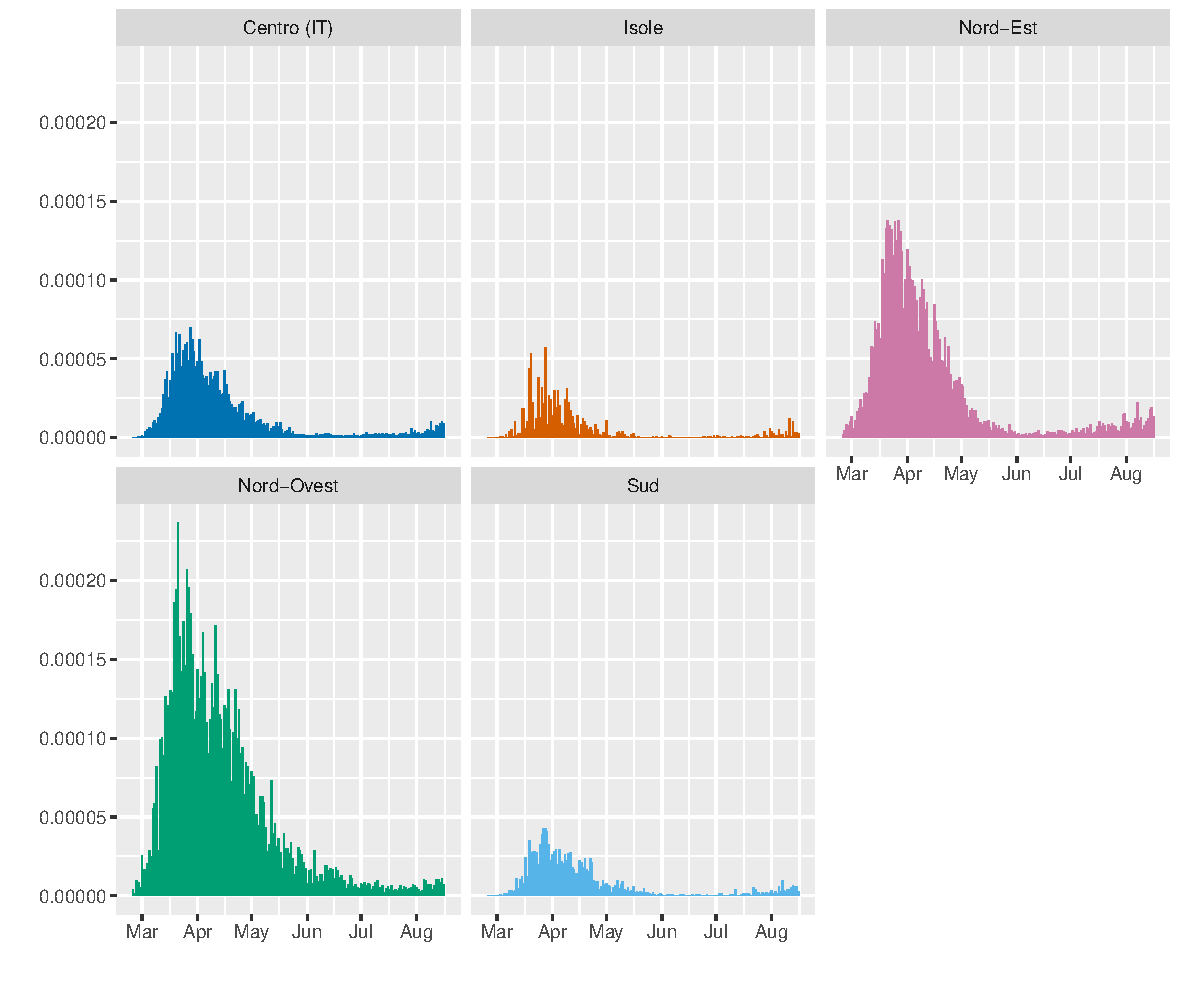
\includegraphics[width=0.92\textwidth]{output/infective_rate_per_NUTS1.pdf}
	    \caption{Incidence rate per NUTS 1 region.}
	    \label{fig:incidence_per_NUTS1}
	\end{figure}
	
	In Figure \ref{fig:incidence_per_NUTS1}, we can see that there is a wide difference in the incidence rates between these larger regions. Not only do we see that the heights of the peaks differ, we also notice that the length of the peaks differ slightly over the regions. This already shows that models that pool these regions together, to form Italy as a whole, are likely less suitable than models that take these differences into account. \\
	
	Consider Figure \ref{fig:incidence_Centro}, where we zoom in on the Centro (IT) NUTS 1 region by looking at the four regions that make it up. These lower level regions are called the NUTS 2 regions. The plots for the other NUTS 1 regions can be found in Appendix \ref{sapp:figures_problem_description}. 
	
	\begin{figure}[H]
	    \centering
	    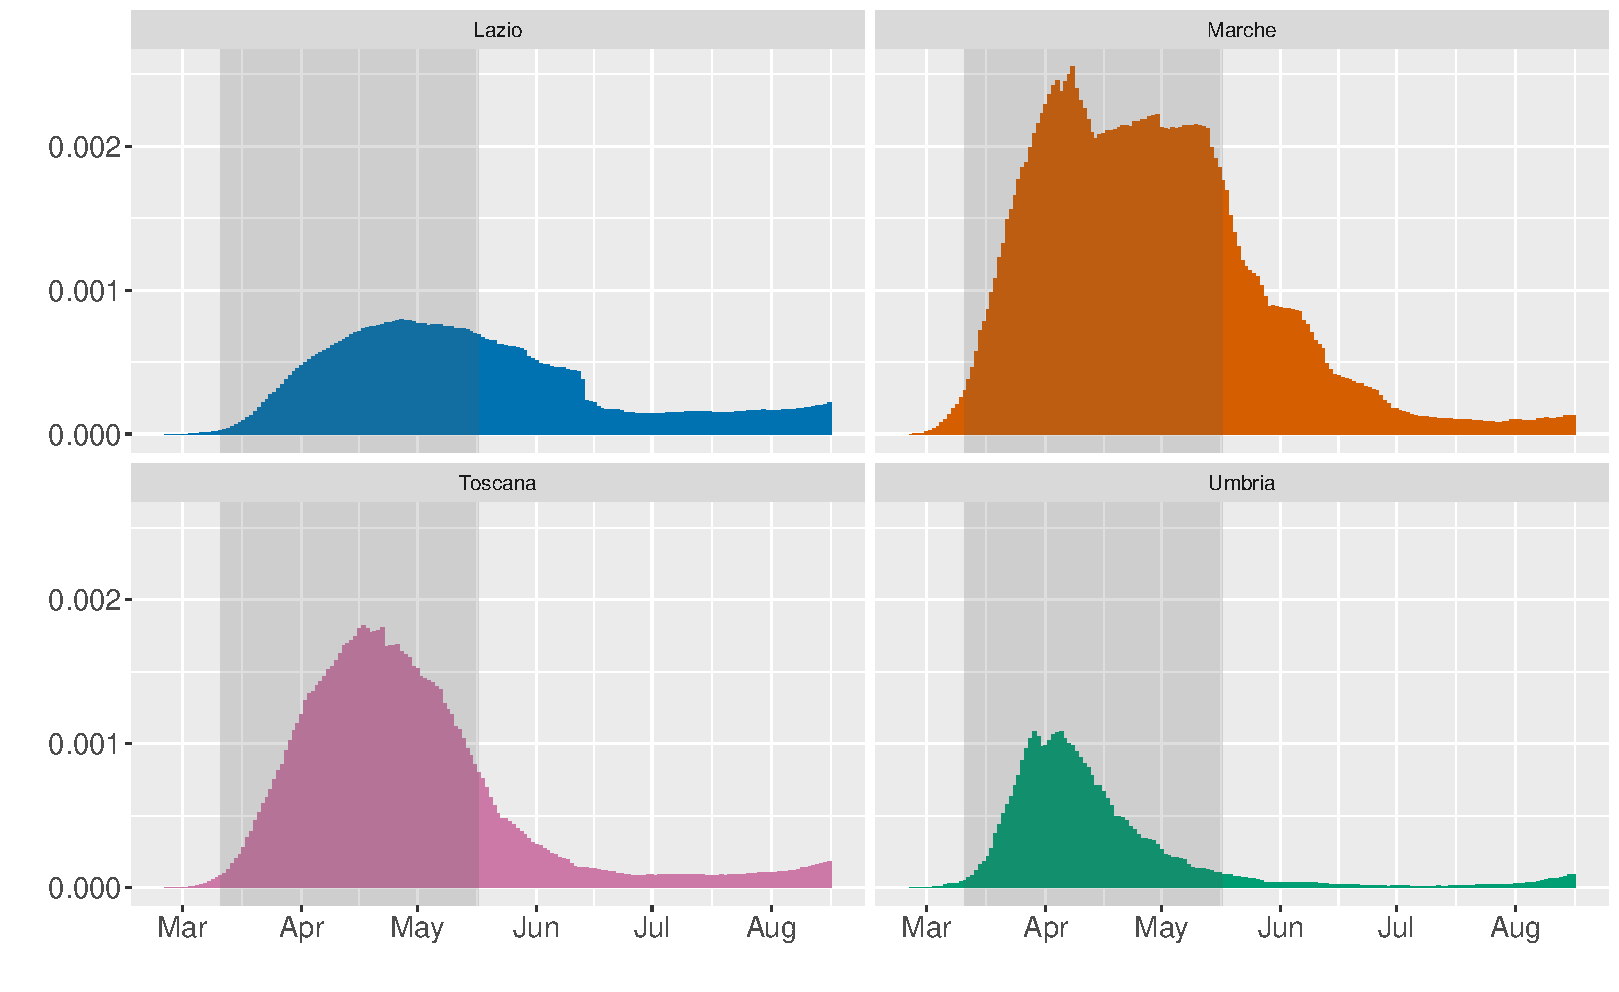
\includegraphics[width=0.92\textwidth]{output/infective_rates_Centro (IT).pdf}
	    \caption{Incidence rate per NUTS 2 region for the Centro (IT) NUTS 1 region.}
	    \label{fig:incidence_Centro}
	\end{figure}
	
	Figure \ref{fig:incidence_Centro} shows that, even among the regions in the NUTS 1 region, there is a vast difference. For the region of Lazio, we see a much lower peak than for the other three regions, especially compared to Marche. Moreover, the varying length of the peak is more visible in Figure \ref{fig:incidence_Centro}, for example when comparing the regions of Marche and Umbria. \\
	
	We also investigate the regional heterogeneity by looking at the mean incidence rate over time across the regions. We consider the mean incidence rate because this allows us to compare regions, even when these have a higher population county. A caveat should be made that there may be heterogeneity in the transmission that may be independent of the mean amount of cases. However, investigating the mean incidence rate may give us some sort of idea of how the pandemic has impacted the regions, at least on average. Consider Figure \ref{fig:heterogeneity_over_regions}, which shows the mean incidence rate for the NUTS 2 regions, divided up into their respective NUTS 1 regions. Along with the mean incidence rate, we present an error bar the size of two times the standard error.
	
	\begin{figure}[H]
	    \centering
	    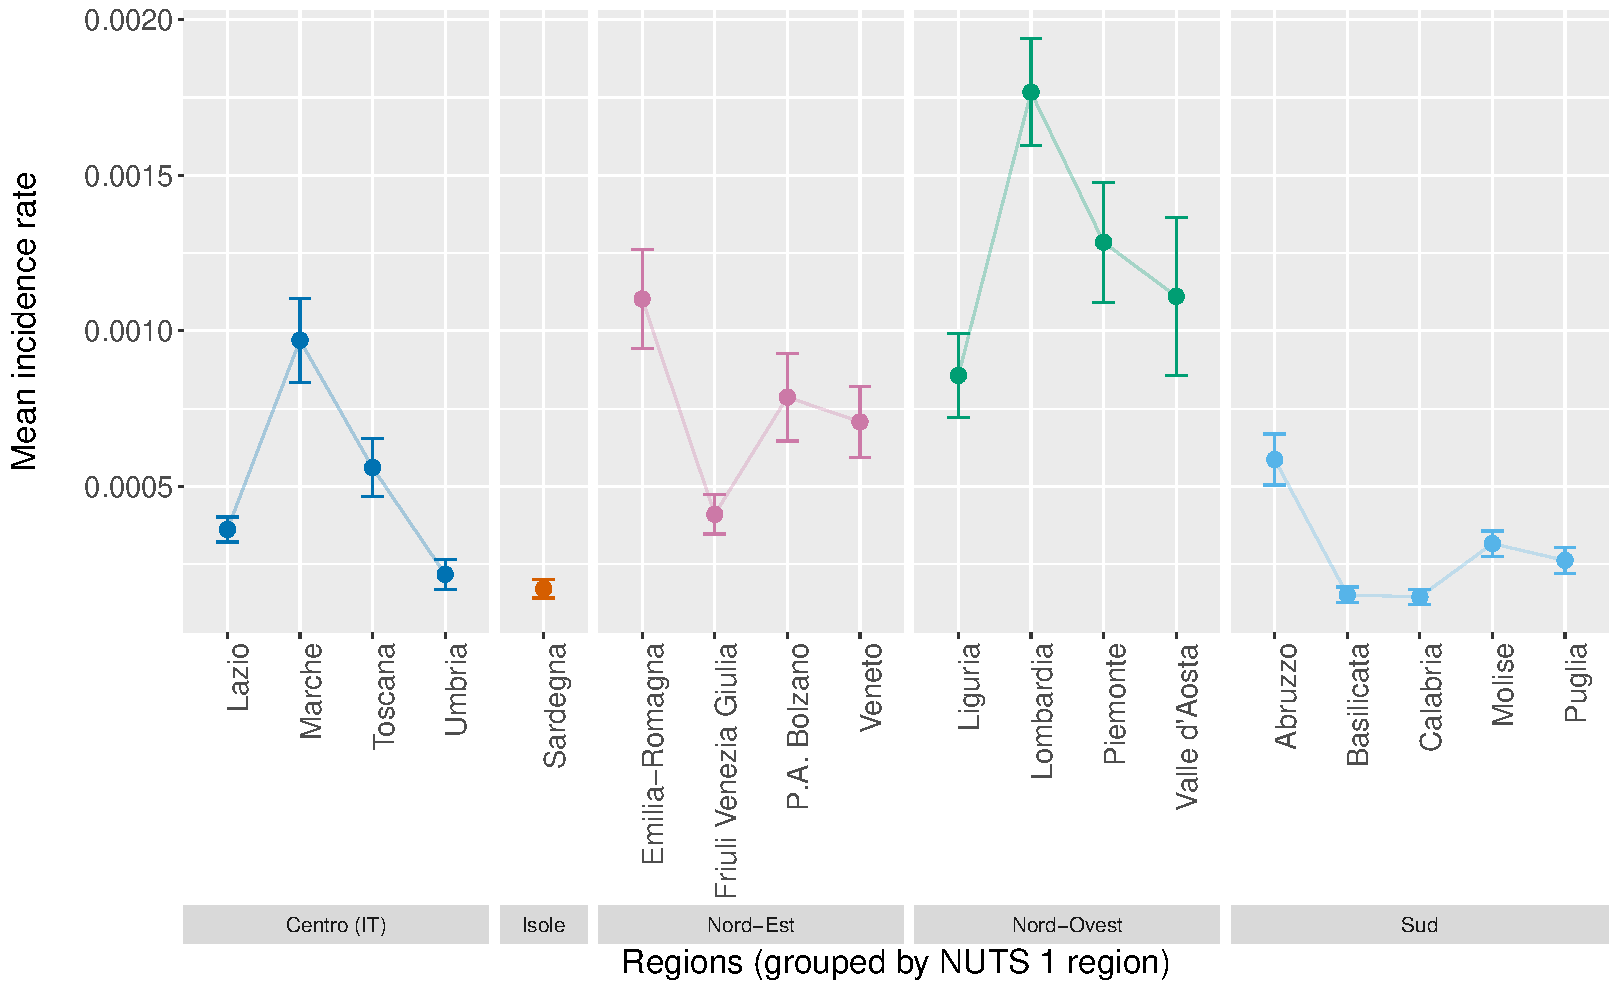
\includegraphics[width=0.92\textwidth]{output/heterogeneity_over_regions.pdf}
	    \caption{Heterogeneity across Italian regions.}
	    \label{fig:heterogeneity_over_regions}
	\end{figure}
	
	From Figure \ref{fig:heterogeneity_over_regions}, we can see that there is a large difference in the mean incidence rate over the different regions. Although we see that the mean incidence rates within the same NUTS 1 region are more similar than outside these regions, there is still a proper difference among regions, even in the same NUTS 1 region. To illustrate, consider the Nord-Est NUTS 1 region. The mean of P.A. Bolzano (Autonomous Province of Bolzano) cannot be statistically distinguished with that of Emilia-Romagna and Veneto, which can be concluded because the given error bars overlap. However, it can be distinguished from the mean incidence rate of Friuli Venezia Giulia, because these error bars do not overlap. This shows us that the heterogeneity between regions may be an issue. \\
	
	In this thesis, we present several models. We are basing the models on specifications presented by \textcite{adda2016economic}. In the paper, \textcite{adda2016economic} investigates the spread of several viral diseases in the past, namely for influenza, gastroenteritis, and chickenpox. The models used to research this spread are inspired by the Standard Inflammatory Response (SIR) model but deviate from the SIR model in the sense that the variables include the number of new cases rather than the absolute number of cases. The key additions made by \textcite{adda2016economic} are, firstly, that a spatial spillover effect is considered and, secondly, that some sort of weighting on the parameters is allowed on the basis of region specific variables. With this motivation, \textcite{adda2016economic} defines three models comprising of a model ignoring interaction between regions, a model taking interaction between regions into account, and a model that expands on the latter by introducing the weights. Unfortunately, good weighting variables regarding SARS-CoV-2 are not available due to the temporal limitations of the data. \textcite{adda2016economic} looks at viruses that have been appearing in society for several years and can, therefore, use weekly information and relevant instruments to quantify the infection rates, such as economic indices. Given that SARS-CoV-2 has only been appearing for around half a year, this information is not available. Consequently, this thesis only discusses the non-weighted models by \textcite{adda2016economic}. These models have not previously been applied to SARS-CoV-2 and can possibly show interesting insights compared to other models.
	
	\section{Dataset} \label{sec:dataset}
	% Dataset and explanations
	In this section, we outline the structure of the data that is used and how it was retrieved. Firstly, we discuss the structure of Italian regions in Section \ref{subsec:italy_geography}. Subsequently, we look at the data on COVID-19 such as the incidence rate, reported deaths, and number of recoveries in Section \ref{subsec:coronavirus_data}. Here, we also discuss how possible errors and missing values in the data are handled. Lastly, Section \ref{subsec:regressor_data} discusses the independent variables that are included in the models by \textcite{adda2016economic}.
	
	\subsection{Geographical Structure of Italy} \label{subsec:italy_geography}
	In this section, we discuss the structure of Italian regions according to the NUTS classification (Nomenclature of Territorial Units for Statistics, from the French \textit{Nomenclature des Unités Territoriales Statistiques}). This is a hierarchical system for dividing up the economic territory of the European Union and the United Kingdom \parencite{background-nuts}. Italy consists of five first-level NUTS regions (also called NUTS 1 regions), namely \textit{Nord-Ovest} (North-West), \textit{Nord-Est} (North-East), \textit{Centro (IT)} (Center), \textit{Sud} (South), and \textit{Isole} (Islands). These larger regions are subdivided into 21 second-level NUTS regions (also called NUTS 2 regions), known as \textit{regioni}. These \textit{regioni} are comparable to Dutch provinces. The \textit{regioni} of \textit{Trentino-Alto Adige} (Trento-South Tyrol) is split into two NUTS 2 regions: \textit{Provincia Autonoma di Bolzano/Bozen} and \textit{Provincia Autonoma di Trento}. The third-level NUTS regions (also called NUTS 3 regions) are 107 administrative subregions of the \textit{regioni}. Figure \ref{fig:map_italy} presents a map of Italy with the NUTS 2 regions.\footnote{Source: \url{https://www.geocurrents.info/cartography/customizable-base-maps-of-italy}}
	
	\begin{figure}[H]
	    \centering
	    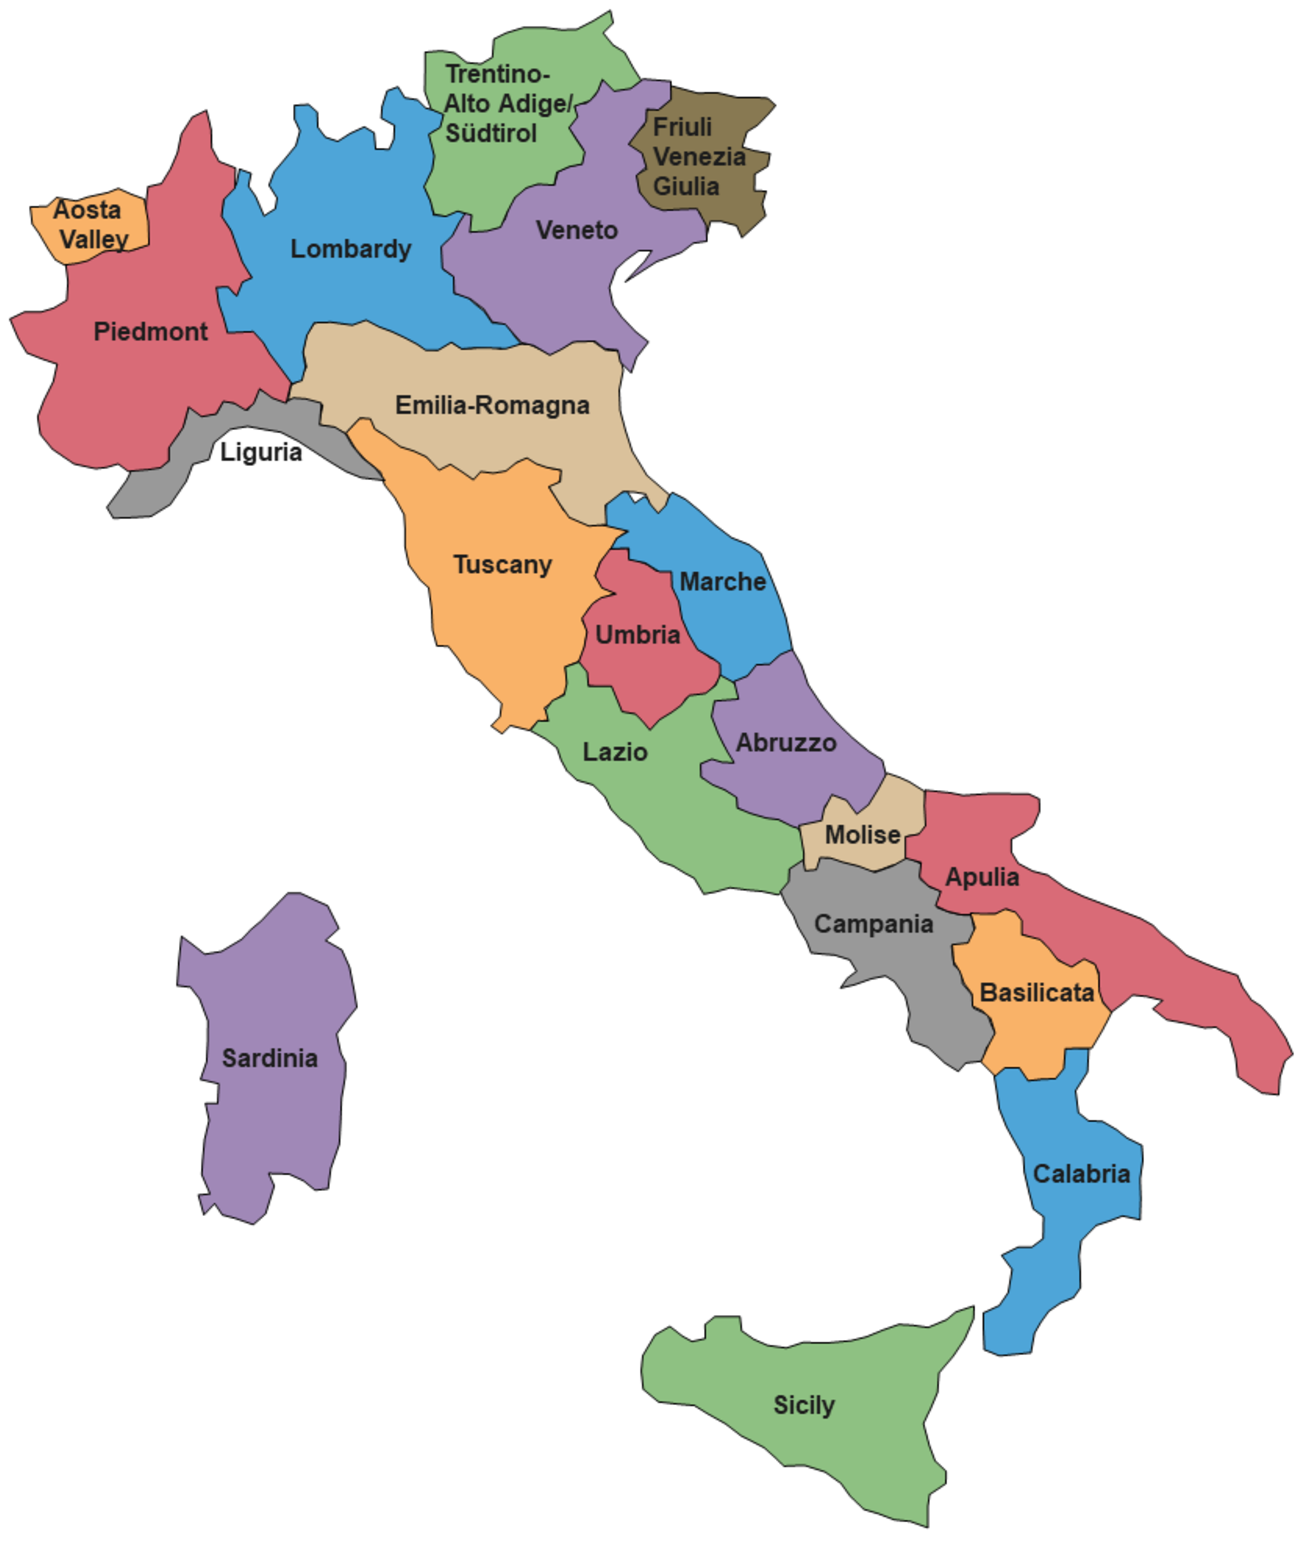
\includegraphics[width=0.8\textwidth]{output/Italy-Map.pdf}
	    \caption{Map of Italy and the NUTS 2 regions that make it up.}
	    \label{fig:map_italy}
	\end{figure}
	
	\subsection{Coronavirus Data} \label{subsec:coronavirus_data}
	In this section, we discuss the data on COVID-19 and how we handled the data processing. The \textit{Presidenza del Consiglio dei Ministri - Dipartimento della Protezione Civile} (Presidency of the Council of Ministers - Department of Civil Protection), hereafter referred to as the Department of Civil Protection, has posted daily reports containing tables with a detailed numerical overview of new cases, active intensive care (IC) patients, tests executed, and more \parencite{Rosini2020Github}. This data is divided up between the NUTS 2 regions. Ideally, we would want to have coronavirus data on the NUTS 3 regions since many policies are introduced at that level, such as a lockdown put into place on March 7, 2020 until the strict national lockdown was instated. Unfortunately, the data outside of the total number of cases was not reported at this granular level. As such, we choose to use the NUTS 2 regions. \\
	
	For $P = 21$ Italian regions, we retrieved the data on COVID-19 from February 25, 2020, until August 16, 2020, leading to observations for $T = 174$ days and a total number of $P \times T = 3,654$ observations. The statistics that are of interest to us are:
	\begin{itemize}
	    \item New number of current positive cases (\textit{nuovi\_positivi});
	    \item Total number of deaths (\textit{deceduti});
	    \item Total number of recoveries (\textit{dimessi\_guariti});
	    \item Total number of positive cases (\textit{totale\_casi});
	    \item Total number of tests performed (\textit{tamponi});
	    \item Total number of people tested (\textit{casi\_testati}).
	\end{itemize}
	
	In addition to these variables, the report also contains, for instance, the number of active ICU cases (\textit{terapia\_intensiva}) and the number of hospitalized people who showed symptoms (\textit{ricoverati\_con\_sintomi}).\footnote{Official data descriptions of all variables can be found at \url{https://github.com/pcm-dpc/COVID-19/blob/master/dati-andamento-covid19-italia.md}} \\
	
	The data source states that the new number of current positive cases at time $t$, namely \textit{nuovi\_positivi}, is calculated as the first difference of the total number of positive cases: $(totale\_casi_t - totale\_casi_{t-1})$. However, in the data these two are not always equal. To illustrate, we consider the region of Abruzzo on June 16 until June 18. The daily number of positive tests $(totale\_casi_t - totale\_casi_{t-1})$ equal 1, 0, and -1, respectively, while the number of new confirmed cases (\textit{nuovi\_positivi}) equal 2, 2, and 1, respectively. This is likely a measurement or computational error. We take the first difference of the total number of positive cases to define the number of confirmed cases rather than looking at the new number of positive cases reported. \\
	
	There are two variables on the tests executed. The semantic difference between the total amount of tests performed (\textit{tamponi}) and the total amount of people tested \textit{(casi testati)} is that the latter indicates the number of unique persons that were tested because individuals could have been tested more than once. Notice that \textit{tamponi} is a good indication of the testing capacity as the number of tests that Italy is able to execute. Henceforth, when the term \textit{testing capacity} is used, this refers to \textit{tamponi}, unless indicated otherwise. In addition to the previous remarks, it is important to consider that there is a measurement error in the number of infectives, as is the case in any other country. This is because there is no possibility that every citizen can be tested for COVID-19. For that reason, the actual number of infectives is higher that the official count as reported in the tables of the Department of Civil Protection. In Section \ref{sec:undocumented_modelling}, we discuss how the undocumented infectives are modelled. \\
	
	With respect to the reported death statistics, there is a distinction between Italy and some other European countries. Namely, the Italian numbers include deaths of all patients who were tested positive for COVID-19 before or after their death. On the other hand, Belgian death counts, for instance, also include deaths of people who were suspected of having COVID-19, regardless of whether they were tested or not \parencite{schultz2020belgiumDeathRate}. Moreover, Italian data makes no distinction between people who died because of COVID-19 and those who simply had the disease but who died from other causes (also referred to as comorbidities). Actually, only 1.2\% of the Italian patients who were reported to have died because of COVID-19 until March 19, 2020 did not have a pre-existing condition \parencite{ecdc2020riskassessment}. Of the patients that died and did have at least one comorbidity, 48.6\% had three or more comorbidities, 26.6\% had two comorbidities, and 23.5\% had one comorbidity. \textcite{ecdc2020riskassessment} also reports that 73.8\% of the deceased patients had hypertension, 33.9\% diabetes, 30.1\% ischaemic heart disease, 22.0\% atrial fibrillation, and 19.5\% had a cancer diagnosed in the last five years. As such, it may be the case that a patient died from, for instance, hypertension but because they were infected by SARS-CoV-2 their death was classified as a COVID-19 death instead. Some other countries, such as Germany, do make a distinction between these two groups  \parencite{otherCountriesDeathsCaccia}. In the UK, there is a radical difference between the total number of deaths until June 28 with a positive test result (43,575 deaths), the total number of deaths until June 19 where COVID-19 is mentioned on the death certificate (53,858 deaths), and the total number of deaths until June 19 over and above the usual number at that time of the year (65,132 deaths) \parencite{bbc2020deathrate}. This shows that the UK reports deaths due to COVID-19 on the death certificates even for people who were not tested positive. Moreover, there are many excess deaths over the usual number that may or may not be due to COVID-19 that are now not counted in the official reports. In this thesis, we assume that this error is negligible and that this differing method of counting deaths and cases only applies on a national level and not among a country's regions. \\
	
	Sometimes, regions correct mistakes by having the numbers in the report on a day compensate for the errors on the days before. In the official publications that we use, data that was wrongly published on a day $t-1$ is corrected by subtracting the error from or adding the error to the cases from day $t$. As such, if the error is larger than the number of new cases, the reported amount of new cases is negative. It happened twenty-two times that the number of confirmed cases was reported to be negative (for eleven different regions). The number of deaths was reported to be negative eight times (for six different regions) and the number of recovered patients was reported with a negative value 62 times (for fourteen different regions). We correct this by subtracting the error from the day before and set the previously negative number to zero. In the case that the error on day $t$ is larger than the number on $t-1$, for instance if a value of $\shortminus10$ is reported on day $t$ while the value for day $t-1$ is less than ten, we propagate the error to multiple lags until this issue no longer occurs. An example for the region of Basilicata is given in Table \ref{tab:example_propagation_negative_values}.
	
	\begin{table}[H]
		\centering
		\caption{Example of the propagation of negative values for the region of Basilicata.}
		\label{tab:example_propagation_negative_values}
		\begin{tabular}{llllll}
			\toprule
			Date    & Original values   & Step 1 & Step 2 & Step 3 & Final step \\ \midrule
            May 3   & 6                 & 6      & 6      & 6      & 2          \\
            May 4   & 0                 & 0      & 0      & 0      & 0          \\
            May 5   & 10                & 10     & 10     & -4     & 0          \\
            May 6   & 3                 & 3      & -14    & 0      & 0          \\
            May 7   & -16               & -17    & 0      & 0      & 0          \\
            May 8   & -1                & 0      & 0      & 0      & 0          \\ \bottomrule
		\end{tabular}
	\end{table}
	
	For days where the correction did not cause the number to become negative, we have no way of detecting that a correction took place and we cannot reasonably assume how this number should be split up among the days concerned. As such, these are left as is. Despite these errors, we assume that the official information is accurate and representative of the region for which it has been reported. \\
	
	A highly negative value of $-229$ was reported for the region of Campania on June 12, 2020, whereas the number of new cases in the week before that date only ranges from zero to five. The same applies to Sicily, where a negative value of $-394$ was reported on June 19, 2020. There, the number of new cases in the week before that date only ranges from zero to two. We assume that this corrects for all errors in the past, not just those close to June 12 and 19. Propagating this error backwards as described before would lead to zero new cases per day for Campania from May 13 until June 12 (31 days) and for Sicily from April 28 until June 19 (53 days). Since we have no reason to know how this error is distributed, we remove the regions of Campania and Sicily from our dataset. Another solution could be to distribute the error according to the daily number of cases relative to the total amount of cases until June 12 for Campania or June 19 for Sicily. \\
	
	An extreme outlier in the positive direction can be found on June 24 for the region of Trentino. A value of 387 new infectives was reported even though in the four weeks before, the maximum amount of new infectives was seven. Notably, this value is the highest of all reported values for Trentino, with the second highest value only being 172 on March 15. For the same reason as mentioned for the high negative values for Campania and Sicily, we remove the region of Trentino from our dataset. Again, another solution would be to distribute this number across the days prior. \\
	
	Regarding missing values, there are none. We expect that this is because the Department of Civil Protection imputed the missing values with a value of zero. For instance, on July 5, it was reported that zero tests were executed in the region of Basilicata. On the dates surrounding July 5, however, around 250 tests were executed each day. On July 9, a higher value of 426 was reported. We expect that this is to correct for the reported value of zero of July 5. We could, for instance, distribute the 426 among July 5 and 9. However, in this thesis, we do not deal with these outliers and leave them as is. The reason for this is twofold. Firstly, we do not know if it is actually true that a zero is being used as a filler for a missing value. It may be the case that a value of zero was actually reported. That relates to the second reason, namely that unexpectedly low values unequal to zero are also reported (such as a value of three tests being executed on July 19 for Basilicata among a usual value of around 300). As such, we cannot reasonably assume that these zeros (and which ones) pertain to missing values.
	
	\subsection{Independent Variables} \label{subsec:regressor_data}
	In this section, we describe the independent variables, or regressors, that are included in the models by \textcite{adda2016economic}. Both models include a tensor $X$ with variables that may not directly have an effect on the transmission rate. We noticed in Section \ref{sec:problem_description} that there is a difference between the case of SARS-CoV-2 and the viruses investigated by \textcite{adda2016economic}, namely due to the time dimension. SARS-CoV-2 has only been appearing in society since December 2019 and, hence, we do not have much time-varying information, for instance on seasonality of the virus as well as economic indicators for the Italian regions. Therefore, we cannot include many variables in our tensor $X$. The only variable that is included is a dummy variable that denotes if the day $t$ is on the weekend (Saturday or Sunday). We do not include an intercept because there is not some (non-zero) mean number of new cases that is persistent throughout time for a certain region. \\
	
	The reason behind including the weekend dummy variable is that we expect that less people may be detected on the weekend due to some general practitioner practices or testing locations being closed on the weekend, meaning that people who are not willing or able to travel far will not get tested. These people will then get tested during the week, meaning that we expect that the number of infectives during weekends will be lower. On the other hand, it is unknown whether the reported number of positive tests on a certain day is the amount of people that got tested on that day or the amount of tests that were processed on that day that turned out to be positive. The difference is that there is a time lag between people being tested and the results of that test being processed and announced. Therefore, there could be a delay of one or multiple days.
	
% 	To investigate this conjecture, we plot the mean incidence rate per NUTS 2 region per day of the week in Figure \ref{fig:incidence_Centro_weekday}. For brevity's sake, we display the plot for the Centro (IT) NUTS 1 region. Plots for the other NUTS 1 regions are included in Appendix \ref{sapp:figures_dataset}, which all show a similar result. \\
	
% 	\begin{figure}[ht]
% 	    \centering
% 	    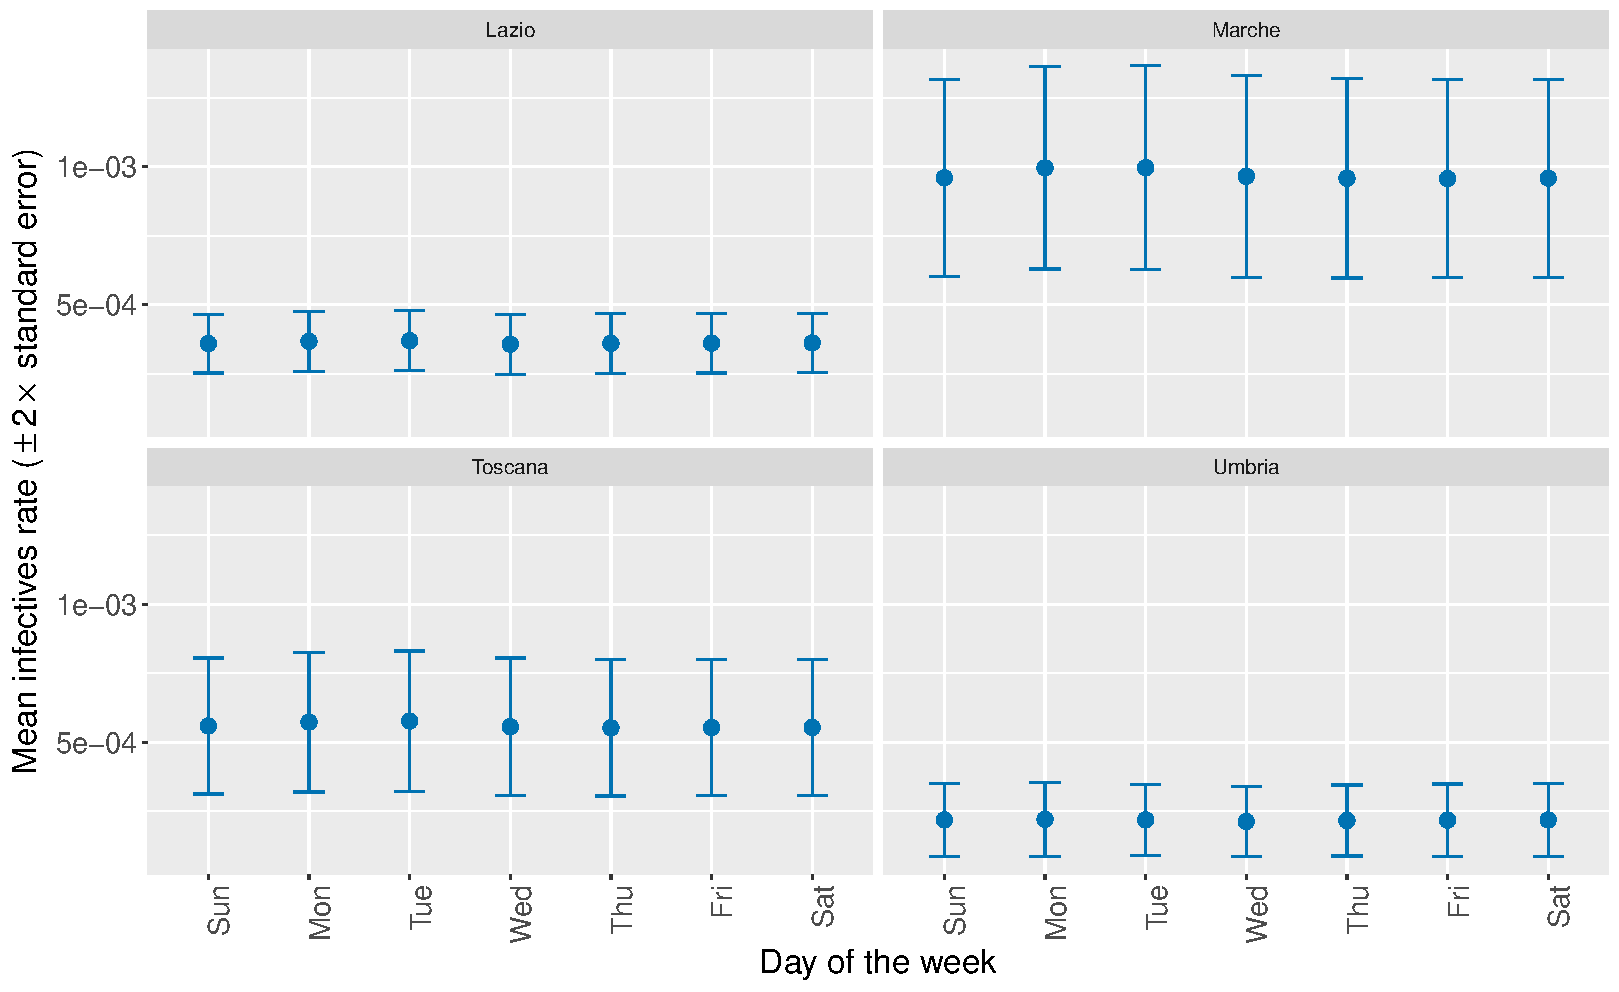
\includegraphics[width=0.98\textwidth]{output/infective_rates_weekday_Centro (IT).pdf}
% 	    \caption{Incidence rate per NUTS 2 region per day of the week for the Centro (IT) NUTS 1 region}
% 	    \label{fig:incidence_Centro_weekday}
% 	\end{figure}
	
% 	\todo[inline, backgroundcolor]{TODO: Update text}
	
% 	Figure \ref{fig:incidence_Centro_weekday} shows us that, although the mean incidence rate for Sunday is usually the highest, there is no statistical evidence to infer that there is a higher incidence rate on certain days. This can be concluded because the given error bars of two times the standard deviation overlap. As such, our intuition is likely not as strong on this subject. Nonetheless, we include the variable in the model because an inspection in isolation is not necessarily an indication that the variable is not predictive for the intended dependent variable.
	
	\section{SIR Model}\label{sec:sir_model}
	In this section, we explain the most commonly used model in epidemiology, namely the Standard Inflammatory Response (SIR) model \parencite{kermack1927contribution, anderson1992infectious}. The SIR model splits the total population into three groups. $S$ denotes the fraction of individuals who are susceptible to being infected, $I$ denotes the fraction of individuals who are currently infected, also called infectives, and $R$ denotes the fraction of individuals who have been removed from the model, be that because they successfully recovered from the disease or because they have deceased. We furthermore define $s$ to be the number of susceptible individuals, $i$ to be the number of infectives, and $r$ to be the number of recovered individuals, so that $S = s/N$, $I = i/N$, and $R = r/N$, where $N$ is the total population size. As such, at any point in time, we have that
	    \[S,I,R \in [0,1] \text{ and } S+I+R=1.\]
	    \[s,i,r \in [0,N] \text{ and } s+i+r=N.\]
	
	The SIR model makes four main assumptions. Understanding these assumptions also tells us how the model is constructed. The first assumption is that the population is constant, meaning that births and deaths are ignored. There exist other models in epidemiology that take both of these into account but these are not considered in this thesis due to a lack of data. The second assumption that is made under the SIR model is that there is a time-constant rate of change in infectives, proportional to the interaction between the infectives and the susceptible population. This is represented by the parameter $\beta$, also called the \textit{transmission rate} or the \textit{force of infection} \parencite{keeling2011modeling}. The third assumption that the SIR model makes is that there is a constant rate of change $\gamma$ at which infectives recover or decease. This is a biological parameter that depends on the type of the virus and the strain, thereby not being influenced much by public health interventions \parencite{adda2016economic}. \\
	
	Finally, we assume that there is a constant rate of change $\omega$ at which immune individuals lose their immunity. For instance, \textcite{adda2016economic} mentions that $\omega$ is set to 0 for chickenpox as individuals acquire a lifetime immunity while $\omega$ will be high for gastroenteritis due to almost no immunity emerging. In the case of COVID-19, some studies show that it is likely that individuals who recovered from COVID-19 may be immune to reinfection, at least temporarily \parencite{kirkcaldy2020covid}. This can be challenged because it is currently still unknown whether immunity is always achieved, especially among those who have had only light to medium symptoms. \textcite{leung_2020} estimates that COVID-19 antibodies will remain in a patient’s system for two to three years, based on what is known about other coronaviruses, indicating a possibility of temporary immunity. However, it has recently become clear that reinfection is indeed possible. Two Chinese persons have been tested positive in August after having recovered from COVID-19 a few months prior \parencite{bloomberg2020reinfection}. Future research could be done to incorporate this new information. In this thesis, for simplicity's sake, we assume that lifelong immunity is achieved, or at least long enough to last through the temporal scope of our analysis: we set $\omega = 0$. \\
	
	Now that the assumptions are clear, we present the definition of the SIR model. The SIR model is postulated in continuous time, i.e. the equations in \eqref{eq:SIR_model_S}, \eqref{eq:SIR_model_I}, and \eqref{eq:SIR_model_R} depict the change in the variables $S$, $I$, and $R$, respectively, for one time period ahead.
	
	\begin{align}
    	\frac{dS}{dt} &= -\beta SI + \omega R, \label{eq:SIR_model_S}\\
    	\frac{dI}{dt} &= \beta SI - \gamma I, \label{eq:SIR_model_I}\\
    	\frac{dR}{dt} &= \gamma I - \omega R. \label{eq:SIR_model_R}
	\end{align}
	
	This type of model is also called a stock-and-flow model because there is a certain stock at some point in time (for instance the number of infectives) to which a flow is added and/or subtracted. \textcite{keeling2011modeling} state that the SIR model can also be described by density-dependent transmission instead of frequency-dependent transmission. By that, they mean that the variables $s$, $i$, and $r$ are used instead of $S$, $I$, and $R$. This is given by:
	
	\begin{align}
    	\frac{ds}{dt} &= -\beta si + \omega r, \label{eq:SIR_model_X}\\
    	\frac{di}{dt} &= \beta si - \gamma i, \label{eq:SIR_model_Y}\\
    	\frac{dr}{dt} &= \gamma i - \omega r. \label{eq:SIR_model_Z}
	\end{align}
	
	One of the main measures resulting from the SIR model is the estimation of the effective reproduction number $R_{eff} \coloneqq \beta / \gamma$. An epidemic is said to develop if $R_{eff} > 1$. This is clear because $R_{eff} > 1$ implies that $\beta > \gamma$, i.e. the spread of the virus exceeds the recovery rate: individuals in a society become infected more quickly than they recover. The reproduction number $R_{eff}$ is widely used to indicate whether an ongoing epidemic is dying out. For instance, the Italian health ministry has posted an article on May 9, 2020 to communicate that the $R_0$, being the basic reproduction rate, for COVID-19 was below 1 in Italy, at between 0.5 and 0.7 \parencite{saluteR0}.
	
	\section{Model Selection} \label{sec:model_selection}
	In this section, we explain how model selection is carried out. One can imagine that the same model specification does not apply to all Italian regions. For this reason, we apply model selection. We use the Akaike Information Criterion or AIC \parencite{akaike1974new}. The AIC for a particular model is defined as
	\begin{equation} \label{eq:AIC}
    	AIC = -2\log(ML) + 2k,    
	\end{equation}
	where $ML$ denotes the maximum likelihood for the model and $k$ denotes the number of parameters in the model. In contrast, one could also consider the Bayesian Information Criterion or BIC \parencite{schwarz1978estimating}. \textcite{schwarz1978estimating} developed it as an alternative to the Akaike Information Criterion. The BIC is defined as
	\begin{equation} \label{eq:BIC}
    	BIC = -2\log(ML) + k\log(n),
	\end{equation}
	where $n$ denotes the sample size. Both the AIC and BIC are used as the minimizer in the model selection; the model that is picked by the model selection procedure is the one with the lowest AIC or BIC. \\
	
	When choosing between the two methods, one should realize that they have different properties, particularly related to consistency. The AIC tends to select a larger model than the BIC. Moreover, if the true model is included in the set of candidate models, and under some additional assumptions, the BIC will select the true model with probability one as $n$ goes to infinity whereas the AIC is not consistent. On the other hand, if the true model is not in the set of candidate models, clearly no method can possibly select the true model. However, the AIC is efficient in the sense that it will asymptotically select the model that minimizes the mean prediction error while the BIC is not efficient \parencite{vrieze2012model}. Proponents of using the AIC over the BIC argue that this shows that the AIC is to be preferred because it is virtually impossible for the true model to be constructed because \textit{``all models are wrong"} \parencite{box1976science}. That does not mean that reality cannot be modelled; some models can be useful despite not being perfectly true. \textcite{burnham2002practical} state that \textit{``A model is a simplification or approximation of reality and hence will not reflect all of reality. [...] While a model can never be ``truth," a model might be ranked from very useful, to useful, to somewhat useful to, finally, essentially useless".} Lastly, \textcite{vrieze2012model} shows by simulation that the BIC can fail in finite sample sizes even if the true model is in the candidate set. This is because the BIC has a higher maximum risk, defined as the mean squared error of estimating the true covariance matrix. Because we believe that, indeed, the true model generating the data will quite likely not be included in our candidate set, we use the AIC to perform model selection rather than the BIC.
	
	\section{Modelling Undocumented Infectives} \label{sec:undocumented_modelling}
	In this section, we discuss how our method for modelling undocumented infectives is constructed. We talk about the assumptions, the formulation, and the empirical impact that this has on the total number of infectives. A common concern with the spread of viruses, especially one spreading as rapidly as SARS-CoV-2, is that there is no possibility to test the entire population for the disease because the testing capacity is simply not there. If this were possible, then all individuals who were tested positive could be isolated and the spread of the virus would be dampened tremendously. However, since this is not possible, there are likely many infectives in society who spread the virus but who are undocumented. In China, around 86\% of the infectives went undocumented. These undocumented infectives were estimated to also be contagious, at a level of around 55\% of the contagiousness of documented infectives \parencite{li2020undocumented}. \\
	
	\textcite{li2020undocumented} carried out their research during the period from January 10 until January 23, 2020, meaning that there was a lack of major restrictions such as travel bans. The same conditions do not apply to Italy during our research period, as it was under a strict national lockdown. This lockdown was imposed on March 10, 2020. The restrictions were relaxed around May 18, when businesses were allowed to reopen and citizens were allowed free movement within the region they live in, although they were still barred from travelling to other regions unless they had an essential motive \parencite{severgnini2020relaxLockdown}. \textcite{li2020undocumented} make the important note that their results are indeed highly dependent on the specific situation in the country of interest, for instance due to differences in testing, case definition, and reporting. Nonetheless, this research shows that undocumented infectives should be taken into account. Consequently, this thesis aims to model the undocumented infectives. However, we do not account for the lockdown and similar limiting restrictions in our model. Future research could be done to include these restrictions more robustly. \\
	
	Note that, by definition, there is no data on the number of undocumented infectives because, otherwise, these cases would indeed be documented. As such, some assumptions need to be made since we cannot apply \textit{supervised learning} methods (being models where there is data on a dependent variable to predict) to determine the number of undocumented infectives. Mainly, we assume that the number of undocumented individuals is decreasing as the testing capacity increases. Similarly, the number of documented individuals increases in the testing capacity. The logic behind this is clear: as more people are tested, more infectives move from being undocumented to being documented. \\
	
	At a point in time $t$, we denote the testing capacity by $TC_t$. In Section \ref{subsec:coronavirus_data}, we explained how a measure of the testing capacity is obtained. The total number of infected people at time $t$ is denoted by $s_t$. This group can be subdivided into the documented infectives $D_t$ and the undocumented infectives $U_t$ such that $D_t + U_t = s_t$. Therefore, we can denote the documented and undocumented infectives as proportions of the total number of infected people, at any point in time. As mentioned earlier in this section, this proportion may change over time as the testing capacity increases. This proportion is therefore defined as a function of the testing capacity over time:
    	\begin{equation} \label{eq:f_t}
    	f_t \coloneqq f(TC_t),
    	\end{equation}
	such that
    	\begin{equation*}
        	\begin{cases}
            	D_t &= f_ti_t, \\
            	U_t &= (1-f_t)i_t.
        	\end{cases}
    	\end{equation*}
	Notice that the undocumented infectives can then be written as $U_t = \frac{1-f_t}{f_t}D_t$. \\
	
	There are some properties and assumptions that \eqref{eq:f_t} should satisfy. These are as follows:
	\begin{enumerate}[label=(A\arabic*)]
		\item\label{ass:undoc_proportion} Since $f_t$ is a proportion, we need to have that $f_t \in [0,1]$.
		\item\label{ass:undoc_f0} If no one is tested, we assume that there is a certain minimum proportion of infectives who are documented, denoted by $f^{min} \in [0,1]$. That means that $f(0) = f^{min}$. It should be noted that, at any point in time, it should hold that
    	    \begin{align*}
        	    & D_t + U_t < N_t \\
        	    \iff & D_t + \frac{1-f_t}{f_t}D_t < N_t \\
        	    \iff & \frac{1}{f_t}D_t < N_t \\
        	    \iff & f_t > \frac{D_t}{N_t},
    	    \end{align*}
		so $f^{min}$ should be chosen to be larger than $\min\limits_{t}\left\{\frac{D_t}{N_t}\right\}$. If $f_t$ would be lower than the fraction of the population that is documented to be infective, then the total number of infectives in a population would exceed the total number of people living in that population, which is not possible.
		
		\item\label{ass:undoc_fN} Denote the total population at time $t$ as $N_t$. Then, if there is enough testing capacity such that the entire population can be tested, we assume that all infectives will be documented, so that:
		    \[f(N_t) = 1.\]
		This also assumes that the tests that are executed are perfect at determining whether someone actually is infected. However, it is common knowledge that such tests have a certain rate of false positives and negatives. In the case of COVID-19 specifically, positive screening tests are not followed-up (as is usually common practice to confirm a diagnosis) because of scarcity in testing resources and/or prioritization of allocating tests to the sickest patients \parencite{frasier2020tests}. Moreover, \textcite{bmj2020testaccuracy} reports that serological tests for COVID-19 carry with them risks of bias and heterogeneity in their accuracy. Therefore, they state that these serological tests should only be used cautiously for clinical decision making and epidemiological surveillance. For this reason, one could choose to relax the assumption and assume $f(N_t) = f^{max}$ for some $f^{max} \in [0,1]$ set to be a more reasonably perceived value.
		
		\item\label{ass:undoc_monotonicity} As mentioned earlier in this section, $f_t$ needs to be monotonically increasing in $TC_t$, i.e. the proportion of infectives that is documented is increasing in the testing capacity. Mathematically, this means that
		    \[f'(N_t) \geq 0.\]
	\end{enumerate}
	
	We test several forms of the function $f_t$. Derivations are given in Appendix \ref{sapp:derivation_undocumented_infectives}.
	\begin{itemize}
		\item \textbf{Linear form}
		    \begin{equation} \label{eq:linear_functional_form}
		        f_t = \frac{1-f^{min}}{N_t}TC_t + f^{min}.
		    \end{equation}
    		
    	\item \textbf{Quadratic form}\\
    	We specify three functional forms for a quadratic form. First of all, a general form. After this, we discuss two special cases.
    	    \begin{itemize}
    	        \item For the general quadratic form, we assume without loss of generality that $f\left(\frac{1}{2}N_t\right) = \gamma$ for some $\gamma \in \left[\frac{1}{4} + \frac{3}{4}f^{min}, \frac{3}{4} + \frac{1}{4} f^{min}\right]$. Then the formula becomes:
    	            \begin{equation} \label{eq:quadratic_functional_form}
    	                f_t = \frac{2 - 4\gamma + 2f^{min}}{N_t^2}TC_t^2 + \frac{4\gamma - 1 - 3f^{min}}{N_t}TC_t + f^{min}.
    	            \end{equation}
		        If $\gamma \in \left[\frac{1}{4} + \frac{3}{4}f^{min}, \frac{1}{2} + \frac{1}{2}f^{min}\right)$, the function is upwards opening. If $\gamma \in \left(\frac{1}{2} + \frac{1}{2}f^{min}, \frac{3}{4} + \frac{1}{4} f^{min}\right]$, the function is downwards opening. If $\gamma = \frac{1}{2} + \frac{1}{2}f^{min}$, then the formula simplifies to the linear specification. In Appendix \ref{ssapp:quadratic_derivation}, we explain why $\gamma$ cannot be below $\frac{1}{4} + \frac{3}{4}f^{min}$ or above $\frac{3}{4} + \frac{1}{4} f^{min}$.
		        
		        \item The first special case is the downwards opening vertex form. We assume that the vertex (the extremum) is the point $(N_t, 1)$, i.e. the parabola is downwards opening. Recall that any quadratic function can be rewritten to the so-called vertex form $f(x) = a(x - h)^2 + k$, where the vertex of the function is $(h, k)$. Choosing this special case means that there will be no unknown parameters needed to define the function because we know the location of the vertex and a known point $(0, f^{min})$ on the parabola. We can then derive that the formula becomes:
		            \begin{equation} \label{eq:quadratic_downwards_functional_form}
		                f_t = \frac{f^{min}-1}{N_t^2}TC_t^2 - \frac{2(f^{min}-1)}{N_t}TC_t + f^{min}.
		            \end{equation}
		        
		        This is equivalent to \eqref{eq:quadratic_functional_form} for $\gamma = \frac{3}{4} + \frac{1}{4} f^{min}$. Therefore, this is a boundary case for a downwards opening quadratic function.
		        
		        \item The second special case is the upwards opening vertex form. For the same reason as for the previous specification, we assume that the vertex is the point $(0, f^{min})$, i.e. the parabola is upwards opening. We can then derive that the formula becomes:
		            \begin{equation} \label{eq:quadratic_upwards_functional_form}
		                f_t = \frac{1-f^{min}}{N_t^2}TC_t^2 + f^{min}.
		            \end{equation}
		            
		        This is equivalent to \eqref{eq:quadratic_functional_form} for $\gamma = \frac{1}{4} + \frac{3}{4}f^{min}$. Therefore, this is a boundary case for an upwards opening quadratic function.
		    \end{itemize}
		    
		\item \textbf{Cubic form}\\
		For the cubic form, we assume without loss of generality that $f\left(\frac{1}{4}N_t\right) = \gamma_1$ and $f\left(\frac{1}{2}N_t\right) = \gamma_2$ for some $\gamma_1, \gamma_2 \in (0,1)$ such that $\gamma_1 < \gamma_2$. Then the formula becomes:
		    \begin{equation} \label{eq:cubic_functional_form}
		        \begin{split}
            		f(TC_t) = &\frac{8 + 64\gamma_1 - 48\gamma_2 -24f^{min}}{3N_t^3}TC_t^3 \\
            		&+ \frac{-2 - 32\gamma_1 + 20\gamma_2 + 14f^{min}}{N_t^2}TC_t^2 \\
            		&+ \frac{1 + 32\gamma_1 - 12\gamma_2 - 21f^{min}}{3N_t}TC_t + f^{min}.
        		\end{split}
		    \end{equation}
		    
	    No bounds on $\gamma_1$ and $\gamma_2$ have been set. Particularly, there are combinations of $\gamma_1$ and $\gamma_2$ for which the codomain of $f_t$ on $TC_t \in [0,N_t]$ may not be the interval $[0,1]$, violating assumption \ref{ass:undoc_proportion}, and for which the function is not monotonically increasing, violating assumption \ref{ass:undoc_monotonicity}. One could derive explicit conditions on possible combinations for $\gamma_1$ and $\gamma_2$ such that this is not the case but this is not done in this thesis.
	\end{itemize}
	
	These definitions can easily be generalized to be applicable to regions by considering the total population in a region $N_{p,t}$ instead of the total population $N_t$. Then, the function would be dependent on $p$ as well: 
	\begin{equation} \label{eq:f_rt}
	f_{p,t} \coloneqq f(TC_{p,t}).
	\end{equation}
	such that
	\begin{equation*}
	    \begin{cases}
	        D_{p,t} &= f_{p,t}i_{p,t}, \\
	        U_{p,t} &= (1-f_{p,t})i_{p,t}.
	    \end{cases}
	\end{equation*}
	
	% Make plots
	In Figure \ref{fig:functional_forms}, we specify several functional forms for the specifications as mentioned above. Figure \ref{fig:functional_forms_quadratic} shows four different functional forms for the quadratic functional forms while Figure \ref{fig:functional_forms_cubic} shows four different functional forms for the cubic specification.
	
	% Quadratic
	\def\N{100}
	\def\fmin{0.1}
	
	\begin{figure}[ht]
    \centering
    \resizebox{\columnwidth}{!}{
    \begin{subfigure}[pt]{0.5\linewidth}
    \begin{tikzpicture}
        \begin{axis}[
        xmin = 0, xmax = \N,
        ymin = 0, ymax = 1,
        xlabel=Testing capacity $\left(\frac{TC_{p,t}}{N_{p,t}}\times 100\%\right)$,
        ylabel=Proportion of documented infectives ($f_{p,t}$),
        grid = both,
        minor tick num = 1,
        major grid style = {lightgray},
        minor grid style = {lightgray!25},
        legend style={at={(0.5,-0.3)},anchor=north},
        legend cell align=left
        ]
        \addlegendimage{empty legend}
        \addlegendentry{\hspace{-.6cm}\textbf{From top to bottom:}}
        
        \def\gammaquadraticlow{0.4}
        \addplot[domain = 0:\N, samples = 2*\N, smooth, thick, OliveGreen]{
            (2-4*\gammaquadraticlow + 2*\fmin)/(\N^2)*x^2 +
            (4*\gammaquadraticlow - 1 - 3*\fmin)/(\N)*x +
            \fmin};
        \addlegendentry{Quadratic $(\gamma = \gammaquadraticlow)$}
        
        \addplot[domain = 0:\N, samples = 2*\N, smooth, thick, MidnightBlue]{
            (\fmin-1)/(\N^2)*x^2 -
            2*(\fmin-1)/(\N)*x +
            \fmin};
        \addlegendentry{Downwards opening - vertex: $(N_{p,t},1)$}
        
    	\def\gammaquadratichigh{0.7}
        \addplot[domain = 0:\N, samples = 2*\N, smooth, thick, WildStrawberry]{
            (2-4*\gammaquadratichigh + 2*\fmin)/(\N^2)*x^2 +
            (4*\gammaquadratichigh - 1 - 3*\fmin)/(\N)*x +
            \fmin};
        \addlegendentry{Quadratic $(\gamma = \gammaquadratichigh)$}
        
        \addplot[domain = 0:\N, samples = 2*\N, smooth, thick, Black]{
            (1-\fmin)/\N*x + \fmin};
        \addlegendentry{Linear}
        
        \addplot[domain = 0:\N, samples = 2*\N, smooth, thick, RawSienna]{
            (1-\fmin)/(\N^2)*x^2 +
            \fmin};
        \addlegendentry{Upwards opening - vertex: $(0,\fmin)$}
        
        \end{axis}
        \end{tikzpicture}
	    \caption{Quadratic specifications}
	    \label{fig:functional_forms_quadratic}
    \end{subfigure}
    \hspace{8mm}
    
    % Cubic
    \begin{subfigure}[pt]{0.48\linewidth}
        
        \begin{tikzpicture}
        \begin{axis}[
        xmin = 0, xmax = \N,
        ymin = 0, ymax = 1,
        xlabel = Testing capacity $\left(\frac{TC_{p,t}}{N_{p,t}}\times 100\%\right)$,
        ylabel = \textcolor{white}{Proportion of documented infectives ($f_{p,t}$)},
        grid = both,
        minor tick num = 1,
        major grid style = {lightgray},
        minor grid style = {lightgray!25},
        legend style = {at={(0.5,-0.3)}, anchor=north},
        legend cell align = left
        ]
        \addlegendimage{empty legend}
        \addlegendentry{\hspace{-.6cm}\textbf{From top to bottom (at 20\% capacity):}}
        
        \def\gammaoneone{0.65}
        \def\gammatwoone{0.7}
        \addplot[domain = 0:\N, samples = 2*\N, smooth, thick, OliveGreen]{
            (8 + 64*\gammaoneone - 48*\gammatwoone -24*\fmin)/(3*\N^3)*x^3 +
            (-2 - 32*\gammaoneone + 20*\gammatwoone +14*\fmin)/(\N^2)*x^2 +
            (1 + 32*\gammaoneone - 12*\gammatwoone -21*\fmin)/(3*\N)*x +
            \fmin};
        \addlegendentry{Cubic $(\gamma_1 = \gammaoneone, \gamma_2 = \gammatwoone)$}
        
        \def\gammaonetwo{0.6}
        \def\gammatwotwo{0.8}
        \addplot[domain = 0:\N, samples = 2*\N, smooth, thick, WildStrawberry]{
            (8 + 64*\gammaonetwo - 48*\gammatwotwo -24*\fmin)/(3*\N^3)*x^3 +
            (-2 - 32*\gammaonetwo + 20*\gammatwotwo +14*\fmin)/(\N^2)*x^2 +
            (1 + 32*\gammaonetwo - 12*\gammatwotwo -21*\fmin)/(3*\N)*x +
            \fmin};
        \addlegendentry{Cubic $(\gamma_1 = \gammaonetwo, \gamma_2 = \gammatwotwo)$}
        
        \def\gammaonethree{0.5}
        \def\gammatwothree{0.6}
        \addplot[domain = 0:\N, samples = 2*\N, smooth, thick, MidnightBlue]{
            (8 + 64*\gammaonethree - 48*\gammatwothree -24*\fmin)/(3*\N^3)*x^3 +
            (-2 - 32*\gammaonethree + 20*\gammatwothree +14*\fmin)/(\N^2)*x^2 +
            (1 + 32*\gammaonethree - 12*\gammatwothree -21*\fmin)/(3*\N)*x +
            \fmin};
        \addlegendentry{Cubic $(\gamma_1 = \gammaonethree, \gamma_2 = \gammatwothree)$}
        
        \def\gammaonefour{0.35}
        \def\gammatwofour{0.7}
        \addplot[domain = 0:\N, samples = 2*\N, smooth, thick, RawSienna]{
            (8 + 64*\gammaonefour - 48*\gammatwofour -24*\fmin)/(3*\N^3)*x^3 +
            (-2 - 32*\gammaonefour + 20*\gammatwofour +14*\fmin)/(\N^2)*x^2 +
            (1 + 32*\gammaonefour - 12*\gammatwofour -21*\fmin)/(3*\N)*x +
            \fmin};
        \addlegendentry{Cubic $(\gamma_1 = \gammaonefour, \gamma_2 = \gammatwofour)$}
        
        \addplot[domain = 0:\N, samples = 2*\N, smooth, thick, Black]{
            (1-\fmin)/\N*x + \fmin};
        \addlegendentry{Linear}
        
        \end{axis}
        \end{tikzpicture}
	    \caption{Cubic specifications}
	    \label{fig:functional_forms_cubic}
	\end{subfigure}
    }
    
    \caption{Functional forms for the proportion of documented infectives \\($f^{min} = 0.1$)}
    \label{fig:functional_forms}
    \end{figure}
    
    Not all of the plots in Figure \ref{fig:functional_forms} are meant to be realistic portrayals. They simply show how the functions behave as the parameters change. Moreover, recall that there are combinations of $\gamma_1$ and $\gamma_2$ for the cubic representation for which assumptions \ref{ass:undoc_proportion} and \ref{ass:undoc_monotonicity} are violated. Figure \ref{fig:functional_forms_cubic} shows that $\gamma_1=0.35$ and $\gamma_2=0.7$ cause the function to exceed the maximum value allowed for $f_{p,t}$ of 1, violating \ref{ass:undoc_proportion}. A combination of $\gamma_1=0.65$ and $\gamma_2=0.7$ creates a non-monotonic functional form, which violates \ref{ass:undoc_monotonicity}. \\
    
    Next, we argue which of these forms is most appropriate. As mentioned at the beginning of this section, we cannot estimate which form would fit the data best because there is, by definition, no data on the undocumented infectives. As such, we argue which functional form to use by a theoretical rather than an empirical approach. Before that, note that the shape of the functional form may differ depending on the effective reproduction number $R_{eff}$, as defined in Section \ref{sec:problem_description}. $R_{eff}$ estimates how many people an infective will on average infect. If $R_{eff} > 1$, a person is estimated to infect more than one person and an epidemic is expected to develop. In this case, we expect that an increased testing capacity will have a larger immediate effect. We assume that a person who has been tested positive adheres to the common guidelines that they should self-quarantine. Consequently, this infective does not infect other people who would otherwise become undocumented infectives. For the remainder of this argument, we assume that $R_{eff} > 1$. The reason for this is that the results from this thesis will be most important during an epidemic. Future research could be conducted into a two-step approach, where $R_{eff}$ is estimated first so that the method of modelling undocumented infectives can be adapted accordingly. \\
    
    % The main question that we need to ask ourselves is whether the impact of a change in testing capacity is different relative to the initial testing capacity. If the testing capacity is low and we increase it, does that have a different effect on the proportion of documented infectives than when testing capacity is high and we increase it by the same amount? Presumably, it is larger. \\
    
    We first argue why a downwards opening quadratic function fits the requirements well. Note that when a large proportion of the population has been tested, the pool of untested people, who are potentially infectious, is smaller. The probability that they, in isolation of other effects, are infected is lower. The argument for this is as follows: assuming that the people close to them who were tested positive (be that family, acquaintances, or those that they would perhaps run into at the supermarket) do indeed self-isolate, they would not have been able to been in contact with them and they have a lower chance to be infected. When a small number of people is tested and suddenly the testing capacity is increased, a larger pool of people who had symptoms and could previously not be tested, now have access to a test. The people who are now most likely to get tested positive have strong symptoms. As they are now tested positive, we assume they self-quarantine and cannot infect other people. Therefore, the functional form that fits this argument best is a downwards opening quadratic function. \\
    
    One could also consider the cubic representation with $\gamma_1=0.6$ and $\gamma_2=0.8$, or some similar parameter values, as in Figure \ref{fig:functional_forms_cubic}. There, we see similar behaviour at the start of the graph where there is a sharp increase, after which it levels out. The difference is found when there is the testing capacity to test the last proportion of the population, leading to a sudden sharp increase in the proportion of documented infectives. An argument in favour of this specification is that it may be difficult to track down and convince the last proportion of the population to take a test who, at that point, may be infectious. For instance, these may simply be people who do not believe that they should get tested, whether their reasons are grounded or not. Perhaps these people underestimate their symptoms or their importance. They may, even though they are encouraged to get tested, believe that they do not need to be. For instance, these people may feel that others need to get the test more. If these infective people do not get tested, the proportion of documented infectives may level out more quickly. Moreover, these people will only turn up to the testing location if they are convinced that the testing capacity is high enough, leading to a final increase as the capacity approaches 100\%. \\
    
    Weighing these two specifications off, we believe that the argument in favour of a quadratic form is more general and stable, whereas the argument in favour of a cubic form is more specific. In general, of all possible fitting solutions, the one with the least number of assumptions needed is often to be preferred. Therefore, we opt to use a downwards opening quadratic functional form over a cubic form. Now that we have chosen our functional form, the question is what to choose for the parameter $\gamma$. Recall that \eqref{eq:quadratic_functional_form} and \eqref{eq:quadratic_downwards_functional_form} are equivalent when $\gamma = \frac{3}{4} + \frac{1}{4}f^{min}$, meaning that \eqref{eq:quadratic_downwards_functional_form} is the most extreme case possible and that the slope cannot be constructed to be more steep. To be general, we choose \eqref{eq:quadratic_functional_form} to be our functional form with an unknown parameter $\gamma$, denoted by $f_{p,t}(\gamma)$. A specific value for $\gamma$ can then be chosen or an approach that incorporates a possibility to leave $\gamma$ as an unknown parameter, such as nonlinear least squares (NLS), can be applied. \\
	
	We investigate the relationship between $TC_{p,t}$ and $f_{p,t}(\gamma)$ over time and compare these across regions. Because the population size differs over the regions, this is likely to impact the absolute number of tests executed. As such, instead of comparing $f_{p,t}(\gamma)$ to $TC_{p,t}$, we compare it to $TC_{p,t} / N_{p,t}$. The results are shown in Figure \ref{fig:tamponiprop_versus_ft}. In Figure \ref{fig:tamponiprop_versus_ft}, we can see that the pattern of the relationship between the two variables is similar over time for different groups of regions; the testing capacity increases over time, while the proportion of infectives that go undocumented decreases. However, there are also clear differences across regions. Regions such as Friuli Venezia Giulia and Veneto have been testing a higher proportion of their population over time. In effect, they see a steeper decrease in the proportion of infectives that go undocumented. On the other hand, regions that do not test a large proportion of the population, such as Calabria and Apulia, see a less strong decrease in the proportion of undocumented infectives over time.
	
	\begin{figure}[H]
	    \centering
	    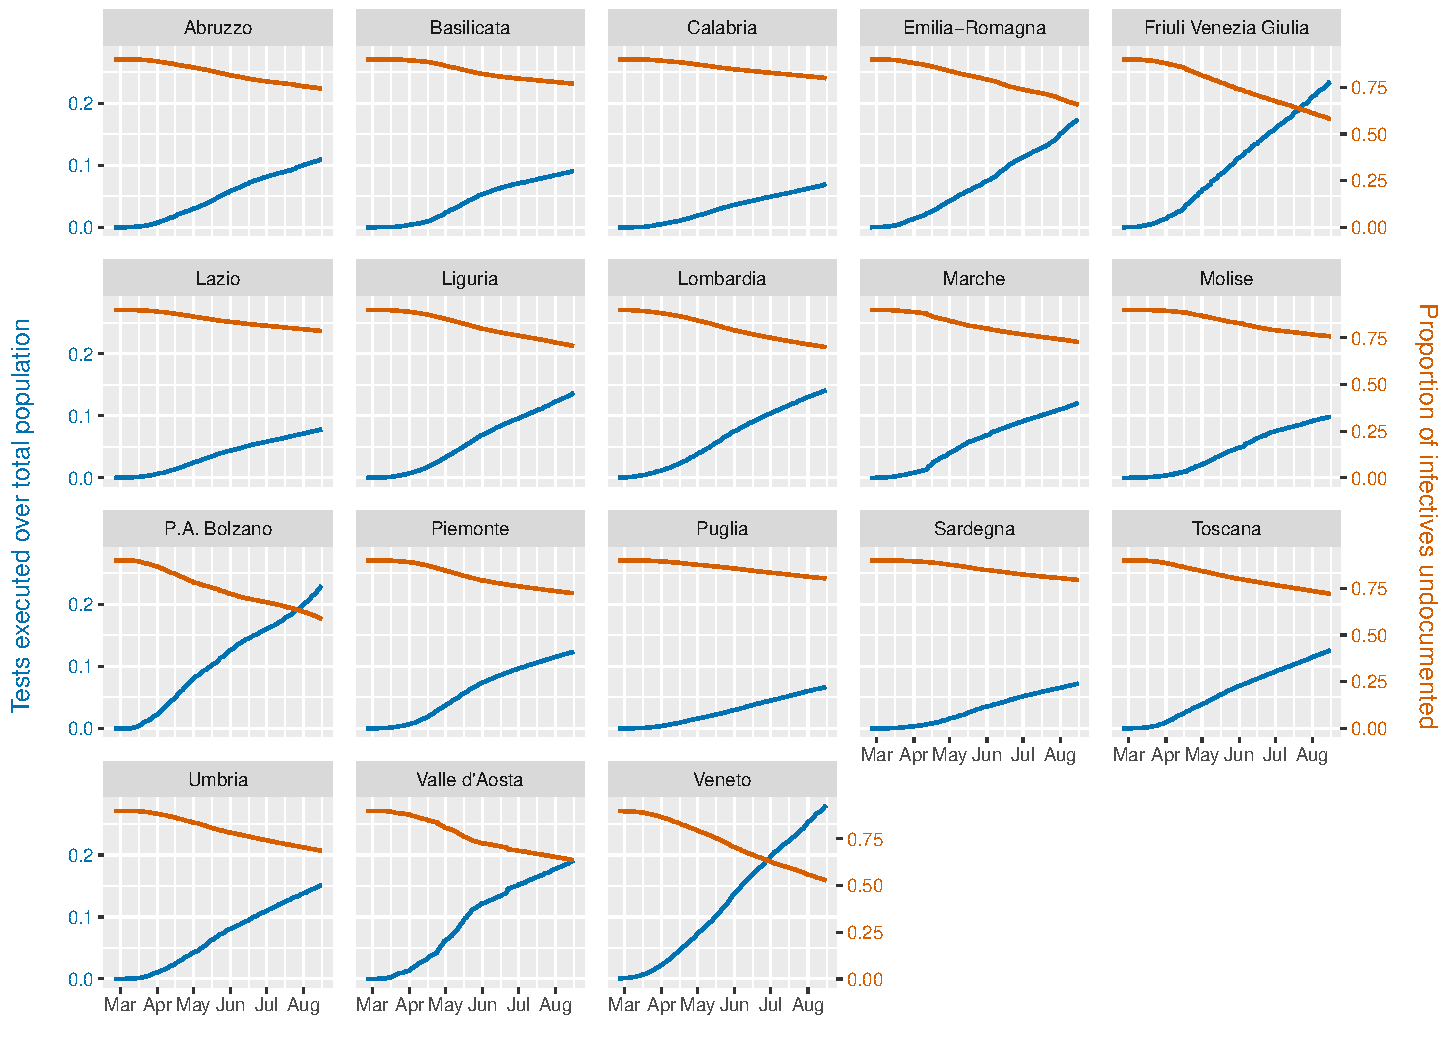
\includegraphics[width=\textwidth]{output/tamponiprop_vs_ft.pdf}
	    \caption{Total number of people tested over the total population ($TC_{p,t} / N_{p,t}$) versus proportion of infectives that are documented $f_{p,t}(\gamma)$. Undocumented infectives are modelled using the quadratic specification with $\gamma = 0.7$ and $f^{min}=0.1$.}
	    \label{fig:tamponiprop_versus_ft}
	\end{figure}
	
	To illustrate the impact of this modelling method, we give an example for three regions in Table \ref{tab:f_t_over_time}. We show the number of documented infectives $D_{r,t}$, the proportion of infectives that are documented $f_{r,t}$, and the resulting total number of infectives $i_{r,t}$, which is computed as $D_{r,t} / f_{r,t}$. For the three regions, we choose Calabria, Lombardy, and Veneto because these vary in the proportional amount of tests executed, leading to different profiles in $f_t$, as can be seen in Figure \ref{fig:tamponiprop_versus_ft}.
	
	\begin{table}[H]
		\centering
		\caption{Impact of modelling undocumented infectives over time. Undocumented infectives are modelled using the quadratic specification with $\gamma = 0.7$ and $f^{min}=0.1$.}
		\label{tab:f_t_over_time}
		\begin{tabular}{llllllllllll}
		    \toprule 
                     & \multicolumn{3}{c}{Calabria} && \multicolumn{3}{c}{Lombardy} && \multicolumn{3}{c}{Veneto} \\
                     \cmidrule{2-4}\cmidrule{6-8}\cmidrule{10-12}
                     & $D_{r,t}$  & $f_{r,t}$   & $i_{r,t}$   && $D_{r,t}$  & $f_{r,t}$   & $i_{r,t}$    && $D_{r,t}$  & $f_{r,t}$  & $i_{r,t}$   \\ \midrule
            April 1  & 669     & 10.8\%  & 6,448   && 44,601  & 11.8\%  & 409,003  && 9,592   & 13.4\% & 82,106  \\
            June 1   & 1,158   & 15.4\%  & 10,670  && 88,846  & 21.0\%  & 717,289  && 19,121  & 29.5\% & 139,610 \\
            August 1 & 1,269   & 19.2\%  & 11,291  && 96,102  & 28.5\%  & 747,691  && 20,133  & 44.2\% & 142,111 \\ \bottomrule
        \end{tabular}
	\end{table}
	
	Table \ref{tab:f_t_over_time} shows us that the impact of the proportion of documented infectives $f_t$ differs over the regions. When the amount of tests executed grows less steeply, as is the case in Calabria, the number of undocumented infectives in society grows stronger. On the other hand, for a region that invests heavily in testing, such as Veneto, the undocumented infectives are less pronounced. For example, consider the changes in Calabria and Veneto from June 1 to August 1. For Calabria, the growth in the documented infectives accounted for only 17.87\% of the total growth in infectives. In contrast, in Veneto the growth in the documented infectives accounted for 40.46\% of the total growth. Lombardy finds itself in the middle, where documented infectives make up 23.87\% of the total growth. Hence, our method correctly incorporates the intuition that a higher testing capacity leads to more infectives being documented.
	
	\section{Within-Region Spread Model} \label{sec:model_within}
	In this section, we present the within-region spread model as presented by \textcite{adda2016economic}, which ignores effects across regions. Section \ref{subsec:model_within_methodology} discusses the methodology, including the derivation of the model from the SIR model, moment conditions, and the inclusion of undocumented infectives. Subsequently, the results are presented in \ref{subsec:model_within_results}, where we discuss the statistical evidence, the magnitude of the estimates, and how they compare across the regions. Moreover, we investigate the progression of the estimates over time.
	
	\subsection{Methodology} \label{subsec:model_within_methodology}
	In this section, we present the methodology of the within-region spread model. Recall that the SIR model is postulated in continuous time. \textcite{adda2016economic} provides a discrete-time model that is based on the SIR model. \textcite{adda2016economic} does not discuss how the discretization is carried out. Therefore, we discuss how the discretization appears to be carried out. Recall from \eqref{eq:SIR_model_I} that $\frac{dI}{dt} = \beta SI - \gamma I$. As such, the discretized version (for a region $p$) for a single time period, without numerical integration, is:
	    \begin{equation}\label{eq:discretized_sir}
	        I_{p,t} - I_{p,t-1} = \beta S_{p,t-1}I_{p,t-1} - \gamma I_{p,t-1}.
	    \end{equation}
	   
	There are a few things to notice. Firstly, because a model is never fully able to represent reality, we need to account for statistical errors when estimating the parameters in \eqref{eq:discretized_sir}. This is incorporated in the model through an error term, denoted by $\eta_{p,t}$.
	    \begin{equation}\label{eq:discretized_sir_error}
	        I_{p,t} - I_{p,t-1} = \beta S_{p,t-1}I_{p,t-1} - \gamma I_{p,t-1} + \eta_{p,t}.
	    \end{equation}
	
	Secondly, individuals that get infected do not immediately infect others because there is a so-called latent period, which is the period between an infection and the moment that the infective is infectious. For COVID-19, the latent period is estimated to be approximately 2 days shorter than the incubation period \parencite{he2020temporal}. The incubation period is the period between an infection and the moment that the infected individual starts showing symptoms, at which point the infective is said to be symptomatic. The incubation period for COVID-19 is estimated to be above 2 and below 11.5 \parencite{lauer2020incubation}, 12.5 \parencite{li2020incubation}, or 14 days \parencite{linton2020incubation}. This is a large range, but this is not rare. For instance, the incubation period for chickenpox is estimated to be between 9 and 21 days \parencite{papadopoulos2018chickenpox}. While the maximum incubation period is not agreed upon by \textcite{lauer2020incubation} and \textcite{li2020incubation}, their results on the median are similar. \textcite{lauer2020incubation} report a median incubation period of 5.1 days (95\% CI: 4.5 to 5.8 days), while \textcite{li2020incubation} report a median incubation period of 5.2 days (95\% CI: 4.1 to 7.0 days). \textcite{linton2020incubation} do not report the median incubation period but instead give the result of a mean incubation period of 5.0 days (95\% CI: 4.2 to 6.0 days) when excluding Wuhan residents and 5.6 days (95\% CI: 5.0 to 6.3 days) when including Wuhan residents. \\
	
	Because the latent period is estimated to be shorter than the incubation period, there are infectives who are able to infect others before showing symptoms. We call these people pre-symptomatic, which is distinctive from asymptomatic people in the sense that asymptomatic people do not develop symptoms while pre-symptomatic people will develop symptoms. A key characteristic of pre-symptomatic people is that they develop a higher viral load just before said symptoms become apparent. On June 9, 2020, the World Health Organization said that pre-symptomatic people may actually be able to infect others \parencite{bloomberg2020AsymptomaticSpread}. This may be an issue when considering policies such as self-isolation when one is sick, because an infective may have already spread the virus before feeling sick. \textcite{bloomberg2020AsymptomaticSpread} moreover reiterate the WHO's statement that studies have been done that show that asymptomatic people can spread the virus but that more research needs to be done to show how many of these infectious asymptomatic people exist. We discussed how we model pre-symptomatic individuals in the form of undocumented infectives in Section \ref{sec:undocumented_modelling}. \\
	
	\textcite{adda2016economic} models the transmission lag by making the lag on the right hand side of \eqref{eq:discretized_sir_error} dependent on the incubation period. This is denoted by the parameter $\tau$:
	    \begin{equation}\label{eq:discretized_sir_tau}
	        I_{p,t} - I_{p,t-1} = \beta S_{p,t-\tau}I_{p,t-\tau} - \gamma I_{p,t-1} + \eta_{p,t}.
	    \end{equation}
	
	Note that we have not included the lag $\tau$ in the term $\gamma I_{p,t-1}$, which represents the recovery rate. This is because when a person recovers from the disease, they immediately move to that group and this is independent of the incubation period. \textcite{adda2016economic} chooses $\tau$ equal to one week for acute diarrhea and flu-like illnesses as these have an incubation period of less than a week. A value of $\tau$ equal to 3 weeks is chosen for chickenpox. Due to the results from \textcite{lauer2020incubation}, \textcite{li2020incubation}, and \textcite{linton2020incubation}, indicating an incubation period for COVID-19 of at most 14 days, we choose $\tau = 14$. \\
	
	\textcite{adda2016economic} adds regressors to the model as control variables, such as the region fixed effects, week effects and year effects in levels. Regressors can be added to the model to capture possible effects that would otherwise be included in the error, confounding the estimation of the transmission parameter $\beta$. \textcite{adda2016economic} denotes this tensor of regressors by $X$. This leads to the following formulation:
	    \begin{equation}\label{eq:discretized_sir_regressors}
        	I_{p,t} - I_{p,t-1} = \beta S_{p,t-\tau}I_{p,t-\tau} - \gamma I_{p,t-1} + \delta X_{p,t} + \eta_{p,t}.
    	\end{equation}
    	
	For our application, the data does not span multiple years. As such, we do not have year effects. Also note that week effects would capture a time trend because we do not have the same week number multiple times for the same region. Therefore, we do not include a week effect. We do add a weekend effect. More information and reasoning is provided in Section \ref{subsec:regressor_data}. \\
	
	There are two other key differences in the model specification by \textcite{adda2016economic} compared to \eqref{eq:discretized_sir_regressors} that are not clearly motivated in their paper. First of all, \textcite{adda2016economic} replaces the incidence rate $I_{p,t-\tau}$ by the number of new cases $i_{p,t-\tau} - i_{p,t-\tau-1}$ and uses the number of new cases $i_{p,t} - i_{p,t-1}$ as the dependent variable instead of $I_{p,t} - I_{p,t-1}$. Second of all, \textcite{adda2016economic} does not include the term $\gamma I_{p,t-1}$ in the model. Presumably, this is because \textcite{adda2016economic} considers the number of new cases instead of the total number of infectives and, therefore, the number of recovered individuals do not impact that value. In this section and Section \ref{subsec:model_between_methodology}, we continue with this model to see how the models perform in the case of COVID-19. Even though the mathematical derivation of the model does not explicitly derive from the SIR model, it may still provide correct estimates although there is no econometric evidence for this so far. \\
	
	Now we present the final model, ignoring effects across regions, by \textcite{adda2016economic}. Defining $\Delta i_{p,t} \coloneqq i_{p,t} - i_{p,t-1}$, the within-region spread model is given by:
	\begin{equation} \label{eq:model_within}
	    \Delta i_{p,t} = \beta_{within}S_{p,t-\tau}\Delta i_{p,t-\tau} + \delta X_{p,t} + \eta_{p,t}.
	\end{equation}
	
	One could naively consider constructing a model for the entire nation of Italy. Even though this does not take into account regional differences, as described in Section \ref{sec:problem_description}, it may achieve good results if regions are sufficiently similar. For good measure, we also estimate a national model. This is done in two ways, the first of which is simply by adding the values of $s$, $i$, and $r$ of all regions together to obtain the national numbers, for which the model from \eqref{eq:model_within} or \eqref{eq:model_within_undocumented}, depending on whether undocumented infectives are modelled, is estimated. The results from this model will be labelled with National (OLS) in Section \ref{subsec:model_within_results}. The second method is to apply pooled OLS (POLS), which is a panel data estimation method. This model ignores the individual regional effect, hence treating the data as one large cross-section. This means that the $T$ observations for some region $p$ are actually treated to be cross-sectional observations of $T$ different individuals. These results will be labelled with National (POLS) in Section \ref{subsec:model_within_results}. \\
	
	The model in \ref{eq:model_within} is estimated by ordinary least squares (OLS). The moment condition that needs to be satisfied due to the strict exogeneity assumption is:
	    \[E\left[ \eta_{p,t} \left( \beta_{within}S_{p,t-\tau}\Delta i_{p,t-\tau} + \delta X_{p,t} \right) \right] = 0.\]
	
	A general assumption that is made, is that the idiosyncratic error $\eta_{p,t}$ is uncorrelated with the regressors in the tensor $X_{p,t}$. Therefore, we assume that $E\left[\eta_{p,t} \,\middle|\, X_{p,t}\right] = 0$. The reason why we assume that $E\left[\eta_{p,t} \,\middle|\, S_{p,t-\tau}\Delta i_{p,t-\tau}\right] = 0$ is that, for a large enough lag $\tau$, the error is not correlated with past data at that lag. By that, we mean that the people that are classified as infectives at time $t-\tau$ do not have an effect on the error that we make when considering the infectives at time $t$ under a correct model specification. Because we chose $\tau$ to exceed the maximum estimated incubation period, we assume that this holds. Therefore, we assume that the moment condition holds. \\
	
	Using the specification of undocumented infectives, we can now adapt the model to include these undocumented infectives. Using that $\Delta i_{p,t} = \frac{D_{p,t}}{f_{p,t}(\gamma)} - \frac{D_{p,t-1}}{f_{p,t-1}(\gamma)}$, the model in \eqref{eq:model_within} becomes:
	
	    \begin{equation} \label{eq:model_within_undocumented}
		    \frac{D_{p,t}}{f_{p,t}(\gamma)} - \frac{D_{p,t-1}}{f_{p,t-1}(\gamma)} = \beta_{within}S_{p,t-\tau}\left(\frac{D_{p,t-\tau}}{f_{p,t-\tau}(\gamma)} - \frac{D_{p,t-\tau-1}}{f_{p,t-\tau-1}(\gamma)}\right) + \delta X_{p,t} + \eta_{p,t}.
	    \end{equation}
	    
	\noindent We can rewrite \eqref{eq:model_within_undocumented} as follows
	    \begin{equation*}
	       D_{p,t} = f_{p,t}(\gamma)\left(\beta_{within}S_{p,t-\tau}\left(\frac{D_{p,t-\tau}}{f_{p,t-\tau}(\gamma)} - \frac{D_{p,t-\tau-1}}{f_{p,t-\tau-1}(\gamma)}\right) + \frac{D_{p,t-1}}{f_{p,t-1}(\gamma)} + \delta X_{p,t} + \eta_{p,t}\right).
	    \end{equation*}
	    
	\noindent The moment conditions that then need to hold are:
	    \begin{align*}
	        & E\left[ \eta_{p,t}f_{p,t}(\gamma) \left( \beta_{within}S_{p,t-\tau}\left(\frac{D_{p,t-\tau}}{f_{p,t-\tau}(\gamma)} - \frac{D_{p,t-\tau-1}}{f_{p,t-\tau-1}(\gamma)}\right) + \frac{D_{p,t-1}}{f_{p,t-1}(\gamma)} + \delta X_{p,t} \right) \right] = 0 \\
	        \iff & f_{p,t}(\gamma) E\left[ \eta_{p,t}\left( \beta_{within}S_{p,t-\tau}\left(\frac{D_{p,t-\tau}}{f_{p,t-\tau}(\gamma)} - \frac{D_{p,t-\tau-1}}{f_{p,t-\tau-1}(\gamma)}\right) + \frac{D_{p,t-1}}{f_{p,t-1}(\gamma)} + \delta X_{p,t} \right) \right] = 0.
	    \end{align*}
	
	Since $f_{p,t}(\gamma)$ is simply a scaling function, regardless of the chosen parameter, it has no influence on the dependence between the error and the regressors. As such, it can be taken out of the expectation term. Subsequently, we can divide both sides of the equation by $f_{p,t}(\gamma)$ to obtain the following moment condition:
	    \begin{equation} \label{eq:model_within_undocumented_moments}
	        E\left[ \eta_{p,t}\left( \beta_{within}S_{p,t-\tau}\left(\frac{D_{p,t-\tau}}{f_{p,t-\tau}(\gamma)} - \frac{D_{p,t-\tau-1}}{f_{p,t-\tau-1}(\gamma)}\right) + \frac{D_{p,t-1}}{f_{p,t-1}(\gamma)} + \delta X_{p,t} \right) \right] = 0.
	    \end{equation}
	
	Just like earlier in this section, we make the assumption that the idiosyncratic error $\eta_{p,t}$ is uncorrelated with the regressors in the tensor $X_{p,t}$. Therefore, we assume that $E\left[\eta_{p,t} \,\middle|\, X_{p,t}\right] = 0$. We assume that $E\left[\eta_{p,t} ~\middle|\, S_{p,t-\tau}\left(\frac{D_{p,t-\tau}}{f_{p,t-\tau}(\gamma)} - \frac{D_{p,t-\tau-1}}{f_{p,t-\tau-1}(\gamma)}\right)\right] = 0$ for the same reason as earlier in this section, namely that for a large enough lag $\tau$, the error is not correlated with past data at that lag. This is independent of the scaling functions $f_{p,t-\tau}(\gamma)$ and $f_{p,t-\tau-1}(\gamma)$ as these are constructed without the past infectives in mind. \\
	
	Recall that the error $\eta_{p,t}$ is made when predicting the amount of infectives at time $t$. In Section \ref{subsec:model_within_methodology}, we have explained that there is a latent period during which an infected person is not able to infect others yet. As such, when considering only a one-period difference, there should be no correlation between $\eta_{p,t}$ and $D_{p,t-1}$. Moreover, as was explained in the previous paragraph, $\eta_{p,t}$ is independent of the scaling function $f_{p,t-1}(\gamma)$. Therefore, we can assume that $E\left[\eta_{p,t} \,\middle|\, \frac{D_{p,t-1}}{f_{p,t-1}(\gamma)}\right] = 0$. Consequently, the scaling of the infectives by using our functional form, has no additional impact on the moment conditions. Therefore, we assume that the moment conditions in \eqref{eq:model_within_undocumented_moments} hold, even when modelling undocumented infectives. \\
	
	To conclude this section, for all models, we use the last 100 days of data, which spans May 9 until August 16. The reason behind this is that infections from the past should not dominate the latest estimates of the transmission rate parameters. When the (first) wave has passed and the transmission rate is low, including the data from during the peak moment of the pandemic will influence the transmission rate. Consider Figure \ref{fig:beta_within_over_time_nordest_not_rolling}, where we present the plot of the estimated values of $\beta_{within}$ over time for the Nord-Est NUTS 1 region when all $T$ data points are used.
	
	\begin{figure}[H]
	    \centering
        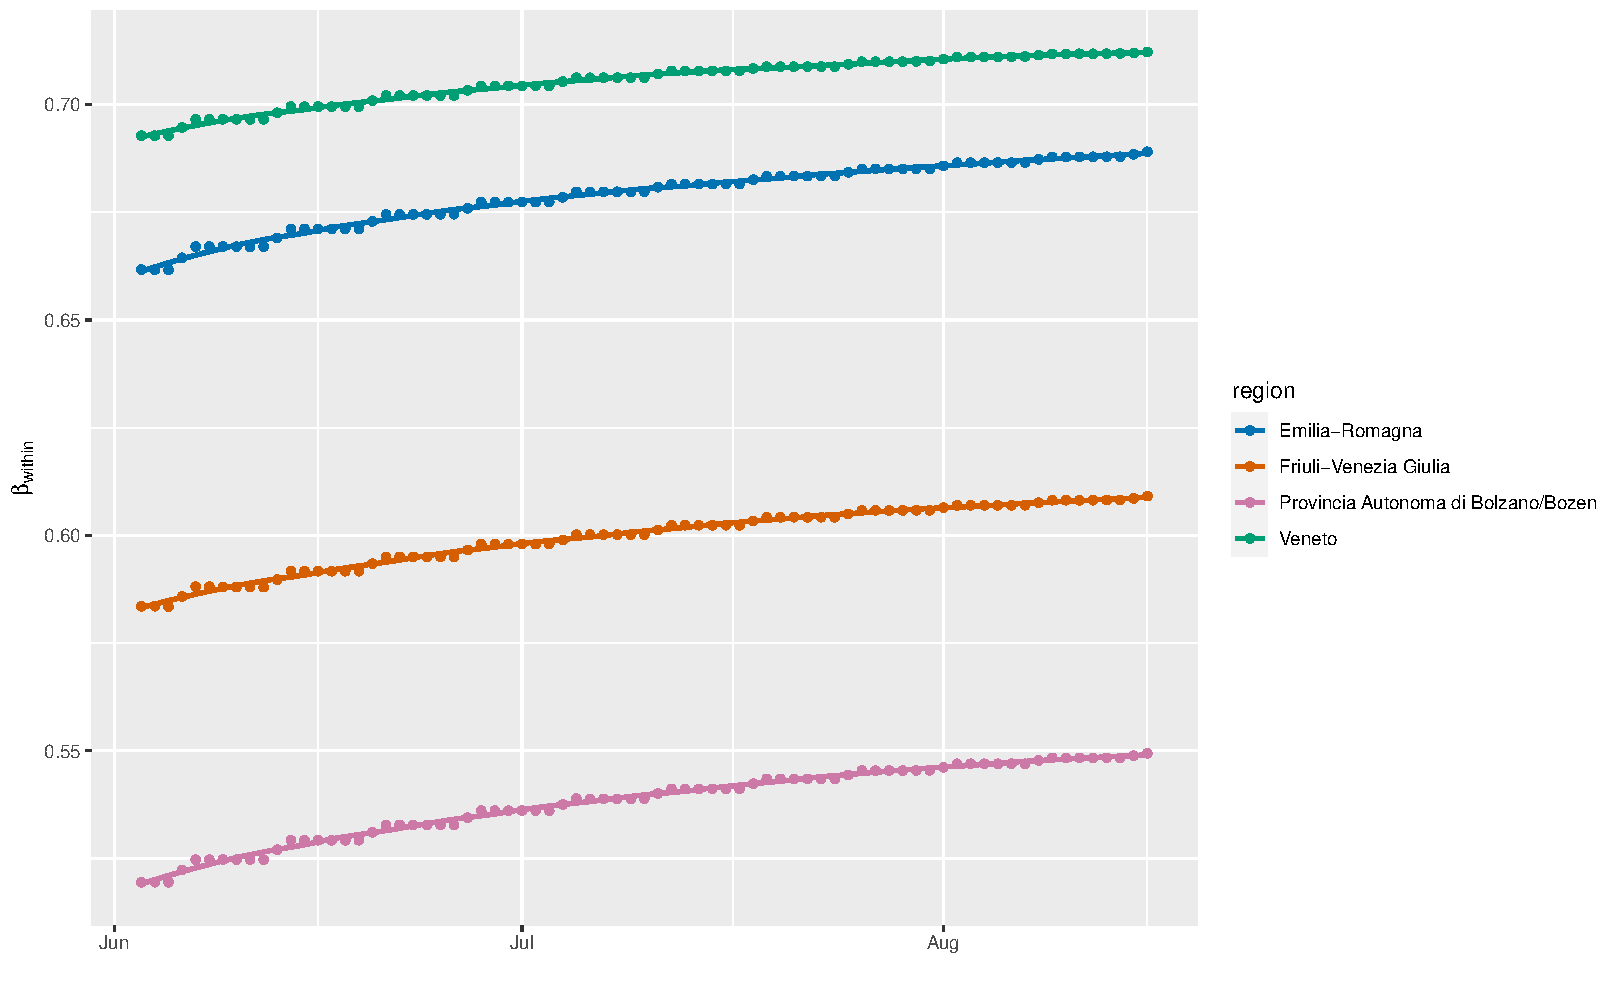
\includegraphics[width=0.92\linewidth]{output/model_within_lag14_betawithin_Nord-Est_UndocQuadratic.pdf}
	    \caption{Progression of $\beta_{within}$ over time for the Nord-Est NUTS 1 region using all $T$ data points. Undocumented infectives are modelled using the quadratic specification with $\gamma = 0.7$ and $f^{min}=0.1$.}
	    \label{fig:beta_within_over_time_nordest_not_rolling}
    \end{figure}
	
	It is immediately clear that the variation in $\beta_{within}$ is minimal and even slightly increasing. This not intuitive for the reason that a decrease in infectives over time would lead to a lower estimated transmission parameter. As such, it is not logical that the estimate for $\beta_{within}$ would level out, especially at a level not close to zero, or increase. The reason behind choosing 100 days is arbitrary, however; it is simply a number that retains enough data points while providing variation in the estimates for $\beta_{within}$.
	
    \subsection{Results} \label{subsec:model_within_results}
	In this section, we present the results for the within-region spread model. Firstly, we present the results where the data is pooled to a national level. Subsequently, results are presented for the models per region after applying model selection with the Akaike Information Criterion (AIC). For both result sets, we present the results from the regular model as well as modelling the undocumented infectives with a quadratic form with $\gamma = 0.7$ and $f^{min} = 0.1$ as in \eqref{eq:quadratic_functional_form}. If no statistical significance level is mentioned, we take a significance level of 0.05. \\
	
	The results from estimating a national-level model, as mentioned at the end of the previous section, are given in Table \ref{tab:results_within_national}. Model selection with AIC is not applied and undocumented infectives are not included.
	
	\begin{table}[H]
	    \centering
	    \caption{Estimates from the within-region spread model on a national level. Data spans May 9 until August 16, 2020 (100 days). Undocumented infectives are not modelled.}
		\label{tab:results_within_national}
	    \begin{tabular}{lrrrlrrrl}
	        \toprule
    		& \multicolumn{4}{c}{OLS} & \multicolumn{4}{c}{Pooled OLS} \\
    		                \cmidrule(lr){2-5}
                            \cmidrule(lr){6-9}
    		& Estimate & Std. Error & $t$-value & $p$-value & Estimate & Std. Error & $t$-value & $p$-value \\* \midrule
    		Weekend             & 92.860 & 30.241 & 3.071 & 0.003*** & 15.086 & 2.974 & 5.074 & 0.000*** \\*
    		$\beta_{within}$    & 0.493 & 0.022 & 21.992 & 0.000*** & 0.533 & 0.019 & 27.980 & 0.000*** \\* \bottomrule
    		\multicolumn{9}{c}{Significance levels: * = 0.1 ** = 0.05, *** = 0.01}
	    \end{tabular}
	\end{table}
	
	Table \ref{tab:results_within_national} shows estimates for $\beta_{within}$, denoted by $\hat{\beta}_{within}$, of 0.493 and 0.533 for the national model estimated by OLS and POLS, respectively. Both estimated parameters are statistically significant at a 1\% significance level. This seems to imply that the POLS model estimates that the transmission is a bit worse than the OLS model estimates. We apply a $t$-test to test whether these estimates are statistically different from one another. The null hypothesis is given by:
	    \[H_0:~ \beta_{within, OLS} - \beta_{within,POLS} = 0.\]
	The test statistic is constructed as follows:
	    \[t = \frac{\hat{\beta}_{within, OLS} - \hat{\beta}_{within, POLS}}{\sqrt{s.e.^2_{within, OLS} - s.e.^2_{within, POLS}}},\]
	where $s.e.$ represents the standard error. If we fill out the needed values, we find that $t = -1.376$. Since the absolute value of $t$ does not exceed the critical value $t_{T; 0.95} = 1.96$, we do not find statistical evidence in favour of the null hypothesis, at a significance level of 0.05, and we cannot say that the methods lead to different results. \\
	
	As mentioned at the end of the previous section, this national model does not take into account effects specific to regions. It is also clear that the same model might not be suitable for all regions; we should apply model selection to the individual models as was explained in Section \ref{sec:model_selection}. To execute model selection, we use the AIC and we make sure that the term for $\beta_{within}$ remains in the model, meaning that model selection is solely performed on whether the weekend dummy should be included. In Table \ref{tab:results_within_aic}, we present the results. In Table \ref{tab:results_within_no_ms} in Appendix \ref{app:tables}, we present the results without applying model selection. The results comparing the use of the BIC over the AIC for model selection are presented in Table \ref{tab:model_within_aic_vs_bic}.
	
	% This makes the `longtables` (throughout the document) centered on the page (exceeding both margins.
	\setlength{\LTleft}{-20cm plus -1fill}
    \setlength{\LTright}{\LTleft}
	
	\begin{longtable}{@{}lcccc@{}}
		\caption{Estimates from the within-region spread model per region with model selection by AIC. Estimates are given with $t$-statistics in parentheses. Data spans May 9 until August 16, 2020 (100 days). Undocumented infectives are modelled using the quadratic specification with $\gamma = 0.7$ and $f^{min}=0.1$.}
		\label{tab:results_within_aic}\\
		\toprule
		                & \multicolumn{2}{c}{Regular model} & \multicolumn{2}{c}{Modelling undocumented infectives} \\
		                \cmidrule(lr){2-3}
                        \cmidrule(lr){4-5}
		Region          & $\beta_{within}$ & Weekend & $\beta_{within}$ & Weekend \\* \midrule
		\endfirsthead
		
		\multicolumn{5}{c}{{\bfseries Table \thetable\ continued from previous page}} \\
		\toprule
		                & \multicolumn{2}{c}{Regular model} & \multicolumn{2}{c}{Modelling undocumented infectives} \\
		                \cmidrule(lr){2-3}
                        \cmidrule(lr){4-5}
		Region          & $\beta_{within}$ & Weekend & $\beta_{within}$ & Weekend \\* \midrule
		\endhead
		
		\bottomrule
		\multicolumn{5}{c}{{\bfseries Table \thetable\ continues on next page}}
		\endfoot
		
		\multicolumn{5}{c}{Significance levels: * = 0.1 ** = 0.05, *** = 0.01}
		\endlastfoot
		
        National (OLS) & 0.493*** & 92.860*** & 0.423*** & 379.483*** \\ 
         & (21.992) & (3.071) & (27.417) & (2.976) \\ 
        National (POLS) & 0.533*** & 15.086*** & 0.458*** & 90.994*** \\ 
         & (27.980) & (5.074) & (22.981) & (4.893) \\ 
        Abruzzo & 0.372*** & 2.751** & 0.322*** & 13.454** \\ 
         & (4.952) & (2.091) & (6.253) & (2.249) \\ 
        Basilicata & 0.073 &  & 0.077 &  \\ 
         & (0.665) &  & (0.764) &  \\ 
        P.A. Bolzano & 0.269*** & 2.346*** & 0.219*** & 7.117*** \\ 
         & (3.468) & (3.683) & (4.175) & (3.961) \\ 
        Calabria & 0.242** & 2.189** & 0.201* & 12.897*** \\ 
         & (2.043) & (2.614) & (1.917) & (2.828) \\ 
        Emilia-Romagna & 0.358*** & 22.416*** & 0.287*** & 91.467*** \\ 
         & (11.673) & (4.844) & (14.768) & (5.266) \\ 
        Friuli Venezia Giulia & 0.342*** & 2.582*** & 0.252*** & 8.578*** \\ 
         & (7.559) & (3.476) & (8.891) & (3.508) \\ 
        Lazio & 0.494*** & 10.172*** & 0.424*** & 57.018*** \\ 
         & (10.069) & (3.441) & (11.273) & (3.610) \\ 
        Liguria & 0.382*** & 4.179 & 0.332*** &  \\ 
         & (11.931) & (1.430) & (14.770) &  \\ 
        Lombardy & 0.583*** &  & 0.513*** &  \\ 
         & (18.205) &  & (18.615) &  \\ 
        Marche & 0.436*** & 2.697** & 0.387*** & 12.796** \\ 
         & (9.376) & (2.144) & (11.347) & (2.286) \\ 
        Molise & 0.140 & 1.855** & 0.155* & 11.448** \\ 
         & (1.595) & (2.456) & (1.810) & (2.299) \\ 
        Piedmont & 0.352*** & 7.449* & 0.300*** & 28.533 \\ 
         & (23.006) & (1.896) & (25.913) & (1.492) \\ 
        Apulia & 0.376*** & 3.804** & 0.335*** & 23.618*** \\ 
         & (6.165) & (2.581) & (7.302) & (2.719) \\ 
        Sardinia & 0.437*** &  & 0.276*** & 5.301 \\ 
         & (4.417) &  & (3.874) & (1.655) \\ 
        Tuscany & 0.281*** & 8.444*** & 0.237*** & 35.079*** \\ 
         & (6.666) & (3.854) & (8.744) & (3.929) \\ 
        Umbria & 0.436*** & 1.428*** & 0.291*** & 5.402*** \\ 
         & (3.936) & (3.168) & (4.134) & (3.351) \\ 
        Aosta Valley & 0.290*** &  & 0.302*** &  \\ 
         & (4.341) &  & (6.394) &  \\ 
        Veneto & 0.489*** & 11.951* & 0.284*** & 39.380*** \\ 
         & (6.748) & (1.920) & (7.344) & (2.672) \\* \bottomrule
	\end{longtable}

    We first discuss the statistical evidence for the estimated values of $\beta_{within}$, where we start by considering the model excluding undocumented infectives. After this, we consider the interpretation of the coefficients and the model selection. Considering the estimates of $\beta_{within}$, we see that these differ vastly over the regions with varying degrees of statistical significance. For only two regions, we find no statistically significant result, namely Basilicata and Molise. This may be due to not enough regional variation but the results may still be significant for policy purposes even if they are not statistically significant. For the region of Calabria, the estimate of $\beta_{within}$ is statistically significant at a significance level of 0.05. For all other regions, the estimates are statistically significant at a significance level of 0.01. Looking only at the statistically significant estimates, these range from 0.242 for Calabria until 0.583 for Lombardy. This already shows that a national model should not be applied to individual regions, despite the statistical significance of the estimates of $\beta_{within}$ for the national models. \\

    If we model undocumented infectives, we again see that no statistical evidence is found for a nonzero transmission rate for Basilicata and Molise, although the latter is now significant at a significance level of 0.1. Moreover, the estimate for Calabria is not significant anymore at a significance level of 0.05. For all other regions, the estimate is statistically significant at a significance level of 0.01, ranging from 0.219 for Bolzano until 0.513 for Lombardy. Notice that modelling undocumented infectives does not seem to impact the order of magnitude between the regions. For instance, where Lazio has the second-highest estimate for the case when undocumented infectives are not modelled, excluding the national models, it retains that position when undocumented infectives are included. Moreover, notice that the estimates for all regions, excluding the statistically insignificant ones, are all lower. Therefore, it appears that modelling undocumented infectives tends to decrease the estimates of the within-region transmission rate $\beta_{within}$. \\

    We are again interested in investigating whether the differences in the estimates differ significantly. For this, recall that the standard error of the estimate can be computed by dividing the estimate by the $t$-statistic. The $t$-statistic for the national models are equal to 2.572 (OLS) and 2.720 (POLS), thereby exceeding the critical value $t_{T;0.95} = 1.96$ and indicating that modelling undocumented infectives yields statistically different results at a significance level of 0.05. Besides the national models, there is only one other region for which the estimates differ significantly, namely Veneto, which has a $t$-statistic of 2.496. It is noteworthy to mention that the region of Emilia-Romagna has a $t$-statistic of 1.955, thereby barely not exceeding the critical value. With this $t$-statistic, the estimates are statistically significant different at a significance level of 5.06\%. This can be computed by using the density function of the Student's $t$-distribution. \\

    When we want to interpret the estimates of $\beta_{within}$, we should recall that \textcite{adda2016economic} notices that these can be interpreted as the marginal effects of a change in the infection rate on the future infection rate when the entire population is susceptible to the disease. However, notice that this is made with the model formulation as explained in Section \ref{subsec:model_within_methodology}, where the removal term is omitted from the model. Because this does not take into account the specific removal rate of COVID-19, we cannot interpret the coefficients in the same way. However, we can compare the magnitude of the coefficients with one another. For instance, let us compare the regions of Lombardy and the island of Sardinia. We consider the model where undocumented infectives are modelled. For this model, we find estimates of $\beta_{within}$ of 0.513 and 0.276, respectively. Although this cannot tell us much about the spread within the region as explicitly, this does show us that the transmission in Lombardy was much more severe than on Sardinia. A similar interpretation can be applied to any comparison of regions and for the model without modelling undocumented infectives. \\

    Regarding the model selection, we indeed see that the AIC gives a varying model selection per region. However, the set of regressors that is used is generally the same whether undocumented infectives are modelled are not. The only two exceptions that we see are for the region of Liguria and the island of Sardinia. When excluding undocumented infectives, the weekend dummy is included in the model for Liguria, whereas it is excluded when undocumented infectives are modelled. For Sardinia, it is the other way around. We do see that some of the estimates for the weekend dummy's parameter are not statistically significant at a significance level of 0.05. As mentioned in Section \ref{sec:model_selection}, this is because the AIC tends to select a larger model. Regardless of whether undocumented infectives are included or not, the entire model is selected for sixteen out of twenty models, and, in the other four cases, the weekend dummy is excluded. \\
	
	We are also interested in looking at the estimate of $\beta_{within}$ over time. We expect that it decreases over time, implying that SARS-CoV-2 is transmitted less. In Figure \ref{fig:beta_within_over_time_nordest}, we present plots for the regions in the Nord-Est NUTS 1 region. Plots for the other NUTS 1 regions can be found in Appendix \ref{sapp:figures_model_within}, which generally show similar results. Each point in the graphs in Figure \ref{fig:beta_within_over_time_nordest} is the estimate of $\beta_{within}$ when only the latest 100 data points before that date are used. In addition, a LOESS (locally estimated scatter plot smoothing) curve with span parameter 0.3 is fit to the data points. \\
	
	\begin{figure}[H]
	    \centering
	    \begin{subfigure}{\textwidth}
	      \centering
	      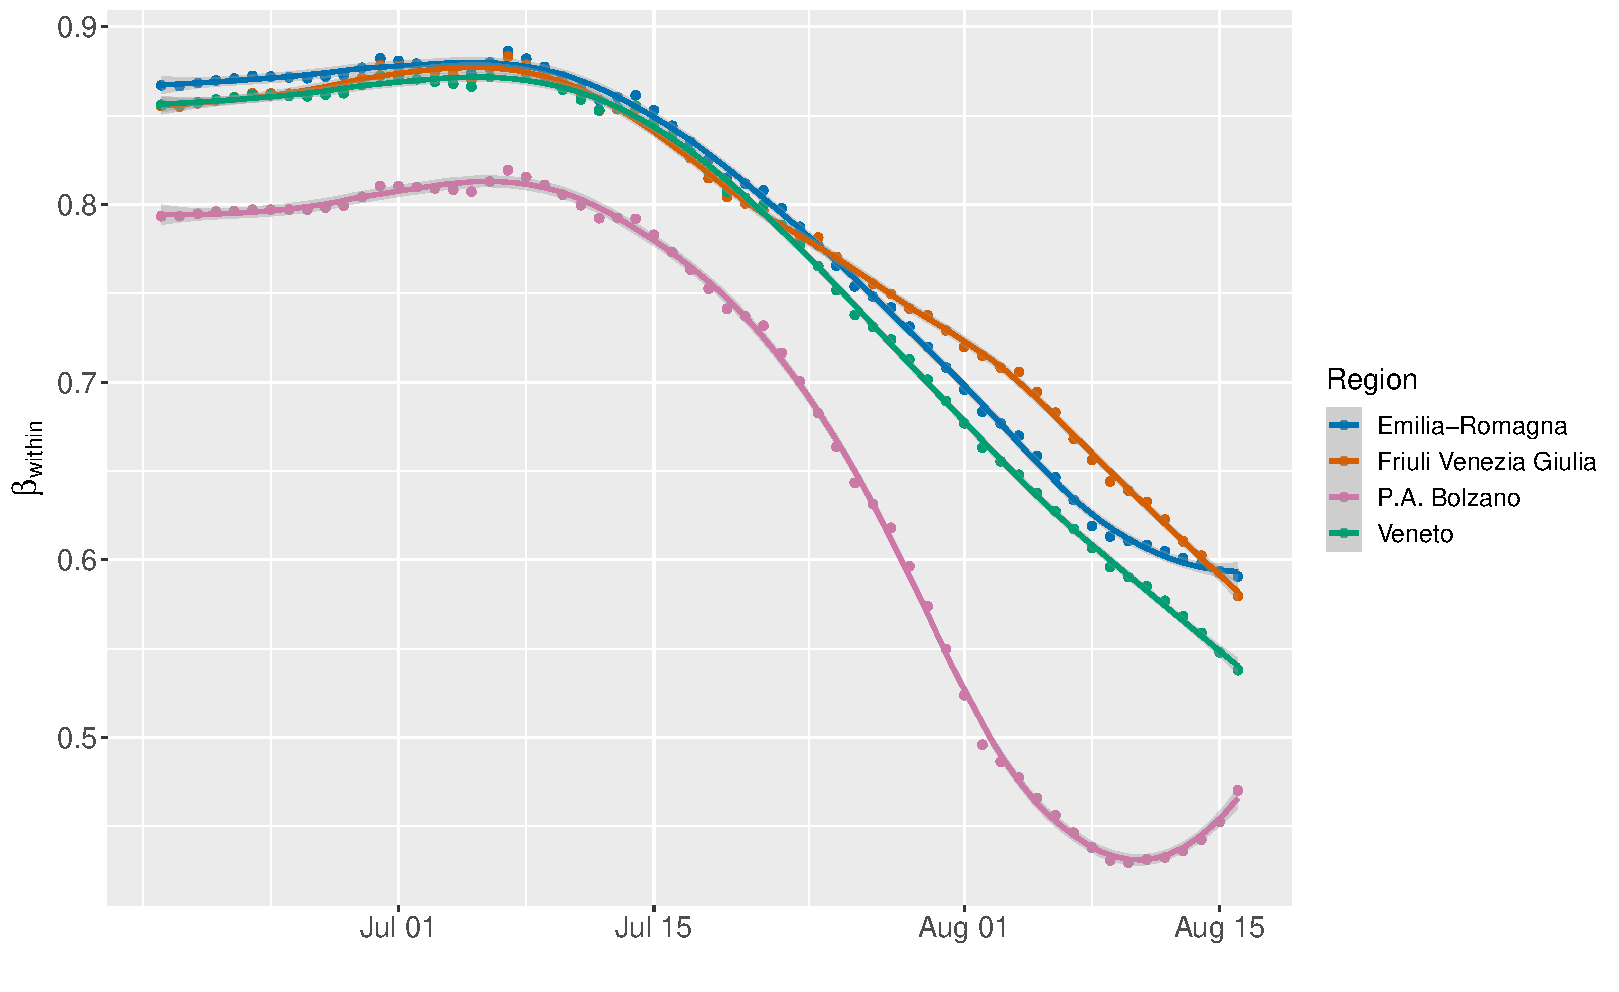
\includegraphics[width=0.92\linewidth]{output/model_within_lag14_betawithin_Nord-Est_rolling.pdf}
	      \caption{Without model selection}
	      \label{fig:beta_within_over_time_nordest_regular}
	    \end{subfigure}\newline
	    \begin{subfigure}{\textwidth}
	      \centering
	      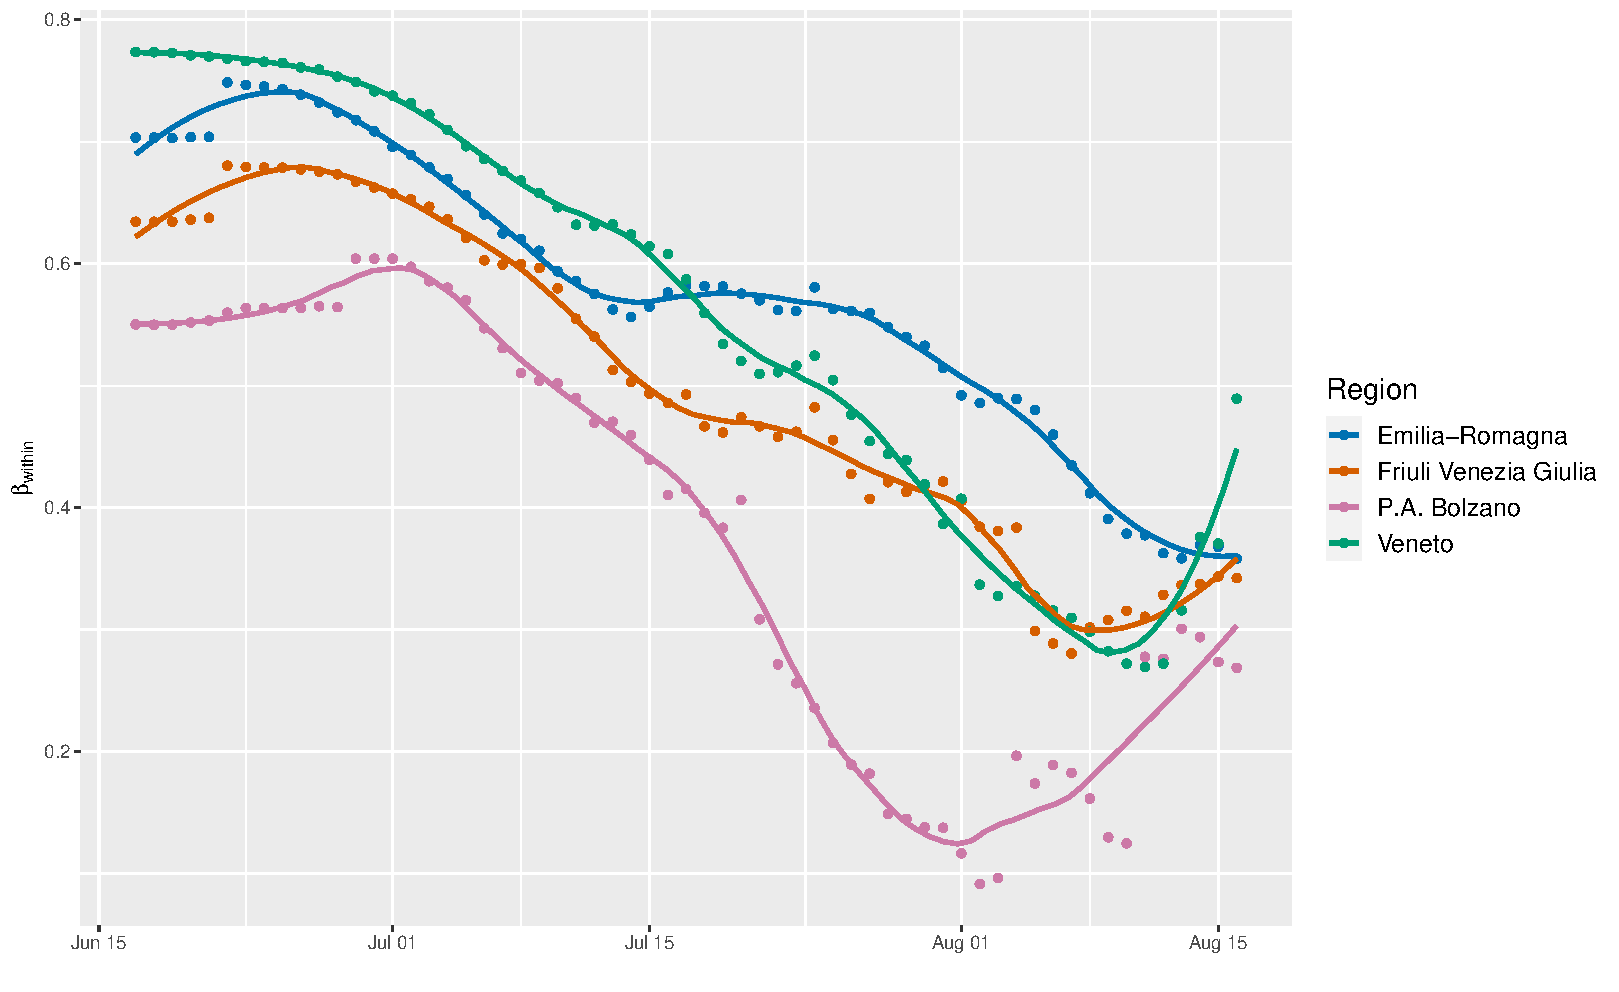
\includegraphics[width=0.92\linewidth]{output/model_within_lag14_betawithin_Nord-Est_aic_rolling.pdf}
	      \caption{With model selection by AIC}
	      \label{fig:beta_within_over_time_nordest_aic}
	    \end{subfigure}
	\end{figure}
    \begin{figure}[H]\ContinuedFloat
	    \begin{subfigure}{\textwidth}
	      \centering
	      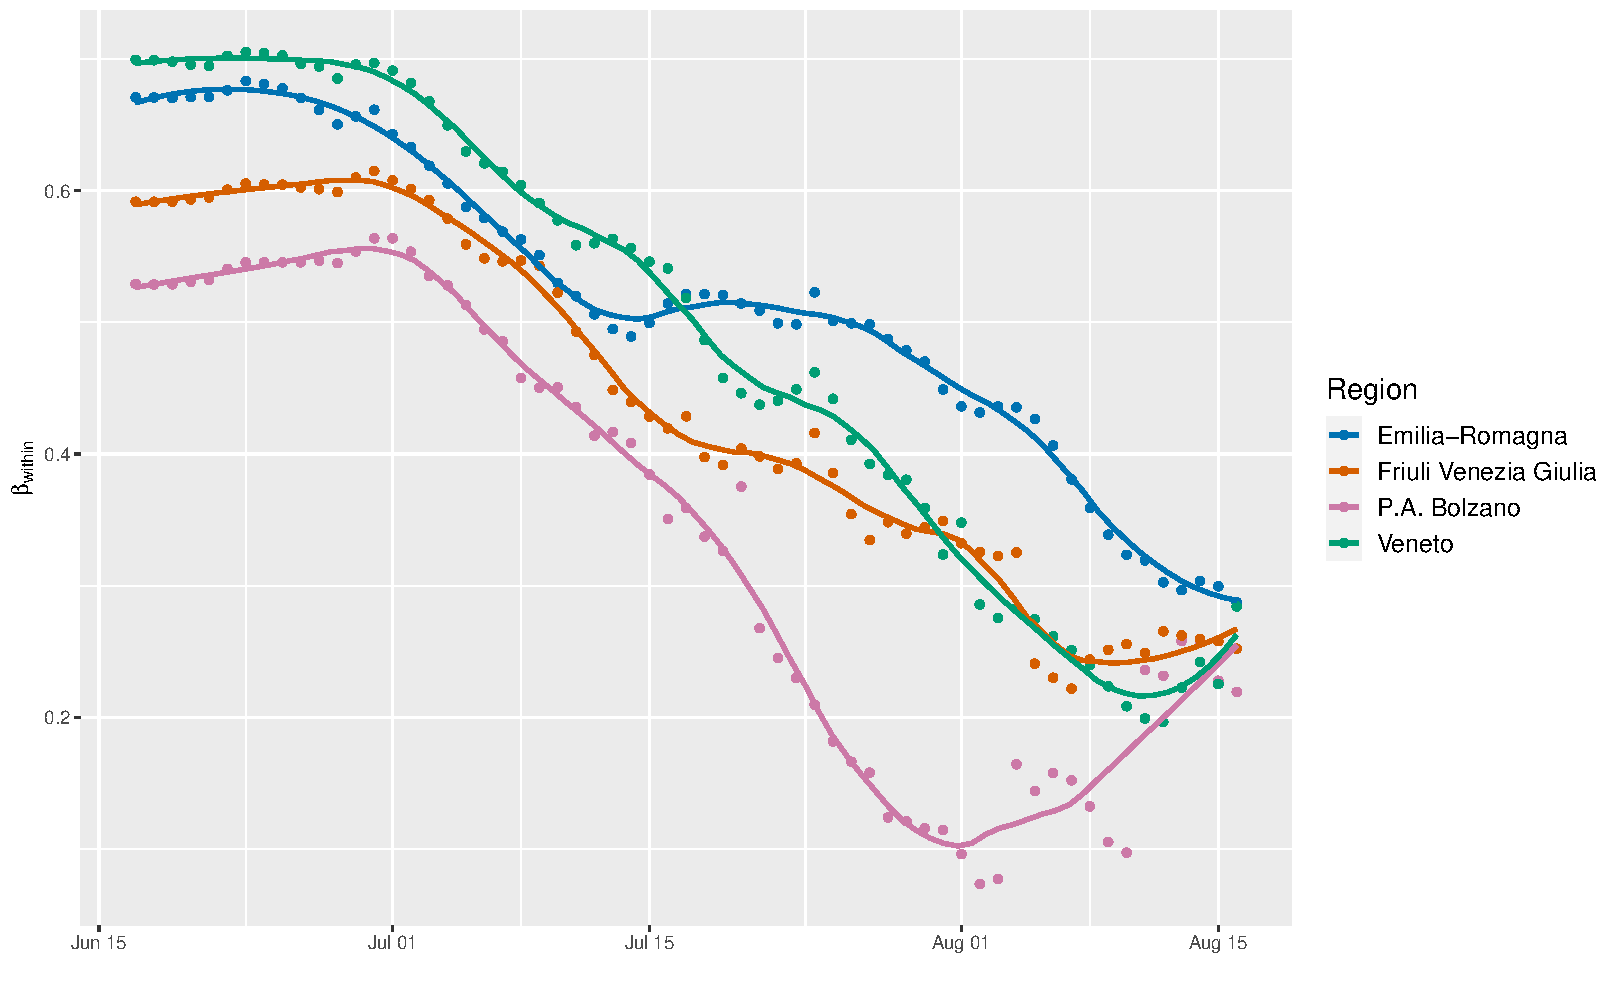
\includegraphics[width=0.92\linewidth]{output/model_within_lag14_betawithin_Nord-Est_UndocQuadratic_rolling.pdf}
	      \caption{Without model selection; \\ including undocumented infectives}
	      \label{fig:beta_within_over_time_nordest_regular_undoc}
	    \end{subfigure}\newline
	    \begin{subfigure}{\textwidth}
	      \centering
	      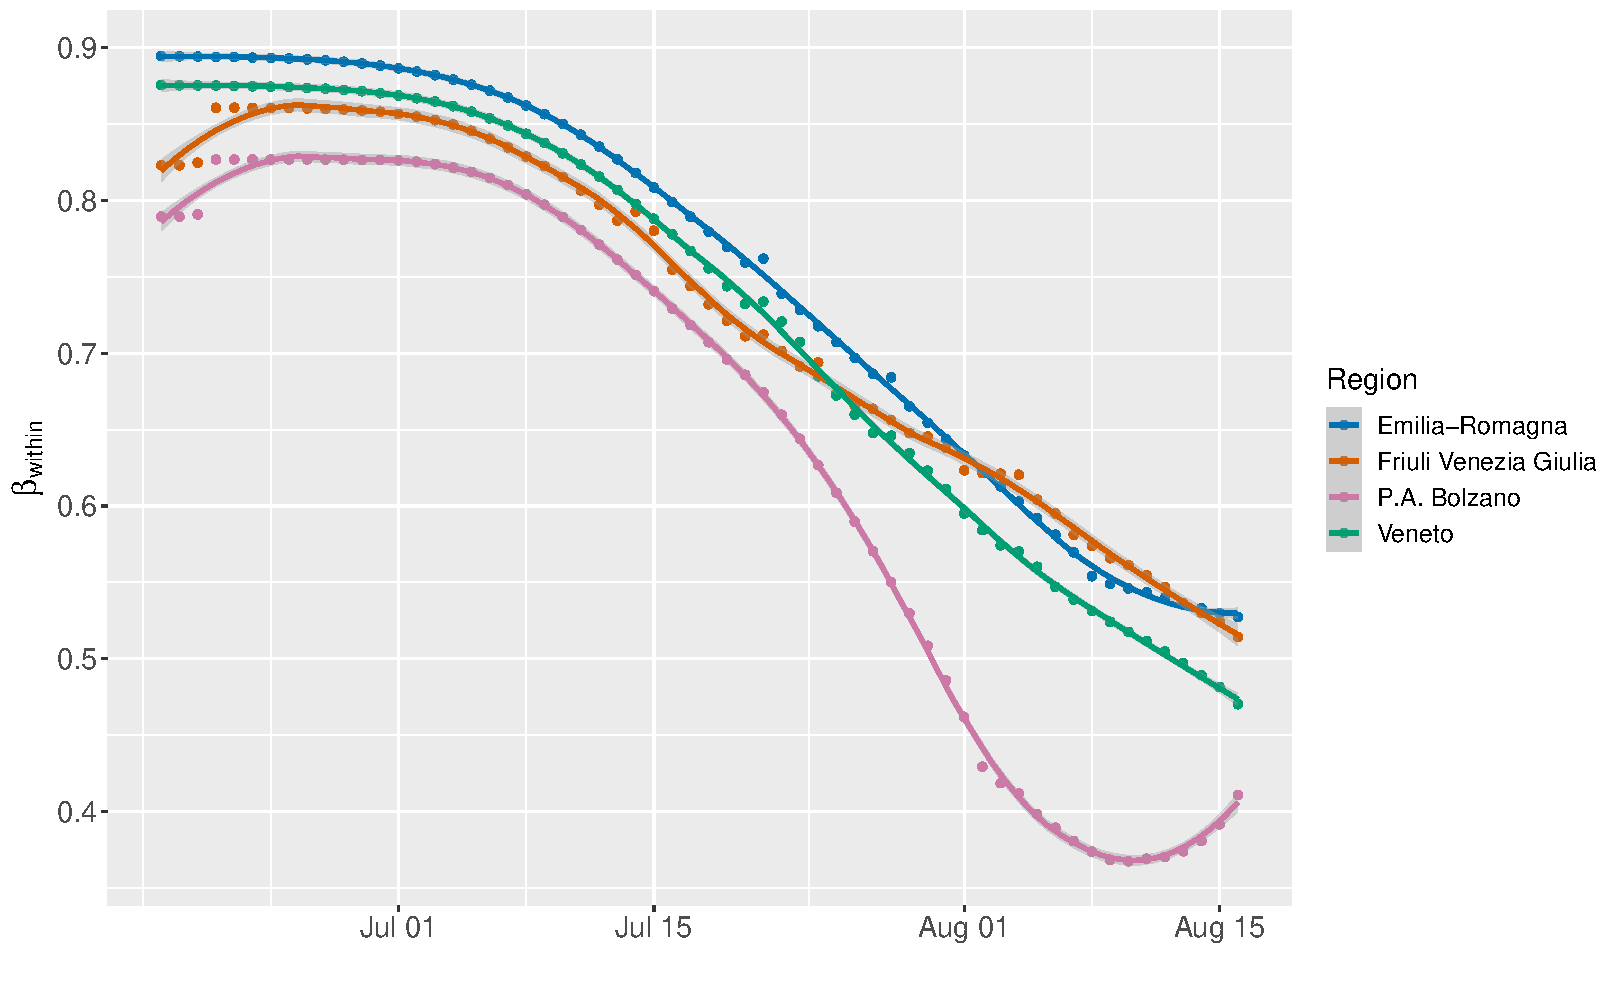
\includegraphics[width=0.92\linewidth]{output/model_within_lag14_betawithin_Nord-Est_aic_UndocQuadratic_rolling.pdf}
	      \caption{With model selection by AIC; \\ including undocumented infectives}
	      \label{fig:beta_within_over_time_nordest_aic_undoc}
	    \end{subfigure}
	    \caption{Progression of $\beta_{within}$ over time for the Nord-Est NUTS 1 region. Data spans May 9 until August 16, 2020 (100 days). Undocumented infectives are modelled using the quadratic specification with $\gamma = 0.7$ and $f^{min}=0.1$.}
	    \label{fig:beta_within_over_time_nordest}
    \end{figure}
	
	Considering the progression of $\beta_{within}$ over time, we indeed see that it decreases over time, as we expected. We do see a slight increase in the estimates of $\beta_{within}$ towards the end of the timespan. This is likely because the amount of infectives increased a bit over time again for multiple regions from mid July onward. Please consider the Figures in Appendix \ref{sapp:figures_problem_description}, which indeed illustrate this increase. We also notice that the pattern of $\beta_{within}$ over time is similar when comparing the models excluding and including undocumented infectives; the difference can be found in the value of $\beta_{within}$ which, as explained earlier in this section, tends to be lower when modelling undocumented infectives.
	
	\section{Within and Between-Region Spread Model} \label{sec:model_between}
	In this section, we present the model by \textcite{adda2016economic} that takes effects across regions into account. Section \ref{subsec:model_between_methodology} discusses the methodology, including the model formulation, estimation method, moment conditions, and the inclusion of undocumented infectives. Subsequently, the results are presented in \ref{subsec:model_between_results}, where we discuss the statistical evidence, the magnitude of the estimates, and how they compare across the regions. Moreover, we investigate the progression of the estimates over time.
	
	\subsection{Methodology} \label{subsec:model_between_methodology}
	In this section, we present the methodology of the within and between-region spread model. A key addition made by \textcite{adda2016economic} is recognizing that there is spatial spillover between regions; there may be infectives in one region that travel to another region and then infect individuals there. The following model is defined:
	\begin{equation} \label{eq:model_between}
	    \Delta i_{p,t} = \beta_{within}S_{p,t-\tau}\Delta i_{p,t-\tau} + \beta_{between}S_{p,t-\tau} \sum_{c \in R \setminus r} \Delta i_{c, t-\tau} + \delta X_{p,t} + \eta_{p,t}.
	\end{equation}
	
	It should be noted that the specification in \eqref{eq:model_between} assumes that individuals from all regions are able to meet one another at the same rate. Of course, this assumption is likely not satisfied. Consider, for example, the region of Lombardy, which lies in north-west Italy. Inhabitants of Lombardy are much more likely to travel to bordering regions, such as Piedmont or Veneto, than to regions in the far south, such as Campania or Apulia, or to the islands. As such, it would be better to consider introducing a method by which we only take a certain number of regions that are the closest to another region into account. Another criterion could be to look at economic ties, since SARS-CoV-2 can not only be transmitted by regular civilians meeting each other but also by the exchange of goods, for example. Spatiotemporal models exist that could be applied when a suitable matrix of weighting measures is available. Nonetheless, in this section, we follow the specification that \textcite{adda2016economic} provides as in \eqref{eq:model_between} and explain the other criteria as possible future research in Section \ref{sec:future_research}. \\
	
	Notice, moreover, that it does not make sense to consider a national model. Because we do not consider countries outside of Italy, the set $R \setminus r$ is empty if we consider $r$ to be the entire country of Italy. This would mean that the national model for the within and between-region spread model is equivalent to the national model for the within-region spread model. As such, in this section, we only consider the model applied to the regions. \\
	
	In \eqref{eq:model_between}, the transmission parameter $\beta$ is now allowed to be different within and between regions. \textcite{adda2016economic} estimates \eqref{eq:model_between} by OLS and by instrumental variable estimation (IV). Weather episodes, such as the amount of rain and temperature-related instruments, are used as instruments. There is a biological reasoning behind choosing these instruments, for instance that warmer temperatures tend to have a negative effect on the proliferation of some viruses. A social reason is also given, namely that bad weather conditions impact the amount of social interaction between people, meaning that there are less opportunities for viruses to spread. We challenge the choice of these instruments, particularly in the case of SARS-CoV-2. Unfortunately, we do not have sufficient information on the effect of the weather on the virus. SARS-CoV-2 has only been quite apparent since January 2020 and there has not been enough fluctuation over time in temperatures to show a necessary effect that can be disentangled from, for example, policies being effective in driving the virus back. Using a spatiotemporal analysis, \textcite{briz2020temperature} even show that no evidence of a relationship between COVID-19 cases and temperature was found, although these results should be interpreted carefully due to data uncertainty and confounders. For these reasons, we only consider OLS for this model. \\
	
	The moment condition that needs to be satisfied due to the strict exogeneity assumption is
	    \[E\left[ \eta_{p,t} \left( \beta_{within} S_{p,t-\tau} \Delta i_{p,t-\tau}  + \beta_{between}S_{p,t-\tau} \sum_{c \in R \setminus r} \Delta i_{c, t-\tau} + \delta X_{p,t} \right) \right] = 0.\]
	    
	\noindent In the same way as in Section \ref{subsec:model_within_methodology}, we can assume that $E\left[\eta_{p,t} \,\middle|\, X_{p,t}\right] = 0$ and \\
	$E\left[\eta_{p,t} \,\middle|\, S_{p,t-\tau} \Delta i_{p,t-\tau}\right] = 0$. Following the same reasoning as before, we assume that the number of infectives who come into contact with susceptible people in other regions at a certain time is not correlated with the error if the lag is large enough, therefore assuming that $E\left[\eta_{p,t} \,\middle|\, \beta_{between}S_{p,t-\tau} \sum_{c \in R \setminus r} \Delta i_{c, t-\tau}\right] = 0$. As such, we assume that the moment condition holds. \\
	
	Using the specification of undocumented infectives, we can adapt the within and between-region spread model to include these undocumented infectives as well. Using that $\Delta i_{p,t} = \frac{D_{p,t}}{f_{p,t}(\gamma)} - \frac{D_{p,t-1}}{f_{p,t-1}(\gamma)}$, the model in \eqref{eq:model_between} becomes:
	
	    \begin{equation} \label{eq:model_between_undocumented}
            \begin{split}
        		\frac{D_{p,t}}{f_{p,t}(\gamma)} - \frac{D_{p,t-1}}{f_{p,t-1}(\gamma)} = &\beta_{within}S_{p,t-\tau}\left(\frac{D_{p,t-\tau}}{f_{p,t-\tau}(\gamma)} - \frac{D_{p,t-\tau-1}}{f_{p,t-\tau-1}(\gamma)}\right) \\
    		    &+ \beta_{between}S_{p,t-\tau} \sum_{c \in R \setminus r} \left(\frac{D_{c,t-\tau}}{f_{c,t-\tau}(\gamma)} - \frac{D_{c,t-\tau-1}}{f_{c,t-\tau-1}(\gamma)} \right) \\
    		    &+ \delta X_{p,t} + \eta_{p,t}.
    		\end{split}
        \end{equation}
	
	\noindent We can rewrite \eqref{eq:model_between_undocumented} as follows
	    \begin{align*}
	       D_{p,t} = f_{p,t}(\gamma)\Bigg(&\beta_{within}S_{p,t-\tau}\left(\frac{D_{p,t-\tau}}{f_{p,t-\tau}(\gamma)} - \frac{D_{p,t-\tau-1}}{f_{p,t-\tau-1}(\gamma)}\right) \\
	       &+ \beta_{between}S_{p,t-\tau} \sum_{c \in R \setminus r} \left(\frac{D_{c,t-\tau}}{f_{c,t-\tau}(\gamma)} - \frac{D_{c,t-\tau-1}}{f_{c,t-\tau-1}(\gamma)} \right) \\
	       & + \frac{D_{p,t-1}}{f_{p,t-1}(\gamma)} + \delta X_{p,t} + \eta_{p,t}\Bigg).
	    \end{align*}
	    
	\noindent The moment conditions that then need to hold are:
	    \begin{equation} \label{eq:model_between_undocumented_moments}
            \begin{split}
    	        E\Bigg[ f_{p,t}(\gamma) \eta_{p,t}\Bigg( &\beta_{within}S_{p,t-\tau}\left(\frac{D_{p,t-\tau}}{f_{p,t-\tau}(\gamma)} - \frac{D_{p,t-\tau-1}}{f_{p,t-\tau-1}(\gamma)}\right) \\
    	        &+ \beta_{between}S_{p,t-\tau} \sum_{c \in R \setminus r} \left(\frac{D_{c,t-\tau}}{f_{c,t-\tau}(\gamma)} - \frac{D_{c,t-\tau-1}}{f_{c,t-\tau-1}(\gamma)} \right) \\
    	        &+ \frac{D_{p,t-1}}{f_{p,t-1}(\gamma)} + \delta X_{p,t} \Bigg) \Bigg] = 0.
	        \end{split}
        \end{equation}
	
	Since $f_{p,t}(\gamma)$ is simply a scaling function, regardless of the chosen parameter, it has no influence on the dependence between the error and the regressors. As such, it can be taken out of the expectation term. Subsequently, we can divide both sides of the equation by $f_{p,t}(\gamma)$ to obtain the following moment condition:
        \begin{align*}
    		E\Bigg[ \eta_{p,t}\Bigg( &\beta_{within}S_{p,t-\tau}\left(\frac{D_{p,t-\tau}}{f_{p,t-\tau}(\gamma)} - \frac{D_{p,t-\tau-1}}{f_{p,t-\tau-1}(\gamma)}\right) \\
	        &+ \beta_{between}S_{p,t-\tau} \sum_{c \in R \setminus r} \left(\frac{D_{c,t-\tau}}{f_{c,t-\tau}(\gamma)} - \frac{D_{c,t-\tau-1}}{f_{c,t-\tau-1}(\gamma)} \right) \\
	        &+ \frac{D_{p,t-1}}{f_{p,t-1}(\gamma)} + \delta X_{p,t} \Bigg) \Bigg] = 0.
        \end{align*}
	
	Just like before, we make the assumption that the idiosyncratic error $\eta_{p,t}$ is uncorrelated with the regressors in the tensor $X_{p,t}$. Therefore, we assume that $E\left[\eta_{p,t} \,\middle|\, X_{p,t}\right] = 0$. Now note that there are three additional terms to consider, namely the relation between $\eta_{p,t}$ and $S_{p,t-\tau}\left(\frac{D_{p,t-\tau}}{f_{p,t-\tau}(\gamma)} - \frac{D_{p,t-\tau-1}}{f_{p,t-\tau-1}(\gamma)}\right)$, $S_{p,t-\tau} \sum_{c \in R \setminus r} \left(\frac{D_{c,t-\tau}}{f_{c,t-\tau}(\gamma)} - \frac{D_{c,t-\tau-1}}{f_{c,t-\tau-1}(\gamma)} \right)$, and $\frac{D_{p,t-1}}{f_{p,t-1}(\gamma)}$, the first and last of which have been discussed in Section \ref{subsec:model_between_methodology}. That leaves the middle term, for which the reasoning is identical to the first term: for a large enough lag $\tau$, the error is not correlated with past data at that lag, which is independent of the scaling functions $f_{p,t-\tau}(\gamma)$ and $f_{p,t-\tau-1}(\gamma)$ as these are constructed without the past infectives in mind. We also say that it does not matter whether we consider infectives within the region or in other regions, as the longer time lag applies in any case. Therefore, we assume that the moment conditions in \eqref{eq:model_between_undocumented_moments} hold, even when modelling undocumented infectives.
	
	\subsection{Results} \label{subsec:model_between_results}
	In this section, we present the results for the within and between-region spread model. If no statistical significance level is mentioned, we take a significance level of 0.05. Once again, we use the last 100 days of data, which spans May 9 until August 16. \\
	
	In Table \ref{tab:results_between_aic}, we present the results where we execute model selection using the AIC and we make sure that the terms for $\beta_{within}$ and $\beta_{between}$ remain in the model, meaning that model selection is solely performed on whether the weekend dummy should be included. In Table \ref{tab:results_between_no_ms} in Appendix \ref{app:tables}, we present the results without applying model selection. The results comparing the use of the BIC over the AIC for model selection are presented in Table \ref{tab:results_between_aic_vs_bic}.
	
	\begin{longtable}{@{}lcccccc@{}}
		\caption{Estimates from the within and between-region spread model per region with model selection by AIC. Estimates are given with $t$-statistics in parentheses. Data spans May 9 until August 16, 2020 (100 days). Undocumented infectives are modelled using the quadratic specification with $\gamma = 0.7$ and $f^{min}=0.1$.}
		\label{tab:results_between_aic}\\
		\toprule
		                & \multicolumn{3}{c}{Regular model} & \multicolumn{3}{c}{Modelling undocumented infectives} \\
		                \cmidrule(lr){2-4}
                        \cmidrule(lr){5-7}
		Region          & $\beta_{within}$ & $\beta_{between}$ & Weekend & $\beta_{within}$ & $\beta_{between}$ & Weekend \\* \midrule
		\endfirsthead
		
		\multicolumn{7}{c}{{\bfseries Table \thetable\ continued from previous page}} \\
		\toprule
		                & \multicolumn{3}{c}{Regular model} & \multicolumn{3}{c}{Modelling undocumented infectives} \\
		                \cmidrule(lr){2-4}
                        \cmidrule(lr){5-7}
		Region          & $\beta_{within}$ & $\beta_{between}$ & Weekend & $\beta_{within}$ & $\beta_{between}$ & Weekend \\* \midrule
		\endhead
		
		\bottomrule
		\multicolumn{7}{c}{{\bfseries Table \thetable\ continues on next page}}
		\endfoot
		
		\multicolumn{7}{c}{Significance levels: * = 0.1 ** = 0.05, *** = 0.01}
		\endlastfoot
		
        Abruzzo & $-0.011$ & $5.871 \times 10^{-3}$*** & 2.394* & $-0.047$ & $5.943 \times 10^{-3}$*** & 12.494** \\
         & ($-0.079$) & (3.399) & (1.909) & ($-0.495$) & (4.455) & (2.279) \\ 
        Basilicata & 0.040 & $7.638 \times 10^{-4}$ &  & 0.034 & $6.299 \times 10^{-3}$ &  \\ 
         & (0.357) & (1.286) &  & (0.321) & (1.379) &  \\ 
        P.A. Bolzano & 0.246** & $2.043 \times 10^{-4}$ & 2.305*** & 0.201** & $1.018 \times 10^{-4}$ & 7.030*** \\ 
         & (2.355) & (0.317) & (3.534) & (2.559) & (0.310) & (3.848) \\ 
        Calabria & 0.186 & $7.936 \times 10^{-4}$ & 1.893** & 0.128 & $8.270 \times 10^{-4}$ & 11.514** \\ 
         & (1.460) & (1.171) & (2.168) & (1.088) & (1.341) & (2.472) \\ 
        Emilia-Romagna & 0.365*** & $-8.645 \times 10^{-4}$ & 22.410*** & 0.171*** & 0.015* & 90.384*** \\ 
         & (4.184) & ($-0.080$) & (4.817) & (2.635) & (1.873) & (5.267) \\ 
        Friuli Venezia Giulia & 0.114* & $3.701 \times 10^{-3}$*** & 1.759** & 0.034 & $3.026 \times 10^{-3}$*** & 4.330** \\ 
         & (1.707) & (4.346) & (2.481) & (0.929) & (7.601) & (2.139) \\ 
        Lazio &  0.342*** & $7.364 \times 10^{-3}$ & 10.573*** & 0.238** & 0.010* & 61.107*** \\
         & (2.671) & (1.283) & (3.568) & (2.221) & (1.853) & (3.879) \\ 
        Liguria & $-0.026$ & 0.033*** &  & $-0.023$ & 0.029*** &  \\ 
         & ($-0.372$) & (6.515) &  & ($-0.404$) & (6.613) &  \\ 
        Lombardy & 0.329*** & 0.226*** &  & 0.285*** & 0.190*** &  \\ 
         & (4.929) & (4.257) &  & (4.463) & (3.926) &  \\ 
        Marche & 0.245** & $4.505 \times 10^{-3}$** & 2.150* & 0.181** & $4.644 \times 10^{-3}$*** & 10.483* \\ 
         & (2.521) & (2.229) & (1.710) & (2.312) & (2.907) & (1.921) \\ 
        Molise & $-0.085$ & $4.063 \times 10^{-3}$*** &  & $-0.077$ & $4.596 \times 10^{-3}$*** &  \\ 
         & ($-1.168$) & (8.821) &  & ($-1.158$) & (9.811) &  \\ 
        Piedmont & 0.104*** & 0.065*** &  & 0.091*** & 0.057*** &  \\ 
         & (3.665) & (9.767) &  & (3.882) & (9.785) &  \\ 
        Apulia & 0.120 & $5.525 \times 10^{-3}$*** & 3.083** & 0.035 & $8.078 \times 10^{-3}$*** & 18.908** \\ 
         & (1.051) & (2.629) & (2.115) & (0.393) & (3.896) & (2.303) \\ 
        Sardinia & 0.407*** & $1.846 \times 10^{-3}$ &  & 0.252** & $1.831 \times 10^{-4}$ & 5.062 \\ 
         & (2.903) & (0.299) &  & (2.468) & (0.321) & (1.532) \\ 
        Tuscany & 0.051 & 0.010*** & 8.023*** & 0.030 & $9.454 \times 10^{-3}$*** & 33.901*** \\ 
         & (0.605) & (3.107) & (3.812) & (0.535) & (4.141) & (4.095) \\ 
        Umbria & 0.427*** & $4.689 \times 10^{-5}$ & 1.410*** & 0.235** & $2.449 \times 10^{-4}$ & 4.877*** \\ 
         & (2.981) & (0.102) & (2.904) & (2.467) & (0.876) & (2.832) \\ 
        Aosta Valley & 0.023 & $1.111 \times 10^{-3}$*** &  & 0.055 & $7.104 \times 10^{-4}$*** &  \\ 
         & (0.259) & (4.193) &  & (0.775) & (4.374) &  \\ 
        Veneto & 0.904*** & $-0.033$*** & 16.184*** & 0.434*** & $-7.954 \times 10^{-3}$ & 43.868*** \\
         & (6.990) & ($-3.771$) & (2.721) & (4.370) & ($-1.637$) & (2.951) \\* \bottomrule
	\end{longtable}
	
	We first discuss the statistical evidence for the estimated values of $\beta_{within}$ and $\beta_{between}$ and how these interact. After this, we consider the interpretation of the coefficients and the model selection. Before that, there are two things to notice to start with. Firstly, notice that the estimates for $\beta_{between}$ are generally much smaller than the estimates for $\beta_{within}$. This is likely the case because \textcite{adda2016economic} defined the models with the absolute number of new cases instead of a proportion. As such, summing over all regions leads to a large number of total new cases, causing the parameter estimate to be driven down. A notable exception being the region of Lombardy, where the estimate for $\beta_{between}$, namely 0.378, is indeed smaller than the estimate for $\beta_{within}$, namely 0.514, but the two estimates are much closer than for other regions. A similar result can be found for the region of Piedmont. For the region of Lombardy, the reason for the estimates being much closer is twofold. Firstly, because it is the largest region in Italy, housing around one-sixth (16.67\%) of the total population of Italy, where the second-largest region is Lazio, which houses 9.74\% of the total amount of Italians. Secondly, Lombardy was hit the hardest by SARS-CoV-2 of all of the Italian regions and, therefore, the number of infectives there is much higher than in other regions. As such, summing the other regions has a proportionally smaller effect. \\
	
	The second matter to be noticed is that there are negative values of the estimates of $\beta_{within}$ and $\beta_{between}$, which happens three and two out of eighteen times, respectively, for the regular model. For the model including undocumented infectives, this happens three times (for the same three regions) and once (the estimate for Emilia-Romagna is now positive), respectively. This should not be possible because this means that when infectives meet susceptible people, the incidence rate decreases. Luckily, these estimates are generally not statistically significant, with an exception for the estimate of $\beta_{between}$ for Veneto in the regular model, for which the estimate is significant at a significance level of 0.01. Future research can be done into models that restrict the estimates to be positive. \\
	
	On the topic of statistical significance, recall that there was only one region that did not have a statistically significant estimate for $\beta_{within}$ for the within-region spread model at a significance level of 0.05, namely Basilicata. For the within and between-region spread model, we also find no statistically significant results for Basilicata, neither for $\beta_{within}$ and $\beta_{between}$. This also happens for the region of Calabria. In addition, nine and eleven out of eighteen regions find a significant estimate for $\beta_{within}$ and $\beta_{between}$, respectively, when excluding undocumented infectives. For the model including undocumented infectives, ten regions find a significant result for $\beta_{between}$, the difference being that the (negative) result for Veneto is no longer significant. The same nine regions as for the regular model once again find a significant result for $\beta_{within}$. \\
	
	However, if a significant result for $\beta_{between}$ is found, this does not necessarily go hand-in-hand with a significant estimate for $\beta_{within}$ or vice versa. For the regular model, it only happens four times that the estimates are jointly significant, namely for Lombardy, Marche, Piedmont, and Veneto. For the model including undocumented infectives, this happens only three times, namely for the same regions excluding Veneto. \\
	
	Looking only at the statistically significant estimates of $\beta_{within}$, these range from 0.104 for Piedmont until 0.904 for Veneto for the regular model and from 0.091 for Piedmont until 0.434 for Veneto when undocumented infectives are included. Excluding Veneto, the highest values for the regular model and the model including undocumented infectives are 0.427 for Umbria and 0.285 for Lombardy, respectively. Therefore, we notice that the estimates for Veneto are outliers and that the values are a bit lower than for the within-region model. When considering the statistically significant estimates of $\beta_{between}$, we see that these range from $1.111 \times 10^{-3}$ for Aosta Valley until 0.226 for Lombardy for the regular model and from $7.104 \times 10^{-4}$ for Aosta Valley until 0.190 for Lombardy when undocumented infectives are included. Conclusively, we see that the estimates of $\beta_{between}$ differ much less over the regions than those of $\beta_{within}$. \\
	
	One aspect to pay attention to is regarding the impact of modelling undocumented infectives on the estimates. Notice that modelling undocumented infectives again causes the (significant) estimates of $\beta_{within}$ to be lower than for the regular model, just like for the within-region spread model. For $\beta_{between}$, however, this is not the case. For four out of ten cases, namely for Abruzzo, Marche, Molise, and Apulia, where both estimates of $\beta_{between}$ are significant, the estimate when modelling undocumented infectives is higher. We believe that this is likely the case because all regions are affected in a similar way by the modelling method of undocumented infectives, although the regions that test more rigorously are of course affected less. As such, there is no uniform way in which the estimate is affected. Also consider Figure \ref{fig:tamponiprop_versus_ft}, where we plotted the testing capacity versus the proportion of undocumented infectives for our modelling method. We do not see that a certain pattern happens for the four aforementioned regions that does not happen for other regions that find significant estimates of $\beta_{between}$, such as Lombardy, Piedmont, and Tuscany. \\
	
	To investigate whether the differences in the estimates differ significantly, we consider the regions of Lombardy, Marche, and Piedmont since these are the only regions that find statistically significant results for all four estimates. For $\beta_{within}$, we find $t$-statistics of 0.476, 0.513, and 0.353, respectively. None of these exceed the critical value of $t_{T;0.95} = 1.96$, meaning that modelling undocumented infectives does not cause a significant difference in these estimates. There is one exception. For Veneto, the $t$-statistic of 2.882 does exceed the critical value. For $\beta_{between}$, we find $t$-statistics of 0.501, $-0.054$, and 0.905, respectively. Once again, no statistical difference can be found. One can check that none of the estimates for $\beta_{between}$, when both are significant, differ significantly. \\
	
	Recall that we cannot interpret the coefficients in the same way as \textcite{adda2016economic} does but that we can compare the magnitude of the coefficients with one another across regions. For instance, let us compare the regions of Lombardy and Piedmont. For both regions, all estimates are statistically significant. We consider the model including undocumented infectives. We find estimates of $\beta_{within}$ of 0.285 and 0.091 and estimates of $\beta_{between}$ of 0.190 and 0.057 for Lombardy and Piedmont, respectively. We can conclude that the transmission within the region as well as between regions was worse in Lombardy compared to Piedmont, although we cannot explicitly interpret the magnitude of that transmission. \\
	
    Regarding model selection, the set of regressors that is used is the same whether undocumented infectives are modelled are not, except for the island of Sardinia. All models retain the terms related to $\beta_{within}$ and $\beta_{between}$ in the model. For Sardinia, the weekend dummy is excluded in the regular model but it is included when undocumented infectives are modelled. In eleven out of the remaining seventeen cases, the entire model is selected. In the other six cases, the weekend dummy is excluded. \\
    
    To conclude, we are again interested in looking at the estimates of $\beta_{within}$ and $\beta_{between}$ over time. In Figure \ref{fig:beta_between_over_time_nordest}, we present plots for the regions in the Nord-Est NUTS 1 region. Plots for the other NUTS 1 regions can be found in Appendix \ref{sapp:model_between_figures}. Each point in the graphs in Figure \ref{fig:beta_between_over_time_nordest} is the estimate of $\beta_{within}$ or $\beta_{between}$ when only the latest 100 data points before that date are used. In addition, a LOESS curve with span parameter 0.3 is fit to the data points.
    
    \begin{figure}[H]
	    \centering
	    \begin{subfigure}{\textwidth}
	      \centering
	      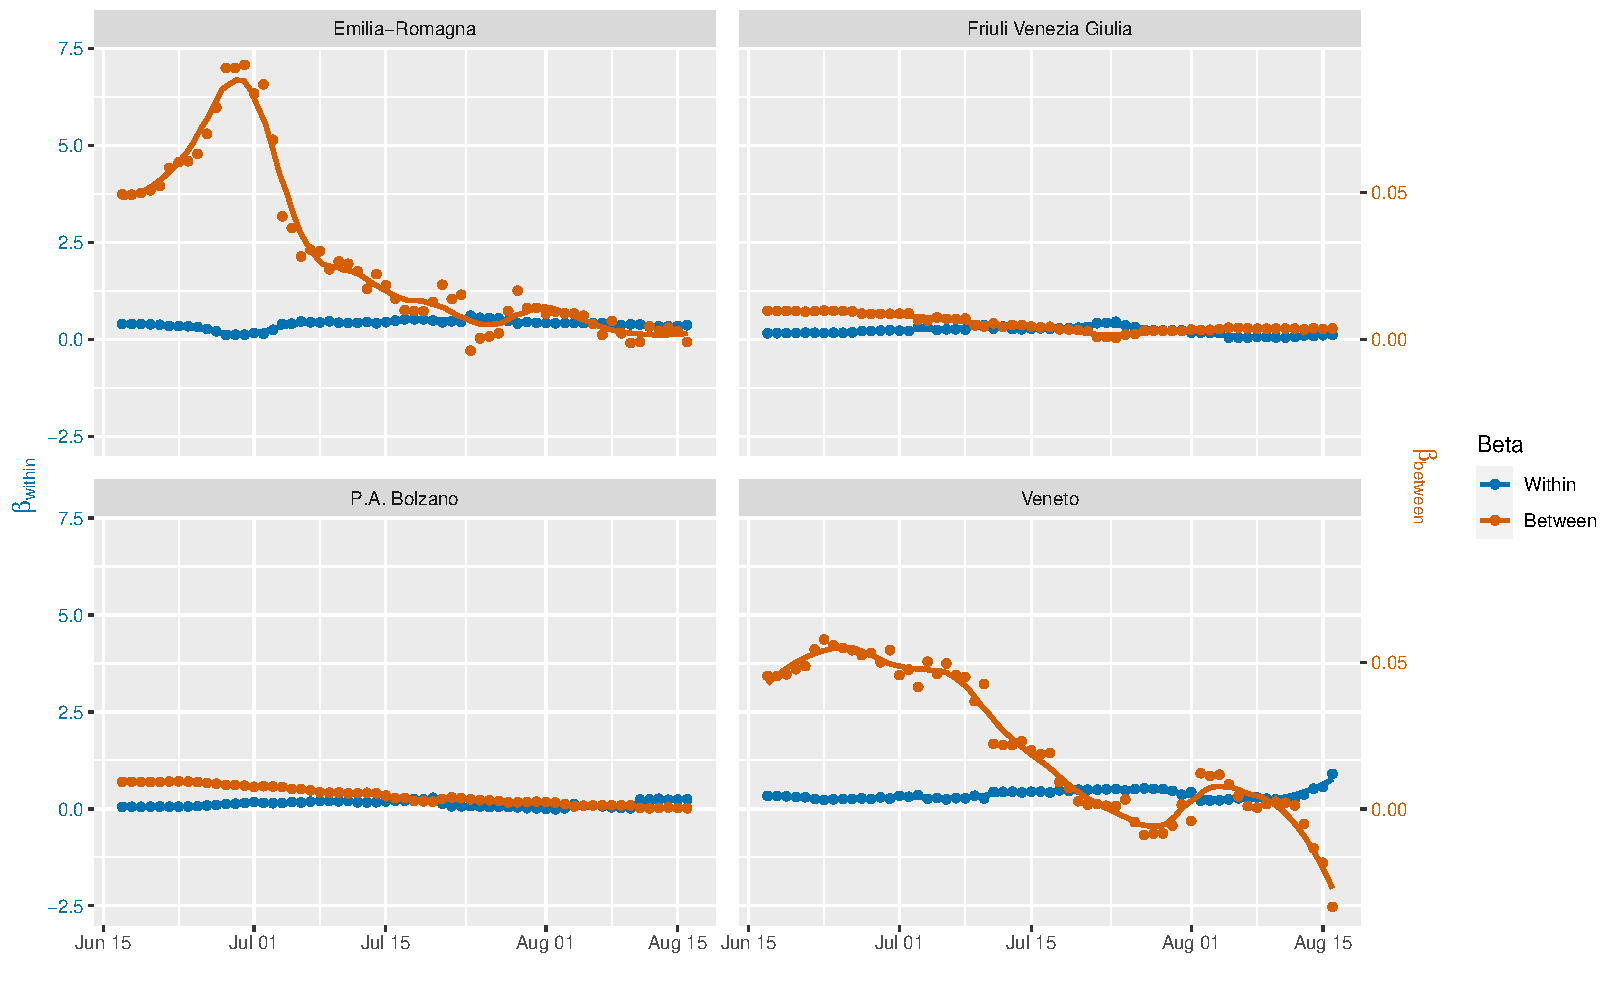
\includegraphics[width=\linewidth]{output/model_between_lag14_betas_Nord-Est_rolling.pdf}
	      \caption{Without model selection}
	      \label{fig:beta_between_over_time_nordest_regular}
	    \end{subfigure}
    \end{figure}
    \begin{figure}[H]\ContinuedFloat
	    \begin{subfigure}{\textwidth}
	      \centering
	      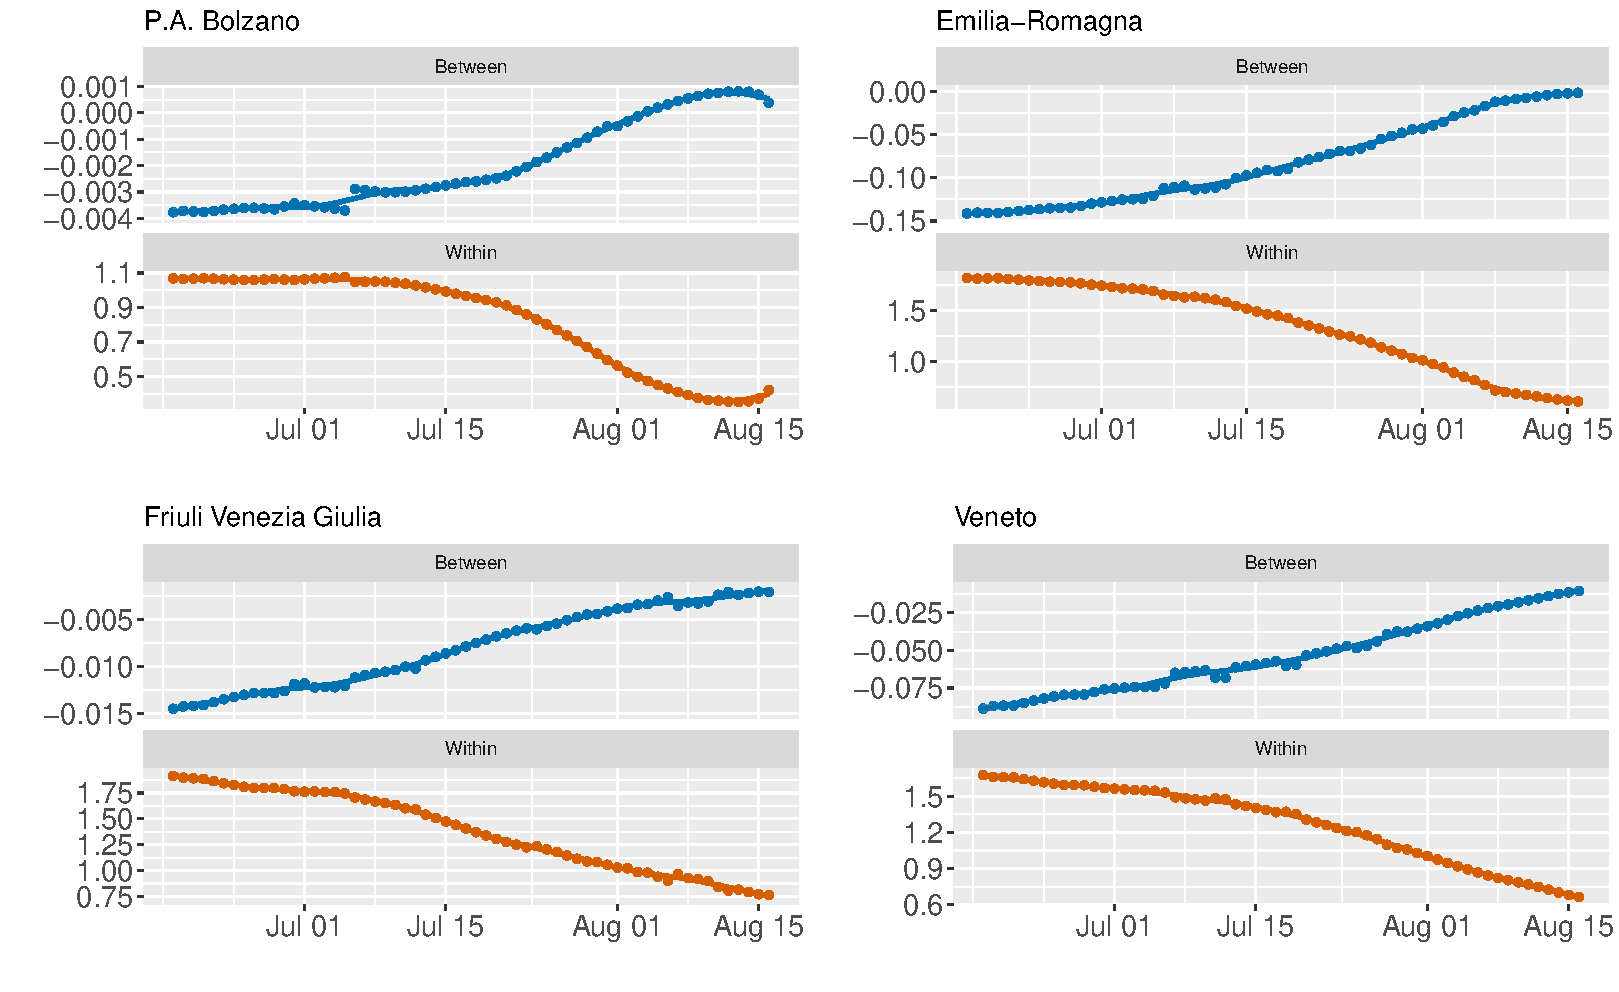
\includegraphics[width=\linewidth]{output/model_between_lag14_betas_Nord-Est_aic_rolling.pdf}
	      \caption{With model selection by AIC}
	      \label{fig:beta_between_over_time_nordest_aic}
	    \end{subfigure}
	\end{figure}
    \begin{figure}[H]\ContinuedFloat
	    \begin{subfigure}{\textwidth}
	      \centering
	      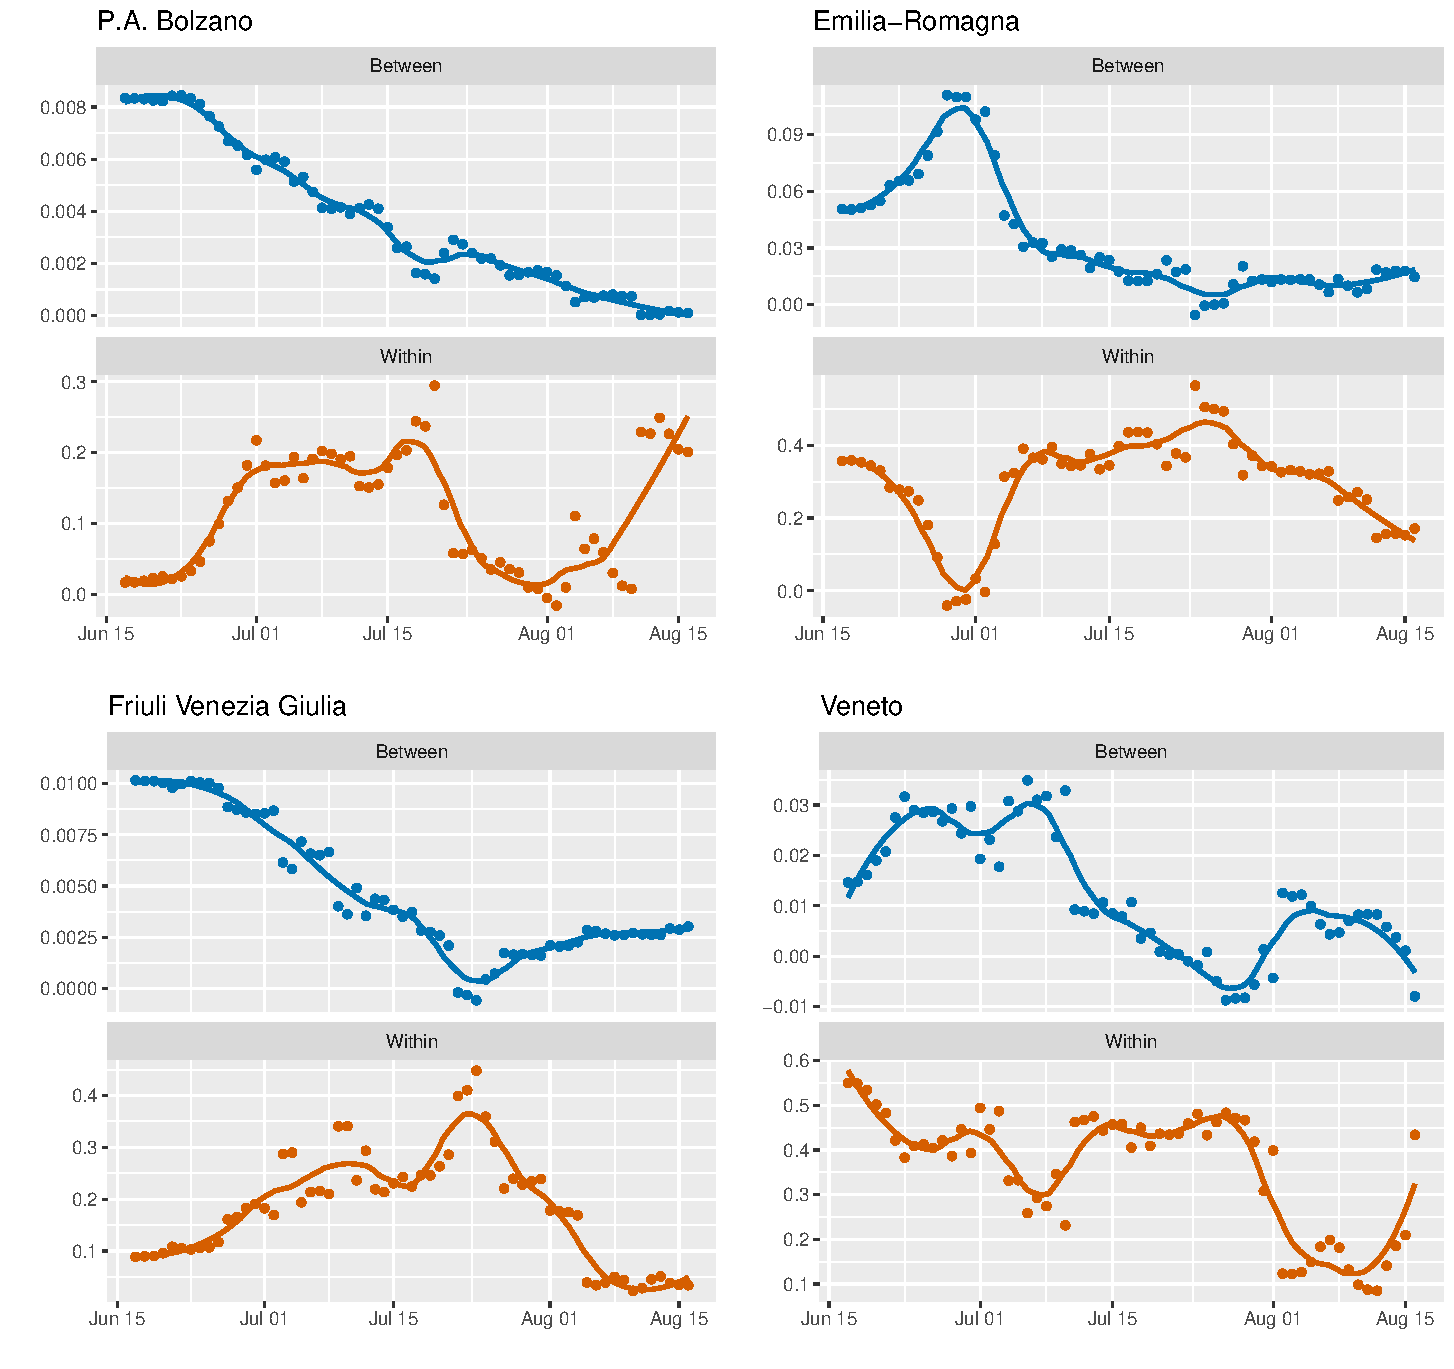
\includegraphics[width=\linewidth]{output/model_between_lag14_betas_Nord-Est_UndocQuadratic_rolling.pdf}
	      \caption{Without model selection; \\ including undocumented infectives}
	      \label{fig:beta_between_over_time_nordest_regular_undoc}
	    \end{subfigure}
    \end{figure}
    \begin{figure}[H]\ContinuedFloat
	    \begin{subfigure}{\textwidth}
	      \centering
	      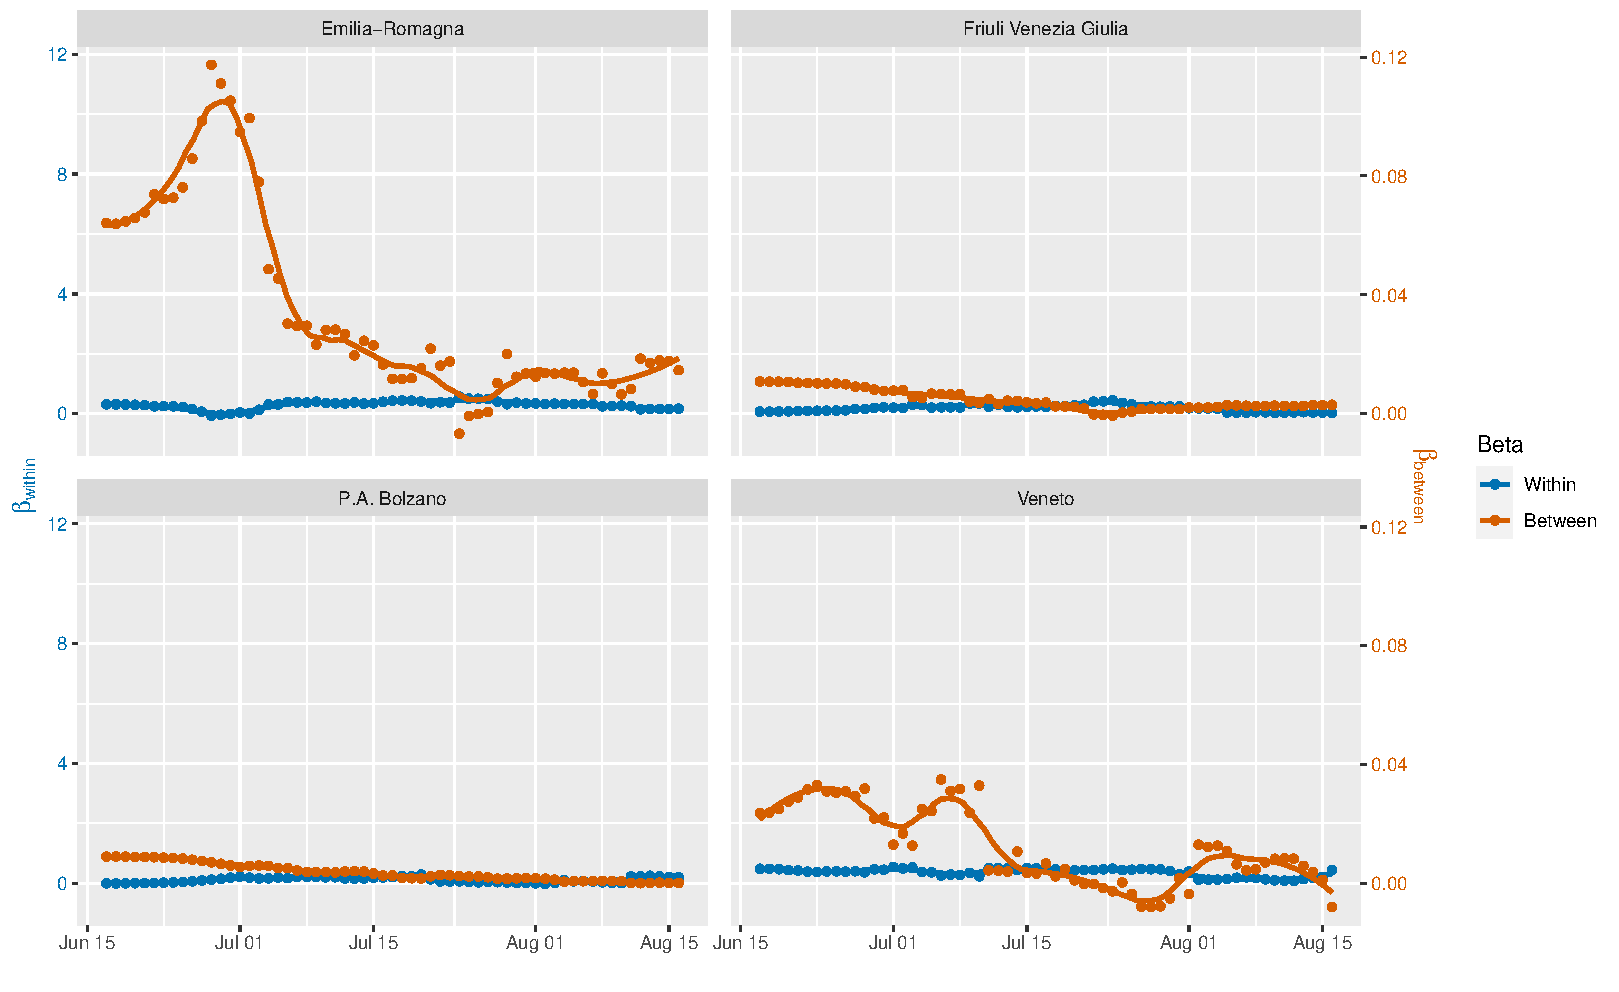
\includegraphics[width=\linewidth]{output/model_between_lag14_betas_Nord-Est_aic_UndocQuadratic_rolling.pdf}
	      \caption{With model selection by AIC; \\ including undocumented infectives}
	      \label{fig:beta_between_over_time_nordest_aic_undoc}
	    \end{subfigure}
	    \caption{Progression of $\beta_{within}$ and $\beta_{between}$ over time for the Nord-Est NUTS 1 region. Data spans May 9 until August 16, 2020 (100 days). Undocumented infectives are modelled using the quadratic specification with $\gamma = 0.7$ and $f^{min}=0.1$.}
	    \label{fig:beta_between_over_time_nordest}
    \end{figure}
	
	Figure \ref{fig:beta_between_over_time_nordest} shows very different patterns compared to the within-region spread model, as discussed in the previous section. Generally, we do not see a decreasing movement for $\beta_{within}$. In contrast, the values seem to fluctuate. For $\beta_{between}$, we also see some fluctuation but we do see a decreasing movement. For some regions, we even see that $\beta_{within}$ and $\beta_{between}$ seem to move in opposite directions. For example, consider Figure \ref{fig:beta_between_over_time_nordest_aic_undoc} where model selection is applied and undocumented infectives are included. For Emilia-Romagna and Veneto, this observation is immediately visible. For Friuli Venezia Giulia, it also seems to hold, although it is less pronounced. The transmission rates for Bolzano seem to not adhere to this observation. For the other NUTS 1 regions, we see some similar patterns although the progression varies a lot over the regions. For instance, the estimate for $\beta_{between}$ for the region of Lazio tends to increase over time, as can be seen in Figure \ref{fig:beta_between_over_time_centro}. \\
	
	Conclusively, it seems like neither model selection by AIC and modelling undocumented infectives have a large impact on the profiles of the estimates of $\beta_{within}$ and $\beta_{between}$ much, besides the impact on the magnitude of the values, as explained in the discussion of Table \ref{tab:results_between_aic}.
	
% 	\section{Discrete SIR Model}\label{sec:discrete_sir_model}
% 	As explained in Section \ref{subsec:model_within_methodology}, there are several steps made by \textcite{adda2016economic} that are not explained clearly in the paper and that do not seem to mathematically grounded. In this section, we provide our own derivation for a discrete SIR model. We start by explaining the two versions of the SIR model, as eluded to in Section \ref{sec:sir_model}, after which we will describe our own discrete SIR model. Lastly, we will discuss the two methods that are being used to estimate the parameters, in addition to the regional split, in Sections \ref{subsec:discrete_sir_panel} and \ref{subsec:discrete_sir_bayesian}. \\
	
% 	As mentioned in Section \ref{sec:sir_model}, there are two versions of the SIR model, namely with frequency-dependent and with density-dependent transmission. For the former, the proportion of people in each of the groups is used ($S$, $I$, and $R$) while in the latter, the absolute number of people is used ($s$, $i$, and $r$). \textcite{keeling2011modeling} explain that the distinction in applicability is based on the assumption that we make on the relationship between the contact rate and the population size. For frequency-dependent transmission, also called random mixing, these are assumed to be independent whereas for density-dependent transmission it is assumed that the contact rate increases with the population density. Therefore, \textcite{keeling2011modeling} state that frequency-dependent transmission is generally applied when considering a heterogeneous contact structure, which means that everyone interacts with one another with equal probability. Density-dependent transmission is, on the other hand, generally applied to plant and animal diseases. \\
	
% 	To illustrate the logic behind this, consider an infection that is transmitted sexually. \textcite{keeling2011modeling} give an example for chlamydia in a koala population. When considering a human population, frequency-dependent transmission is often used because a higher density of people does not seem to imply a higher sexual activity, i.e. the sexual contact structure is heterogenous. For some animals, however, a higher density may imply that more sexual activity occurs and, therefore, density-dependent transmission may be more applicable. \\
	
% 	Now, let us consider the coronavirus SARS-CoV-2. Firstly, notice that we consider a human population so, therefore, frequency-dependent transmission may be more applicable. However, it is also intuitive that the transmission of SARS-CoV-2 is higher at the moment that more people live in a certain area because, at that point, people can be expected to come into contact with one another more. However, policies that are employed by governments may guarantee a less density-dependent situation, for instance, when governments instate a lockdown, oblige the use of face masks, or promote social distancing. Around 70\% of the papers assume no relationship between density and transmission. In the other 30\% of the cases, a linear relationship is assumed \parencite{nightingale2020importance}. The issue with this, according to \textcite{nightingale2020importance}, is that, respectively, there is an underestimation or overestimation of the delay in infection resurgence after mass quarantining ends. Because we are not interested in estimating the infection resurgence, we expect these issues to not be apparent, although we recognize that a transmission structure that lies somewhere in between would be ideal. \\
	
% 	In this thesis, we look at both versions of the SIR model and compare the results in Section \ref{subsec:discrete_sir_results}. The derivations that are done in this section are for the frequency-dependent version of the SIR model. Of course, we can simply replace the variables $S$, $I$, and $R$ by $s$, $i$, and $r$, respectively, to obtain the formulations for the models using density-dependent transmission. \\
	
% 	Recall from \eqref{eq:SIR_model_S}-\eqref{eq:SIR_model_R} that the SIR model with frequency-dependent transmission is given by:
% 	    \begin{align*}
%     	    \frac{dS}{dt} &= -\beta SI + \omega R, \\
%     	    \frac{dI}{dt} &= \beta SI - \gamma I, \\
%     	    \frac{dR}{dt} &= \gamma I - \omega R.
% 	    \end{align*}
	
% 	In Section \ref{sec:sir_model} we discussed that the parameter $\omega$ represents the immunity. We explained that it is currently unclear whether people develop some sort of immunity to COVID-19. However, we did state that this immunity likely lasts long enough throughout our sample since we do not consider an analysis over multiple years. Therefore, under the assumption that $\omega = 0$, these equations simplify to the following:
% 	    \begin{align}
%     	    \frac{dS}{dt} &= -\beta SI, \label{eq:SIR_model_S_simplified} \\
%     	    \frac{dI}{dt} &= \beta SI - \gamma I, \label{eq:SIR_model_I_simplified} \\
%     	    \frac{dR}{dt} &= \gamma I. \label{eq:SIR_model_R_simplified}
% 	    \end{align}
    	
% 	When taking the possible estimation error $\eta_{p,t}$, whether from discretizing or estimating the parameters, into account, these equations are equivalent to:
% 	    \begin{align}
%         	S_{p,t} - S_{p,t-1} &= -\beta S_{p,t-1}I_{p,t-1} + \eta_{p,t}, \label{eq:SIR_model_S_discrete}\\
%         	I_{p,t} - I_{p,t-1} &= \beta S_{p,t-1}I_{p,t-1} - \gamma I_{p,t-1} + \eta_{p,t}, \label{eq:SIR_model_I_discrete}\\
%         	R_{p,t} - R_{p,t-1} &= \gamma I_{p,t-1} + \eta_{p,t}. \label{eq:SIR_model_R_discrete}
%     	\end{align}
	
% 	As such, if the data available on $S$, $I$, and $R$ are indeed deemed to be accurate, then $\beta$ and $\gamma$ are readily estimated from \ref{eq:SIR_model_S_discrete} and \ref{eq:SIR_model_R_discrete}. The results from estimating the parameters in this way are presented in Section \ref{subsec:discrete_sir_results}. \\
	
% 	Because we are interested in the number of infectives, we will consider equation \eqref{eq:SIR_model_I_discrete}. The right-hand side of this equation consists of three terms. Firstly, the term $\beta S_{p,t-1}I_{p,t-1}$ relates to the observation that new infectives are formed due to interaction of infectives with the susceptible population, i.e. the people that move from the group $s$ to the group $i$. In Section \ref{sec:sir_model}, we explained that it is assumed that this rate $\beta$ is constant over time. However, we concede that the addition of introducing a longer lag that \textcite{adda2016economic} makes is valid. Indeed, when a susceptible person meets an infective and consequently gets infected, this person is not immediately infectious themselves. For the same reasons as laid out in Section \ref{subsec:model_within_methodology}, we can replace the lag in the first term by a longer lag $\tau$, which we would set to be equal to the estimated latent period of three days. The following model would then be the result:
% 	    \begin{equation}\label{eq:SIR_model_I_discrete_tau}
%             I_{p,t} - I_{p,t-1} = \beta S_{p,t-\tau}I_{p,t-\tau} - \gamma I_{p,t-1} + \eta_{p,t}
%         \end{equation}
	
% 	Similarly, we transform equation \eqref{eq:SIR_model_S_discrete} in the same way:
% 	    \begin{equation}\label{eq:SIR_model_S_discrete_tau}
%             S_{p,t} - S_{p,t-1} = -\beta S_{p,t-\tau}I_{p,t-\tau} + \eta_{p,t}
%         \end{equation}
	
% 	We will report results with $\tau=1$ and $\tau=3$ in Section \ref{subsec:discrete_sir_results}. The second term in \eqref{eq:SIR_model_I_discrete} is $-\gamma I_{p,t-1}$, which describes the infectives that recover or die from the disease, i.e. the people that move from group $i$ to group $r$. Note that we have not included the lag $\tau$ in this term. This is because when a person recovers from the disease they immediately move to that group. This also applies to the same term in equation \eqref{eq:SIR_model_R_discrete}. Lastly, as mentioned in the previous paragraph, $\eta_{p,t}$ denotes the idiosyncratic error term. \\
	
% 	As mentioned earlier in this section, if one believes the data on all components to be correct, these parameters can be easily identified. However, $S_{p,t-\tau}$ is generally quite close to the value one: most of the population is susceptible to contracting the virus. That means that it is difficult to identify the parameters jointly. Suppose that $S_{p,t-\tau}$ is indeed equal to 1, for simplification purposes. Then, the right-hand side of \eqref{eq:SIR_model_I_discrete_tau} becomes $\beta I_{p,t-\tau} - \gamma I_{p,t-1}$. It is probable that $I_{p,t-\tau}$ and $I_{p,t-1}$ are quite close to one another, meaning that they cannot be jointly identified by means of equation \eqref{eq:SIR_model_I_discrete_tau}. As such, we need to employ a two-step approach. \\
	
% 	We propose two methods. Firstly, we can apply estimation methods to \eqref{eq:SIR_model_S_discrete_tau} and \eqref{eq:SIR_model_R_discrete} individually to obtain the estimates for $\beta$ and $\gamma$ individually. The second method would be to first estimate one of the parameters by means of \eqref{eq:SIR_model_R_discrete} \eqref{eq:SIR_model_S_discrete_tau}. Secondly, we would fill in this estimate in \eqref{eq:SIR_model_I_discrete_tau} and estimate the remaining parameter. We use equation \ref{eq:SIR_model_R_discrete} to estimate $\gamma$ and use the resulting estimate $\hat{\gamma}$ in \eqref{eq:SIR_model_I_discrete_tau} to obtain:
% 	    \begin{align*}
% 	        & I_{p,t} - I_{p,t-1} = \beta S_{p,t-\tau}I_{p,t-\tau} - \hat{\gamma} I_{p,t-1} + \eta_{p,t} \\
% 	        \iff & I_{p,t} - \left(1 - \hat{\gamma}\right) I_{p,t-1} = \beta S_{p,t-\tau}I_{p,t-\tau} + \eta_{p,t} \numberthis{\label{eq:SIR_model_I_discrete_twostep}}
% 	    \end{align*}
	
% 	Another solution, if one does not believe in the accuracy of the data, is to write the difference in the number of removed individuals as a function of the constant rate $\gamma$ and the infectives. This is then included in the calculation of the susceptible population by means of a function, after which nonlinear least-squares (NLS) can be applied. \todo[inline, backgroundcolor=green!40]{TODO: Continue here: NLS}
	
% 	\subsection{Panel data methods}\label{subsec:discrete_sir_panel}
% 	The discrete SIR equations in \eqref{eq:SIR_model_R_discrete}, \eqref{eq:SIR_model_S_discrete_tau}, and \eqref{eq:SIR_model_I_discrete_twostep} are estimated by panel data methods and Bayesian estimation. We first discuss the panel data methods. Panel data refers to a dataset that contains measurements over time for a group of individuals. In our case, the individuals are represented by $P$ regions and we have observations for $T$ time periods. The main motivation behind using panel data methods is that they comprise more information, making them more efficient. Moreover, because the same individual is observed multiple times over time, they are able to identify unobserved individual effects (heterogeneity) that are persistent over time, such as an aversion to spending money or another effect that causes an individual that experienced some event in the past to experience that effect in the future again with a higher probability. A regular cross-sectional model is usually described as:
% 	    \begin{equation}\label{eq:cross-section}
%     	    y_i = x_i'\theta + \epsilon_i, \quad\forall i=1,\dotsc,P
% 	    \end{equation}
% 	where $y$ denotes the dependent variable, $x$ denotes the independent variables, $\theta$ is the vector of parameters to be estimated, and $\epsilon$ is an idiosyncratic error term. \\
	
% 	A panel data model is usually described in a very similar way:
% 	    \begin{equation}\label{eq:paneldata}
% 	        y_{i,t} = x_{i,t}'\theta + \epsilon_{i,t}, \quad\forall i=1,\dotsc,P;~ t=1,\dotsc,T
% 	    \end{equation}
% 	where the error component $\epsilon_{i,t} \coloneqq \alpha_i + u_{i,t}$ is a composite error term, comprising a time-invariant individual effect, denoted by $\alpha_i$, and an idiosyncratic error term, denoted by $u_{i,t} \sim N\left(0, \sigma^2_u\right)$. We assume that the individual effect is not correlated with the regressors:
% 	    \begin{equation}\label{eq:orthogonality_assumption}
% 	        E\left[\alpha_i \,\middle|\, x_{i,1}, \dotsc, x_{i, T}\right] = 0
% 	    \end{equation}
	    
% 	As an example, for equation \eqref{eq:SIR_model_I_discrete_twostep}, note that:
% 	    \begin{equation*}
% 	        y_{i,t} = I_{p,t} - \left(1 - \hat{\gamma}\right) I_{p,t-1}, \quad
% 	        \theta = \beta, \quad
%             x_{i,t} = S_{p,t-\tau}I_{p,t-\tau}, \quad
%             u_{i,t} = \eta_{p,t}
% 	    \end{equation*}
	    
% 	Looking at this notation, we can see that it is safe to impose the assumption that the individual effect and the independent variables are orthogonal: it seems odd to assume that the individual regional effect, which is time-invariant, is correlated with the time-varying incidence rate or susceptible rate of this one specific disease. In the rest of this section, we will follow the notation as in \eqref{eq:paneldata} but one can follow the example to formulate these in terms of the SIR equations. \\
	
% 	There are three main panel data models that are usually applied: the pooled OLS (POLS), fixed effects (FE), and random effects (RE) models. The choice between these models depends on the assumptions that are placed on the individual effect $\alpha_i$. For each of these three methods, we define them and discuss the required exogeneity assumption(s) and possible other interesting features. We will start with the fixed effects model because the way it is defined is inconsistent with the epidemiological literature on the SIR model. Next, we will consider the random effects model, after which we discuss the pooled OLS model. \\
	
% 	The fixed effects model makes no assumptions about the time-invariant individual effect but applies a within-transformation, namely time-demeaning the data, to eliminate it from the model. The effect is that all time-invariant regressors, such as dummy variables gender or one's education level, are also eliminated from the model. The fixed effects model is then to apply OLS to the time-demeaned data to obtain the estimates of $\theta$. The model mentions fixed effects in its name because, in essence, it assumes that each individual (region) has a time-constant intercept. This is assumed to be different from zero; otherwise, we could apply the pooled OLS model described at the end of this section. The SIR model, on the other hand, does not include an intercept in its formulation. The reason behind this is intuitive: there is not some non-zero mean number of new cases that is persistent throughout time for a certain region. Because of this, the fixed effects model is not suitable for our estimation. \\
	
% 	The main idea behind the random effects model is to impose a distribution on the individual effects that can then be included in the error term. The random effects model equation is identical to \eqref{eq:paneldata}, where we assume that $\alpha_i \sim N\left(0, \sigma^2_{\alpha}\right)$. This assumption may indeed be in line with the SIR model because the mean heterogeneous effect is assumed to be zero. Because the individual effect is now included in the error term, we need to impose assumptions on the entire composite error term. Firstly, the random effects model requires the strict exogeneity assumption:
% 	    \begin{equation}\label{eq:strict_exogeneity}
% 	        E\left[u_{i,t} \,\middle|\, \alpha_i, x_{i,1}, \dotsc, x_{i, T}\right] = 0, \quad\forall t=1,\dotsc,T 
% 	    \end{equation}
	    
% 	This assumption essentially says that the variables are not allowed to depend on any of the errors, whether in the past, present, or future. However, because the individual effects are included in the error term, we need strict exogeneity between $\epsilon_{i,t}$ and $x_{i,t}$ as well. This is achieved by the assumption that the individual effect is not correlated with the regressors in \eqref{eq:orthogonality_assumption}. As such, combining the strict exogeneity assumption and the orthogonality assumption, the aforementioned strict exogeneity assumption between $\epsilon_{i,t}$ and $x_{i,t}$ holds. We will not delve into the details of how the random effects model is specifically estimated; suffice to say that it is estimated by generalized least squares (GLS). \\
	
% 	Lastly, we discuss pooled OLS. This model ignores the individual effect, hence treating the data as one large cross-section. This means that the $T$ observations for some individual $i$ are actually treated to be cross-sectional observations of $T$ different individuals. The exogeneity assumption that needs to be satisfied is a simple exogeneity assumption:
% 	    \[E(x_{i,t}\epsilon_{i,t}) = 0 \text{, so } E(x_{i,t}u_{i,t}) = 0 \text{ and } E(x_{i,t}\alpha_i) = 0\]
	
% 	Because we expect that there will be a vast difference between the Italian regions, as eluded to in Section \ref{sec:problem_description}, pooled OLS is likely not a good model for this thesis. Nonetheless, we estimate the results and compare them to those of the random effects model.
	
% 	\subsection{Bayesian estimation methods}\label{subsec:discrete_sir_bayesian}
% 	In the last few months, a lot of research has been done on the spread of SARS-CoV-2 for various locales. Therefore, we may have some idea of what the values of the parameters are likely to be.
% 	\todo[inline, backgroundcolor=green!40]{TODO: Continue here}
	
% 	\subsection{Results}\label{subsec:discrete_sir_results}
% 	\todo[inline, backgroundcolor=green!40]{TODO: Results still need to be inserted}
	
% 	In this section, we present the results for the discrete SIR model presented in Section \ref{sec:discrete_sir_model}. Recall that we mentioned three estimation approaches, namely the regular regional splits as applied for the models by \textcite{adda2016economic}, panel data methods, and Bayesian analysis. We will present the results in said order. For all result tables, we again apply a rolling window as before and report the results for two values of the lag parameter $\tau$, namely 1 and 3, as explained in Section \ref{sec:discrete_sir_model}. \\
	
% 	When applying the methodology as explained in Section \ref{sec:discrete_sir_model} to the regional models, there is no panel data structure anymore. Therefore, the results presented in Tables X\todo[backgroundcolor=green!40]{TODO: Table} are estimated with OLS. First off, we present the results comparing frequency-dependent transmission and density-dependent transmission in Table \ref{tab:results_discrete_regional_transmission}.
	
% 	\begin{landscape}
% 	\begin{longtable}{@{}lccccccc@{}}
% 	    \caption{Estimates for the discrete SIR model per region comparing frequency-dependent and density-dependent transmission. Estimates are given with $t$-statistics in parentheses. Data spans May 9 until August 16, 2020 (100 days). Undocumented infectives are not modelled. A lag of $\tau=1$ is used.}
% 		\label{tab:results_discrete_regional_transmission}\\
% 		\toprule
% 		                & \multicolumn{3}{c}{Frequency-dependence} & \multicolumn{3}{c}{Density-dependence} \\
% 		                \cmidrule(lr){2-4}
%                         \cmidrule(lr){5-7}
% 		Region          & $\beta$ & $\beta_{two-step}$ & $\gamma$ & $\beta$ & $\beta_{two-step}$ & $\gamma$ \\* \midrule
% 		\endfirsthead
		
% 		\multicolumn{7}{c}{{\bfseries Table \thetable\ continued from previous page}} \\
% 		\toprule
% 		                & \multicolumn{3}{c}{Frequency-dependence} & \multicolumn{3}{c}{Density-dependence} \\
% 		                \cmidrule(lr){2-4}
%                         \cmidrule(lr){5-7}
% 		Region          & $\beta$ & $\beta_{two-step}$ & $\gamma$ & $\beta$ & $\beta_{two-step}$ & $\gamma$ \\* \midrule
% 		\endhead
		
% 		\bottomrule
% 		\multicolumn{7}{c}{{\bfseries Table \thetable\ continues on next page}}
% 		\endfoot
		
% 		\multicolumn{7}{c}{Significance levels: * = 0.1 ** = 0.05, *** = 0.01}
% 		\endlastfoot
%         National (OLS) & $4.976 \times 10^{-5}$*** & 0.011*** & $3.626 \times 10^{-5}$*** & $1.052 \times 10^{-12}$*** & $2.289 \times 10^{-10}$*** & $3.62516 \times 10^{-5}$*** \\ 
%          & (6.544) & (31.512) & (5.571) & (6.485) & (31.517) & (5.571) \\ 
%         Abruzzo & $6.890 \times 10^{-3}$*** & $7.247 \times 10^{-3}$*** & $5.749 \times 10^{-3}$*** & $5.536 \times 10^{-9}$*** & $5.534 \times 10^{-9}$*** & $5.749 \times 10^{-3}$*** \\ 
%          & (8.637) & (38.656) & (7.216) & (8.747) & (38.649) & (7.216) \\ 
%         Basilicata & $6.917 \times 10^{-3}$*** & $6.962 \times 10^{-3}$*** & $4.418 \times 10^{-3}$*** & $1.239 \times 10^{-8}$*** & $1.239 \times 10^{-8}$*** & $4.418 \times 10^{-3}$*** \\ 
%          & (5.234) & (6.904) & (5.221) & (5.260) & (6.904) & (5.221) \\ 
%         P.A. Bolzano & $3.248 \times 10^{-3}$*** & $3.258 \times 10^{-3}$*** & $2.297 \times 10^{-3}$*** & $6.148 \times 10^{-9}$*** & $6.146 \times 10^{-9}$*** & $2.297 \times 10^{-3}$*** \\ 
%          & (9.265) & (29.559) & (7.005) & (9.263) & (29.559) & (7.005) \\ 
%         Calabria & $7.467 \times 10^{-3}$*** & $7.522 \times 10^{-3}$*** & $5.609 \times 10^{-3}$*** & $3.869 \times 10^{-9}$*** & $3.869 \times 10^{-9}$*** & $5.609 \times 10^{-3}$*** \\ 
%          & (8.048) & (22.664) & (6.148) & (8.022) & (22.664) & (6.148) \\ 
%         Emilia-Romagna $4.501 \times 10^{-3}$*** & $4.730 \times 10^{-3}$*** & $3.329 \times 10^{-3}$*** & $1.063 \times 10^{-9}$*** & $1.063 \times 10^{-9}$*** & $3.328 \times 10^{-3}$*** \\ 
%          & (11.873) & (67.727) & (9.116) & (11.811) & (67.807) & (9.116) \\ 
%         Friuli Venezia Giulia & $4.339 \times 10^{-3}$*** & $4.457 \times 10^{-3}$*** & $3.255 \times 10^{-3}$*** & $3.675 \times 10^{-9}$*** & $3.674 \times 10^{-9}$*** & $3.255 \times 10^{-3}$*** \\ 
%          & (7.690) & (39.723) & (6.287) & (7.744) & (39.722) & (6.287) \\ 
%         Lazio & $8.194 \times 10^{-3}$*** & $8.570 \times 10^{-3}$*** & $6.036 \times 10^{-3}$*** & $1.460 \times 10^{-9}$*** & $1.460 \times 10^{-9}$*** & $6.036 \times 10^{-3}$*** \\ 
%          & (6.581) & (53.328) & (4.813) & (6.666) & (53.330) & (4.813) \\ 
%         Liguria & $5.978 \times 10^{-3}$*** & $6.271 \times 10^{-3}$*** & $4.487 \times 10^{-3}$*** & $4.056 \times 10^{-9}$*** & $4.053 \times 10^{-9}$*** & $4.486 \times 10^{-3}$*** \\ 
%          & (7.476) & (33.236) & (6.626) & (7.553) & (33.253) & (6.626) \\ 
%         Lombardy & $6.210 \times 10^{-3}$*** & $6.415 \times 10^{-3}$*** & $4.565 \times 10^{-3}$*** & $6.399 \times 10^{-10}$*** & $6.394 \times 10^{-10}$*** & $4.564 \times 10^{-3}$*** \\ 
%          & (10.809) & (37.672) & (9.531) & (10.786) & (37.699) & (9.530) \\ 
%         Marche & $6.097 \times 10^{-3}$*** & $6.141 \times 10^{-3}$*** & $5.263 \times 10^{-3}$*** & $4.037 \times 10^{-9}$*** & $4.035 \times 10^{-9}$*** & $5.263 \times 10^{-3}$*** \\ 
%          & (7.691) & (53.351) & (6.883) & (7.686) & (53.366) & (6.883) \\ 
%         Molise & 0.010*** & 0.010*** & $6.753 \times 10^{-3}$*** & $3.293 \times 10^{-8}$*** & $6.753 \times 10^{-3}$*** \\ 
%          & (6.835) & (11.366) & (6.638) & (6.855) & (11.366) & (6.638) \\ 
%         Piedmont & $6.309 \times 10^{-3}$*** & $6.566 \times 10^{-3}$*** & $5.313 \times 10^{-3}$*** & $1.512 \times 10^{-9}$*** & $1.510 \times 10^{-9}$*** & $5.312 \times 10^{-3}$*** \\ 
%          & (8.138) & (48.683) & (7.794) & (8.129) & (48.752) & (7.794) \\ 
%         Apulia & $7.622 \times 10^{-3}$*** & $7.862 \times 10^{-3}$*** & $6.513 \times 10^{-3}$*** & $1.955 \times 10^{-9}$*** & $1.954 \times 10^{-9}$*** & $6.513 \times 10^{-3}$*** \\ 
%          & (8.617) & (47.630) & (7.346) & (8.655) & (47.629) & (7.346) \\ 
%         Sardinia & $5.487 \times 10^{-3}$*** & $5.594 \times 10^{-3}$*** & $5.374 \times 10^{-3}$*** & $3.418 \times 10^{-9}$*** & $3.417 \times 10^{-9}$*** & $4.374 \times 10^{-3}$*** \\ 
%          & (6.843) & (24.746) & (5.531) & (6.884) & (24.745) & (5.531) \\ 
%         Tuscany & $5.704 \times 10^{-3}$*** & $5.902 \times 10^{-3}$*** & $4.785 \times 10^{-3}$*** & $1.586 \times 10^{-9}$*** & $1.585 \times 10^{-9}$*** & $4.785 \times 10^{-3}$*** \\ 
%          & (7.043) & (57.604) & (6.124) & (7.157) & (57.601) & (6.124) \\ 
%         Umbria & $2.160 \times 10^{-3}$*** & $2.222 \times 10^{-3}$*** & $1.217 \times 10^{-3}$*** & $2.523 \times 10^{-9}$*** & $2.523 \times 10^{-9}$*** & $1.217 \times 10^{-3}$*** \\ 
%          & (8.453) & (13.646) & (6.331) & (8.602) & (13.645) & (6.331) \\ 
%         Aosta Valley & $2.017 \times 10^{-3}$*** & $2.076 \times 10^{-3}$*** & $1.489 \times 10^{-3}$*** & $1.656 \times 10^{-8}$*** & $1.655 \times 10^{-8}$*** & $1.488 \times 10^{-3}$*** \\ 
%          & (6.145) & (16.797) & (5.591) & (6.186) & (16.796) & (5.590) \\ 
%         Veneto & $4.781 \times 10^{-3}$*** & $5.018 \times 10^{-3}$*** & $3.619 \times 10^{-3}$*** & $1.025 \times 10^{-9}$*** & $1.025 \times 10^{-9}$*** & $3.619 \times 10^{-3}$*** \\ 
%          & (9.239) & (31.058) & (7.151) & (9.273) & (31.047) & (7.151) \\* \bottomrule
% 	\end{longtable}
% 	\end{landscape}
	
% 	Table \ref{tab:results_discrete_regional_transmission} shows us that X.
	
% 	Next, we present X\todo[backgroundcolor=green!40]{TODO}. We continue with a lag of $\tau = 14$. The results comparing $\tau = 1$ to $\tau = 14$ can be found in Table \ref{tab:results_discrete_regional_tau}.
	
% 	\todo[inline, backgroundcolor=green!40]{TODO: Add model per region}
	
% 	Considering the panel data approaches, we first look at the comparison of results between frequency-dependent transmission and density-dependent transmission in Table \ref{tab:results_discrete_panel_transmission}. Note that the estimate of $\gamma$ is the same regardless of the choice of $\tau$. Recall that this is because $\gamma$ is estimated from equation \eqref{eq:SIR_model_R_discrete}, in which no lag other than 1 is used. \\
	
% 	\begin{longtable}{@{}lcccccc@{}}
% 		\caption{Estimates for the discrete SIR model with panel data methods comparing frequency-dependent and density-dependent transmission. Estimates are given with $t$-statistics (for POLS) or $z$-statistics (for RE) in parentheses. Data spans May 9 until August 16, 2020 (100 days). Undocumented infectives are not modelled.}
% 		\label{tab:results_discrete_panel_transmission}\\
% 		\toprule
% 		                && \multicolumn{2}{c}{Frequency-dependence} & \multicolumn{2}{c}{Density-dependence} \\
% 		                \cmidrule(lr){3-4}
%                         \cmidrule(lr){5-6}
% 		$\tau$          & Parameter & $POLS$ & $RE$ & $POLS$ & $RE$ \\* \midrule
% 		\endfirsthead
		
% 		\multicolumn{6}{c}{{\bfseries Table \thetable\ continued from previous page}} \\
% 		\toprule
% 		                && \multicolumn{2}{c}{Frequency-dependence} & \multicolumn{2}{c}{Density-dependence} \\
% 		                \cmidrule(lr){3-4}
%                         \cmidrule(lr){5-6}
% 		$\tau$          & Parameter & $POLS$ & $RE$ & $POLS$ & $RE$ \\* \midrule
% 		\endhead
		
% 		\bottomrule
% 		\multicolumn{6}{c}{{\bfseries Table \thetable\ continues on next page}}
% 		\endfoot
		
% 		\multicolumn{6}{c}{Significance levels: * = 0.1 ** = 0.05, *** = 0.01}
% 		\endlastfoot
% 		\multirow{4}{*}{1} & $\beta$ & $4.561 \times 10^{-3}$*** & $2.807 \times 10^{-3}$*** & $6.491 \times 10^{-10}$*** & $4.293 \times 10^{-10}$*** \\ 
%          &  & (32.080) & (4.873) & (41.552) & (7.871) \\ 
%          & $\beta_{two-step}$ & $4.716 \times 10^{-3}$*** & $3.152 \times 10^{-3}$*** & $6.454 \times 10^{-10}$*** & $-1.779 \times 10^{-10}$*** \\ 
%          &  & (128.656) & (23.840) & (115.217) & ($-3.810$) \\
%         \midrule
%         \multirow{4}{*}{3} & $\beta$ & $4.562 \times 10^{-3}$*** & $2.592 \times 10^{-3}$*** & $6.502 \times 10^{-10}$*** & $4.150 \times 10^{-10}$*** \\ 
%          &  & (31.979) & (4.402) & (41.411) & (7.577) \\ 
%          & $\beta_{two-step}$ & $4.724 \times 10^{-3}$*** & $3.115 \times 10^{-3}$*** & $6.472 \times 10^{-10}$*** & $-2.161 \times 10^{-10}$*** \\ 
%          &  & (127.92) & (22.976) & (114.744) & ($-4.691$) \\
%         \midrule
%          & $\gamma$ & $3.493 \times 10^{-3}$*** & $2.184 \times 10^{-3}$*** & $4.343 \times 10^{-3}$*** & $4.213 \times 10^{-3}$*** \\
%          &  & (27.849) & (4.642) & (38.070) & (25.777) \\* \bottomrule
% 	\end{longtable}
	
% 	In this table, we see that all estimates are statistically significant at a significance level of 0.01. However, the estimates when applying density-dependent transmission are much lower, at a factor of $10^{-7}$. This is to be expected because we do not divide by the population size.
% 	\todo[inline, backgroundcolor=green!40]{TODO: Look at the regional models as it may be different when not considering panel data. Also: add much more text here on the magnitude and the values of $R$.}
	
% 	As such, we choose to continue with frequency-dependent transmission. Table \ref{tab:results_discrete_panel_frequency_undoc} shows the results of estimating the parameters excluding and including undocumented infectives with the discrete SIR model with frequency-dependent transmission. The results of comparing the results excluding and including undocumented infectives for the model with density-dependent transmission can be found in Table \ref{tab:results_discrete_panel_density_undoc}. \\
	
% 	\begin{longtable}{@{}lcccccc@{}}
% 		\caption{Estimates for the discrete SIR model with frequency-dependent transmission with panel data methods. Estimates are given with $t$-statistics (for POLS) or $z$-statistics (for RE) in parentheses. Data spans May 9 until August 16, 2020 (100 days). Undocumented infectives are modelled using the quadratic specification with $\gamma = 0.7$ and $f^{min}=0.1$.}
% 		\label{tab:results_discrete_panel_frequency_undoc}\\
% 		\toprule
% 		                && \multicolumn{2}{c}{Regular model} & \multicolumn{2}{c}{Modelling undocumented infectives} \\
% 		                \cmidrule(lr){3-4}
%                         \cmidrule(lr){5-6}
% 		$\tau$          & Parameter & $POLS$ & $RE$ & $POLS$ & $RE$ \\* \midrule
% 		\endfirsthead
		
% 		\multicolumn{6}{c}{{\bfseries Table \thetable\ continued from previous page}} \\
% 		\toprule
% 		                && \multicolumn{2}{c}{Regular model} & \multicolumn{2}{c}{Modelling undocumented infectives} \\
% 		                \cmidrule(lr){3-4}
%                         \cmidrule(lr){5-6}
% 		$\tau$          & Parameter & $POLS$ & $RE$ & $POLS$ & $RE$ \\* \midrule
% 		\endhead
		
% 		\bottomrule
% 		\multicolumn{6}{c}{{\bfseries Table \thetable\ continues on next page}}
% 		\endfoot
		
% 		\multicolumn{6}{c}{Significance levels: * = 0.1 ** = 0.05, *** = 0.01}
% 		\endlastfoot
		
%         \multirow{4}{*}{1} & $\beta$ & $4.561 \times 10^{-3}$*** & $2.807 \times 10^{-3}$*** & $1.130 \times 10^{-3}$*** & $7.521 \times 10^{-4}$*** \\  
%          &  & (32.080) & (4.873) & (32.297) & (4.361) \\ 
%          & $\beta_{two-step}$ & $4.716 \times 10^{-3}$*** & $3.152 \times 10^{-3}$*** & $1.149 \times 10^{-3}$*** & $8.708 \times 10^{-4}$*** \\ 
%          &  & (128.656) & (23.840) & (47.579) & (8.091) \\
%         \midrule
%         \multirow{4}{*}{3} & $\beta$ & $4.562 \times 10^{-3}$*** & $2.592 \times 10^{-3}$*** & $1.129 \times 10^{-3}$*** & $6.856 \times 10^{-4}$*** \\  
%          &  & (31.979) & (4.402) & (32.216) & (3.854) \\ 
%          & $\beta_{two-step}$ & $4.724 \times 10^{-3}$*** & $3.115 \times 10^{-3}$*** & $1.149 \times 10^{-3}$*** & $8.385 \times 10^{-4}$*** \\ 
%          &  & (127.920) & (22.976) & (47.467) & (7.586) \\
%         \midrule
%          & $\gamma$ & $3.493 \times 10^{-3}$*** & $2.184 \times 10^{-3}$*** & $4.436 \times 10^{-4}$*** & $3.549 \times 10^{-4}$*** \\ 
%          &  & (27.849) & (4.642) & (28.513) & (6.125) \\* \bottomrule
% 	\end{longtable}
	
% 	This table shows us that, once again, all estimates are statistically significant at a significance level of 0.01. Moreover, note that the estimates between the two models are generally quite similar but that they differ by, roughly, a factor 4. \todo[backgroundcolor=green!40]{TODO: Continue here}.
	
	
% 	\todo[inline, backgroundcolor=green!40]{TODO: Add Bayesian results}
% 	\todo[inline, backgroundcolor=green!40]{TODO: Compare estimates with those by Adda?}

	\section{Conclusion} \label{sec:conclusion}
	% Conclusions
	% 1. Recap what you did. In about one paragraph recap what your research question was and how you tackled it.
	% 2. Highlight the big accomplishments. Spend another paragraph explaining the highlights of your results. These are the main results you want the reader to remember after they put down the paper, so ignore any small details.
	% 3. Conclude. Finally, finish off with a sentence or two that wraps up your paper. I find this can often be the hardest part to write. You want the paper to feel finished after they read these. One way to do this, is to try and tie your research to the “real world.” Can you somehow relate how your research is important outside of academia? Or, if your results leave you with a big question, finish with that. Put it out there for the reader to think about to.
	
	In this thesis, we have explored methods to model the transmission rate of coronavirus disease 2019 (COVID-19), caused by severe acute respiratory syndrome coronavirus 2 (SARS-CoV-2), in Italy. This deadly viral disease has had a hold on the entire globe since December 2019. In its raze, it has infected around 30 million people worldwide and caused almost a million deaths so far. The goal of this thesis was apply models which recognize that the Italian regions are not homogeneous such that the regional variation and spatial spillover effects need to be taken into account. This was done through the models presented by \textcite{adda2016economic}. We also aimed to come up with a modelling method to include undocumented infectives. This was done by constructing a functional form for the proportion of total infectives that are documented. \\
	
	This thesis has shown that there is a vast difference between the transmission rates across regions in both models by \textcite{adda2016economic}. When not taking spatial spillover into account, it became clear that the region of Lombardy sported the highest within-region transmission rate. The results that do consider a possible spatial spillover indicated that the within-region transmission rate within Lombardy was slightly lower but that there was a high transmission between Lombardy and the other regions. For the other regions, the between-region transmission was generally shown to have been less strong. \\
	
	 All things considered, this thesis has been able to expose differences in the transmission rates across the Italian regions by applying models by \textcite{adda2016economic} and by modelling undocumented infectives. Those involved with processing the results from models for the COVID-19 pandemic, such as policy makers, should not only trust models that focus on a nationwide level when thinking about what to do to tackle the pandemic. There are consistent regional effects that do not only require the modelling methods to differ across regions but the results from those models also differ vastly. Consequently, regional effects should be taken into account when interpreting and acting upon model results.
	
% 	This thesis has chosen to focus on the country of Italy. Italy has been one of the first and hardest hit countries globally, resulting in many hospitals being overwhelmed with the amount of cases. Data used comes from the \textit{Presidenza del Consiglio dei Ministri - Dipartimento della Protezione Civile} (Presidency of the Council of Ministers - Department of Civil Protection), which has been publishing daily data on a plethora of variables relating to COVID-19. We discussed the nature of the data, as well as the idiosyncracies and how these are handled. \\
	
% 	The applied methodology started by exploring the Standard Inflammatory Response (SIR) model, one of the most commonly applied models in the field of epidemiology. This model compartmentalizes the population in three groups, namely those who are susceptible to contracting the disease, those who are currently infected, and those who have cleared the infection (either by death or by recovery). The SIR model then aims to model the movements of individuals between these groups. After this, the topic of model selection is touched upon. Specifically, we noted that model selection should be applied to incorporate the fact that the same model specification is likely not applicable to all Italian regions. Moreover, we discussed why the Akaike Information Criterion (AIC) is to be preferred rather than the Bayesian Information Criterion (BIC). In short, the AIC hosts better efficiency properties while the main advantage of the BIC, being that it tends to select the true model, is challenged in the literature \parencite{vrieze2012model} . \\
	
% 	The main addition of this thesis to the literature is our method to model undocumented infectives. Due to a limited testing capacity, it is impossible to get a full picture of the actual number of people that are infected by COVID-19, or most fast-spreading diseases for that matter. \textcite{li2020undocumented} state that around 86\% of the infectives in China went undocumented. A similar situation likely applies to Italy as well. For that reason, we described a method to model these people that are actually infected but who are not documented. The method boils down to splitting the total number of infectives into two groups: those who are documented and those who are not. These groups are then seen as a proportion $f(TC_t)$ of the total number of infectives, where this proportion depends on the testing capacity at a certain point in time. The key assumption is that regions that have a higher testing capacity also have a lower number of undocumented infectives. Several functional forms of $f(TC_t)$ were discussed and, in the end, a choice was made for a quadratic form that recognizes that a certain increase in the testing capacity likely has a larger effect when the testing capacity is low compared to when it is high. \\
	
% 	When the methodology on modelling undocumented infectives was clear, we discussed the models by \textcite{adda2016economic} and their application to COVID-19. \textcite{adda2016economic} developed models recognizing a spatial spillover between regions as well as including weights that may influence the transmission rate of a disease in a region. The first model that we considered is the within-region spread model, which ignores effects across regions. The results showed that there is a vast difference of the transmission rate across regions. It was shown that the transmission within the regions of, for example, Lombardy and Veneto was much worse than in Tuscany and Aosta Valley. Moreover, the model including undocumented infectives generally gave similar results; the order of regions with regards to the severity of transmission stayed the same. However, only the estimates for the national models and Veneto are significantly different from those resulting from the model excluding undocumented infectives. Therefore, we conclude that our modelling method is successful at retaining the important information from the regular model, although it generally does not yield statistically significant different results. Conclusively, we considered the progression of the transmission rate over time. We saw that the model captured the decrease over time as well as the increase towards the end due to the start of a second wave well. \\
	
% 	The second model is the within and between-region spread model, which does include a possible spatial spillover. We started by discussing the limitations of this model, seeing as it assumes that all regions interact in the same way. Considering the results, the vast difference across regions is retained, although the estimates for the between-region transmission rate are generally quite close due to the estimates being quite low. An interesting observation was that the within-region transmission rate for Lombardy, which was the highest in the within-region spread model, had dropped to be sixth largest in the within and between-region spread model. This went hand in hand with the highest estimated between-region transmission rate for the region. An issue with this model is that some transmission rates were estimated to be negative, which is an illogical result. Luckily, these negative transmission rates were not statistically significant, with one exception. Again, with the exception of Veneto, the estimates when including undocumented infectives do not differ significantly from those when excluding undocumented infectives. Lastly, the investigation of the progression of the transmission rates again yielded results that confirm a general decrease of the transmission rates and an increase for the more recent weeks. \\
	
% 	In conclusion, this thesis has been able to expose differences in the transmission rates across the Italian regions by applying models by \textcite{adda2016economic} and by modelling undocumented infectives.
	
	\section{Future Research} \label{sec:future_research}
	% 1. Building upon findings of your research. These may relate to findings of your study that you did not anticipate. Moreover, you may suggest future research to address unanswered aspects of your research problem.
	% 2. Addressing limitations of your research. Your research will not be free from limitations and these may relate to formulation of research aim and objectives, application of data collection method, sample size, scope of discussions and analysis etc. You can propose future research suggestions that address the limitations of your study.
	% 3. Constructing the same research in a new context, location and/or culture. It is most likely that you have addressed your research problem within the settings of specific context, location and/or culture. Accordingly, you can propose future studies that can address the same research problem in a different settings, context, location and/or culture.
	% 4. Re-assessing and expanding theory, framework or model you have addressed in your research. Future studies can address the effects of specific event, emergence of a new theory or evidence and/or other recent phenomenon on your research problem.
	
	In this thesis, we applied our models to the country of Italy and the 21 \textit{regioni} that make it up. Of course, these methods were not specifically tailored to Italy and could easily be applied to other countries, if data is available that is granular enough. As highlighted in Section \ref{sec:model_between}, this thesis does not take into account the specific manners in which regions interact with one another. For instance, the virus may have spread more quickly between regions that have closer economic ties or that are closer geographically. Some sort of spatiotemporal analysis to take these factors into account may be desirable. \textcite{giuliani2020modelling} aim to model the spatiotemporal dimension for the early spread across Italian NUTS 3 regions. Combining their research with the approaches in this thesis could reach results that are more accurate in modelling and predicting the spread of viral diseases. \\
	
	We also made the assumption that individuals gain immunity when they successfully cleared COVID-19 or at least long enough to last throughout our analysis. Models could be developed that do not assume immunity, given the recent news that reinfection within several months is indeed possible \parencite{bloomberg2020reinfection}. Finally, this thesis did not take into account the strict lockdown that was instated on March 10. and that lasted for over two months, until around May 18. Future research could be conducted into methods that account for these strict movement limiting regulations. \\
	
	One major limitation of the models by \textcite{adda2016economic} is that they do not allow for the estimation of the recovery rate in addition to the transmission rate. Therefore, we tried to develop our own model as well, derived by discretizing the SIR model. A two-step approach was developed to estimate both the transmission rate $\beta$ and the recovery rate $\gamma$, hopefully with the conclusion that we could also make conclusions about the effective reproduction number $R_{eff}$. Unfortunately, the resulting estimates are too low to be interpreted. This problem is likely the result of nonstationarity in the data. Indeed, \textcite{castle2020nonstationarity} state that nonstationarity is often a problem when modelling pandemics. The underlying data is often nonstationary because of a slow start, after which there is an exponential increase in the number of cases. The problem is especially pernicious due to the stacking of the nonstationarity of the data with the nonstationarity of the reporting process. In Appendix \ref{app:discrete_SIR}, we present a short explanation on the methodology that was tried and some results. If one is able to take the nonstationarity into account, this may be a promising field of research. \\
	
	In this thesis, we also did not discuss the full weighted model presented by \textcite{adda2016economic} due to a lack of data. As time progresses and more qualitative and suitable data becomes available, it may be worth estimating this model. One data source that could be useful are the Community Mobility Reports by Google, which use anonymized data of users to investigated changes in movements in the population compared to a median baseline \parencite{google_mobility_report}. For instance, the reports include data on the change in the number of people that have visited public transport hubs, parks, and supermarkets. If this source can be included, the results can show the effects that policy has had on the spread of the virus. \\
	
	% The third assumption that the SIR model makes is that there is a constant rate of change at which infectives recover or decease. =>  The fuller hospitals are, the more people will likely decease.
	%  For simplicity’s sake, we assume that lambda = 0. => Look into cases where lambda is not equal to 0.
	
	% GMR: If more daily travel data is known with absolute numbers, this could be incorporated more easily.

    % On between region: only take into account close regions or with close economic ties, if data is available
	
	% Spatial Panel Data can be applied if weights are constructed
	
	% Discrete SIR
	
	%Bibliography
	\newpage
	\printbibliography
	
	\newpage
	\appendix
	
	\begin{appendices}
	    \section{Abbreviations}\label{app:abbreviations}
	
	    The tables in this appendix present commonly used abbreviations in this thesis, including the regional abbreviations.
	    
	    \begin{xltabular}{\textwidth}{lXX}
    		\caption{Abbreviations for the Italian regions.}
    		\label{tab:abbreviations_regions}\\
    		\toprule
    		Abbreviation & Italian name & English name \\* \midrule
    		\endfirsthead
    		
    		\multicolumn{3}{c}{{\bfseries Table \thetable\ continued from previous page}} \\
    		\toprule
    		Abbreviation & Italian name & English name \\* \midrule
    		\endhead
    		
    		\bottomrule
    		\multicolumn{3}{c}{{\bfseries Table \thetable\ continues on next page}}
    		\endfoot
    		
    		\endlastfoot
    		
            ABR & Abruzzo & Abruzzo \\ 
            BAS & Basilicata & Basilicata \\ 
            BZ & Alto Adige or Provincia Autonoma di Bolzano/Bozen or P.A. Bolzano & South Tyrol or Province of Bolzano \\ 
            CAL & Calabria & Calabria \\ 
            CAM & Campania & Campania \\
            EMR & Emilia-Romagna & Emilia-Romagna \\ 
            FVG & Friuli Venezia Giulia & Friuli Venezia Giulia \\
            LAZ & Lazio &  Lazio \\ 
            LIG & Liguria & Liguria \\ 
            LOM & Lombardia & Lombardy \\ 
            MAR & Marche & Marche \\ 
            MOL & Molise & Molise \\ 
            PIE & Piemonte & Piedmont \\ 
            PUG & Puglia & Apulia \\ 
            SAR & Sardegna & Sardinia \\ 
            SIC & Sicilia & Sicily \\ 
            TN & Trentino, Provincia Autonoma di Trento or P.A. Trento & Trentino or Province of Trento \\ 
            TOS & Toscana & Tuscany \\ 
            UMB & Umbria & Umbria \\ 
            VDA & Valle d'Aosta/Vallée d'Aoste & Aosta Valley \\ 
            VEN & Veneto & Veneto \\* \bottomrule
    	\end{xltabular}
	    
	    \begin{xltabular}{\textwidth}{lXX}
    		\caption{Commonly used abbreviations in this thesis.}
    		\label{tab:abbreviations_misc}\\
    		\toprule
    		Abbreviation & Full name & Defined in... \\* \midrule
    		\endfirsthead
    		
    		\multicolumn{3}{c}{{\bfseries Table \thetable\ continued from previous page}} \\
    		\toprule
    		Abbreviation & Full name & First mentioned in... \\* \midrule
    		\endhead
    		
    		\bottomrule
    		\multicolumn{3}{c}{{\bfseries Table \thetable\ continues on next page}}
    		\endfoot
    		
    		\endlastfoot
    		
            SARS-CoV-2 & Severe Acute Respiratory Syndrome Coronavirus 2 & Section \ref{sec:introduction} \\ 
            COVID-19 & Coronavirus Disease 2019 & Section \ref{sec:introduction} \\
            NUTS & Nomenclature des Unités Territoriales Statistiques & Section \ref{subsec:italy_geography} \\
            SIR model & Standard Inflammatory Response model & Section \ref{sec:sir_model} \\
            AIC & Akaike Information Criterion & Section \ref{sec:model_selection} \\
            BIC & Bayesian Information Criterion & Section \ref{sec:model_selection}  \\
            OLS & Ordinary Least Squares & Section \ref{subsec:model_within_methodology} \\
            POLS & Pooled Ordinary Least Squares & Section \ref{subsec:model_between_methodology} \\* \bottomrule
    	\end{xltabular}
    	
		\section{Tables} \label{app:tables}
		
		\subsection{Results for Section \ref{sec:model_within}: \nameref{sec:model_within}} \label{sapp:model_within_results}
		In Section \ref{subsec:model_within_results}, we presented the results from the within and between-region spread model. This appendix contains additional tables with results for this model. Recall that the within and between-region spread model was defined in equation \eqref{eq:model_within} as:
		    \begin{equation*}
        		\Delta i_{p,t} = \beta_{within}S_{p,t-\tau}\Delta i_{p,t-\tau} + \delta X_{p,t} + \eta_{p,t}.
        	\end{equation*}
    	
    	\begin{longtable}{@{}lcccc@{}}
    		\caption{Estimates from the within-region spread model per region without model selection. Estimates are given with $t$-statistics in parentheses. Data spans May 9 until August 16, 2020 (100 days). Undocumented infectives are modelled using the quadratic specification with $\gamma = 0.7$ and $f^{min}=0.1$.}
    		\label{tab:results_within_no_ms}\\
    		\toprule
    		                & \multicolumn{2}{c}{Regular model} & \multicolumn{2}{c}{Modelling undocumented infectives} \\
    		                \cmidrule(lr){2-3}
                            \cmidrule(lr){4-5}
    		Region          & $\beta_{within}$ & Weekend & $\beta_{within}$ & Weekend \\* \midrule
    		\endfirsthead
    		
    		\multicolumn{5}{c}{{\bfseries Table \thetable\ continued from previous page}} \\
    		\toprule
    		                & \multicolumn{2}{c}{Regular model} & \multicolumn{2}{c}{Modelling undocumented infectives} \\
    		                \cmidrule(lr){2-3}
                            \cmidrule(lr){4-5}
    		Region          & $\beta_{within}$ & Weekend & $\beta_{within}$ & Weekend \\* \midrule
    		\endhead
    		
    		\bottomrule
    		\multicolumn{5}{c}{{\bfseries Table \thetable\ continues on next page}}
    		\endfoot
    		
    		\multicolumn{5}{c}{Significance levels: * = 0.1 ** = 0.05, *** = 0.01}
    		\endlastfoot
    		
            National (OLS) & 0.493*** & 92.860*** & 0.423*** & 379.483*** \\ 
             & (21.992) & (3.071) & (27.417) & (2.976) \\ 
            National (POLS) & 0.533*** & 15.086*** & 0.458*** & 90.994*** \\ 
             & (27.980) & (5.074) & (22.981) & (4.893) \\ 
            Abruzzo & 0.372*** & 2.751** & 0.322*** & 13.454** \\ 
             & (4.952) & (2.091) & (6.253) & (2.249) \\ 
            Basilicata & 0.063 & 0.612 & 0.063 & 3.279 \\ 
             & (0.565) & (0.772) & (0.615) & (0.890) \\ 
            P.A. Bolzano & 0.269*** & 2.346*** & 0.219*** & 7.117*** \\ 
             & (3.467) & (3.683) & (4.175) & (3.961) \\ 
            Calabria & 0.242** & 2.189** & 0.201* & 12.897*** \\ 
             & (2.043) & (2.614) & (1.917) & (2.828) \\ 
            Emilia-Romagna & 0.358*** & 22.416*** & 0.287*** & 91.467*** \\ 
             & (11.673) & (4.844) & (14.768) & (5.266) \\ 
            Friuli Venezia Giulia & 0.342*** & 2.582*** & 0.252*** & 8.578*** \\ 
             & (7.559) & (3.476) & (8.891) & (3.508) \\ 
            Lazio & 0.494*** & 10.172*** & 0.424*** & 57.018*** \\ 
             & (10.069) & (3.441) & (11.273) & (3.610) \\ 
            Liguria & 0.382*** & 4.179 & 0.322*** & 17.706 \\ 
             & (11.931) & (1.430) & (13.539) & (1.242) \\ 
            Lombardy & 0.566*** & 26.949 & 0.502*** & 114.802 \\ 
             & (16.318) & (1.271) & (16.989) & (1.072) \\ 
            Marche & 0.436*** & 2.697** & 0.387*** & 12.796** \\ 
             & (9.376) & (2.144) & (11.347) & (2.286) \\ 
            Molise & 0.140 & 1.855** & 0.155* & 11.448** \\ 
             & (1.595) & (2.456) & (1.810) & (2.299) \\ 
            Piedmont & 0.352*** & 7.449* & 0.300*** & 28.533 \\ 
             & (23.006) & (1.896) & (25.913) & (1.492) \\ 
            Apulia & 0.376*** & 3.804** & 0.335*** & 23.618*** \\ 
             & (6.165) & (2.581) & (7.302) & (2.719) \\ 
            Sardinia & 0.393*** & 0.795 & 0.276*** & 5.301 \\ 
             & (3.761) & (1.278) & (3.874) & (1.655) \\ 
            Tuscany & 0.281*** & 8.444*** & 0.237*** & 35.079*** \\ 
             & (6.666) & (3.854) & (8.744) & (3.929) \\ 
            Umbria & 0.436*** & 1.428*** & 0.291*** & 5.402*** \\ 
             & (3.936) & (3.168) & (4.134) & (3.351) \\ 
            Aosta Valley & 0.267*** & 0.354 & 0.287*** & 1.054 \\ 
             & (3.862) & (1.287) & (5.873) & (1.157) \\ 
            Veneto & 0.489*** & 11.951* & 0.284*** & 39.380*** \\ 
             & (6.748) & (1.920) & (7.344) & (2.672) \\* \bottomrule
    	\end{longtable}
		
		\begin{longtable}{@{}lcccc@{}}
    		\caption{Estimates from the within-region spread model per region with model selection by AIC versus BIC. Estimates are given with $t$-statistics in parentheses. Data spans May 9 until August 16, 2020 (100 days). Undocumented infectives are not modelled.}
    		\label{tab:model_within_aic_vs_bic}\\
    		\toprule
    		                & \multicolumn{2}{c}{Model selection with AIC} & \multicolumn{2}{c}{Model selection with BIC} \\
    		                \cmidrule(lr){2-3}
                            \cmidrule(lr){4-5}
    		Region          & $\beta_{within}$ & Weekend & $\beta_{within}$ & Weekend \\* \midrule
    		\endfirsthead
    		
    		\multicolumn{5}{c}{{\bfseries Table \thetable\ continued from previous page}} \\
    		\toprule
    		                & \multicolumn{2}{c}{Model selection with AIC} & \multicolumn{2}{c}{Model selection with BIC} \\
    		                \cmidrule(lr){2-3}
                            \cmidrule(lr){4-5}
    		Region          & $\beta_{within}$ & Weekend & $\beta_{within}$ & Weekend \\* \midrule
    		\endhead
    		
    		\bottomrule
    		\multicolumn{5}{c}{{\bfseries Table \thetable\ continues on next page}}
    		\endfoot
    		
    		\multicolumn{5}{c}{Significance levels: * = 0.1 ** = 0.05, *** = 0.01}
    		\endlastfoot
    		
            National (OLS) & 0.493*** & 92.860*** & 0.493*** & 92.860*** \\ 
             & (21.992) & (3.071) & (21.992) & (3.071) \\ 
            National (POLS) & 0.533*** & 15.086*** & 0.533*** & 15.086*** \\ 
             & (27.980) & (5.074) & (27.980) & (5.074) \\ 
            Abruzzo & 0.372*** & 2.751** & 0.440*** &  \\ 
             & (4.952) & (2.091) & (6.387) &  \\ 
            Basilicata & 0.073 &  & 0.073 &  \\ 
             & (0.665) &  & (0.665) &  \\ 
            P.A. Bolzano & 0.269*** & 2.346*** & 0.269*** & 2.346*** \\ 
             & (3.468) & (3.683) & (3.468) & (3.683) \\ 
            Calabria & 0.242** & 2.189** & 0.242** & 2.189** \\ 
             & (2.043) & (2.614) & (2.043) & (2.614) \\ 
            Emilia-Romagna & 0.358*** & 22.416*** & 0.358*** & 22.416*** \\ 
             & (11.673) & (4.844) & (11.673) & (4.844) \\ 
            Friuli Venezia Giulia & 0.342*** & 2.582*** & 0.342*** & 2.582*** \\ 
             & (7.559) & (3.476) & (7.559) & (3.476) \\ 
            Lazio & 0.494*** & 10.172*** & 0.494*** & 10.172*** \\ 
             & (10.069) & (3.441) & (10.069) & (3.441) \\ 
            Liguria & 0.382*** & 4.179 & 0.399*** &  \\ 
             & (11.931) & (1.430) & (13.271) &  \\ 
            Lombardy & 0.583*** &  & 0.583*** &  \\ 
             & (18.205) &  & (18.205) &  \\ 
            Marche & 0.436*** & 2.697** & 0.473*** &  \\ 
             & (9.376) & (2.144) & (10.775) &  \\ 
            Molise & 0.140 & 1.855** & 0.140 & 1.855** \\ 
             & (1.595) & (2.456) & (1.595) & (2.456) \\ 
            Piedmont & 0.352*** & 7.449* & 0.363*** &  \\ 
             & (23.006) & (1.896) & (25.048) &  \\ 
            Apulia & 0.376*** & 3.804** & 0.376*** & 3.804** \\ 
             & (6.165) & (2.581) & (6.165) & (2.581) \\ 
            Sardinia & 0.437*** &  & 0.437*** &  \\ 
             & (4.417) &  & (4.417) &  \\ 
            Tuscany & 0.281*** & 8.444*** & 0.281*** & 8.444*** \\ 
             & (6.666) & (3.854) & (6.666) & (3.854) \\ 
            Umbria & 0.436*** & 1.428*** & 0.436*** & 1.428*** \\ 
             & (3.936) & (3.168) & (3.936) & (3.168) \\ 
            Aosta Valley & 0.290*** &  & 0.290*** & \\ 
             & (4.341) &  & (4.341) &  \\ 
            Veneto & 0.489*** & 11.951* & 0.542*** &  \\ 
             & (6.748) & (1.920) & (7.958) &  \\* \bottomrule
        \end{longtable}
		
		\subsection{Results for Section \ref{sec:model_between}: \nameref{sec:model_between}} \label{sapp:model_between_results}
		In Section \ref{subsec:model_between_results}, we presented the results from the within and between-region spread model. This appendix contains additional tables with results for this model. Recall that the within and between-region spread model was defined in equation \eqref{eq:model_between} as:
		    \begin{equation*}
        		\Delta i_{p,t} = \beta_{within}S_{p,t-\tau}\Delta i_{p,t-\tau} + \beta_{between}S_{p,t-\tau}\sum_{c \in R \setminus r} \Delta i_{c, t-\tau} + \delta X_{p,t} + \eta_{p,t}.
        	\end{equation*}
        
		\begin{longtable}{@{}lcccccc@{}}
    		\caption{Estimates from the within and between-region spread model per region without model selection. Estimates are given with $t$-statistics in parentheses. Data spans May 9 until August 16, 2020 (100 days). Undocumented infectives are modelled using the quadratic specification with $\gamma = 0.7$ and $f^{min}=0.1$.}
    		\label{tab:results_between_no_ms}\\
    		\toprule
    		                & \multicolumn{3}{c}{Regular model} & \multicolumn{3}{c}{Modelling undocumented infectives} \\
    		                \cmidrule(lr){2-4}
                            \cmidrule(lr){5-7}
    		Region          & $\beta_{within}$ & $\beta_{between}$ & Weekend & $\beta_{within}$ & $\beta_{between}$ & Weekend \\* \midrule
    		\endfirsthead
    		
    		\multicolumn{7}{c}{{\bfseries Table \thetable\ continued from previous page}} \\
    		\toprule
    		                & \multicolumn{3}{c}{Regular model} & \multicolumn{3}{c}{Modelling undocumented infectives} \\
    		                \cmidrule(lr){2-4}
                            \cmidrule(lr){5-7}
    		Region          & $\beta_{within}$ & $\beta_{between}$ & Weekend & $\beta_{within}$ & $\beta_{between}$ & Weekend \\* \midrule
    		\endhead
    		
    		\bottomrule
    		\multicolumn{7}{c}{{\bfseries Table \thetable\ continues on next page}}
    		\endfoot
    		
    		\multicolumn{7}{c}{Significance levels: * = 0.1 ** = 0.05, *** = 0.01}
    		\endlastfoot
    		
            Abruzzo & -0.011 & $5.871 \times 10^{-3}$*** & 2.394* & $-0.047$ & $5.943 \times 10^{-3}$*** & 12.494** \\ 
             & ($-0.079$) & (3.399) & (1.909) & ($-0.495$) & (4.455) & (2.279) \\ 
            Basilicata & 0.039 & $6.89911 \times 10^{-4}$ & 0.2450 & 0.032 & $5.547 \times 10^{-4}$ & 1.711 \\ 
             & (0.346) & (1.059) & (0.283) & (0.298) & (1.132) & (0.435) \\ 
            P.A. Bolzano & 0.246** & $2.043 \times 10^{-4}$ & 2.305*** & 0.201** & $1.018 \times 10^{-4}$ & 7.030*** \\ 
             & (2.355) & (0.317) & (3.534) & (2.559) & (0.310) & (3.848) \\ 
            Calabria & 0.186 & $7.936 \times 10^{-4}$ & 1.893** & 0.128 & $8.270 \times 10^{-4}$ & 11.514** \\ 
             & (1.460) & (1.171) & (2.168) & (1.088) & (1.341) & (2.472) \\ 
            Emilia-Romagna & 0.365*** & $-8.645 \times 10^{-4}$ & 22.410*** & 0.171*** & 0.015* & 90.384*** \\ 
             & (4.184) & ($-0.080$) & (4.817) & (2.635) & (1.873) & (5.267) \\ 
            Friuli Venezia Giulia & 0.114* & $3.701 \times 10^{-3}$*** & 1.759** & 0.034 & $3.026 \times 10^{-3}$*** & 4.330** \\ 
             & (1.707) & (4.346) & (2.481) & (0.929) & (7.601) & (2.139) \\ 
            Lazio & 0.342*** & $7.364 \times 10^{-3}$ & 10.573*** & 0.238** & 0.010* & 61.107*** \\ 
             & (2.671) & (1.282) & (3.568) & (2.221) & (1.853) & (3.879) \\ 
            Liguria & $-0.025$ & 0.033*** & 0.345 & $-0.022$ & 0.029*** & 1.408 \\ 
             & ($-0.357$) & (6.260) & (0.135) & ($-0.391$) & (6.413) & (0.115) \\ 
            Lombardy & 0.326*** & 0.220*** & 14.034 & 0.283*** & 0.186*** & 65.410 \\ 
             & (4.878) & (4.081) & (0.704) & (4.421) & (3.799) & (0.646) \\ 
            Marche & 0.245** & $4.505 \times 10^{-3}$** & 2.150* & 0.181** & $4.644 \times 10^{-3}$*** & 10.483* \\ 
             & (2.521) & (2.229) & (1.710) & (2.312) & (2.907) & (1.921) \\ 
            Molise & $-0.087$ & $4.020 \times 10^{-3}$*** & 0.163 & $-0.080$ & $4.559 \times 10^{-3}$*** & 0.981 \\ 
             & ($-1.186$) & (8.188) & (0.264) & ($-1.177$) & (9.250) & (0.257) \\ 
            Piedmont & 0.104*** & 0.064*** & 0.260 & 0.091*** & 0.056*** & 0.933 \\ 
             & (3.635) & (9.363) & (0.088) & (3.856) & (9.514) & (0.066) \\ 
            Apulia & 0.120 & $5.525 \times 10^{-3}$*** & 3.083** & 0.035 & $8.078 \times 10^{-3}$*** & 18.908** \\ 
             & (1.051) & (2.629) & (2.115) & (0.393) & (3.896) & (2.303) \\ 
            Sardinia & 0.397*** & $-3.065 \times 10^{-5}$ & 0.803 & 0.252** & $1.831 \times 10^{-4}$ & 5.062 \\ 
             & (2.835) & ($-0.048$) & (1.237) & (2.468) & (0.321) & (1.532) \\ 
            Tuscany & 0.051 & 0.010*** & 8.023*** & 0.030 & $9.454 \times 10^{-3}$*** & 33.901*** \\ 
             & (0.605) & (3.107) & (3.812) & (0.535) & (4.141) & (4.095) \\ 
            Umbria & 0.427*** & $4.689 \times 10^{-5}$ & 1.410*** & 0.235** & $2.449 \times 10^{-4}$ & 4.877*** \\ 
             & (2.981) & (0.102) & (2.904) & (2.467) & (0.876) & (2.832) \\ 
            Aosta Valley & 0.023 & $1.113 \times 10^{-3}$*** & $-6.610 \times 10^{-3}$ & 0.055 & $7.107 \times 10^{-4}$*** & $-6.958 \times 10^{-3}$ \\ 
             & (0.256) & (3.937) & ($-0.024$) & (0.769) & (4.169) & ($-7.896 \times 10^{-3}$) \\ 
            Veneto & 0.904*** & $-0.033$*** & 16.184*** & 0.434*** & $-7.954 \times 10^{-3}$ & 43.868*** \\ 
             & (6.990) & ($-3.771$) & (2.721) & (4.370) & ($-1.637$) & (2.951) \\* \bottomrule
    	\end{longtable}
		
		\begin{longtable}{@{}lcccccc@{}}
    		\caption{Estimates from the within and between-region spread model per region with model selection by AIC versus BIC. Estimates are given with $t$-statistics in parentheses. Data spans May 9 until August 16, 2020 (100 days). Undocumented infectives are not modelled.}
    		\label{tab:results_between_aic_vs_bic}\\
    		\toprule
    		                & \multicolumn{3}{c}{Model selection with AIC} & \multicolumn{3}{c}{Model selection with BIC} \\
    		                \cmidrule(lr){2-4}
                            \cmidrule(lr){5-7}
    		Region          & $\beta_{within}$ & $\beta_{between}$ & Weekend & $\beta_{within}$ & $\beta_{between}$ & Weekend \\* \midrule
    		\endfirsthead
    		
    		\multicolumn{7}{c}{{\bfseries Table \thetable\ continued from previous page}} \\
    		\toprule
    		                & \multicolumn{3}{c}{Model selection with AIC} & \multicolumn{3}{c}{Model selection with BIC} \\
    		                \cmidrule(lr){2-4}
                            \cmidrule(lr){5-7}
    		Region          & $\beta_{within}$ & $\beta_{between}$ & Weekend & $\beta_{within}$ & $\beta_{between}$ & Weekend \\* \midrule
    		\endhead
    		
    		\bottomrule
    		\multicolumn{7}{c}{{\bfseries Table \thetable\ continues on next page}}
    		\endfoot
    		
    		\multicolumn{7}{c}{Significance levels: * = 0.1 ** = 0.05, *** = 0.01}
    		\endlastfoot
    		
            Abruzzo & $-0.011$ & $5.871 \times 10^{-3}$*** & 2.394* & 0.030 & $6.147 \times 10^{-3}$*** &  \\ 
             & ($-0.079$) & (3.399) & (1.909) & (0.226) & (3.524) &  \\ 
            Basilicata & 0.040 & $7.638 \times 10^{-4}$ &  & 0.040 & $7.638 \times 10^{-4}$ &  \\ 
             & (0.357) & (1.286) &   & (0.357) & (1.286) &  \\ 
            P.A. Bolzano & 0.246** & $2.043 \times 10^{-4}$ & 2.305*** & 0.201** & $1.018 \times 10^{-4}$ & 7.030*** \\ 
             & (2.355) & (0.317) & (3.534) & (2.559) & (0.310) & (3.848) \\ 
            Calabria & 0.186 & $7.936 \times 10^{-4}$ & 1.893** & 0.249* & $1.219 \times 10^{-3}$* &  \\ 
             & (1.460) & (1.171) & (2.168) & (1.967) & (1.845) &  \\ 
            Emilia-Romagna & 0.365*** & $-8.645 \times 10^{-4}$ & 22.410*** & 0.365*** & $-8.645 \times 10^{-4}$ & 22.410*** \\ 
             & (4.184) & ($-0.080$) & (4.817) & (4.184) & ($-0.080$) & (4.817) \\ 
            Friuli Venezia Giulia & 0.114* & $3.701 \times 10^{-3}$*** & 1.759** & 0.114* & $3.701 \times 10^{-3}$*** & 1.759** \\ 
             & (1.707) & (4.346) & (2.481) & (1.707) & (4.346) & (2.481) \\ 
            Lazio & 0.342*** & $7.364 \times 10^{-3}$ & 10.573*** & 0.342*** & $7.364 \times 10^{-3}$ & 10.573*** \\ 
             & (2.671) & (1.283) & (3.568) & (2.671) & (1.283) & (3.568) \\ 
            Liguria & $-0.026$ & 0.033*** &  & $-0.026$ & 0.033*** &  \\ 
             & ($-0.372$) & (6.515) &  & ($-0.372$) & (6.515) &  \\ 
            Lombardy & 0.329*** & 0.226*** &  & 0.329*** & 0.226*** &  \\ 
             & (4.929) & (4.257) &  & (4.929) & (4.257) &  \\ 
            Marche & 0.245** & $4.505 \times 10^{-3}$** & 2.150* & 0.245** & $5.179 \times 10^{-3}$** &  \\ 
             & (2.521) & (2.229) & (1.710) & (2.496) & (2.587) &  \\ 
            Molise & $-0.085$ & $4.063 \times 10^{-3}$*** &  & $-0.085$ & $4.063 \times 10^{-3}$*** &  \\ 
             & ($-1.168$) & (8.821) &  & ($-1.168$) & (8.821) &    \\ 
            Piedmont & 0.104*** & 0.065*** &  & 0.104*** & 0.065*** &  \\ 
             & (3.665) & (9.767) &  & (3.665) & (9.767) &  \\ 
            Apulia & 0.120 & $5.525 \times 10^{-3}$*** & 3.083** & 0.127 & $6.362 \times 10^{-3}$*** &  \\ 
             & (1.051) & (2.629) & (2.115) & (1.099) & (3.029) &  \\ 
            Sardinia & 0.407*** & $1.846 \times 10^{-3}$ &  & 0.407*** & $1.846 \times 10^{-3}$ &  \\ 
             & (2.903) & (0.299) &  & (2.903) & (0.299) &  \\ 
            Tuscany & 0.051 & 0.010*** & 8.023*** & 0.051 & 0.010*** & 8.023*** \\ 
             & (0.605) & (3.107) & (3.812) & (0.605) & (3.107) & (3.812) \\ 
            Umbria & 0.427*** & $4.689 \times 10^{-5}$ & 1.410*** & 0.427*** & $4.689 \times 10^{-5}$ & 1.410*** \\ 
             & (2.981) & (0.102) & (2.904) & (2.981) & (0.102) & (2.904) \\ 
            Aosta Valley & 0.023 & $1.111 \times 10^{-3}$*** &  & 0.023 & $1.111 \times 10^{-3}$*** &  \\ 
             & (0.259) & (4.193) &  & (0.259) & (4.193) &  \\ 
            Veneto & 0.904*** & $-0.033$*** & 16.184*** & 0.904*** & $-0.033$*** & 16.184*** \\
             & (6.990) & ($-3.771$) & (2.721) & (6.990) & ($-3.771$) & (2.721) \\* \bottomrule
    	\end{longtable}
% 		\end{landscape}
		
		\begin{comment}
		\subsection{Results for Section \ref{sec:discrete_sir_model}: \nameref{sec:discrete_sir_model}} \label{sapp:discrete_sir_results}
		In Section \ref{subsec:discrete_sir_results}, we presented the results from the discrete SIR models
		    \todo[inline, backgroundcolor=green!40]{TODO: Insert equations}
        
        This appendix contains additional tables with results for this model. As is the case for Section \ref{subsec:discrete_sir_results}, we use the last 100 observations.
        
        \begin{landscape}
    	\begin{longtable}{@{}lccccccc@{}}
    		\caption{Estimates for the discrete SIR model per region comparing different values for the lag $\tau$. Estimates are given with $t$-statistics in parentheses. Data spans May 9 until August 16, 2020 (100 days). Undocumented infectives are not modelled. Frequency-dependent transmission is used.}
    		\label{tab:results_discrete_regional_tau}\\
    		\toprule
    		                & \multicolumn{3}{c}{$\tau = 1$} & \multicolumn{3}{c}{$\tau = 14$} \\
    		                \cmidrule(lr){2-4}
                            \cmidrule(lr){5-7}
    		Region          & $\beta$ & $\beta_{two-step}$ & $\gamma$ & $\beta$ & $\beta_{two-step}$ & $\gamma$ \\* \midrule
    		\endfirsthead
    		
    		\multicolumn{7}{c}{{\bfseries Table \thetable\ continued from previous page}} \\
    		\toprule
    		                & \multicolumn{3}{c}{$\tau = 1$} & \multicolumn{3}{c}{$\tau = 14$} \\
    		                \cmidrule(lr){2-4}
                            \cmidrule(lr){5-7}
    		Region          & $\beta$ & $\beta_{two-step}$ & $\gamma$ & $\beta$ & $\beta_{two-step}$ & $\gamma$ \\* \midrule
    		\endhead
    		
    		\bottomrule
    		\multicolumn{7}{c}{{\bfseries Table \thetable\ continues on next page}}
    		\endfoot
    		
    		\multicolumn{7}{c}{Significance levels: * = 0.1 ** = 0.05, *** = 0.01}
    		\endlastfoot
            National (OLS) & $4.976 \times 10^{-5}$*** & 0.011*** & $3.626 \times 10^{-5}$*** & $5.039 \times 10^{-5}$*** & $1.142 \times 10^{-3}$*** & $3.626 \times 10^{-5}$*** \\  
             & (6.544) & (31.512) & (5.571) & (6.455) & (30.748) & (5.571) \\ 
            Abruzzo & $6.890 \times 10^{-3}$*** & $7.247 \times 10^{-3}$*** & $5.749 \times 10^{-3}$*** & $6.907 \times 10^{-3}$*** & $7.265 \times 10^{-3}$*** & $5.749 \times 10^{-3}$*** \\ 
             & (8.637) & (38.656) & (7.216) & (8.629) & (38.376) & (7.216) \\ 
            Basilicata & $6.917 \times 10^{-3}$*** & $6.962 \times 10^{-3}$*** & $4.418 \times 10^{-3}$*** & $6.962 \times 10^{-3}$*** & $6.998 \times 10^{-3}$*** & $4.418 \times 10^{-3}$*** \\ 
             & (5.234) & (6.904) & (5.221) & (5.243) & (6.905) & (5.221) \\ 
            P.A. Bolzano & $3.248 \times 10^{-3}$*** & $3.258 \times 10^{-3}$*** & $2.297 \times 10^{-3}$***  & $3.253 \times 10^{-3}$*** & $3.263 \times 10^{-3}$*** & $2.297 \times 10^{-3}$*** \\ 
             & (9.265) & (29.559) & (7.005) & (9.261) & (29.482) & (7.005) \\ 
            Calabria & $7.467 \times 10^{-3}$*** & $7.522 \times 10^{-3}$*** & $5.609 \times 10^{-3}$*** & $7.495 \times 10^{-3}$*** & $7.545 \times 10^{-3}$*** & $5.609 \times 10^{-3}$*** \\ 
             & (8.048) & (22.664) & (6.148) & (8.049) & (22.582) & (6.148) \\ 
            Emilia-Romagna & $4.501 \times 10^{-3}$*** & $4.730 \times 10^{-3}$*** & $3.329 \times 10^{-3}$*** & $4.511 \times 10^{-3}$*** & $4.742 \times 10^{-3}$*** & $3.329 \times 10^{-3}$*** \\  
             & (11.873) & (67.727) & (9.116) & (11.857) & (67.315) & (9.116) \\ 
            Friuli Venezia Giulia & $4.339 \times 10^{-3}$*** & $4.457 \times 10^{-3}$*** & $3.255 \times 10^{-3}$*** & $4.344 \times 10^{-3}$*** & $4.466 \times 10^{-3}$*** & $3.255 \times 10^{-3}$*** \\ 
             & (7.690) & (39.723) & (6.287) & (7.675) & (39.542) & (6.287) \\ 
            Lazio & $8.194 \times 10^{-3}$*** & $8.570 \times 10^{-3}$*** & $6.036 \times 10^{-3}$*** & $8.227 \times 10^{-3}$*** & $8.609 \times 10^{-3}$*** & $6.036 \times 10^{-3}$*** \\ 
             & (6.581) & (53.328) & (4.813) & (6.5723) & (52.7361) & (4.81285) \\ 
            Liguria & $5.978 \times 10^{-3}$*** & $6.271 \times 10^{-3}$*** & $4.487 \times 10^{-3}$*** & $5.976 \times 10^{-3}$*** & $6.288 \times 10^{-3}$*** & $4.487 \times 10^{-3}$*** \\ 
             & (7.476) & (33.236) & (6.626) & (7.431) & (32.916) & (6.627) \\ 
            Lombardy & $6.210 \times 10^{-3}$*** & $6.415 \times 10^{-3}$*** & $4.565 \times 10^{-3}$*** & $6.219 \times 10^{-3}$*** & $6.434 \times 10^{-3}$*** & $4.565 \times 10^{-3}$*** \\ 
             & (10.809) & (37.672) & (9.531) & (10.760) & (37.313) & (9.531) \\ 
            Marche & $6.097 \times 10^{-3}$*** & $6.141 \times 10^{-3}$*** & $5.263 \times 10^{-3}$*** & $6.100 \times 10^{-3}$*** & $6.149 \times 10^{-3}$*** & $5.263 \times 10^{-3}$*** \\ 
             & (7.691) & (53.351) & (6.883) & (7.678) & (52.948) & (6.883) \\ 
            Molise & 0.010*** & 0.010*** & $6.753 \times 10^{-3}$*** & $9.954 \times 10^{-3}$*** & 0.010*** & $6.753 \times 10^{-3}$*** \\
             & (6.835) & (11.366) & (6.638) & (6.689) & (11.073) & (6.638) \\ 
            Piedmont & $6.309 \times 10^{-3}$*** & $6.566 \times 10^{-3}$*** & $5.313 \times 10^{-3}$*** & $6.306 \times 10^{-3}$*** & $6.578 \times 10^{-3}$*** & $5.313 \times 10^{-3}$*** \\ 
             & (8.138) & (48.683) & (7.794) & (8.099) & (48.057) & (7.794) \\ 
            Apulia & $7.622 \times 10^{-3}$*** & $7.862 \times 10^{-3}$*** & $6.513 \times 10^{-3}$*** & $7.634 \times 10^{-3}$*** & $7.879 \times 10^{-3}$*** & $6.513 \times 10^{-3}$*** \\ 
             & (8.617) & (47.630) & (7.346) & (8.600) & (47.102) & (7.346) \\ 
            Sardinia & $5.487 \times 10^{-3}$*** & $5.594 \times 10^{-3}$*** & $5.374 \times 10^{-3}$*** & $5.499 \times 10^{-3}$*** & $5.604 \times 10^{-3}$*** & $4.374 \times 10^{-3}$*** \\ 
             & (6.843) & (24.746) & (5.531) & (6.841) & (24.619) & (5.531) \\ 
            Tuscany & $5.704 \times 10^{-3}$*** & $5.902 \times 10^{-3}$*** & $4.785 \times 10^{-3}$*** & $5.709 \times 10^{-3}$*** & $5.913 \times 10^{-3}$*** & $4.785 \times 10^{-3}$*** \\ 
             & (7.043) & (57.604) & (6.124) & (7.031) & (57.242) & (6.124) \\ 
            Umbria & $2.160 \times 10^{-3}$*** & $2.222 \times 10^{-3}$*** & $1.217 \times 10^{-3}$*** & $2.161 \times 10^{-3}$*** & $2.223 \times 10^{-3}$*** & $1.217 \times 10^{-3}$*** \\ 
             & (8.453) & (13.646) & (6.331) & (8.432) & (13.598) & (6.331) \\ 
            Aosta Valley & $2.017 \times 10^{-3}$*** & $2.076 \times 10^{-3}$*** & $1.489 \times 10^{-3}$*** & $2.017 \times 10^{-3}$*** & $2.077 \times 10^{-3}$*** & $1.489 \times 10^{-3}$*** \\ 
             & (6.145) & (16.797) & (5.591) & (6.135) & (16.782) & (5.591) \\ 
            Veneto & $4.781 \times 10^{-3}$*** & $5.018 \times 10^{-3}$*** & $3.619 \times 10^{-3}$*** & $4.790 \times 10^{-3}$*** & $5.028 \times 10^{-3}$*** & $3.619 \times 10^{-3}$*** \\ 
             & (9.239) & (31.058) & (7.151) & (9.225) & (30.853) & (7.151) \\* \bottomrule
    	\end{longtable}
    	\end{landscape}
        
		\begin{longtable}{@{}lcccccc@{}}
    		\caption{Estimates for the discrete SIR model with density-dependent transmission with panel data methods. Estimates are given with $t$-statistics (for POLS) or $z$-statistics (for RE) in parentheses. Data spans May 9 until August 16, 2020 (100 days). Undocumented infectives are modelled using the quadratic specification with $\gamma = 0.7$ and $f^{min}=0.1$.}
    		\label{tab:results_discrete_panel_density_undoc}\\
    		\toprule
    		                && \multicolumn{2}{c}{Regular model} & \multicolumn{2}{c}{Modelling undocumented infectives} \\
    		                \cmidrule(lr){3-4}
                            \cmidrule(lr){5-6}
    		$\tau$          & Parameter & $POLS$ & $RE$ & $POLS$ & $RE$ \\* \midrule
    		\endfirsthead
    		
    		\multicolumn{6}{c}{{\bfseries Table \thetable\ continued from previous page}} \\
    		\toprule
    		                && \multicolumn{2}{c}{Regular model} & \multicolumn{2}{c}{Modelling undocumented infectives} \\
    		                \cmidrule(lr){3-4}
                            \cmidrule(lr){5-6}
    		$\tau$          & Parameter & $POLS$ & $RE$ & $POLS$ & $RE$ \\* \midrule
    		\endhead
    		
    		\bottomrule
    		\multicolumn{6}{c}{{\bfseries Table \thetable\ continues on next page}}
    		\endfoot
    		
    		\multicolumn{6}{c}{Significance levels: * = 0.1 ** = 0.05, *** = 0.01}
    		\endlastfoot
    		
            \multirow{4}{*}{1} & $\beta$ & $6.491 \times 10^{-10}$*** & $4.293 \times 10^{-10}$*** & $1.753 \times 10^{-10}$*** & $1.414 \times 10^{-10}$*** \\ 
             &                     & (41.552) & (7.871) & (41.850) & (9.852) \\
             & $\beta_{two-step}$  & $6.454 \times 10^{-10}$*** & $-1.779 \times 10^{-10}$*** & $1.746 \times 10^{-10}$*** & $1.310 \times 10^{-10}$*** \\ 
             &                     & (115.217) & ($-3.810$) & (56.363) & (9.601) \\ 
            \midrule
            \multirow{4}{*}{3} & $\beta$             & $6.502 \times 10^{-10}$*** & $4.150 \times 10^{-10}$*** & $1.753 \times 10^{-10}$*** & $1.387 \times 10^{-10}$*** \\ 
             &                     & (41.411) & (7.577) & (41.737) & (9.636) \\ 
             & $\beta_{two-step}$  & $6.472 \times 10^{-10}$*** & $-2.161 \times 10^{-10}$*** & $1.748 \times 10^{-10}$*** & $1.277 \times 10^{-10}$*** \\ 
             &                     & (114.744) & ($-4.691$) & (56.211) & (9.340) \\
            \midrule
             & $\gamma$            & $4.343 \times 10^{-3}$*** & $4.213 \times 10^{-3}$*** & $5.545 \times 10^{-4}$*** & $5.479 \times 10^{-4}$*** \\ 
             &                     & (38.070) & (25.777) & (38.996) & (28.908) \\* \bottomrule
    	\end{longtable}
		\end{comment}
		
		\newpage
		\section{Figures} \label{app:figures}
		
		\subsection{Figures for Section \ref{sec:problem_description}: \nameref{sec:problem_description}} \label{sapp:figures_problem_description}
		This appendix contains additional plots as referenced in Section \ref{sec:problem_description}.
		
		\begin{figure}[H]
    	    \centering
    	    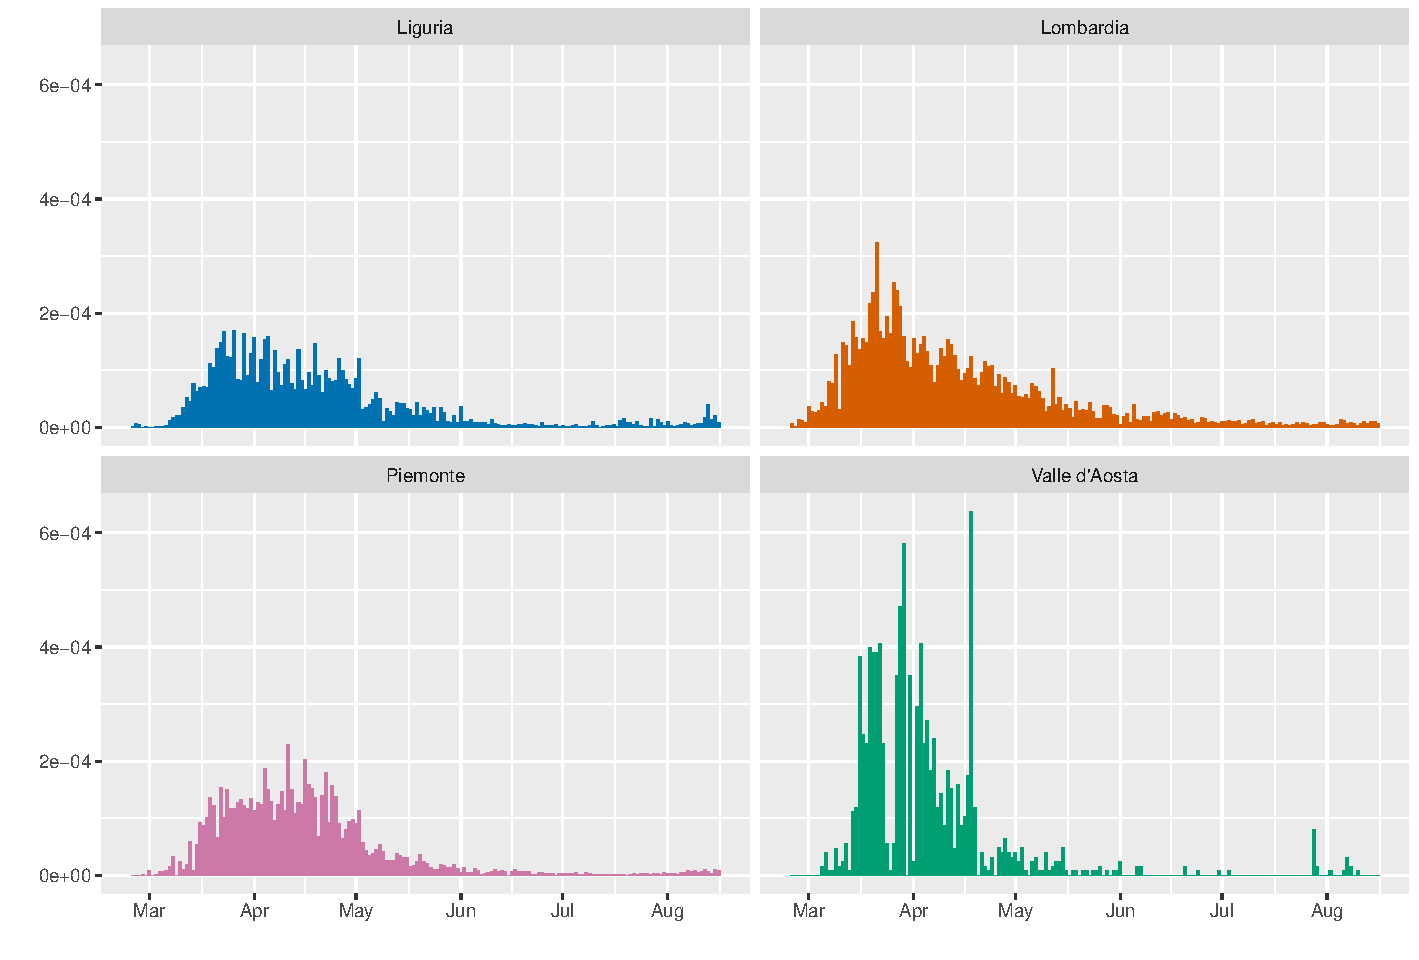
\includegraphics[width=0.92\textwidth]{output/infective_rates_Nord-Ovest.pdf}
    	    \caption{Incidence rate per region for the Nord-Ovest NUTS 1 region.}
    	    \label{fig:incidence_nordovest}
    	\end{figure}
    	
    	\begin{figure}[H]
    	    \centering
    	    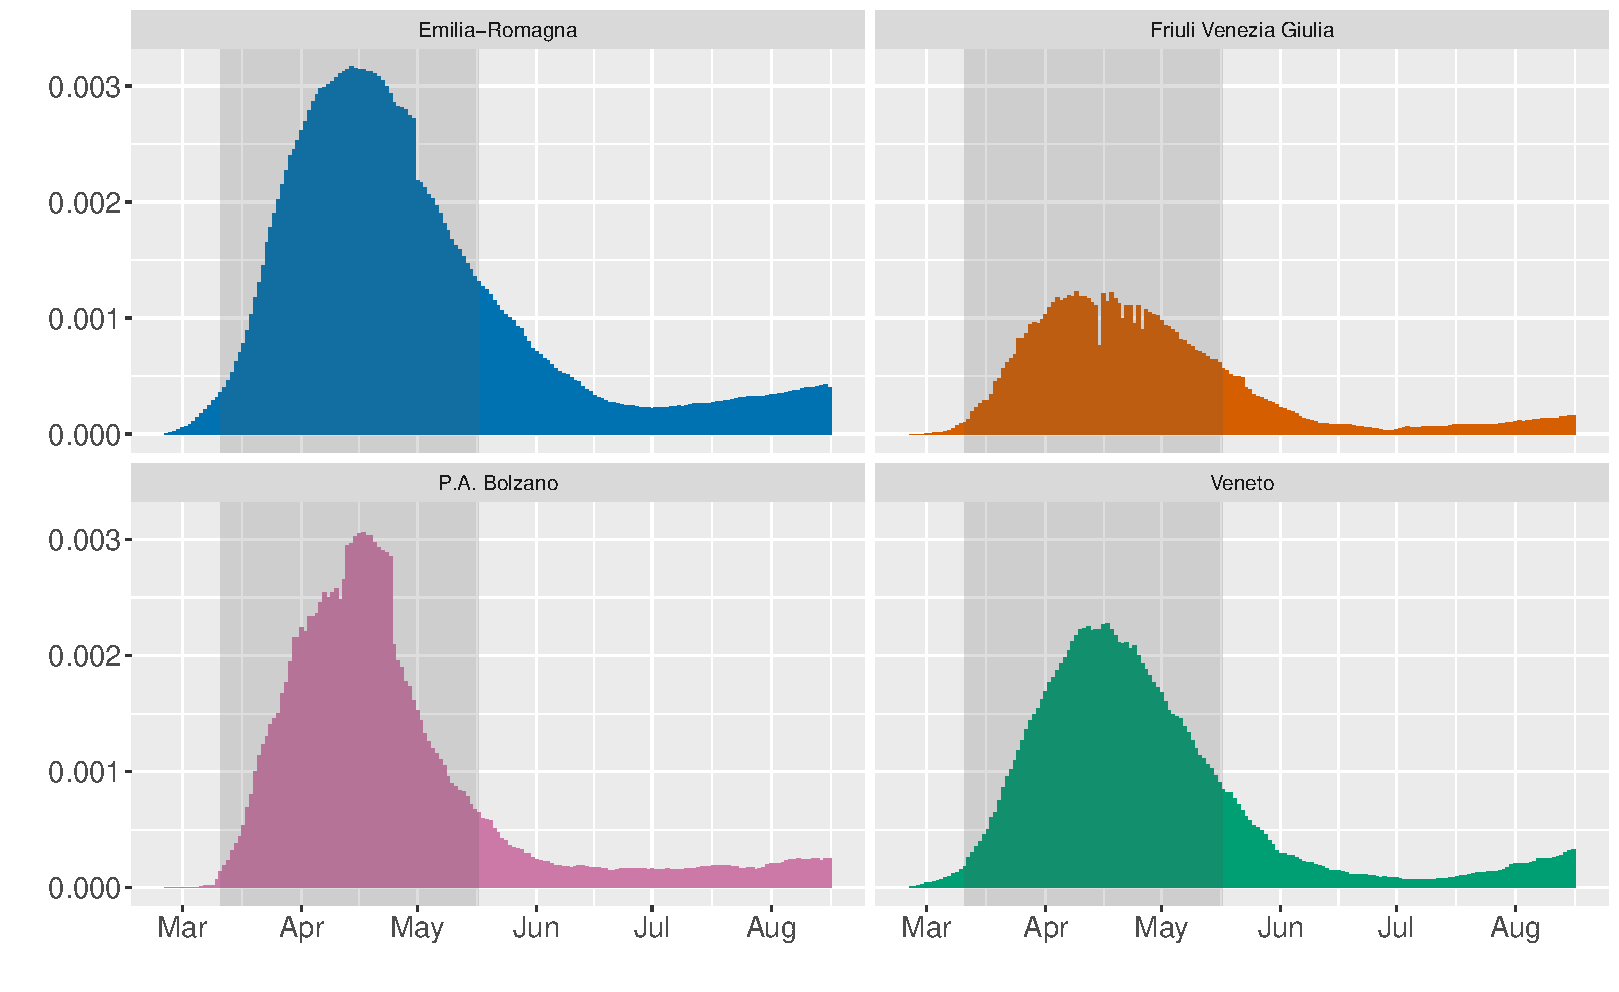
\includegraphics[width=0.92\textwidth]{output/infective_rates_Nord-Est.pdf}
    	    \caption{Incidence rate per region for the Nord-Est NUTS 1 region.}
    	    \label{fig:incidence_nordest}
    	\end{figure}
    	
    	\begin{figure}[H]
    	    \centering
    	    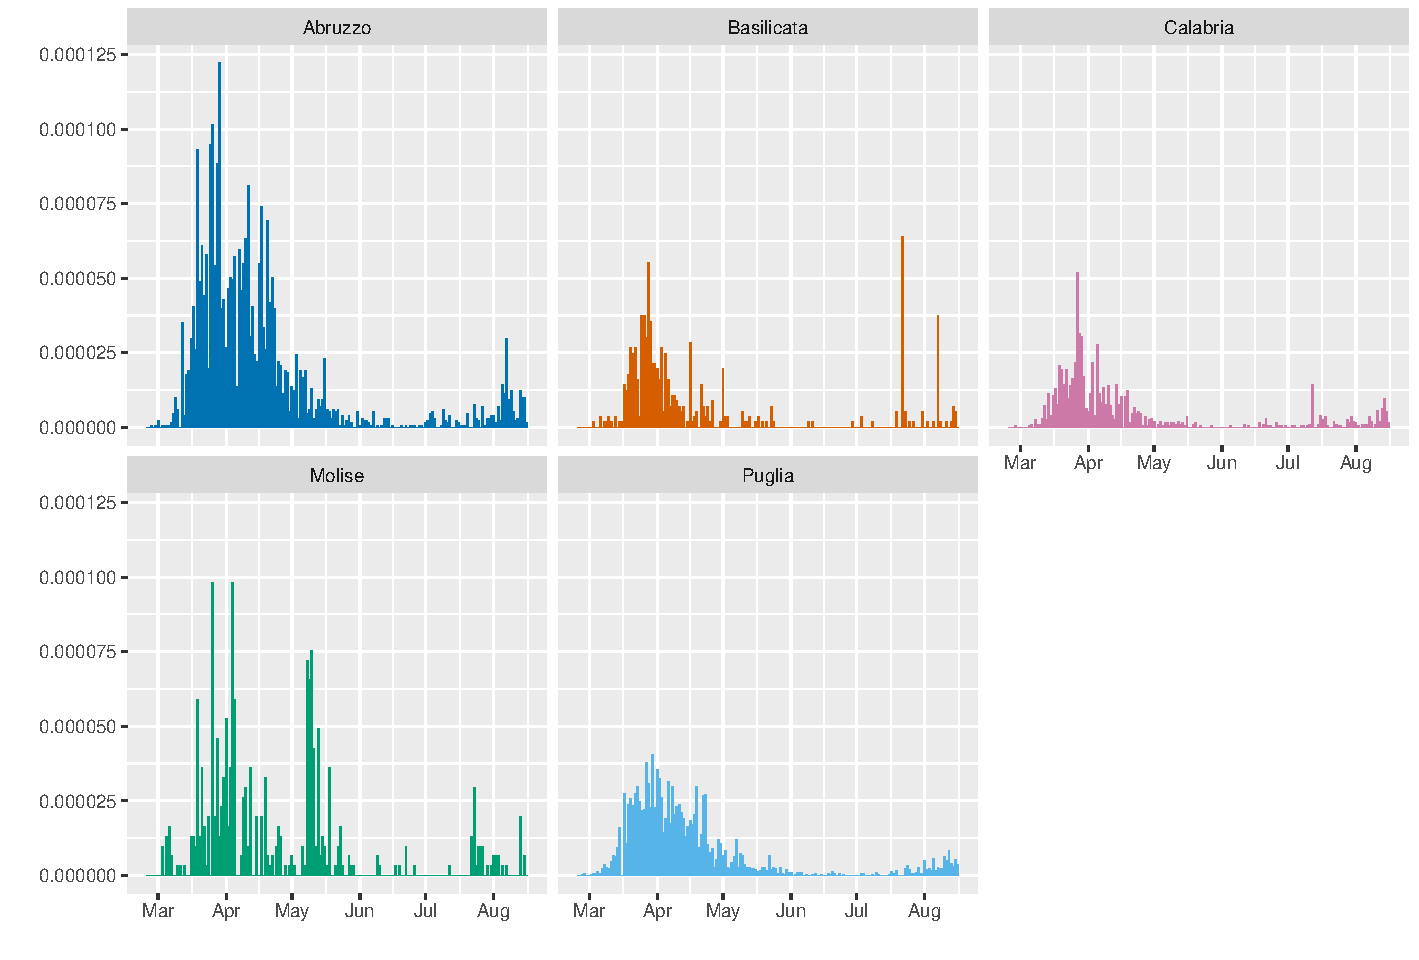
\includegraphics[width=0.92\textwidth]{output/infective_rates_Sud.pdf}
    	    \caption{Incidence rate per region for the Sud NUTS 1 region.}
    	    \label{fig:incidence_sud}
    	\end{figure}
    	
    	\begin{figure}[H]
    	    \centering
    	    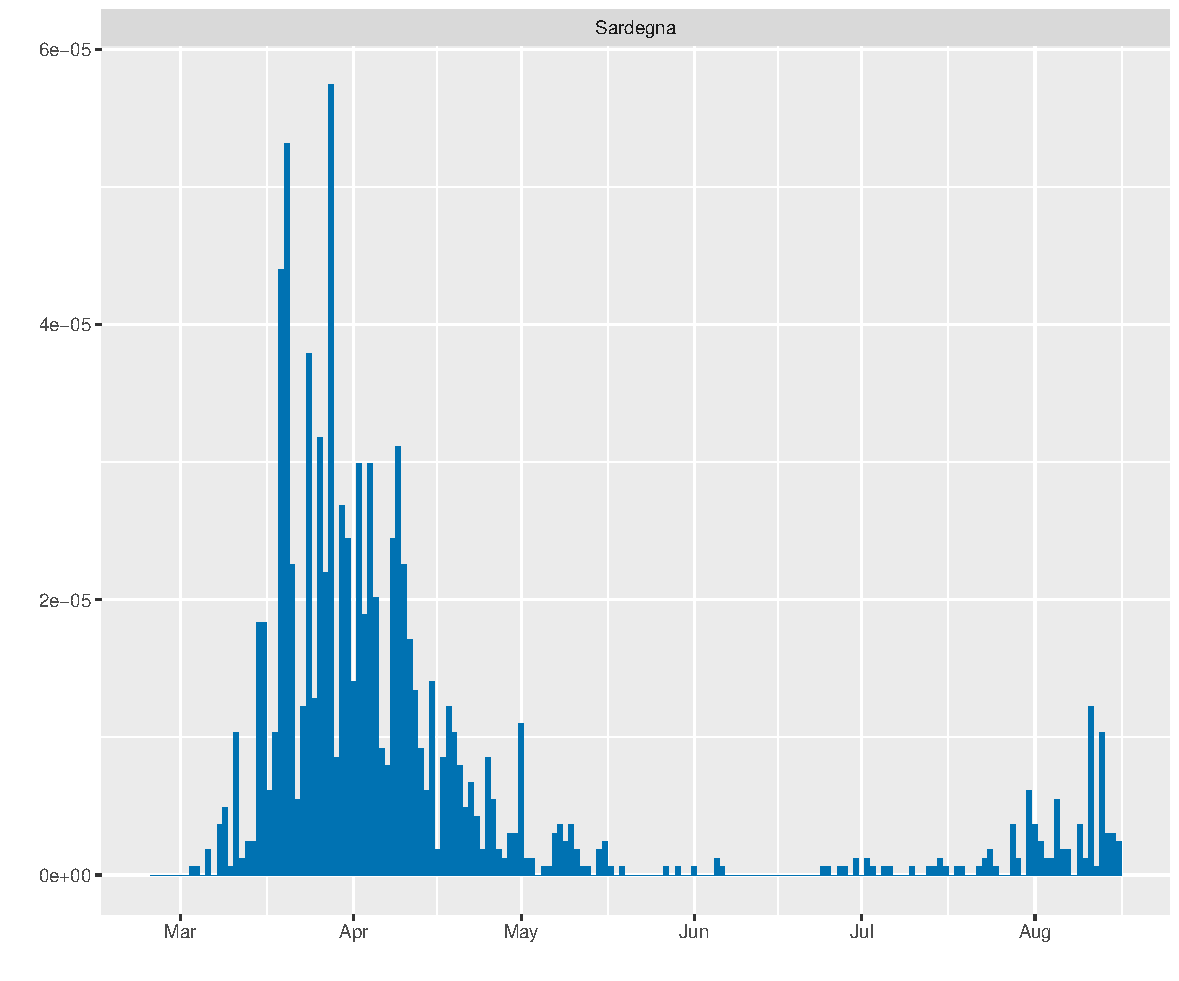
\includegraphics[width=0.7\textwidth]{output/infective_rates_Isole.pdf}
    	    \caption{Incidence rate per region for the Isole NUTS 1 region.}
    	    \label{fig:incidence_isole}
    	\end{figure}
		
% 		\subsection{Figures for Section \ref{sec:dataset}: \nameref{sec:dataset}} \label{sapp:figures_dataset}
% 		This appendix contains additional plots as referenced in Section \ref{sec:dataset}.
		
% 		\begin{figure}[H]
%     	    \centering
%     	    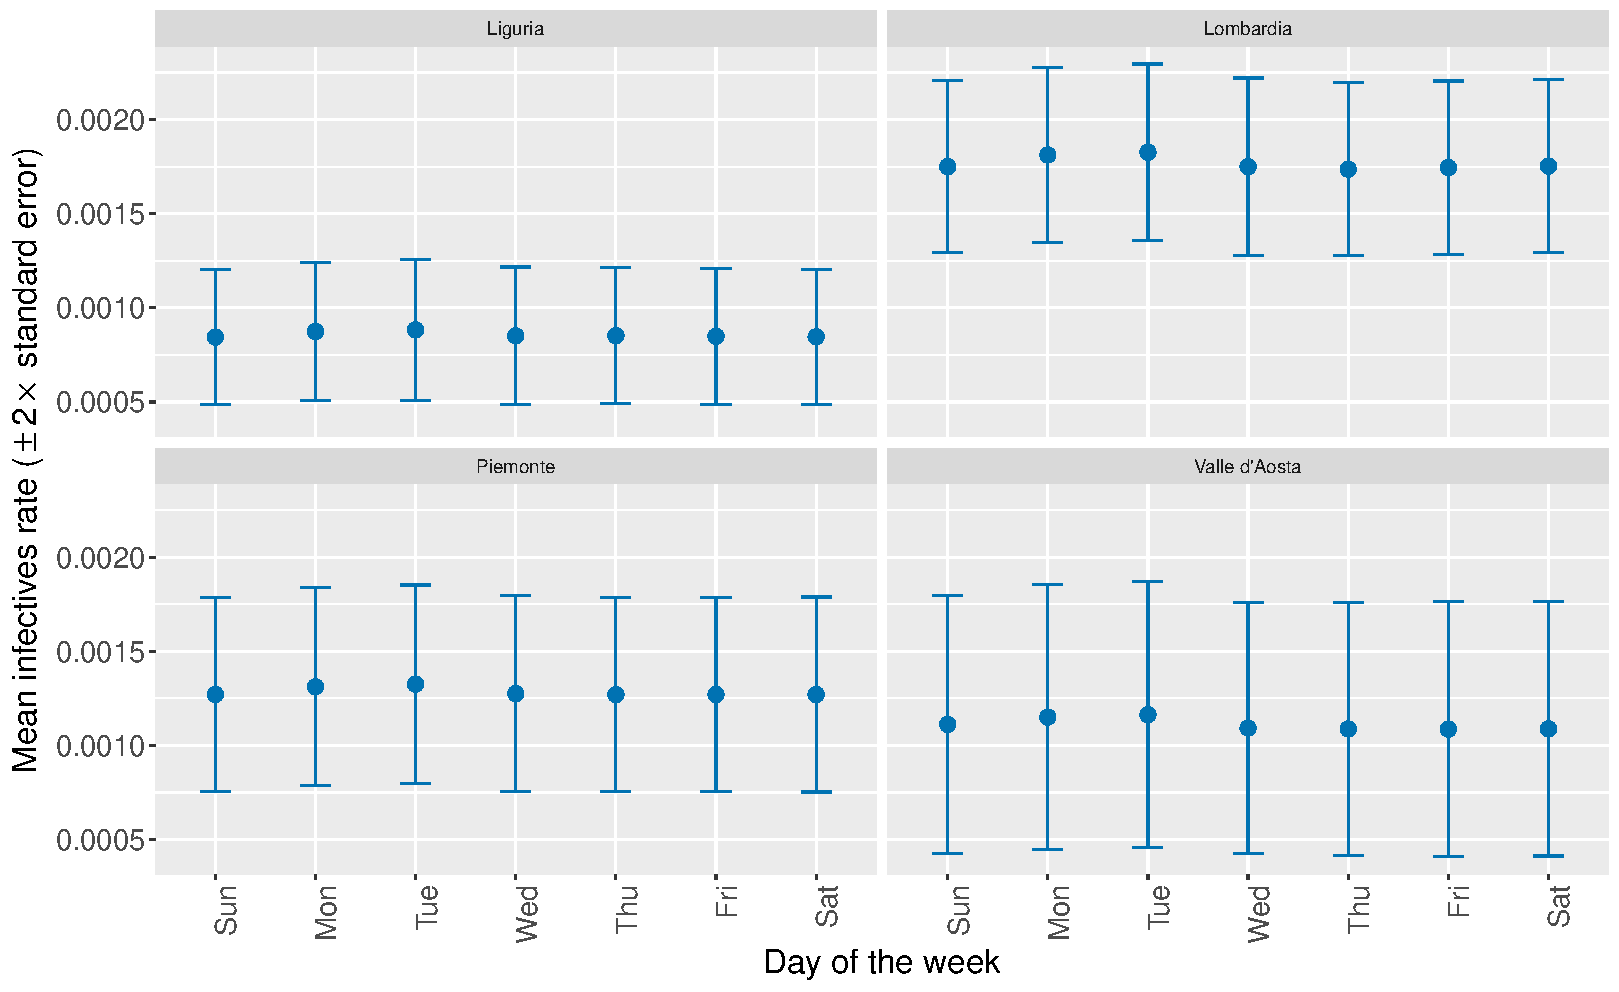
\includegraphics[width=0.92\textwidth]{output/infective_rates_weekday_Nord-Ovest.pdf}
%     	    \caption{Incidence rate per NUTS 2 region per day of the week for the Nord-Ovest NUTS 1 region}
%     	    \label{fig:incidence_nordovest_weekday}
%     	\end{figure}
		
% 		\begin{figure}[H]
%     	    \centering
%     	    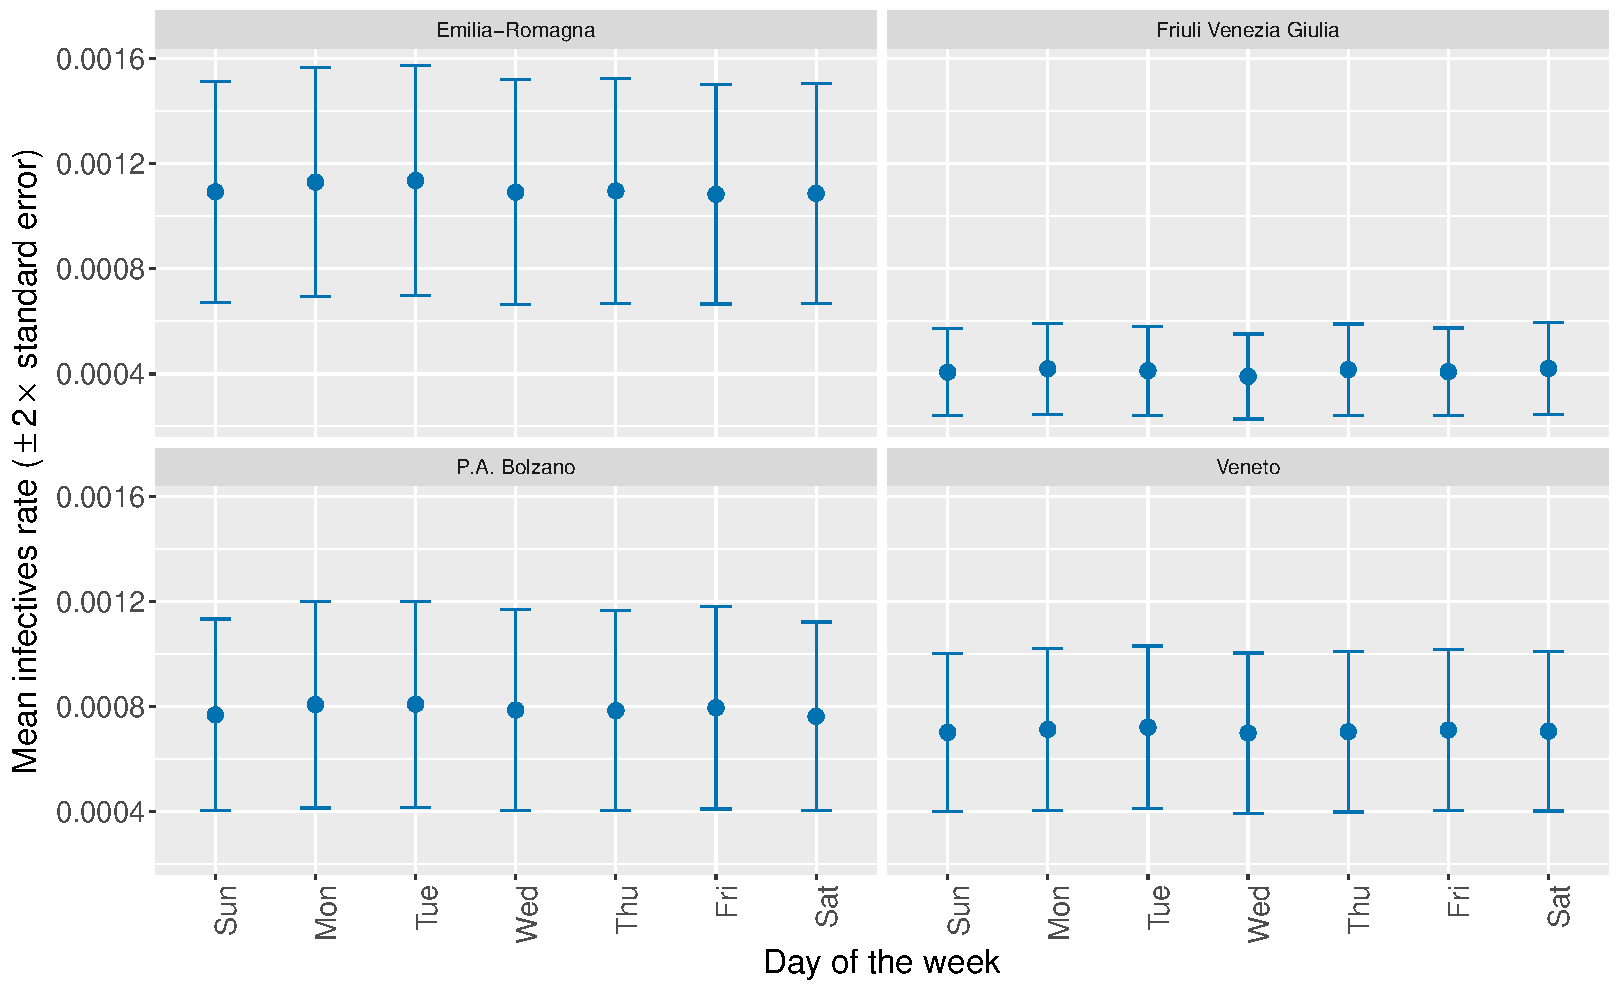
\includegraphics[width=0.92\textwidth]{output/infective_rates_weekday_Nord-Est.pdf}
%     	    \caption{Incidence rate per NUTS 2 region per day of the week for the Nord-Est NUTS 1 region}
%     	    \label{fig:incidence_nordest_weekday}
%     	\end{figure}
    	
%     	\begin{figure}[H]
%     	    \centering
%     	    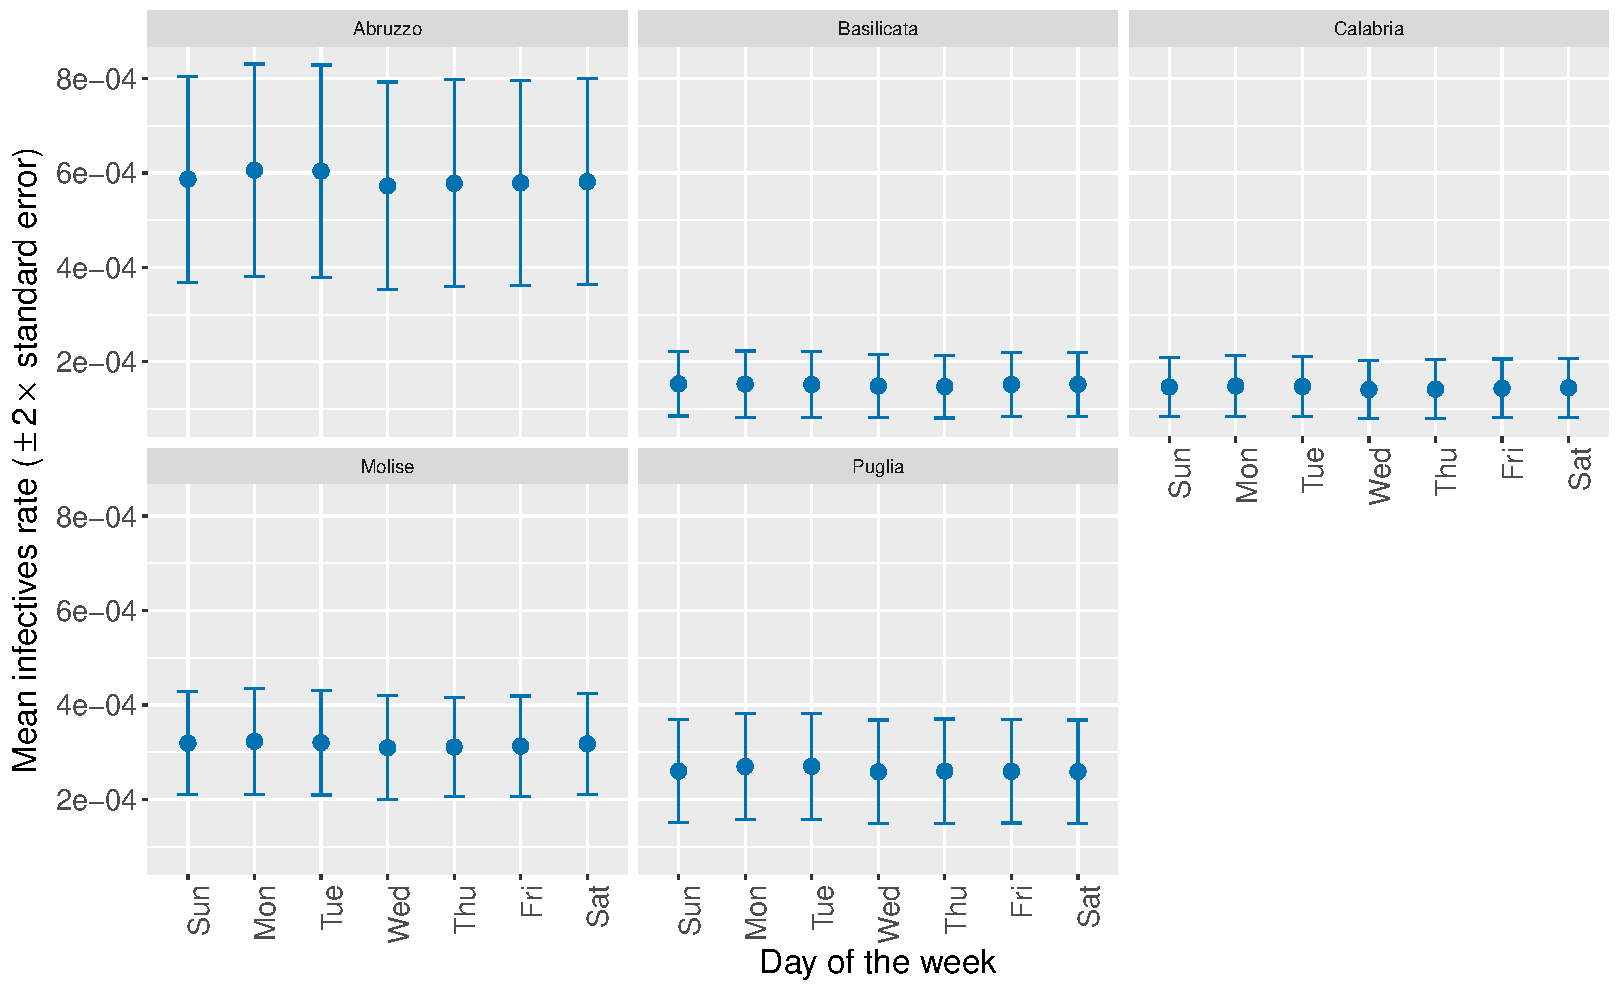
\includegraphics[width=0.92\textwidth]{output/infective_rates_weekday_Sud.pdf}
%     	    \caption{Incidence rate per NUTS 2 region per day of the week for the Sud NUTS 1 region}
%     	    \label{fig:incidence_sud_weekday}
%     	\end{figure}
		
% 		\begin{figure}[H]
%     	    \centering
%     	    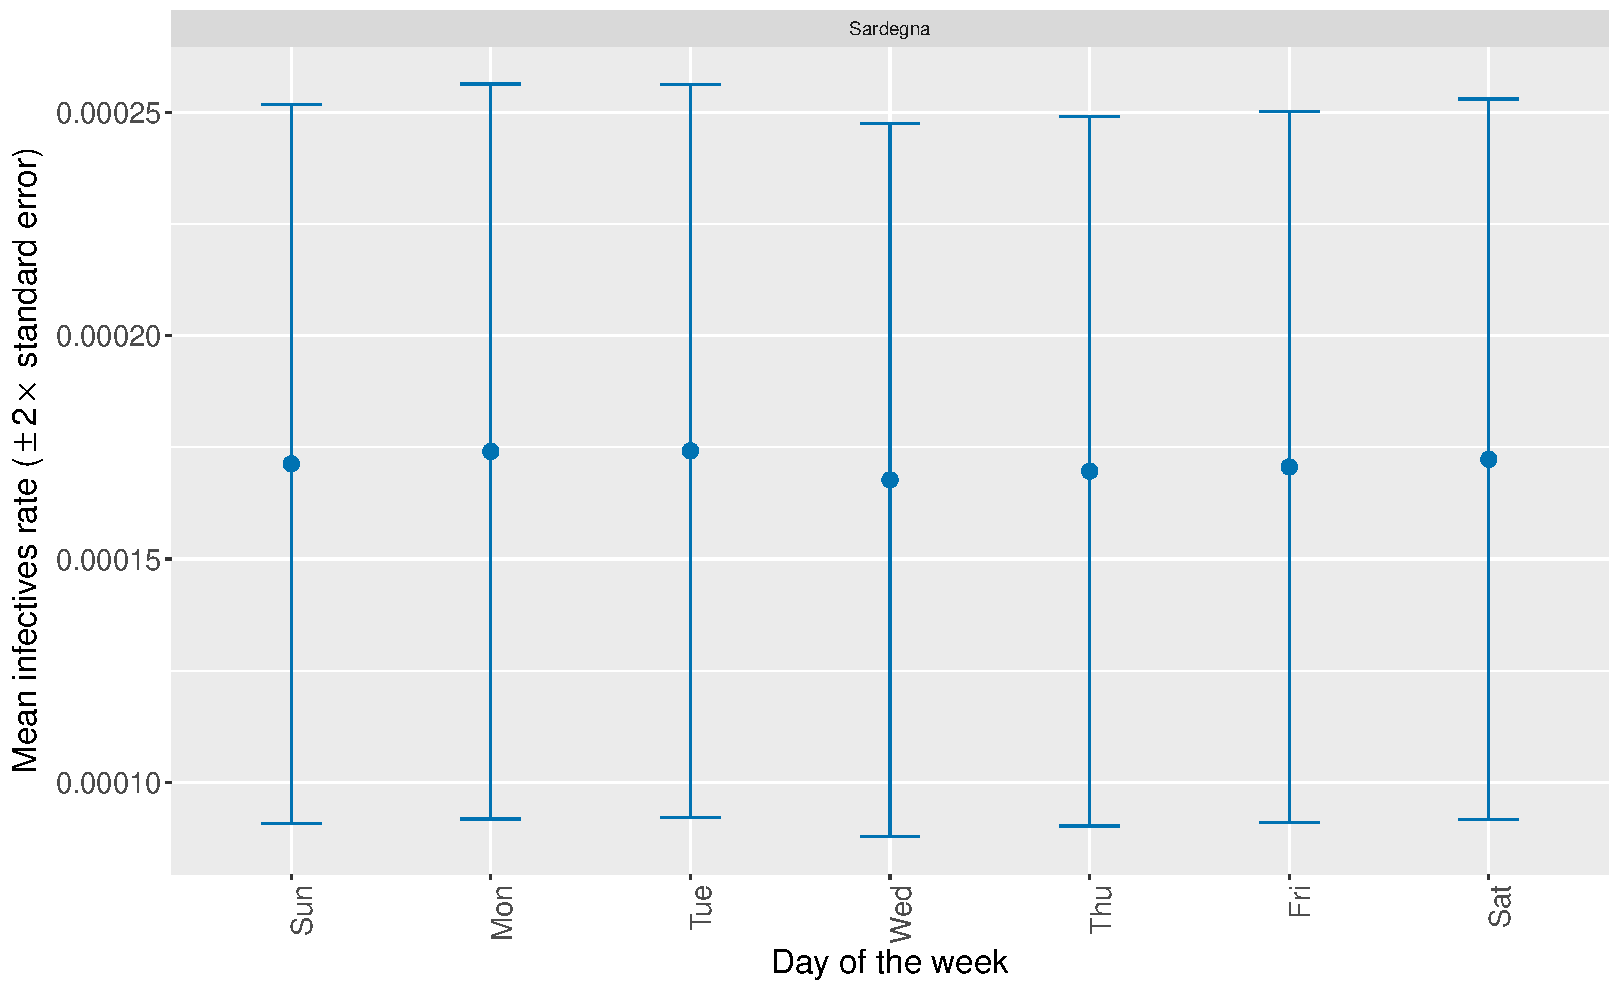
\includegraphics[width=0.7\textwidth]{output/infective_rates_weekday_Isole.pdf}
%     	    \caption{Incidence rate per NUTS 2 region per day of the week for the Isole NUTS 1 region}
%     	    \label{fig:incidence_isole_weekday}
%     	\end{figure}
		
		\newpage
		\subsection{Figures for the Within-Region Spread Model} \label{sapp:figures_model_within}
		In Section \ref{subsec:model_within_results} we presented the plots of $\beta_{within}$ over time for the Nord-Est NUTS 1 region for the within-region spread model. In this appendix, we present the plots for the other NUTS 1 regions. \\
		
		\begin{figure}[H]
    	    \centering
    	    \begin{subfigure}{\textwidth}
    	      \centering
    	      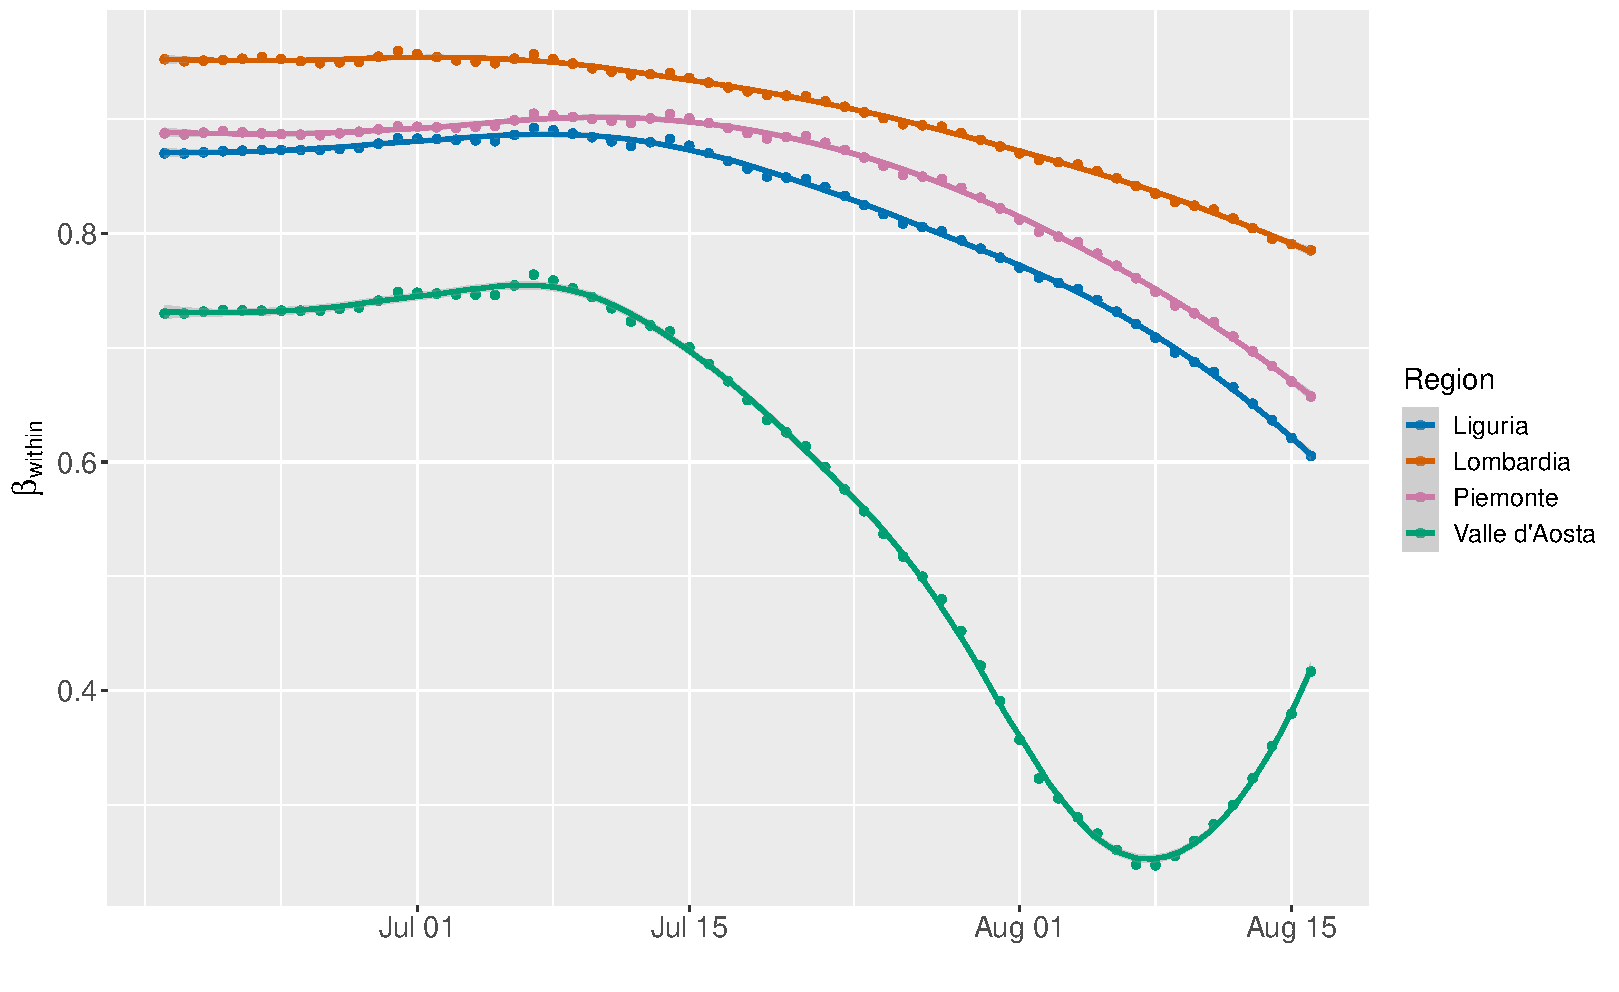
\includegraphics[width=0.91\linewidth]{output/model_within_lag14_betawithin_Nord-Ovest_rolling.pdf}
    	      \caption{Without model selection}
    	      \label{fig:beta_within_over_time_northwest_regular}
    	    \end{subfigure}\newline
    	    \begin{subfigure}{\textwidth}
    	      \centering
    	      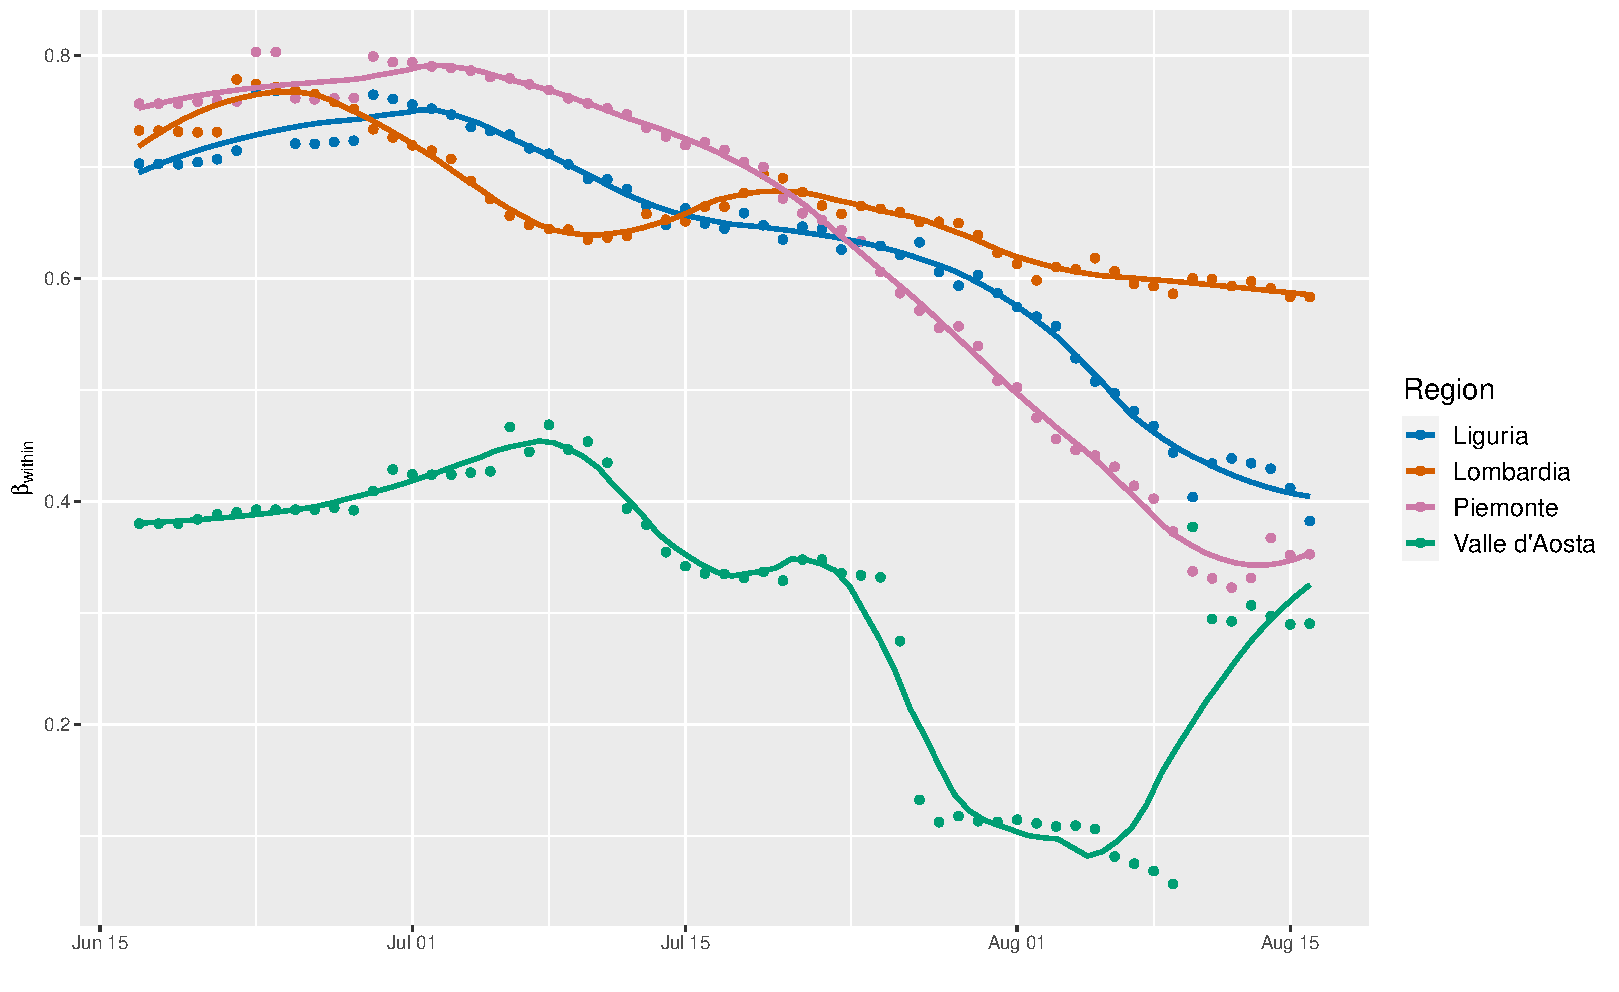
\includegraphics[width=0.91\linewidth]{output/model_within_lag14_betawithin_Nord-Ovest_aic_rolling.pdf}
    	      \caption{With model selection by AIC}
    	      \label{fig:beta_within_over_time_northwest_aic}
    	    \end{subfigure}
        \end{figure}
        \begin{figure}[H]\ContinuedFloat
    	    \begin{subfigure}{\textwidth}
    	      \centering
    	      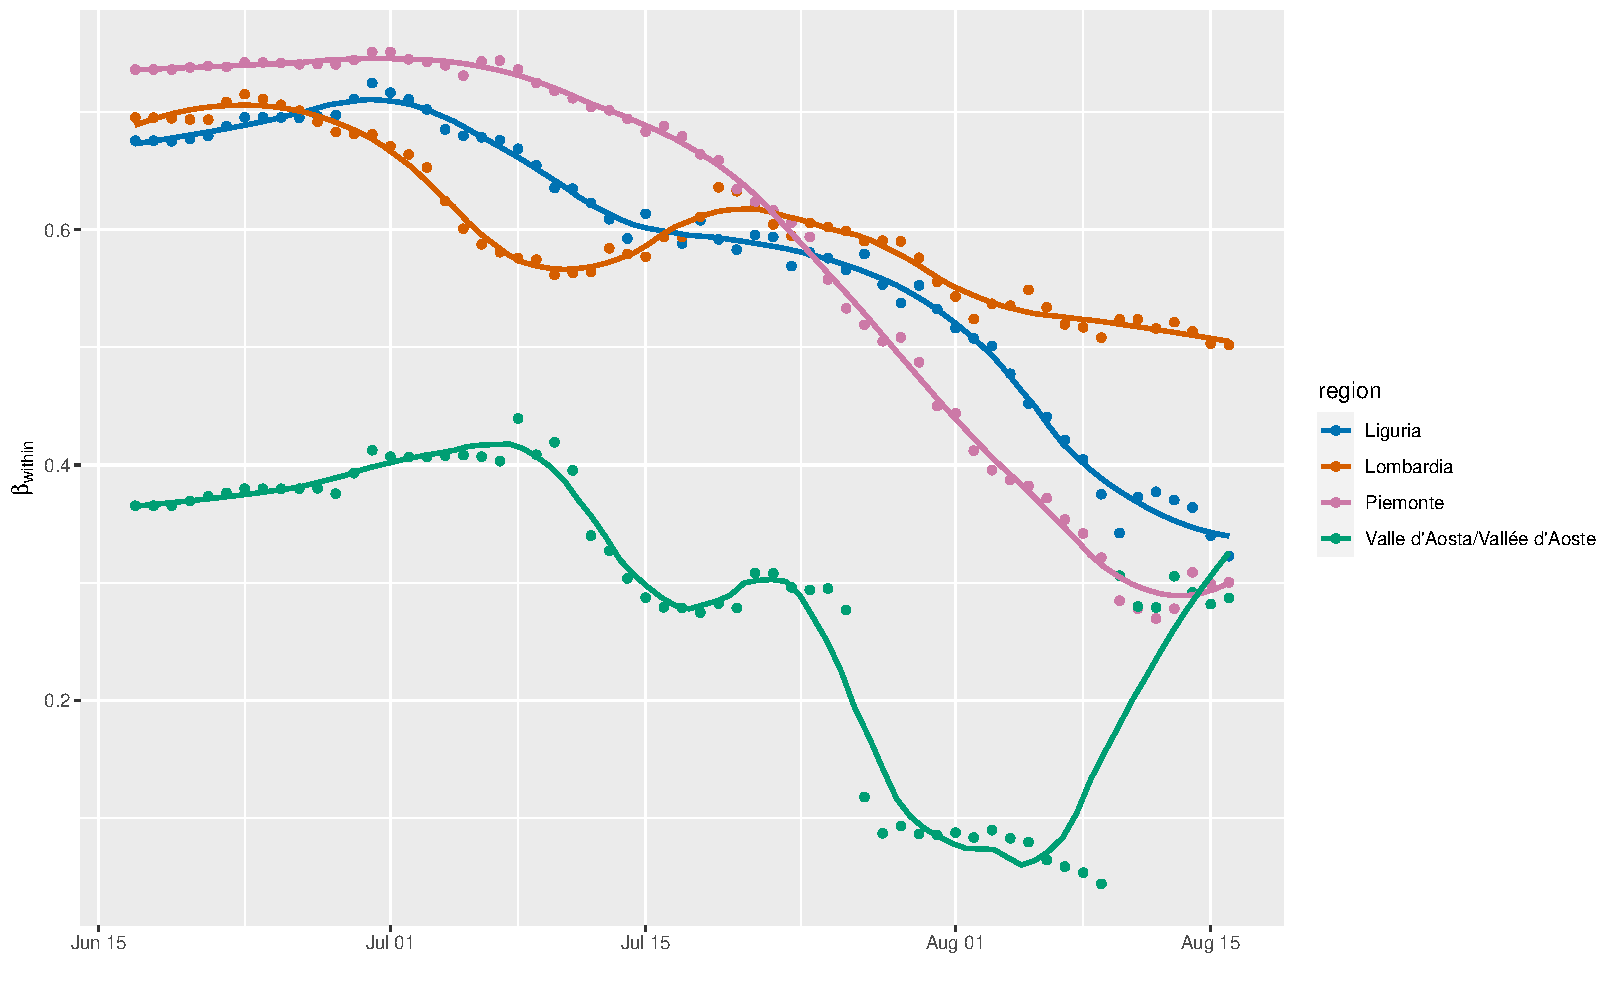
\includegraphics[width=0.92\linewidth]{output/model_within_lag14_betawithin_Nord-Ovest_UndocQuadratic_rolling.pdf}
    	      \caption{Without model selection; \\ including undocumented infectives}
    	      \label{fig:beta_within_over_time_northwest_regular_undoc}
    	    \end{subfigure}\newline
    	    \begin{subfigure}{\textwidth}
    	      \centering
    	      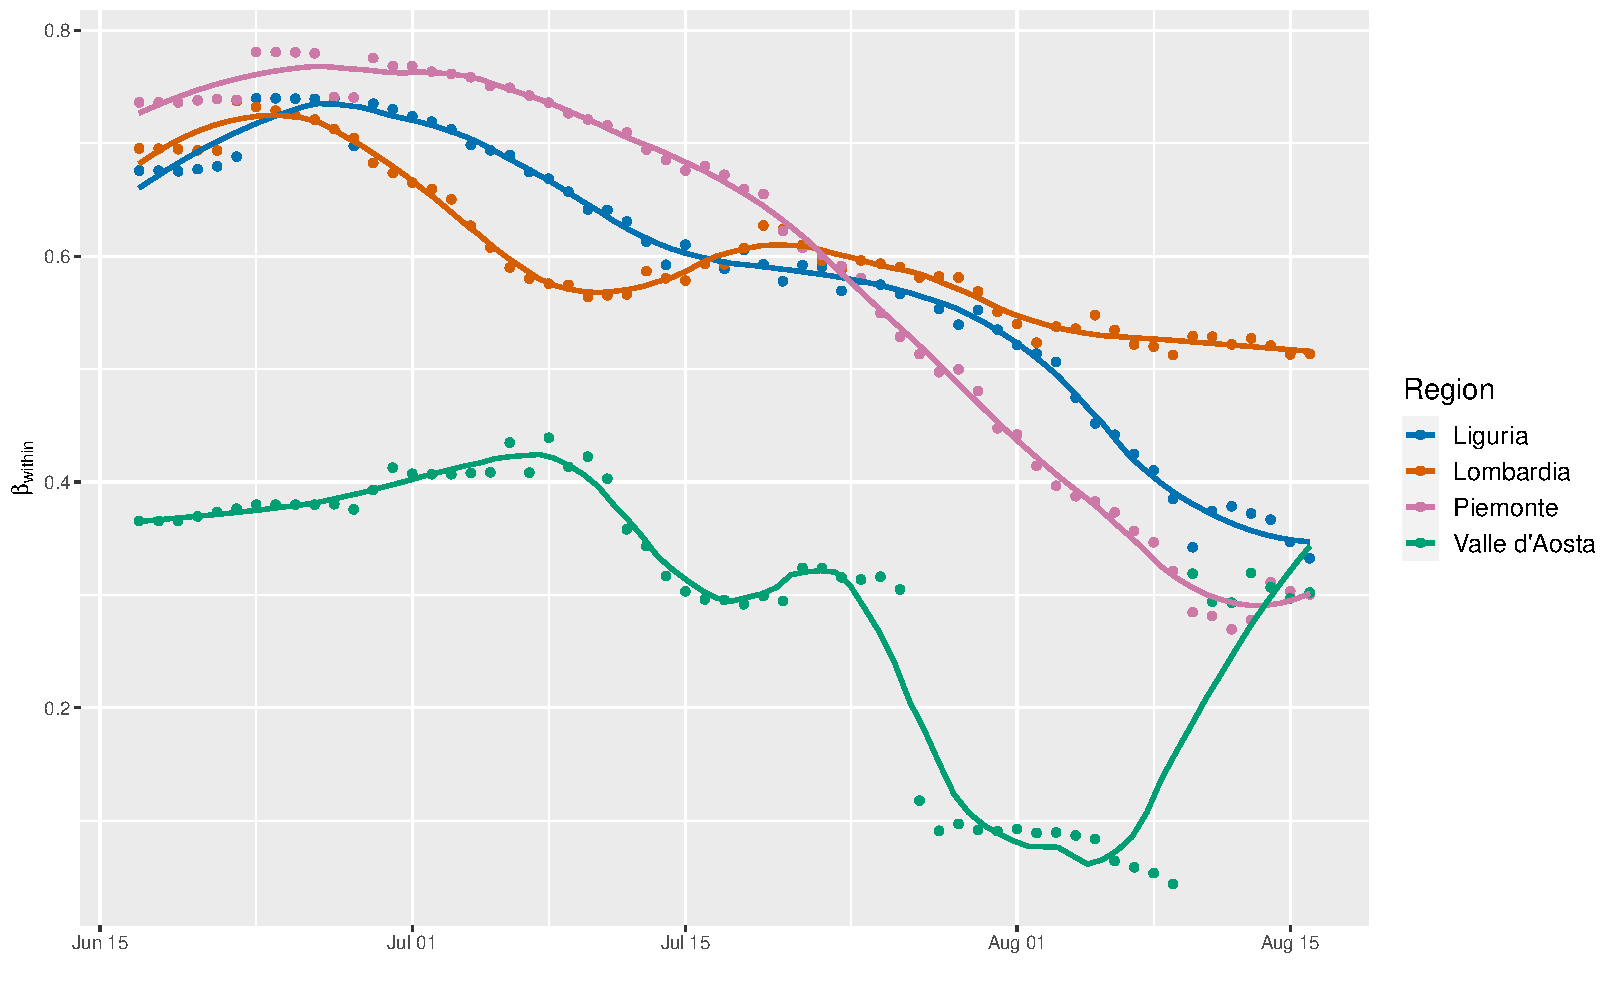
\includegraphics[width=0.92\linewidth]{output/model_within_lag14_betawithin_Nord-Ovest_aic_UndocQuadratic_rolling.pdf}
    	      \caption{With model selection by AIC; \\ including undocumented infectives}
    	      \label{fig:beta_within_over_time_northwest_aic_undoc}
    	    \end{subfigure}
    	    \caption{Progression of $\beta_{within}$ over time for the Nord-Ovest NUTS 1 region. Data spans May 9 until August 16, 2020 (100 days). Undocumented infectives are modelled using the quadratic specification with $\gamma = 0.7$ and $f^{min}=0.1$.}
    	    \label{fig:beta_within_over_time_northwest}
    	\end{figure}
		
		\begin{figure}[H]
    	    \centering
    	    \begin{subfigure}{\textwidth}
    	      \centering
    	      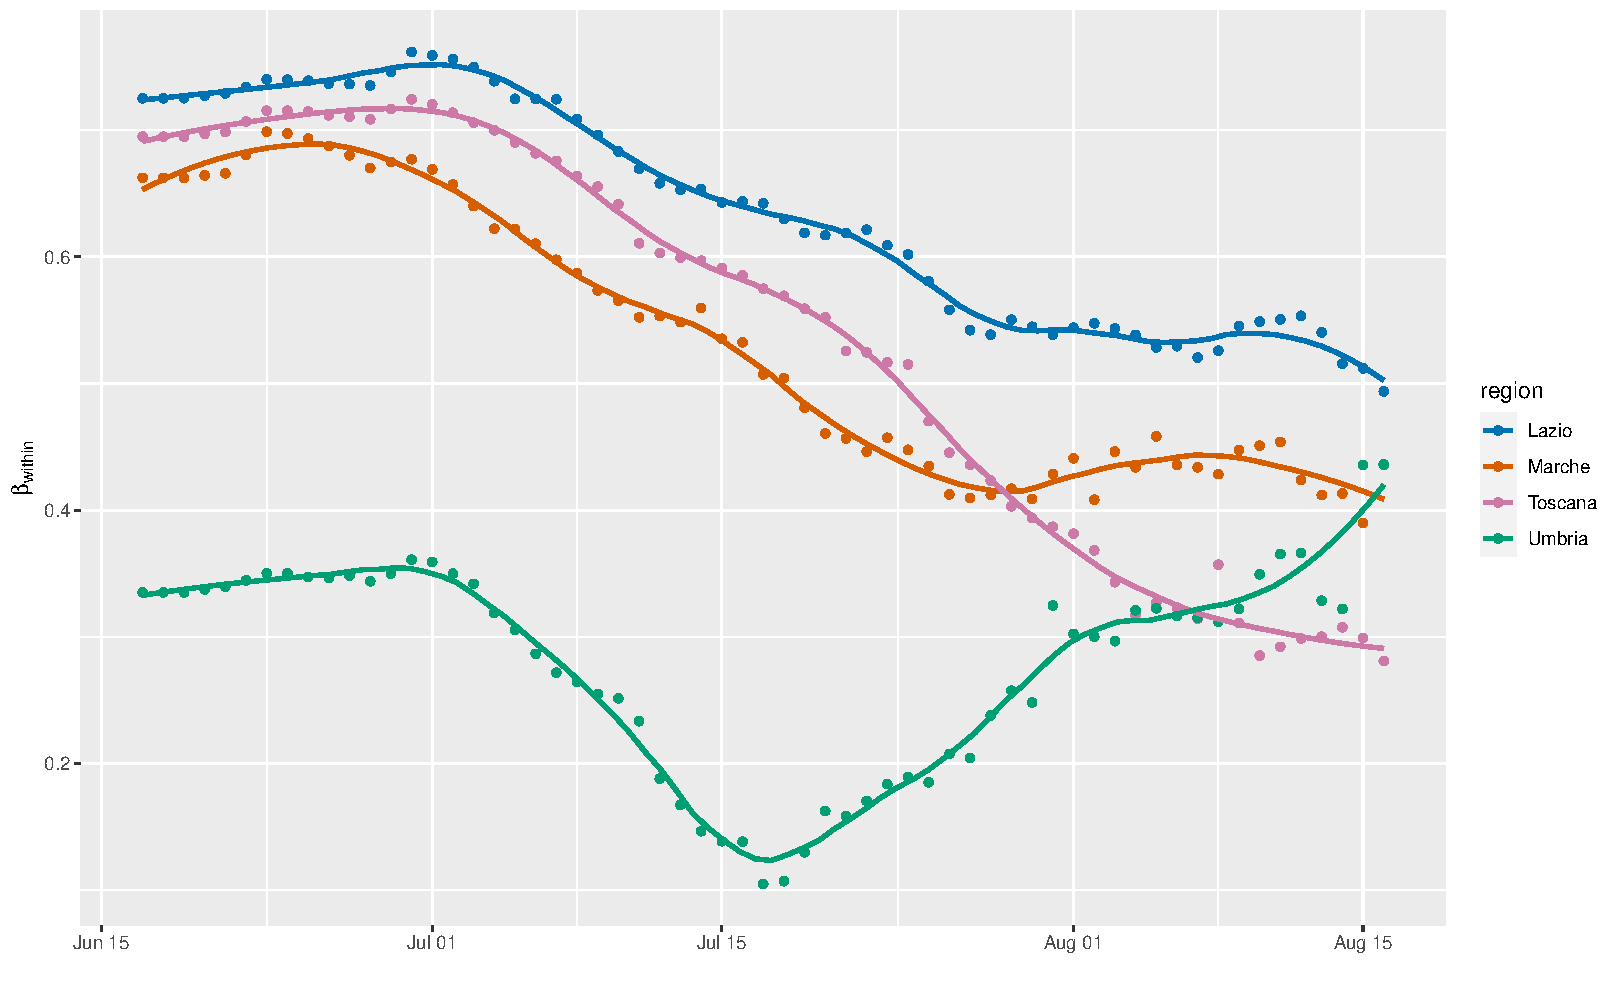
\includegraphics[width=0.92\linewidth]{output/model_within_lag14_betawithin_Centro (IT)_rolling.pdf}
    	      \caption{Without model selection}
    	      \label{fig:beta_within_over_time_centro_regular}
    	    \end{subfigure}\newline
    	    \begin{subfigure}{\textwidth}
    	      \centering
    	      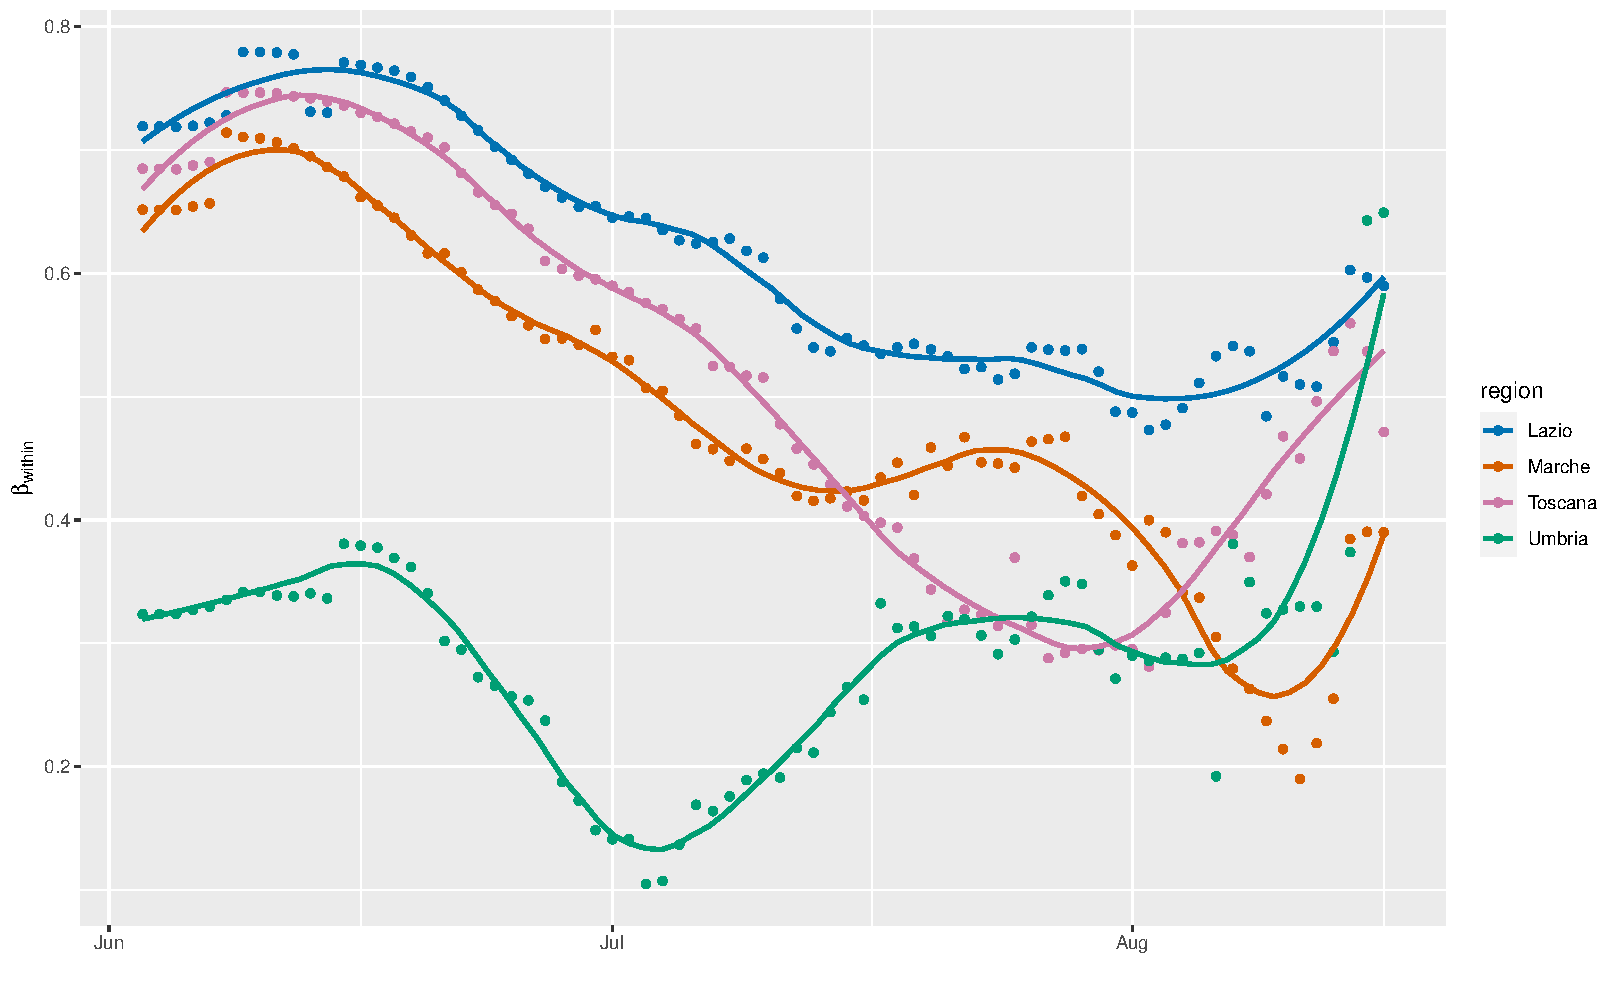
\includegraphics[width=0.92\linewidth]{output/model_within_lag14_betawithin_Centro (IT)_aic_rolling.pdf}
    	      \caption{With model selection by AIC}
    	      \label{fig:beta_within_over_time_centro_aic}
    	    \end{subfigure}
    	\end{figure}
        \begin{figure}[H]\ContinuedFloat
    	    \begin{subfigure}{\textwidth}
    	      \centering
    	      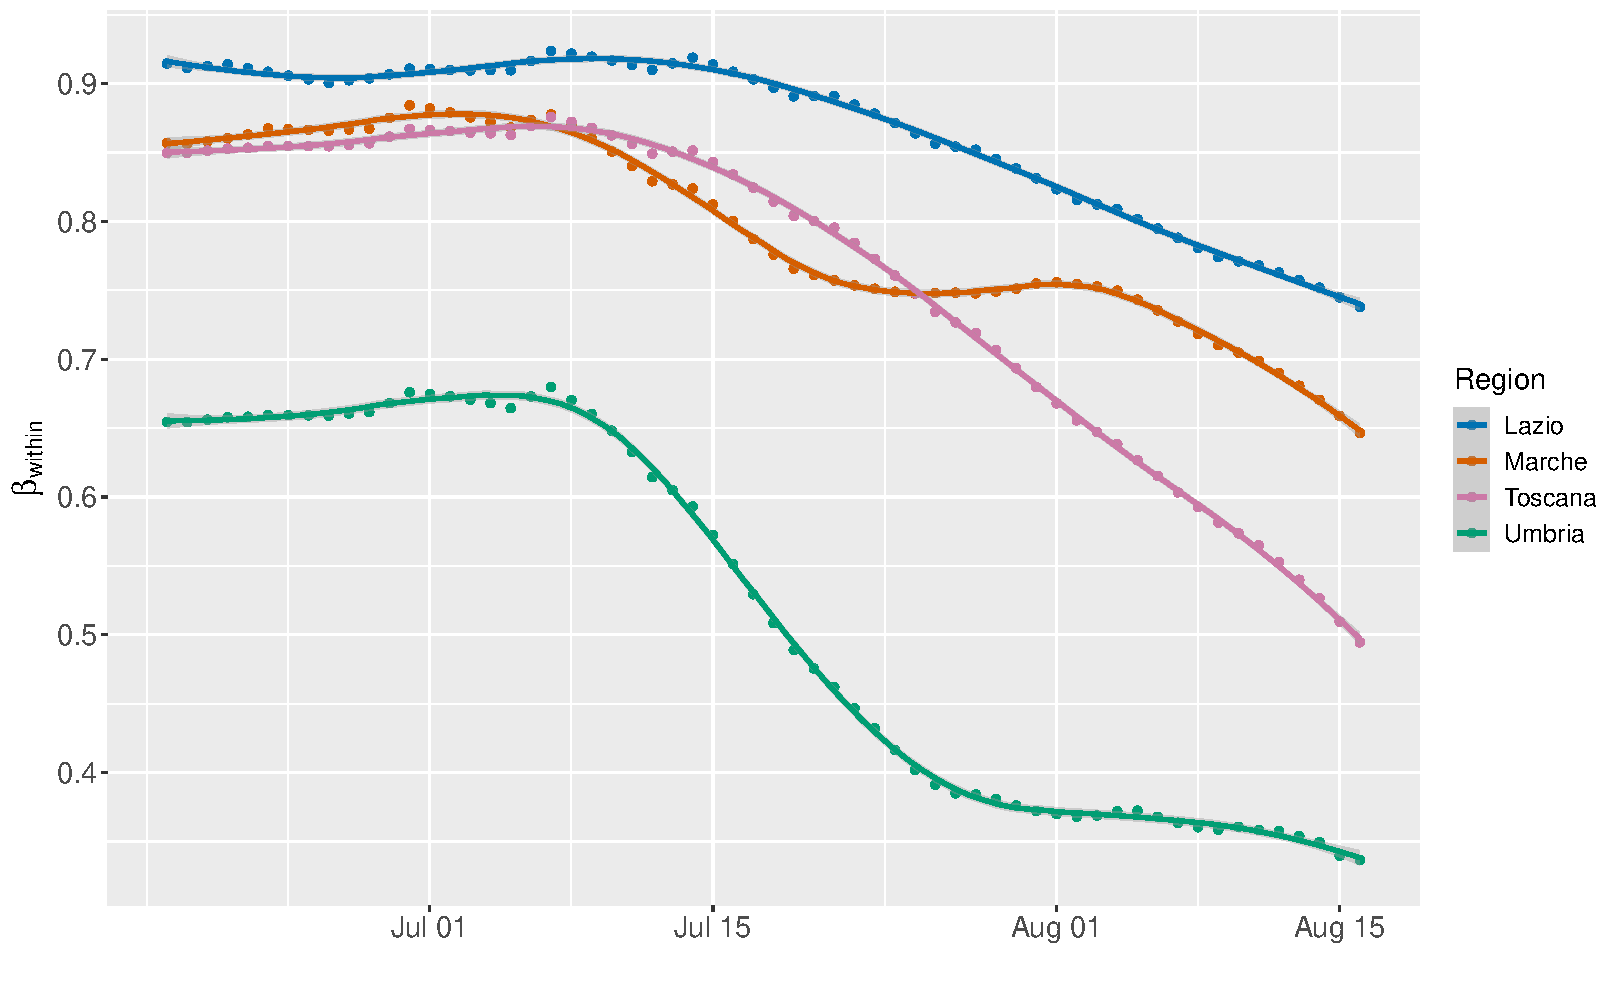
\includegraphics[width=0.92\linewidth]{output/model_within_lag14_betawithin_Centro (IT)_UndocQuadratic_rolling.pdf}
    	      \caption{Without model selection; \\ including undocumented infectives}
    	      \label{fig:beta_within_over_time_centro_regular_undoc}
    	    \end{subfigure}\newline
    	    \begin{subfigure}{\textwidth}
    	      \centering
    	      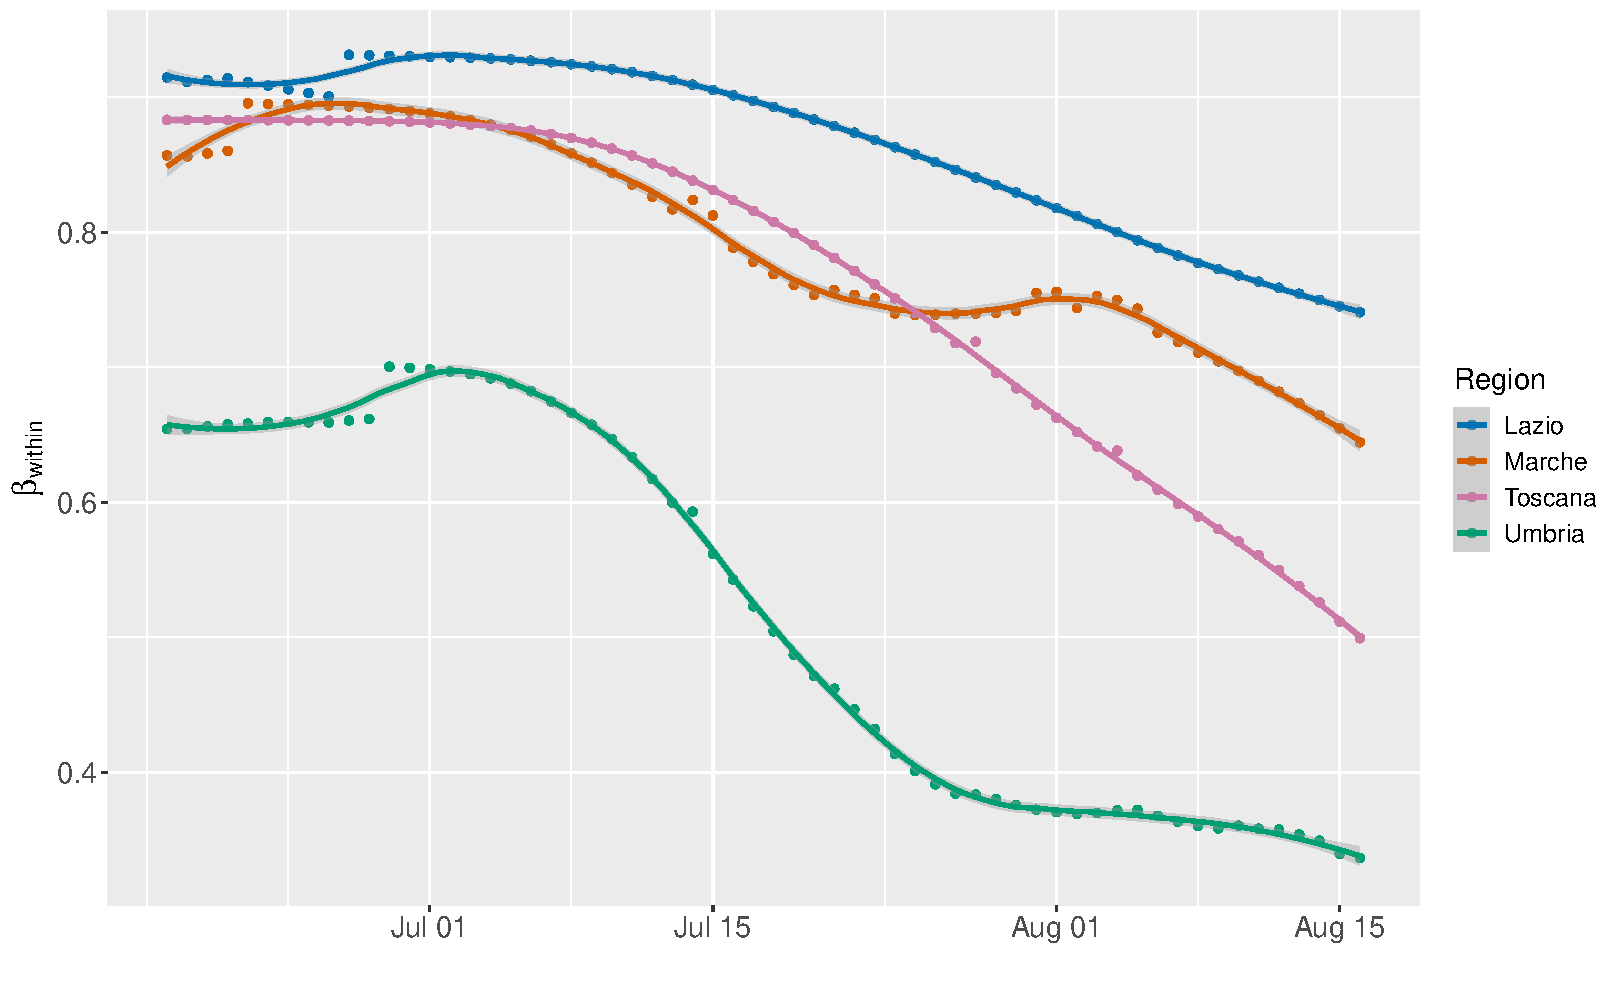
\includegraphics[width=0.92\linewidth]{output/model_within_lag14_betawithin_Centro (IT)_aic_UndocQuadratic_rolling.pdf}
    	      \caption{With model selection by AIC; \\ including undocumented infectives}
    	      \label{fig:beta_within_over_time_centro_aic_undoc}
    	    \end{subfigure}
    	    \caption{Progression of $\beta_{within}$ over time for the Centro (IT) NUTS 1 region. Data spans May 9 until August 16, 2020 (100 days). Undocumented infectives are modelled using the quadratic specification with $\gamma = 0.7$ and $f^{min}=0.1$.}
    	    \label{fig:beta_within_over_time_centro}
	    \end{figure}
		
		\begin{figure}[H]
    	    \centering
    	    \begin{subfigure}{\textwidth}
    	      \centering
    	      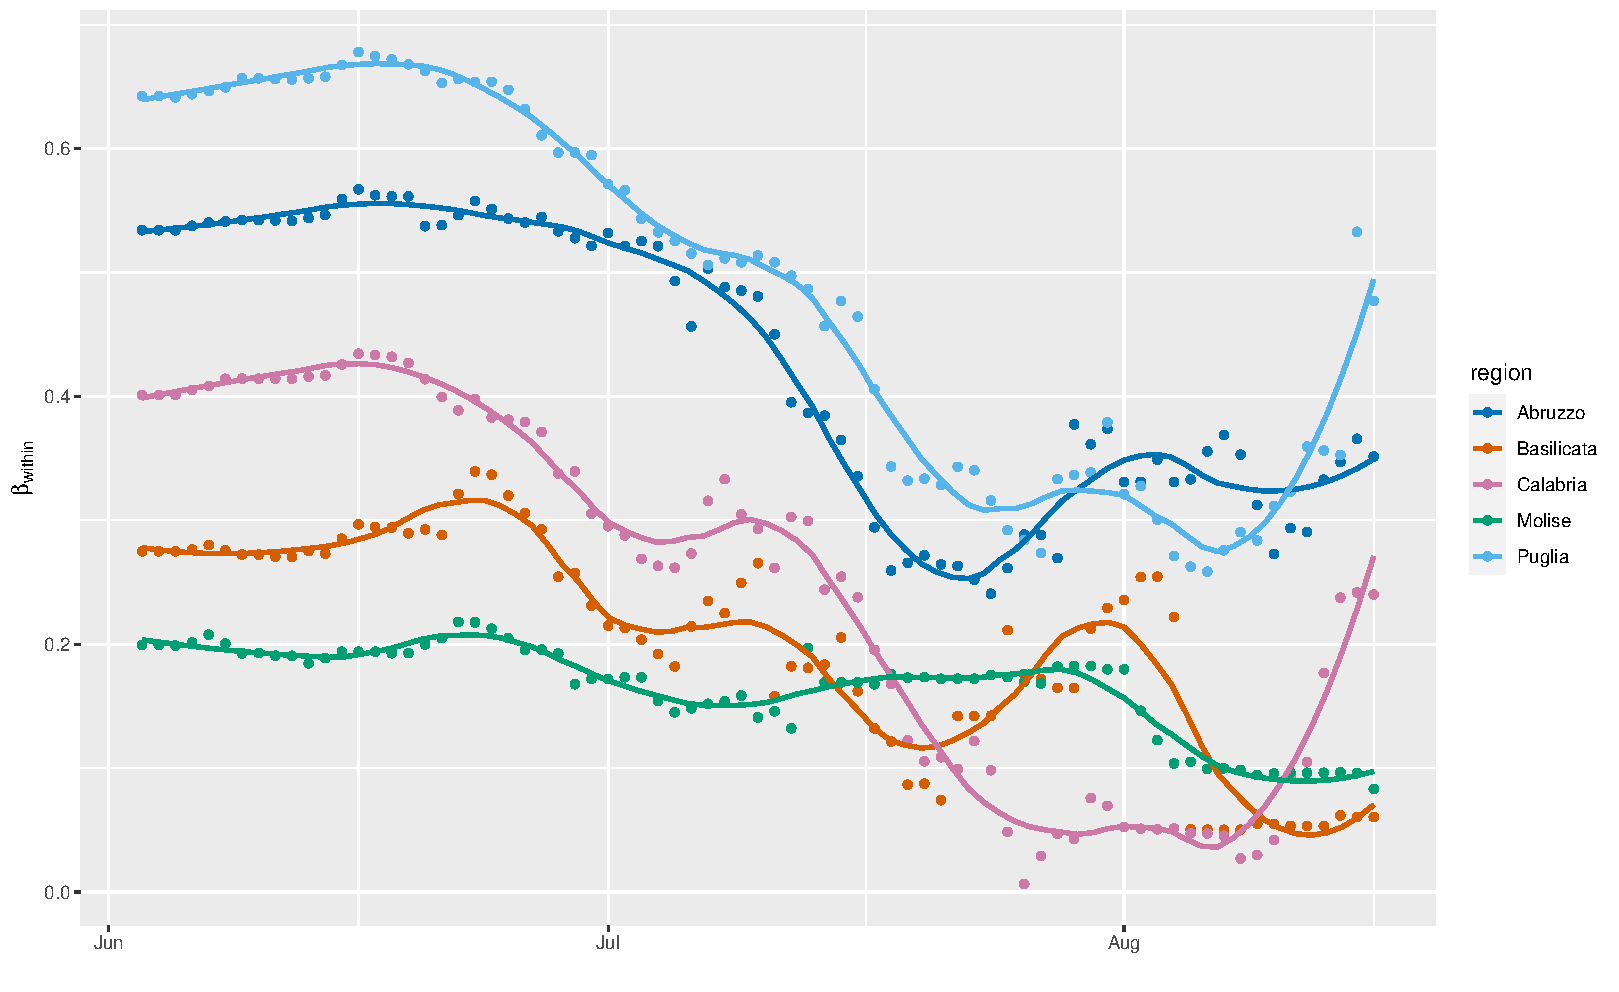
\includegraphics[width=0.92\linewidth]{output/model_within_lag14_betawithin_Sud_rolling.pdf}
    	      \caption{Without model selection}
    	      \label{fig:beta_within_over_time_sud_regular}
    	    \end{subfigure}\newline
    	    \begin{subfigure}{\textwidth}
    	      \centering
    	      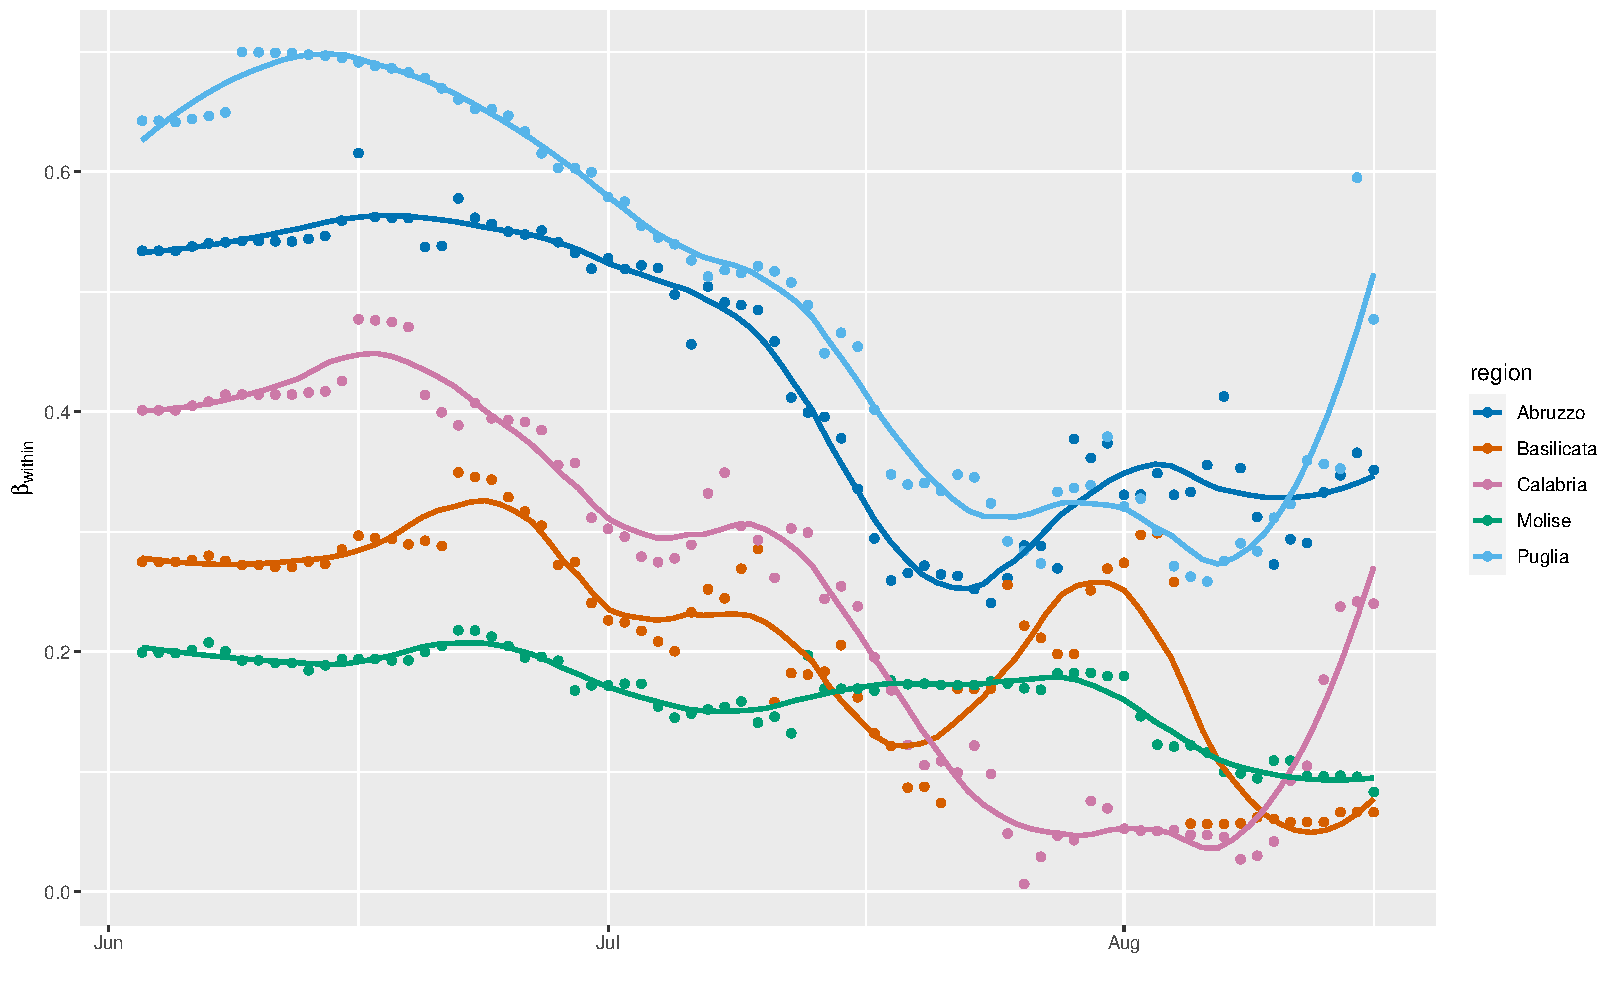
\includegraphics[width=0.92\linewidth]{output/model_within_lag14_betawithin_Sud_aic_rolling.pdf}
    	      \caption{With model selection by AIC}
    	      \label{fig:beta_within_over_time_sud_aic}
    	    \end{subfigure}
    	\end{figure}
        \begin{figure}[H]\ContinuedFloat
    	    \begin{subfigure}{\textwidth}
    	      \centering
    	      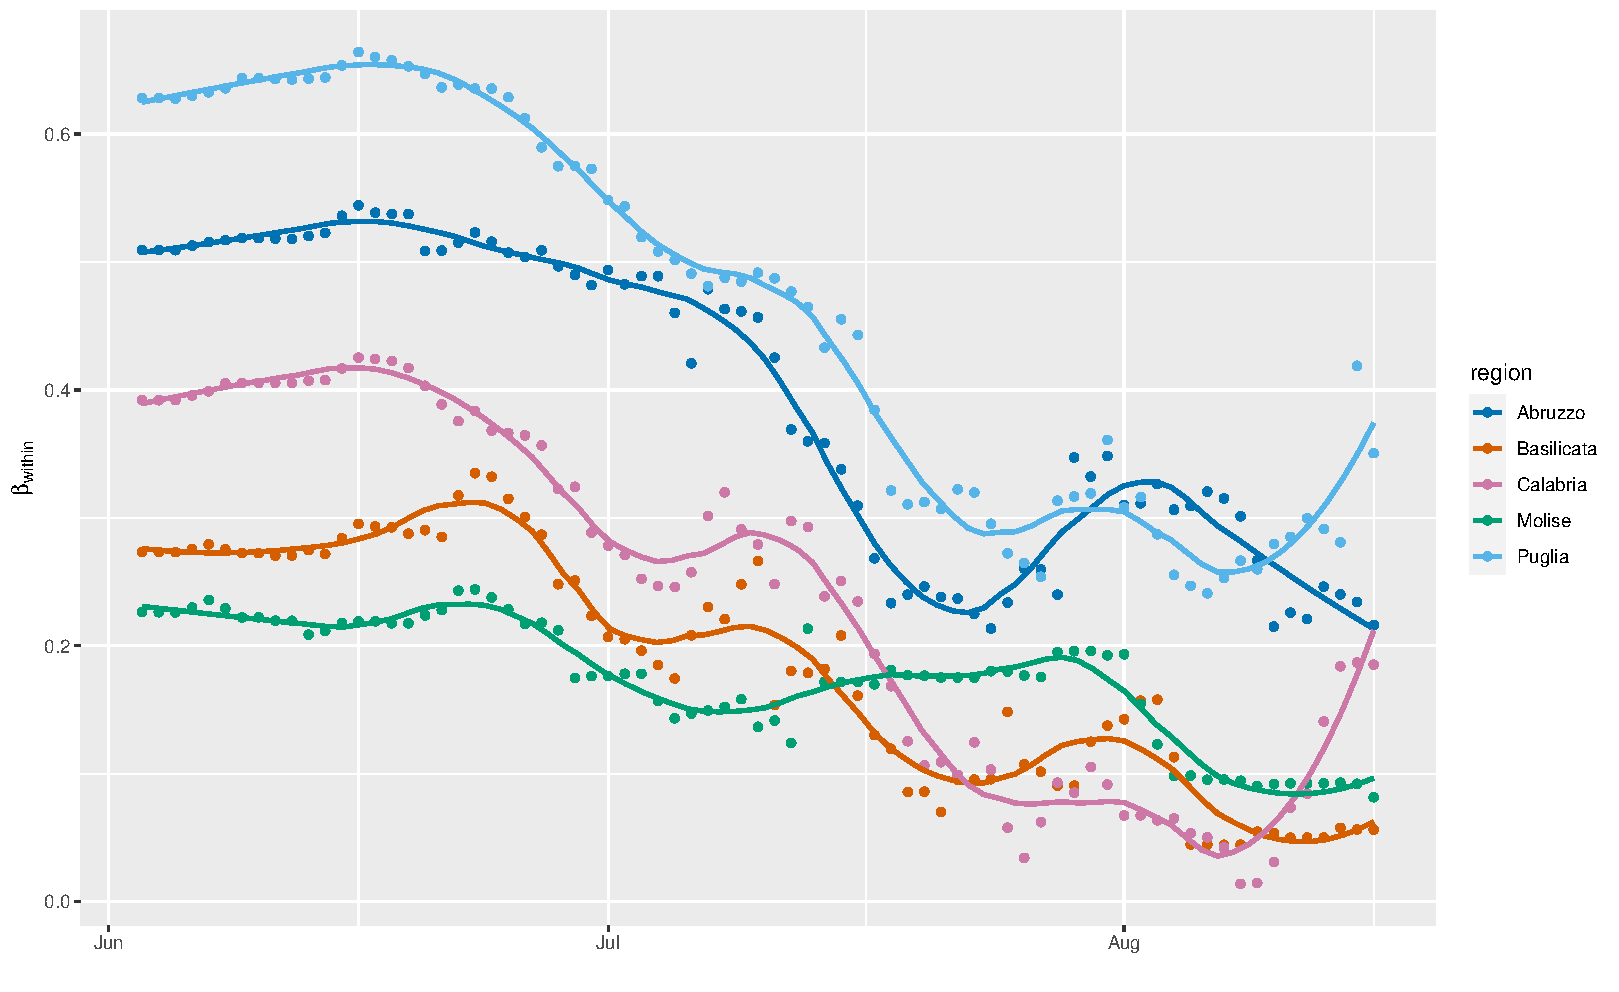
\includegraphics[width=0.92\linewidth]{output/model_within_lag14_betawithin_Sud_UndocQuadratic_rolling.pdf}
    	      \caption{Without model selection; \\ including undocumented infectives}
    	      \label{fig:beta_within_over_time_sud_regular_undoc}
    	    \end{subfigure}\newline
    	    \begin{subfigure}{\textwidth}
    	      \centering
    	      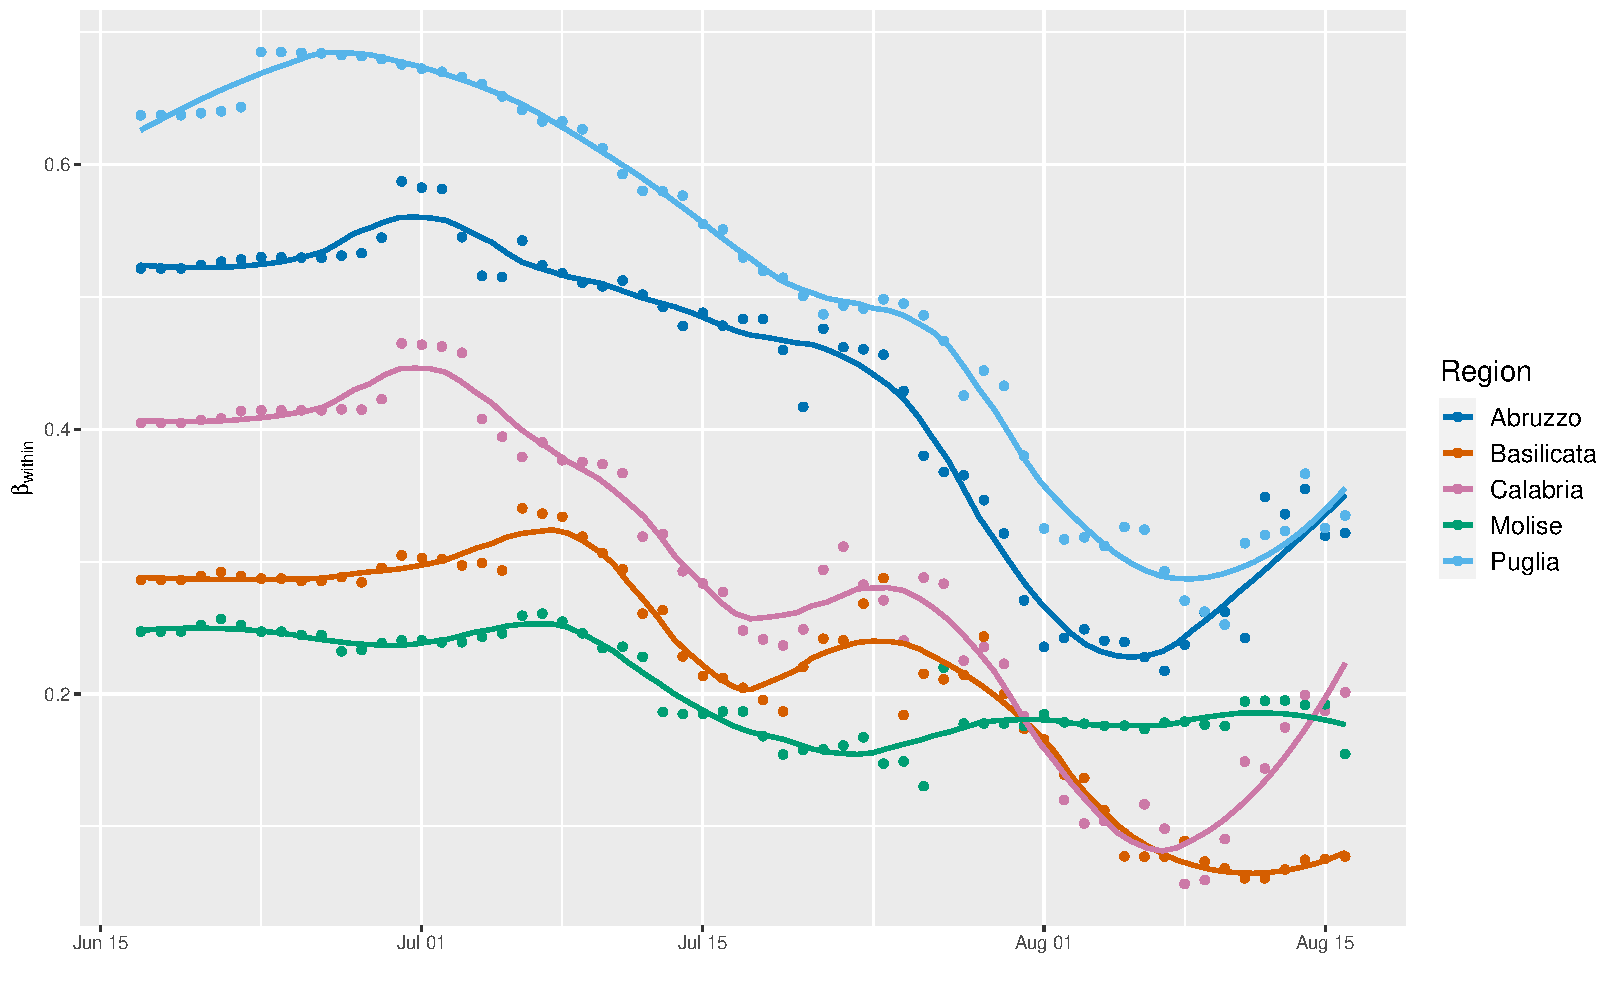
\includegraphics[width=0.92\linewidth]{output/model_within_lag14_betawithin_Sud_aic_UndocQuadratic_rolling.pdf}
    	      \caption{With model selection by AIC; \\ including undocumented infectives}
    	      \label{fig:beta_within_over_time_sud_aic_undoc}
    	    \end{subfigure}
    	    \caption{Progression of $\beta_{within}$ over time for the Sud NUTS 1 region. Data spans May 9 until August 16, 2020 (100 days). Undocumented infectives are modelled using the quadratic specification with $\gamma = 0.7$ and $f^{min}=0.1$.}
    	    \label{fig:beta_within_over_time_sud}
	    \end{figure}
		
		\begin{figure}[H]
    	    \centering
    	    \begin{subfigure}{\textwidth}
    	      \centering
    	      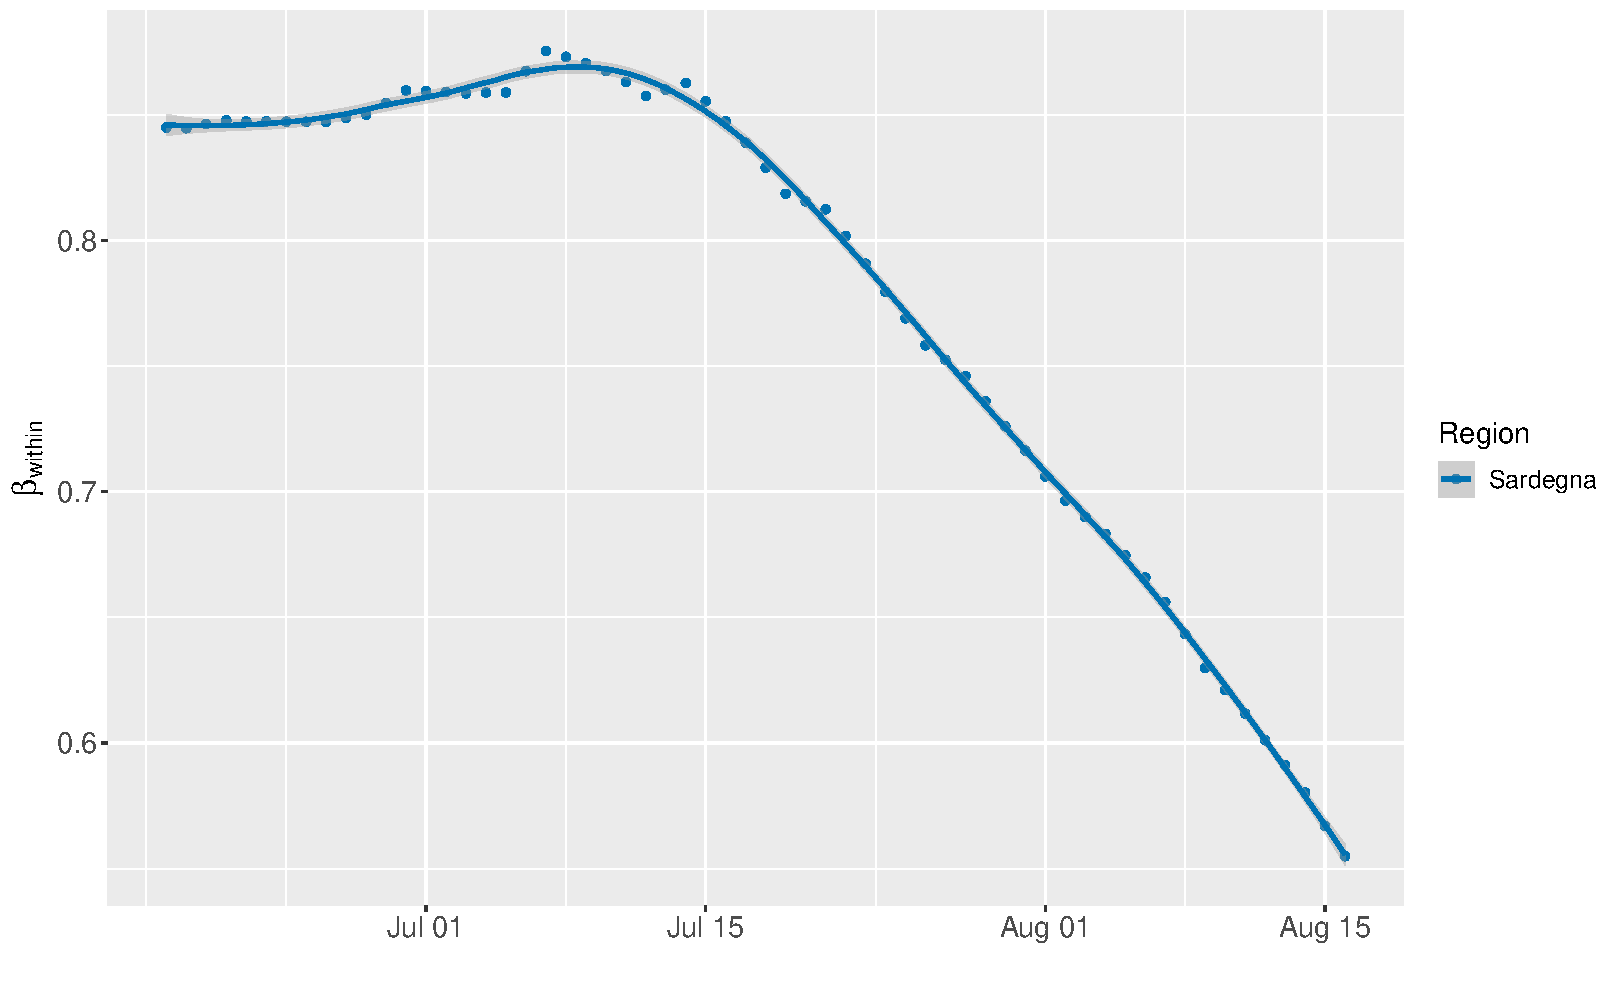
\includegraphics[width=0.92\linewidth]{output/model_within_lag14_betawithin_Isole_rolling.pdf}
    	      \caption{Without model selection}
    	      \label{fig:beta_within_over_time_isole_regular}
    	    \end{subfigure}\newline
    	    \begin{subfigure}{\textwidth}
    	      \centering
    	      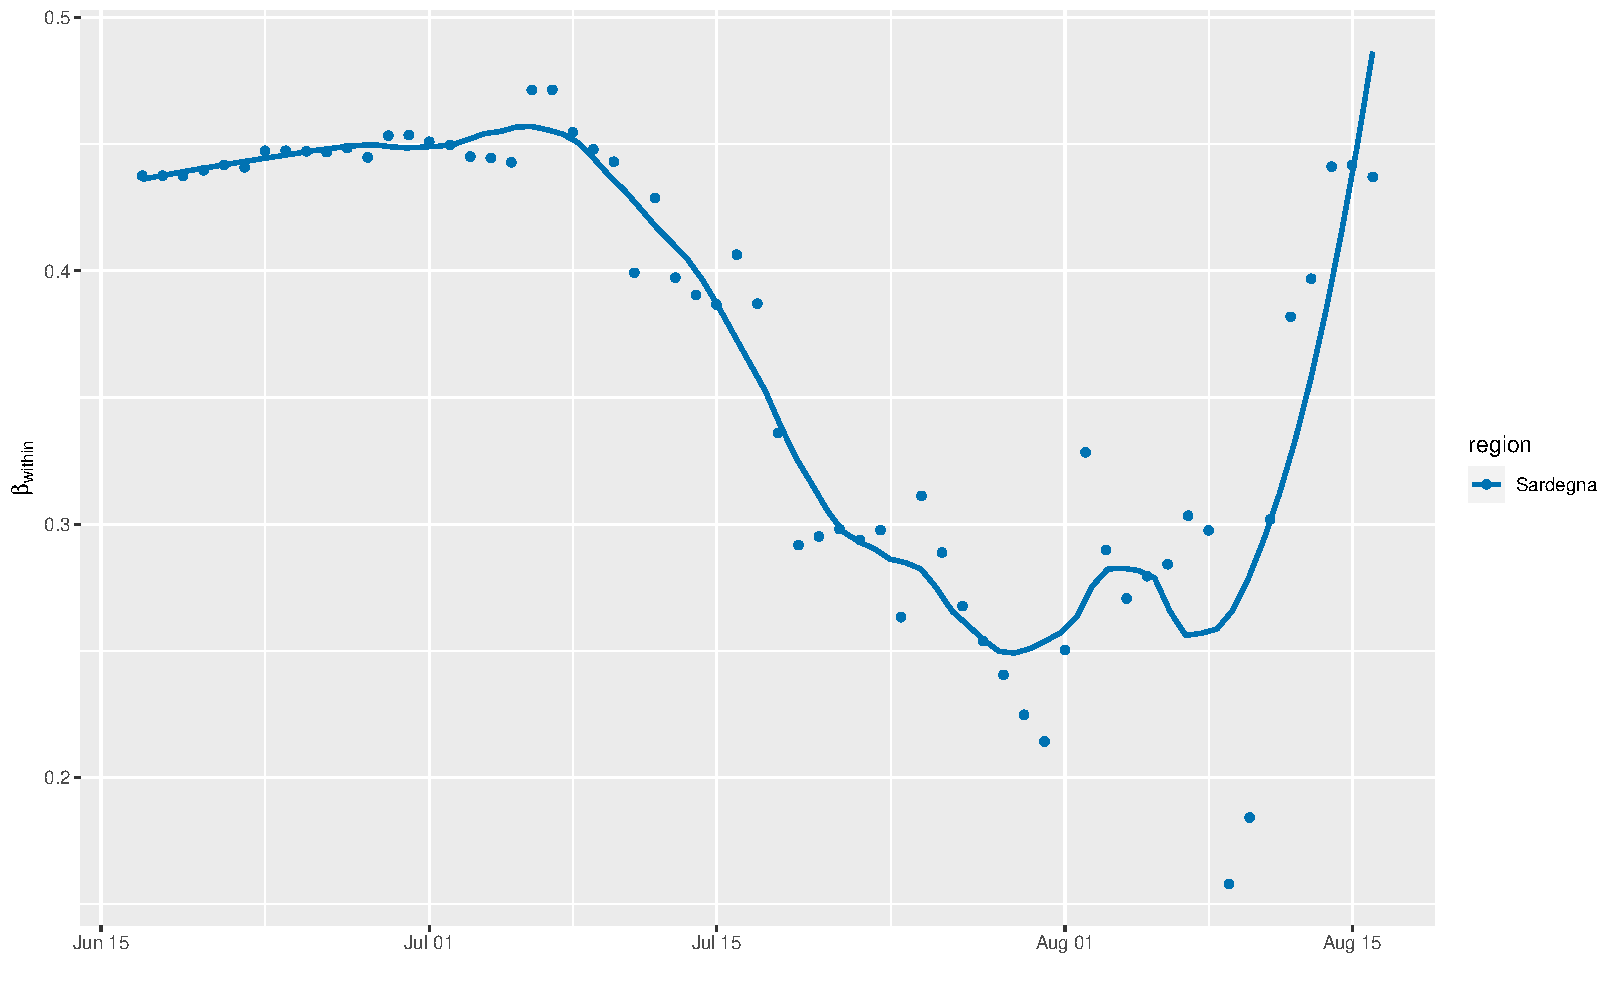
\includegraphics[width=0.92\linewidth]{output/model_within_lag14_betawithin_Isole_aic_rolling.pdf}
    	      \caption{With model selection by AIC}
    	      \label{fig:beta_within_over_time_isole_aic}
    	    \end{subfigure}
    	\end{figure}
        \begin{figure}[H]\ContinuedFloat
    	    \begin{subfigure}{\textwidth}
    	      \centering
    	      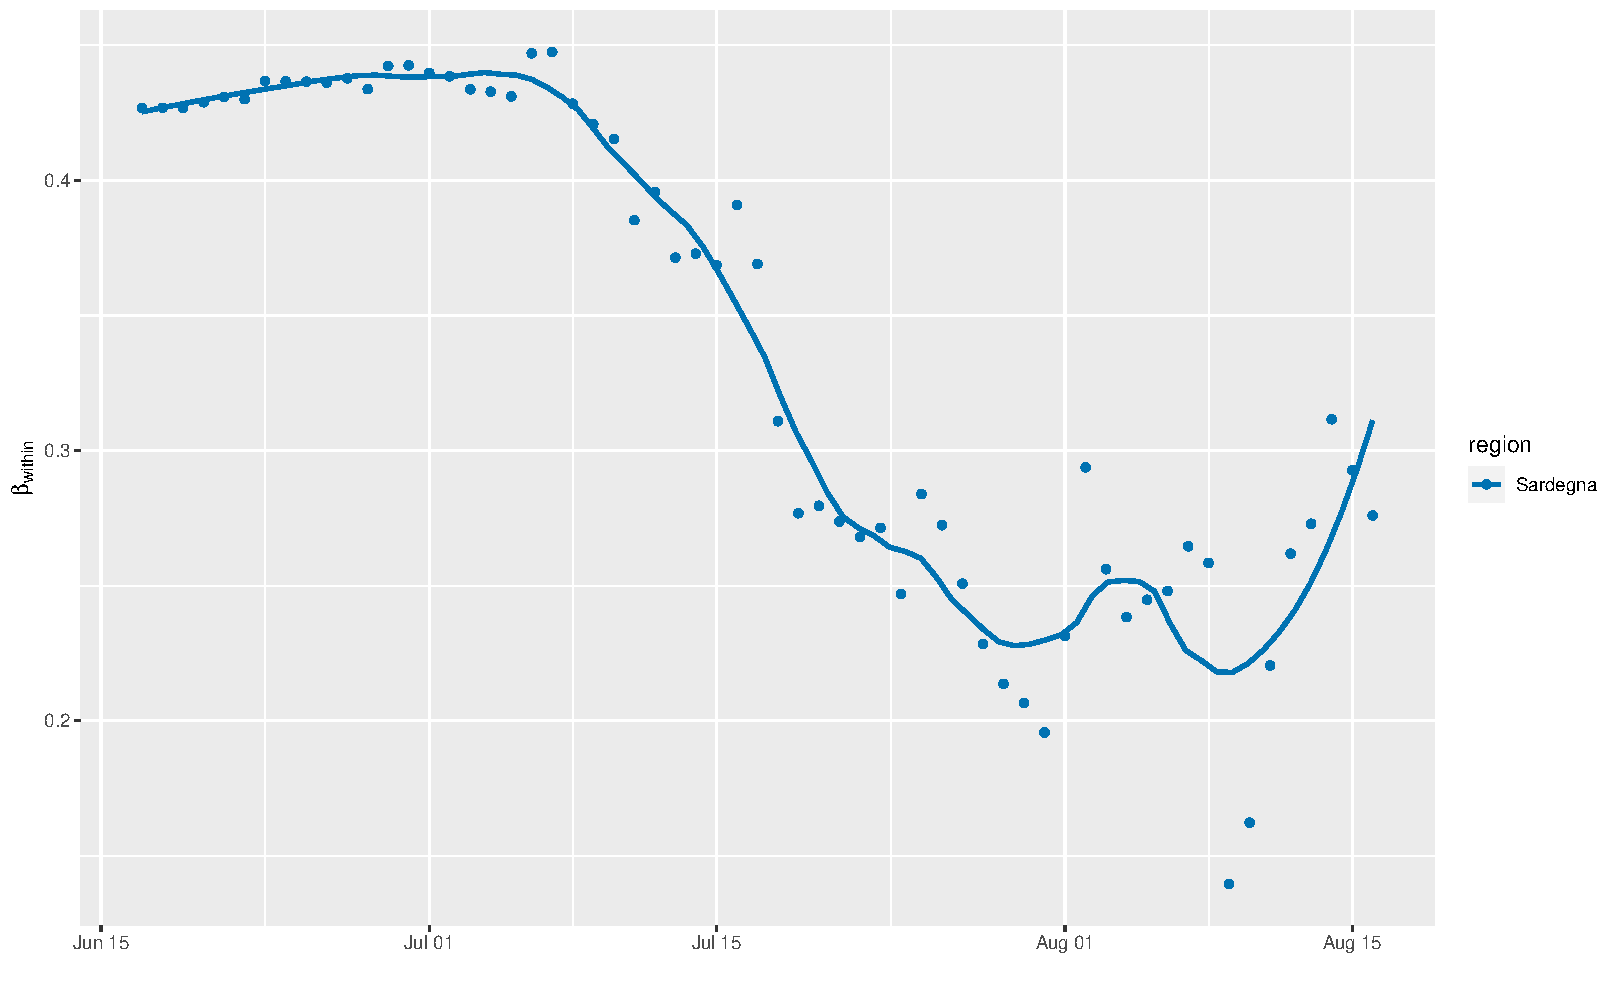
\includegraphics[width=0.92\linewidth]{output/model_within_lag14_betawithin_Isole_UndocQuadratic_rolling.pdf}
    	      \caption{Without model selection; \\ including undocumented infectives}
    	      \label{fig:beta_within_over_time_isole_regular_undoc}
    	    \end{subfigure}\newline
    	    \begin{subfigure}{\textwidth}
    	      \centering
    	      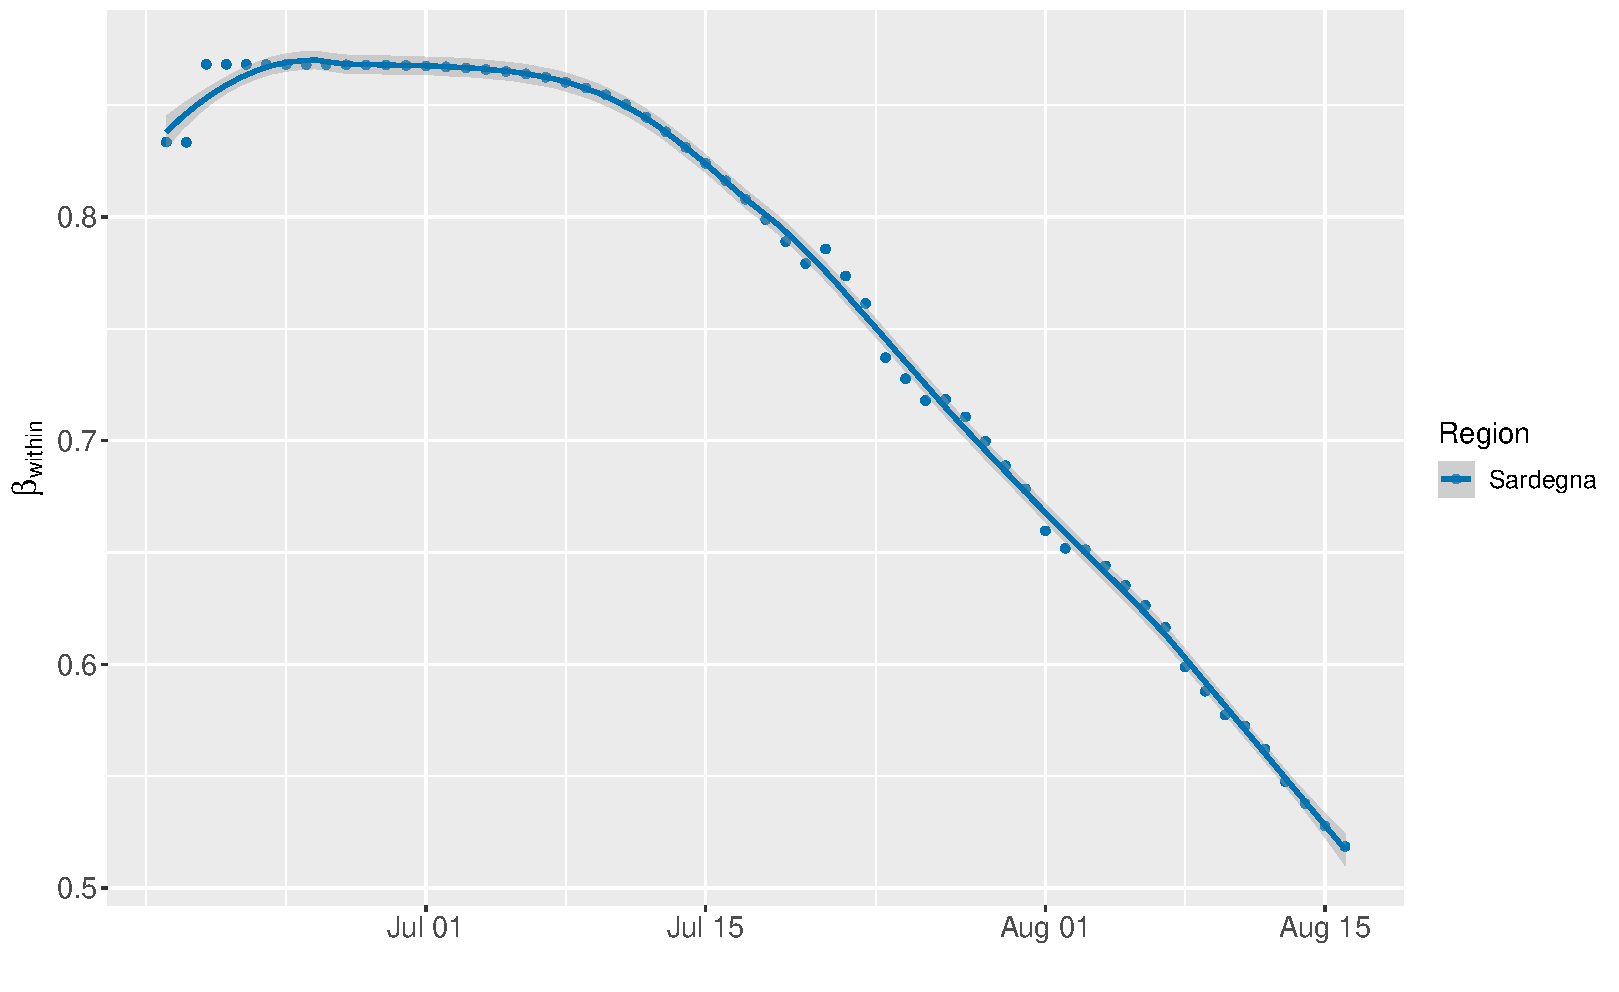
\includegraphics[width=0.92\linewidth]{output/model_within_lag14_betawithin_Isole_aic_UndocQuadratic_rolling.pdf}
    	      \caption{With model selection by AIC; \\ including undocumented infectives}
    	      \label{fig:beta_within_over_time_isole_aic_undoc}
    	    \end{subfigure}
    	    \caption{Progression of $\beta_{within}$ over time for the Isole NUTS 1 region. Data spans May 9 until August 16, 2020 (100 days). Undocumented infectives are modelled using the quadratic specification with $\gamma = 0.7$ and $f^{min}=0.1$.}
    	    \label{fig:beta_within_over_time_isole}
	    \end{figure}
		
		\subsection{Figures for the Within and Between-Region Spread Model} \label{sapp:model_between_figures}
		In Section \ref{subsec:model_between_results} we presented the plots of $\beta_{within}$ and $\beta_{between}$ over time for the Nord-Est NUTS 1 region for the within and between-region spread model. In this appendix, we present the plots for the other NUTS 1 regions.
		
		\begin{figure}[H]
    	    \centering
    	    \begin{subfigure}{\textwidth}
    	      \centering
    	      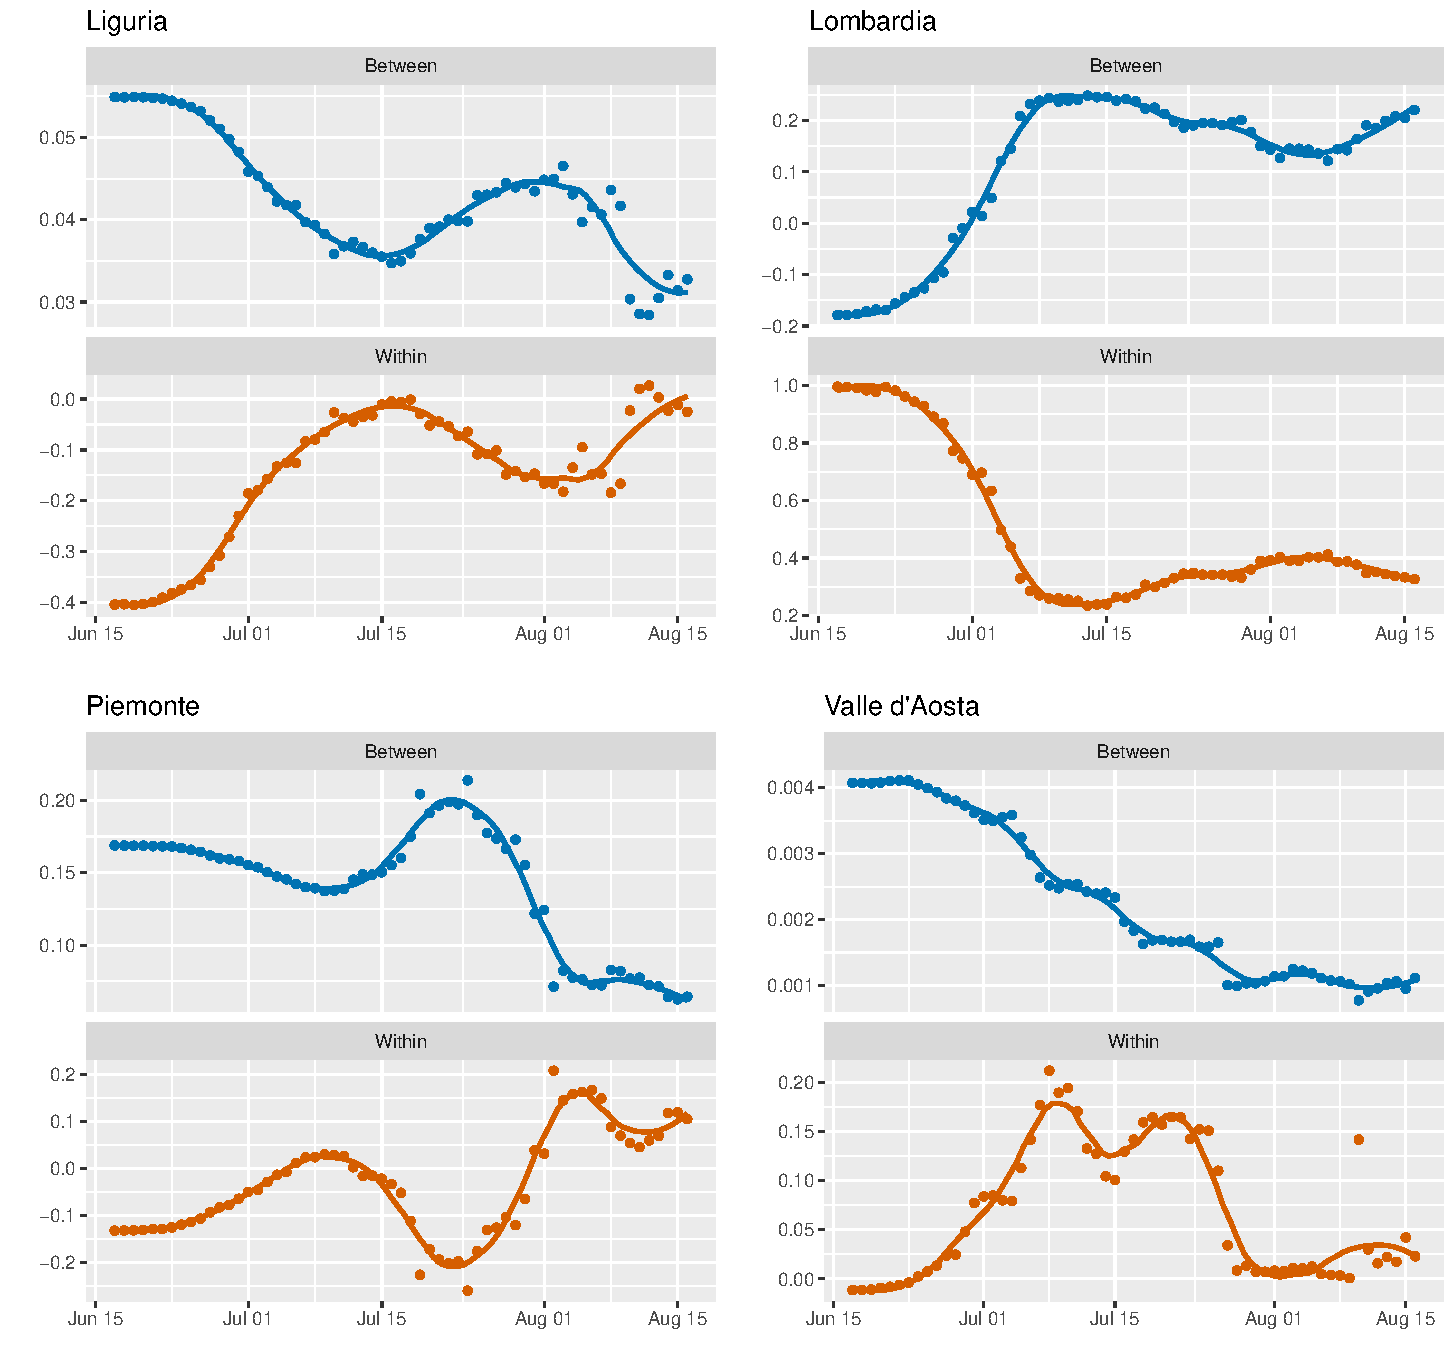
\includegraphics[width=\linewidth]{output/model_between_lag14_betas_Nord-Ovest_rolling.pdf}
    	      \caption{Without model selection}
    	      \label{fig:beta_between_over_time_nordovest_regular}
    	    \end{subfigure}
        \end{figure}
        \begin{figure}[H]\ContinuedFloat
    	    \begin{subfigure}{\textwidth}
    	      \centering
    	      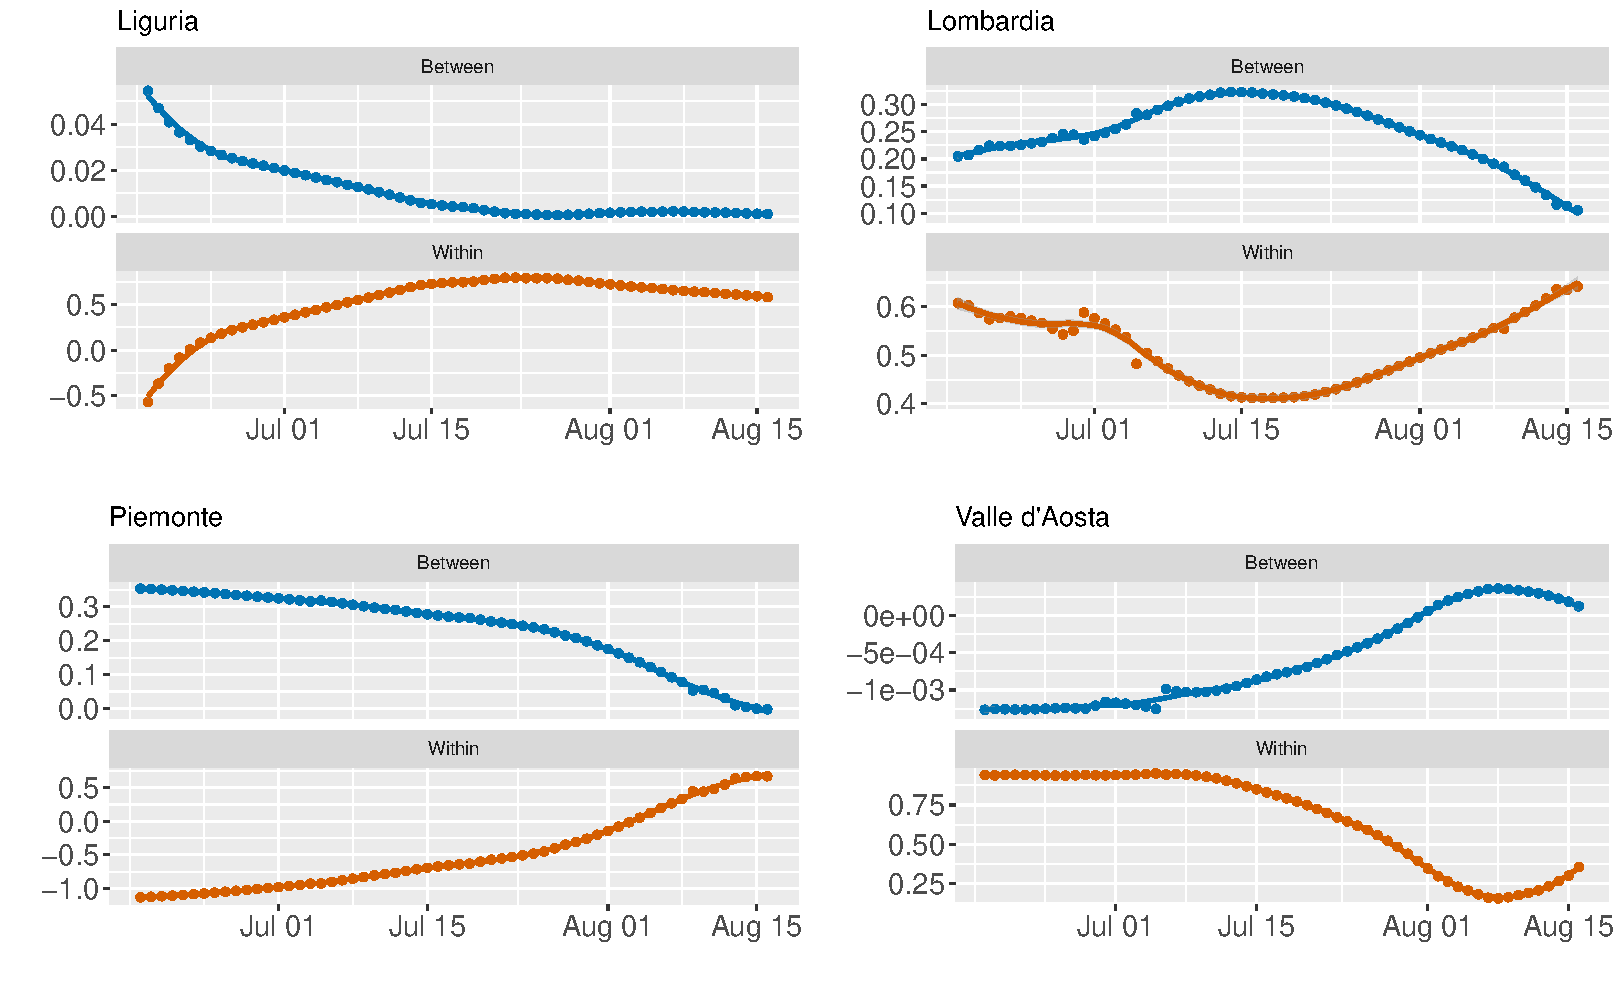
\includegraphics[width=\linewidth]{output/model_between_lag14_betas_Nord-Ovest_aic_rolling.pdf}
    	      \caption{With model selection by AIC}
    	      \label{fig:beta_between_over_time_nordovest_aic}
    	    \end{subfigure}
    	\end{figure}
        \begin{figure}[H]\ContinuedFloat
    	    \begin{subfigure}{\textwidth}
    	      \centering
    	      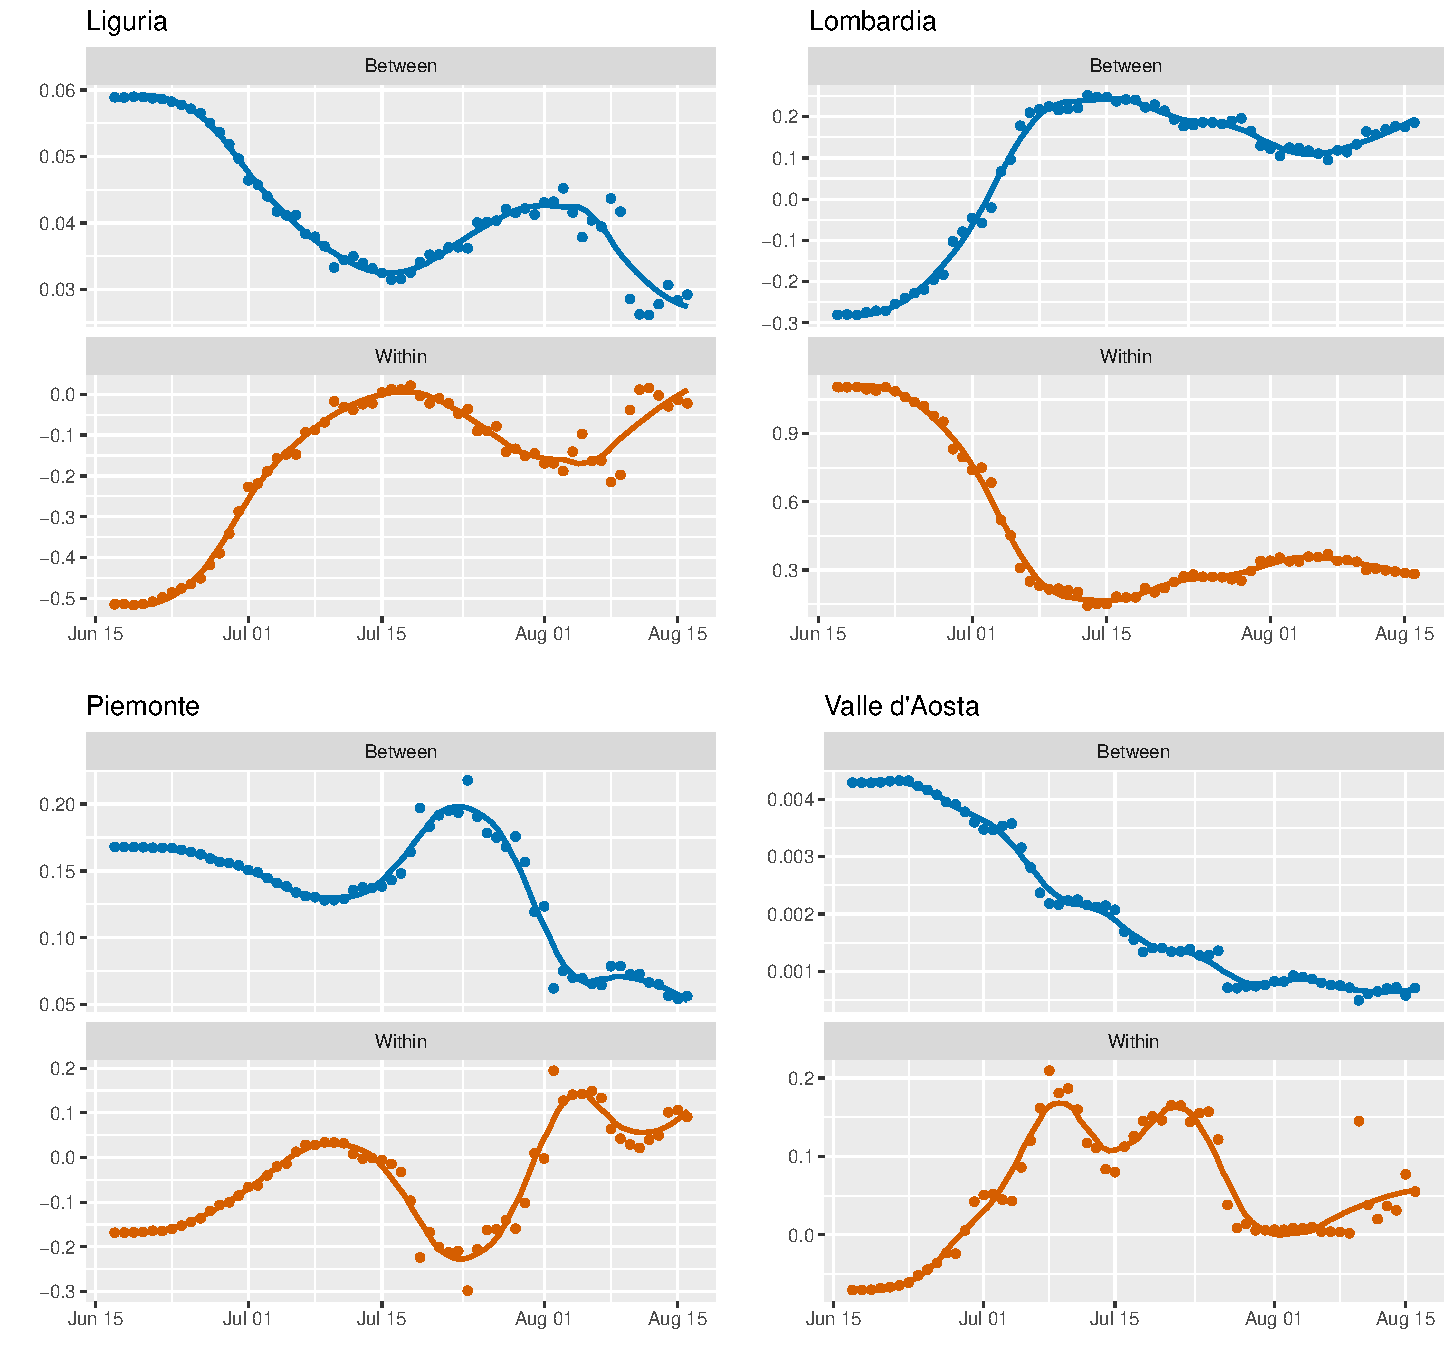
\includegraphics[width=\linewidth]{output/model_between_lag14_betas_Nord-Ovest_UndocQuadratic_rolling.pdf}
    	      \caption{Without model selection; \\ including undocumented infectives}
    	      \label{fig:beta_between_over_time_nordovest_regular_undoc}
    	    \end{subfigure}
        \end{figure}
        \begin{figure}[H]\ContinuedFloat
    	    \begin{subfigure}{\textwidth}
    	      \centering
    	      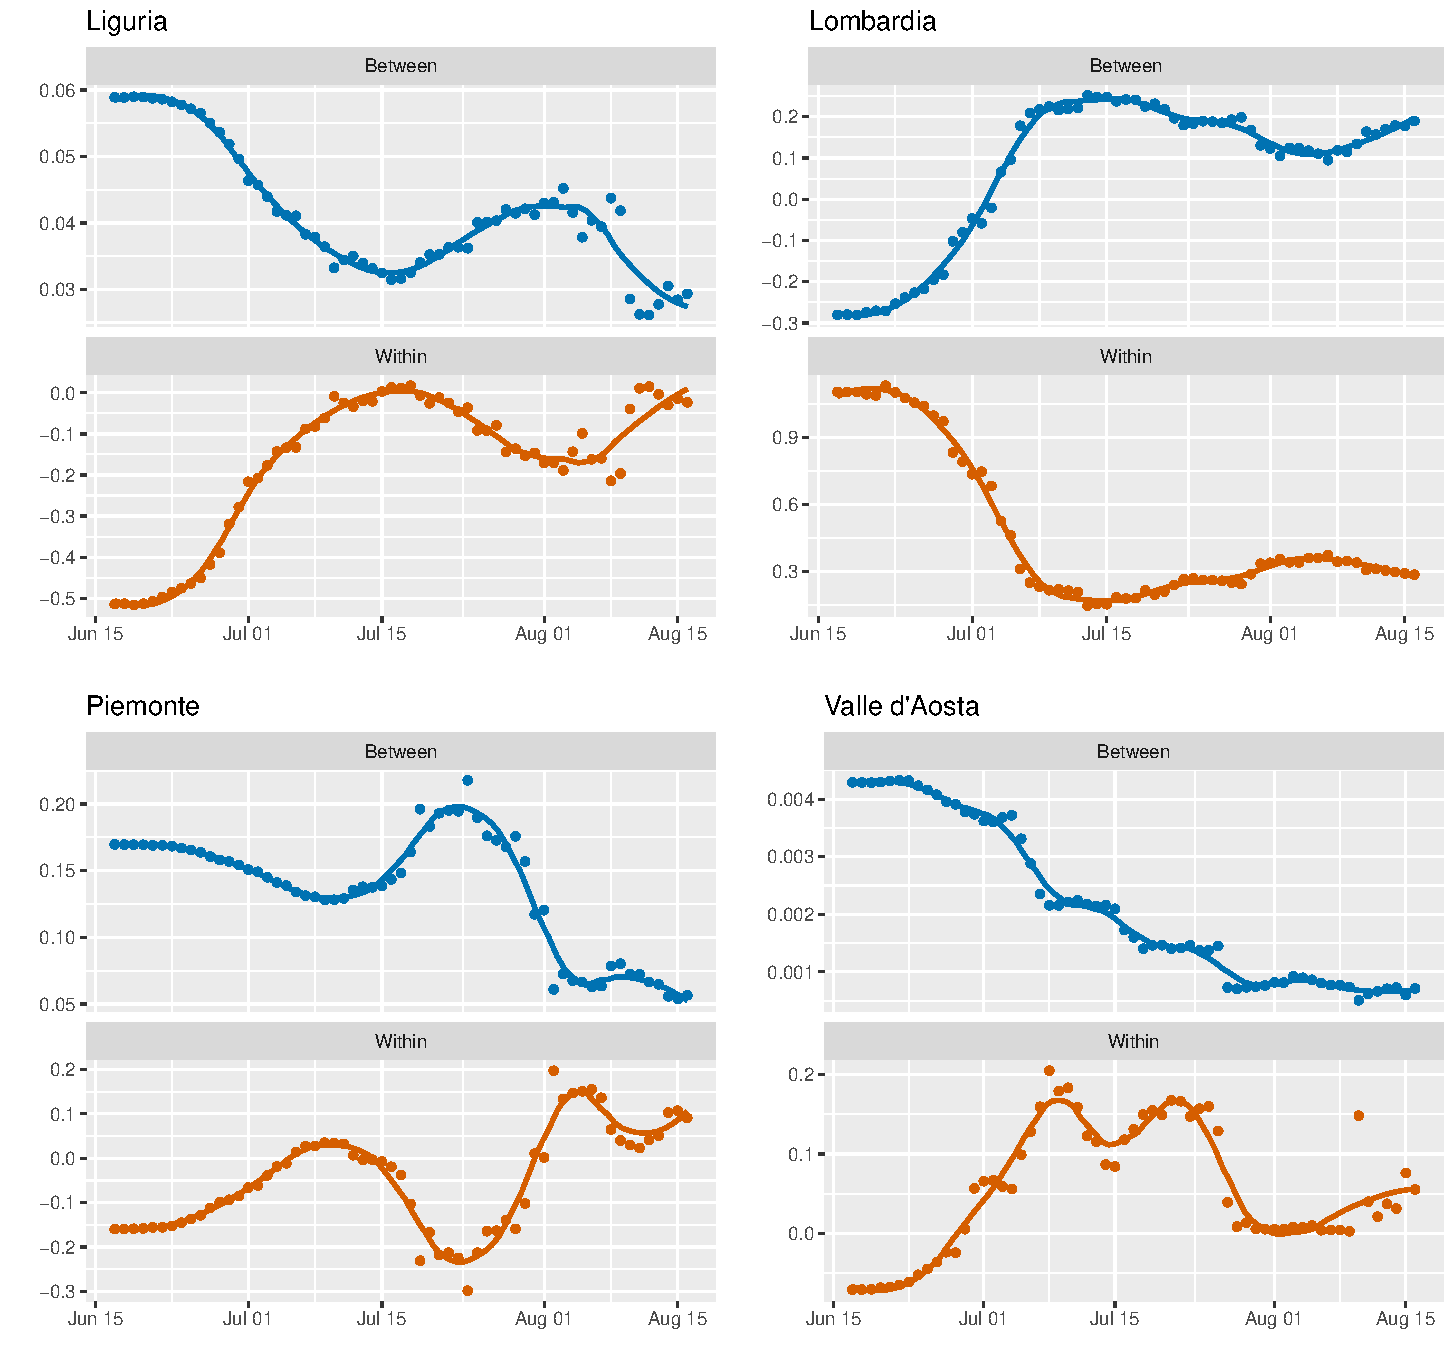
\includegraphics[width=\linewidth]{output/model_between_lag14_betas_Nord-Ovest_aic_UndocQuadratic_rolling.pdf}
    	      \caption{With model selection by AIC; \\ including undocumented infectives}
    	      \label{fig:beta_between_over_time_nordovest_aic_undoc}
    	    \end{subfigure}
    	    \caption{Progression of $\beta_{within}$ and $\beta_{between}$ over time for the Nord-Ovest NUTS 1 region. Data spans May 9 until August 16, 2020 (100 days). Undocumented infectives are modelled using the quadratic specification with $\gamma = 0.7$ and $f^{min}=0.1$.}
    	    \label{fig:beta_between_over_time_nordovest}
        \end{figure}
		
		\begin{figure}[H]
    	    \centering
    	    \begin{subfigure}{\textwidth}
    	      \centering
    	      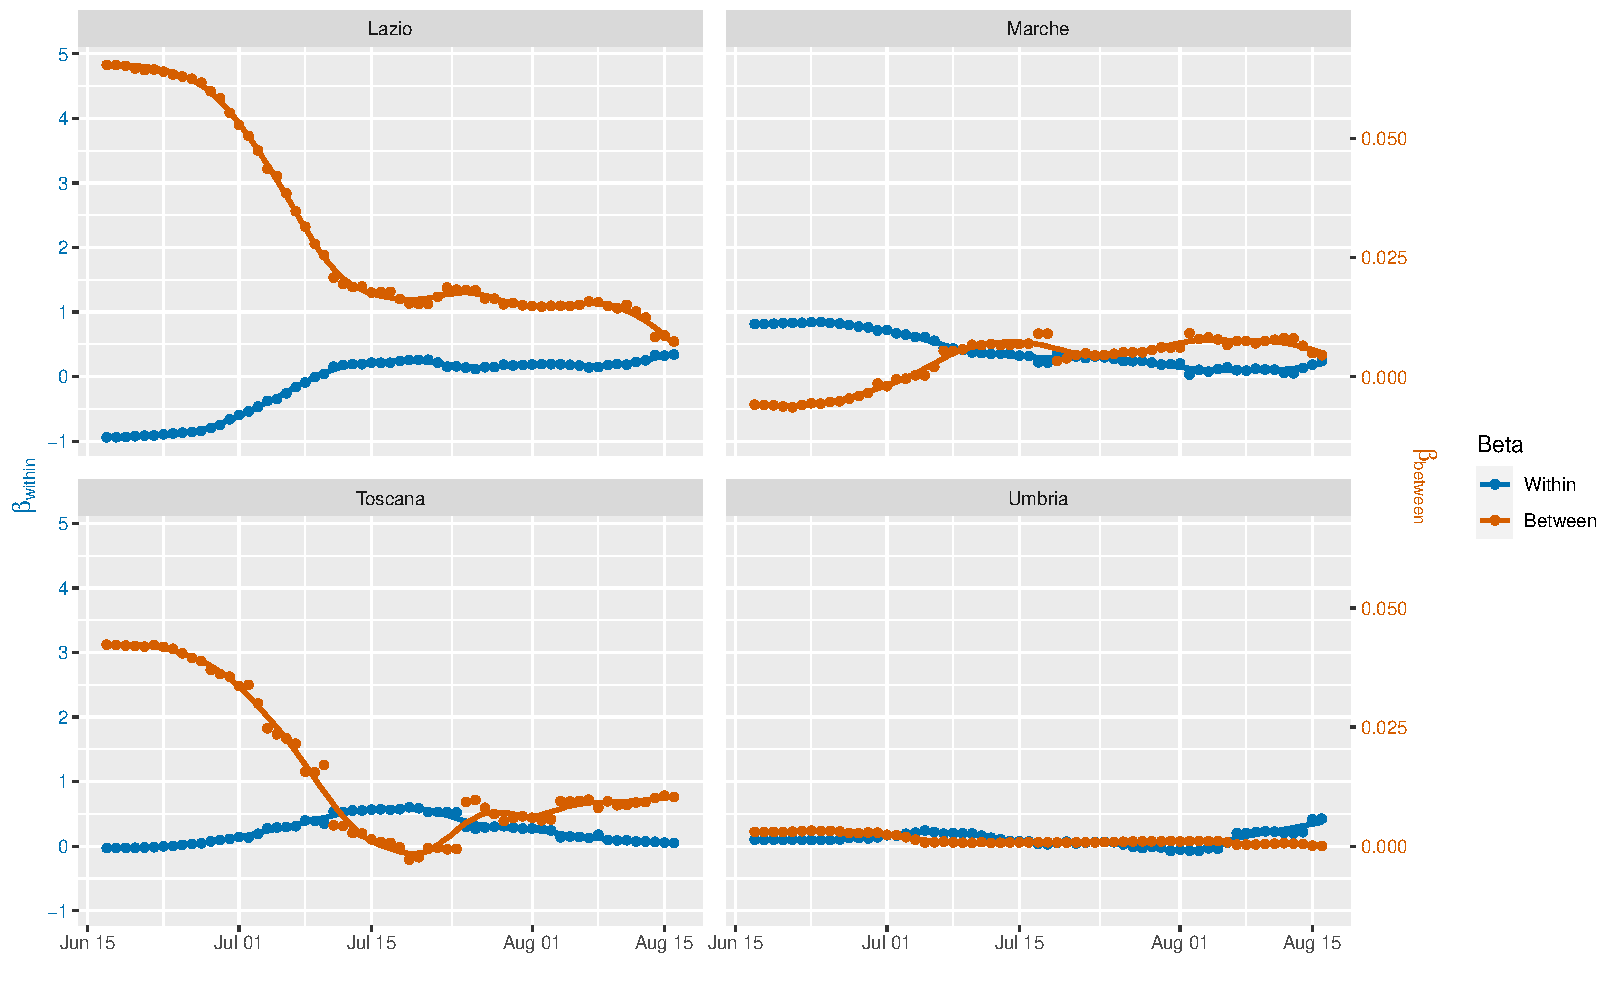
\includegraphics[width=\linewidth]{output/model_between_lag14_betas_Centro (IT)_rolling.pdf}
    	      \caption{Without model selection}
    	      \label{fig:beta_between_over_time_centro_regular}
    	    \end{subfigure}
        \end{figure}
        \begin{figure}[H]\ContinuedFloat
    	    \begin{subfigure}{\textwidth}
    	      \centering
    	      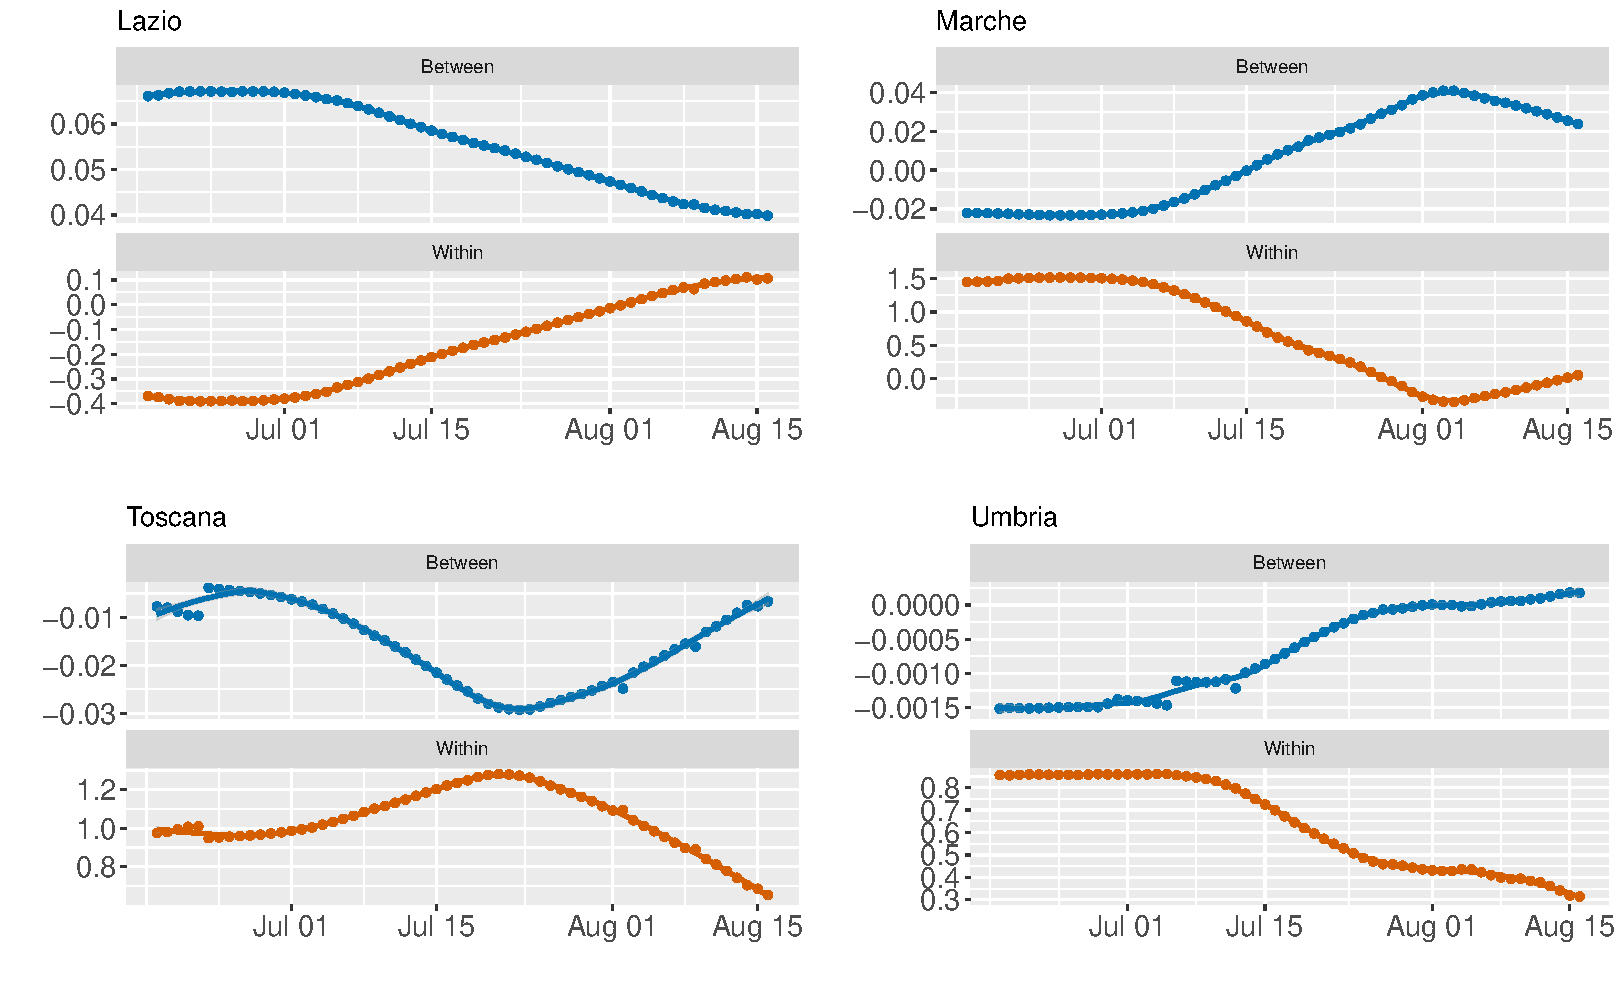
\includegraphics[width=\linewidth]{output/model_between_lag14_betas_Centro (IT)_aic_rolling.pdf}
    	      \caption{With model selection by AIC}
    	      \label{fig:beta_between_over_time_centro_aic}
    	    \end{subfigure}
    	\end{figure}
        \begin{figure}[H]\ContinuedFloat
    	    \begin{subfigure}{\textwidth}
    	      \centering
    	      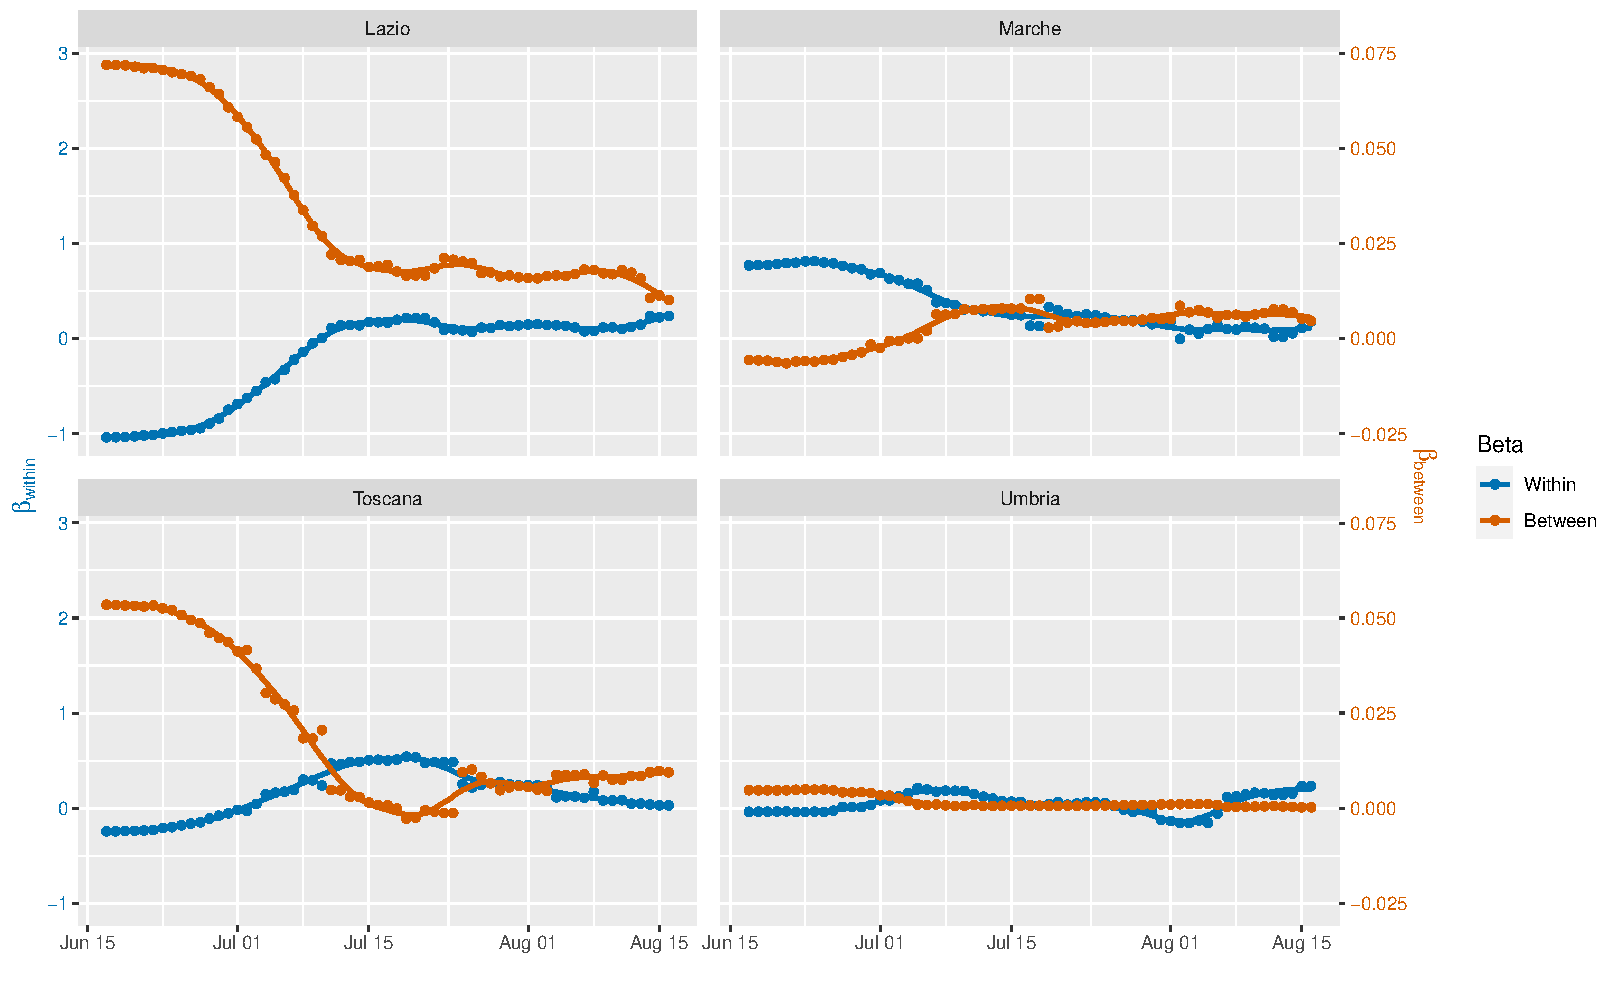
\includegraphics[width=\linewidth]{output/model_between_lag14_betas_Centro (IT)_UndocQuadratic_rolling.pdf}
    	      \caption{Without model selection; \\ including undocumented infectives}
    	      \label{fig:beta_between_over_time_centro_regular_undoc}
    	    \end{subfigure}
        \end{figure}
        \begin{figure}[H]\ContinuedFloat
    	    \begin{subfigure}{\textwidth}
    	      \centering
    	      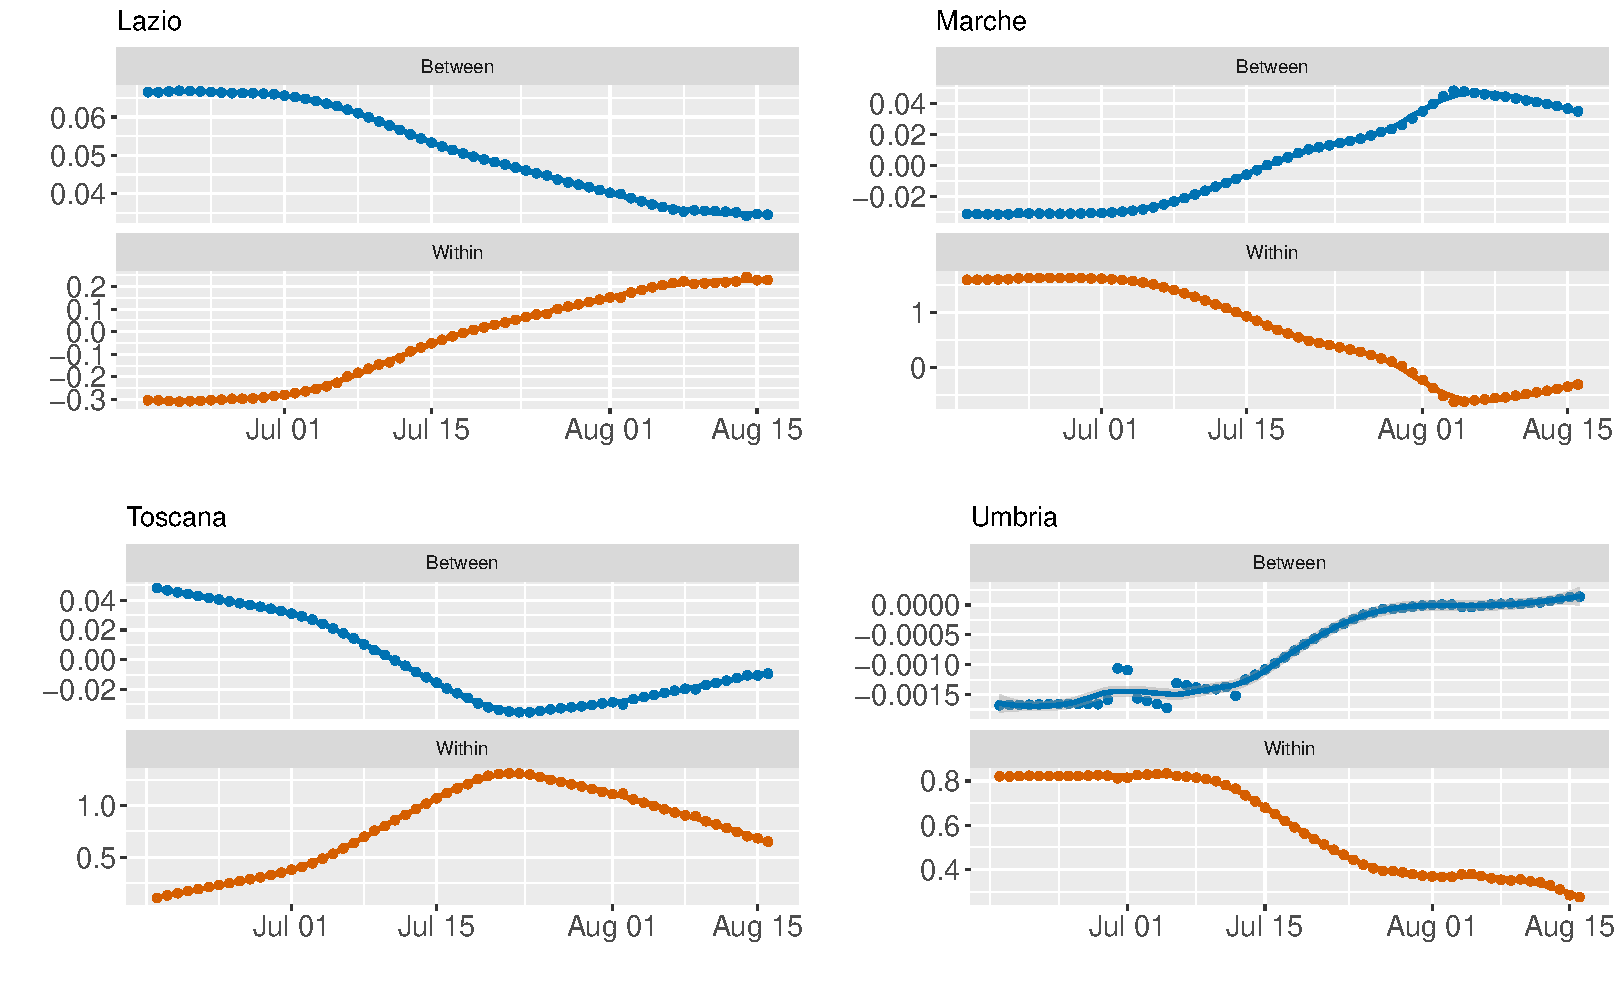
\includegraphics[width=\linewidth]{output/model_between_lag14_betas_Centro (IT)_aic_UndocQuadratic_rolling.pdf}
    	      \caption{With model selection by AIC; \\ including undocumented infectives}
    	      \label{fig:beta_between_over_time_centro_aic_undoc}
    	    \end{subfigure}
    	    \caption{Progression of $\beta_{within}$ and $\beta_{between}$ over time for the Centro (IT) NUTS 1 region. Data spans May 9 until August 16, 2020 (100 days). Undocumented infectives are modelled using the quadratic specification with $\gamma = 0.7$ and $f^{min}=0.1$.}
    	    \label{fig:beta_between_over_time_centro}
        \end{figure}
		
		\begin{figure}[H]
    	    \centering
    	    \begin{subfigure}{\textwidth}
    	      \centering
    	      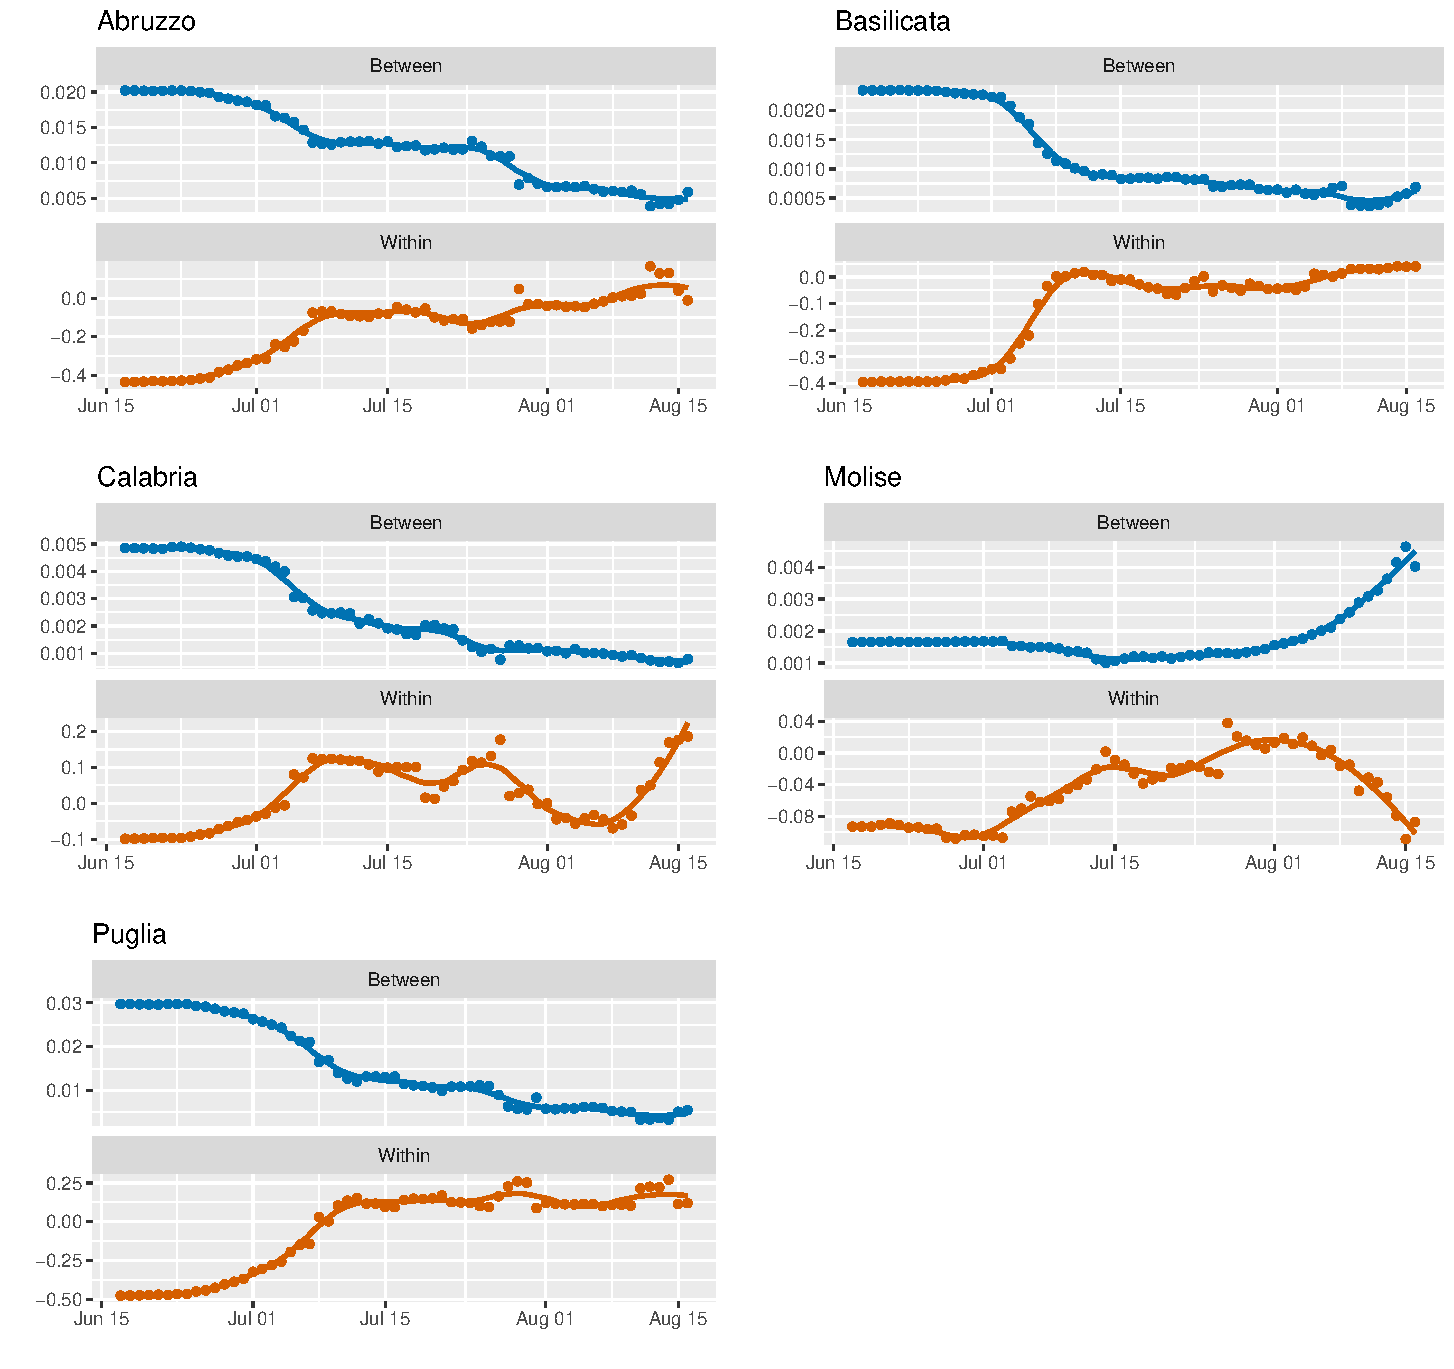
\includegraphics[width=\linewidth]{output/model_between_lag14_betas_Sud_rolling.pdf}
    	      \caption{Without model selection}
    	      \label{fig:beta_between_over_time_sud_regular}
    	    \end{subfigure}
        \end{figure}
        \begin{figure}[H]\ContinuedFloat
    	    \begin{subfigure}{\textwidth}
    	      \centering
    	      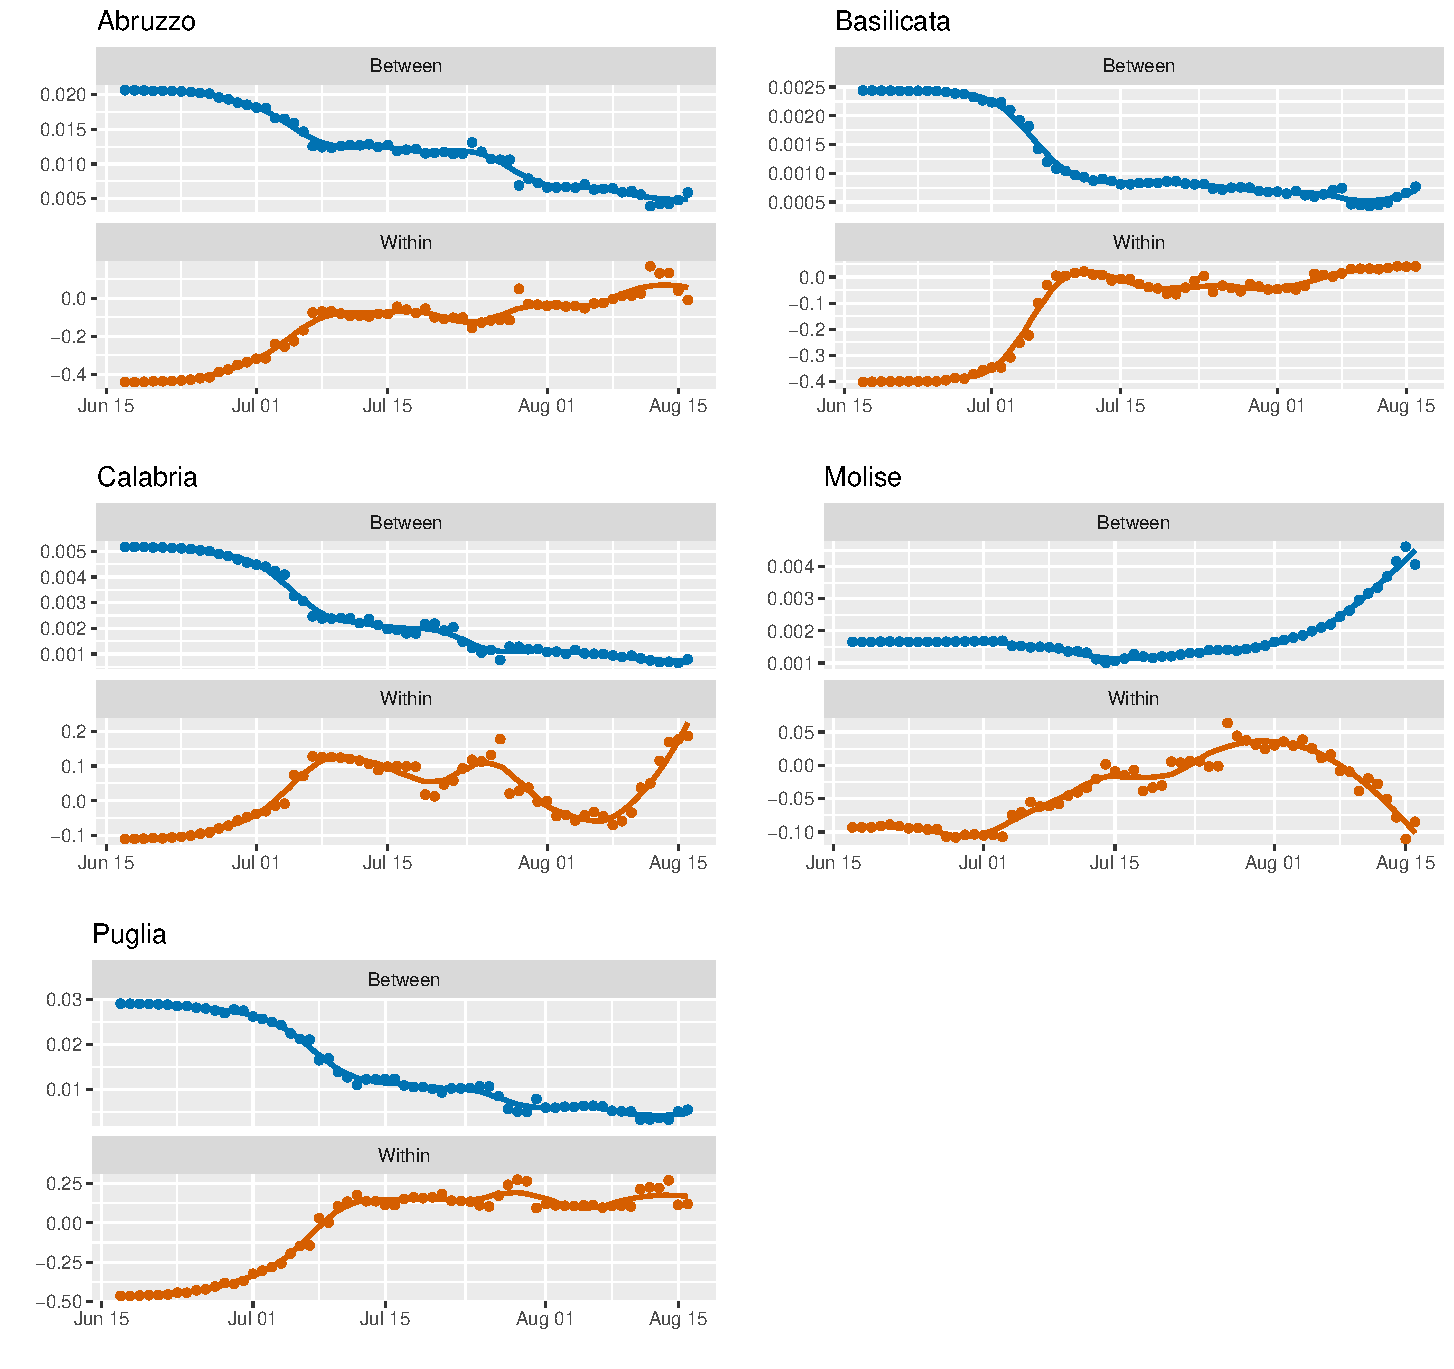
\includegraphics[width=\linewidth]{output/model_between_lag14_betas_Sud_aic_rolling.pdf}
    	      \caption{With model selection by AIC}
    	      \label{fig:beta_between_over_time_sud_aic}
    	    \end{subfigure}
    	\end{figure}
        \begin{figure}[H]\ContinuedFloat
    	    \begin{subfigure}{\textwidth}
    	      \centering
    	      \includegraphics[width=\linewidth]{output/model_between_lag14_betas_Sud_UndocQuadratic_rolling.pdf}
    	      \caption{Without model selection; \\ including undocumented infectives}
    	      \label{fig:beta_between_over_time_sud_regular_undoc}
    	    \end{subfigure}
        \end{figure}
        \begin{figure}[H]\ContinuedFloat
    	    \begin{subfigure}{\textwidth}
    	      \centering
    	      \includegraphics[width=\linewidth]{output/model_between_lag14_betas_Sud_aic_UndocQuadratic_rolling.pdf}
    	      \caption{With model selection by AIC; \\ including undocumented infectives}
    	      \label{fig:beta_between_over_time_sud_aic_undoc}
    	    \end{subfigure}
    	    \caption{Progression of $\beta_{within}$ and $\beta_{between}$ over time for the Sud NUTS 1 region. Data spans May 9 until August 16, 2020 (100 days). Undocumented infectives are modelled using the quadratic specification with $\gamma = 0.7$ and $f^{min}=0.1$.}
    	    \label{fig:beta_between_over_time_sud}
        \end{figure}
		
		\begin{figure}[H]
    	    \centering
    	    \begin{subfigure}{\textwidth}
    	      \centering
    	      \includegraphics[width=0.8\linewidth]{output/model_between_lag14_betas_Isole_rolling.pdf}
    	      \caption{Without model selection}
    	      \label{fig:beta_between_over_time_isole_regular}
    	    \end{subfigure}
        \end{figure}
        \begin{figure}[H]\ContinuedFloat
    	    \begin{subfigure}{\textwidth}
    	      \centering
    	      \includegraphics[width=0.8\linewidth]{output/model_between_lag14_betas_Isole_aic_rolling.pdf}
    	      \caption{With model selection by AIC}
    	      \label{fig:beta_between_over_time_isole_aic}
    	    \end{subfigure}
    	\end{figure}
        \begin{figure}[H]\ContinuedFloat
    	    \begin{subfigure}{\textwidth}
    	      \centering
    	      \includegraphics[width=0.8\linewidth]{output/model_between_lag14_betas_Isole_UndocQuadratic_rolling.pdf}
    	      \caption{Without model selection; \\ including undocumented infectives}
    	      \label{fig:beta_between_over_time_isole_regular_undoc}
    	    \end{subfigure}
        \end{figure}
        \begin{figure}[H]\ContinuedFloat
    	    \begin{subfigure}{\textwidth}
    	      \centering
    	      \includegraphics[width=0.8\linewidth]{output/model_between_lag14_betas_Isole_aic_UndocQuadratic_rolling.pdf}
    	      \caption{With model selection by AIC; \\ including undocumented infectives}
    	      \label{fig:beta_between_over_time_isole_aic_undoc}
    	    \end{subfigure}
    	    \caption{Progression of $\beta_{within}$ and $\beta_{between}$ over time for the Isole NUTS 1 region. Data spans May 9 until August 16, 2020 (100 days). Undocumented infectives are modelled using the quadratic specification with $\gamma = 0.7$ and $f^{min}=0.1$.}
    	    \label{fig:beta_between_over_time_isole}
        \end{figure}
		
		\newpage
		\section{Discrete SIR Model} \label{app:discrete_SIR}
		In Section \ref{sec:future_research}, we referenced an approach that aimed to discretize the SIR model to allow for the estimation of both the transmission rate and recovery rate, with the goal of obtaining an estimate of the effective reproduction number. Especially, the approach aimed to take into account the spatiotemporal nature of the data by applying panel data estimation techniques. In this appendix, we highlight the most important parts of this method, focusing on the methodology and presenting some results.
		
		\subsection{Methodology} \label{sapp:discrete_SIR_methodology}
		In this appendix, we discuss the methodology behind the discretized SIR model. Starting from the equations in Section \ref{sec:sir_model}, we acknowledge the addition by \textcite{adda2016economic} of a longer lag to take the incubation period into account. This leads to the following discretized equations:
		
		\begin{align}
        	S_{p,t} - S_{p,t-1} &= -\beta S_{p,t-\tau}I_{p,t-\tau} + \eta_{p,t}, \label{eq:discrete_SIR_model_S}\\
        	I_{p,t} - I_{p,t-1} &= \beta S_{p,t-\tau}I_{p,t-\tau} - \gamma I_{p,t-1} + \eta_{p,t}, \label{eq:discrete_SIR_model_I}\\
        	R_{p,t} - R_{p,t-1} &= \gamma I_{p,t-1} + \eta_{p,t}. \label{eq:discrete_SIR_model_R}
    	\end{align}
	
    	Two methods were explored to estimate the parameters. Firstly, we can apply estimation methods to \eqref{eq:discrete_SIR_model_S} and \eqref{eq:discrete_SIR_model_R} individually to obtain the estimates for $\beta$ and $\gamma$ individually. We would call this the regular model. The second method would be to first estimate one of the parameters by means of \eqref{eq:discrete_SIR_model_R} \eqref{eq:discrete_SIR_model_S} and then to we would fill in this estimate in \eqref{eq:discrete_SIR_model_I} to estimate the remaining parameter. If we use equation \ref{eq:discrete_SIR_model_I} to estimate $\gamma$ and use the resulting estimate $\hat{\gamma}$ in \eqref{eq:discrete_SIR_model_I} to obtain:
    	    
    	    \begin{equation} \label{eq:discrete_SIR_model_I_twostep}
    	        \begin{split}
            		& I_{p,t} - I_{p,t-1} = \beta S_{p,t-\tau}I_{p,t-\tau} - \hat{\gamma} I_{p,t-1} + \eta_{p,t} \\
        	        \iff & I_{p,t} - \left(1 - \hat{\gamma}\right) I_{p,t-1} = \beta S_{p,t-\tau}I_{p,t-\tau} + \eta_{p,t}.
        		\end{split}
    	    \end{equation}
	
	    There are three main panel data models that are usually applied: the pooled OLS (POLS), fixed effects (FE), and random effects (RE) models. The choice between these models depends on the assumptions that are placed on the individual effect $\alpha_i$. The fixed effects model, in essence, assumes that each individual (region) has a time-constant intercept. The SIR model, on the other hand, does not include an intercept in its formulation. The reason behind this is intuitive: there is not some non-zero mean number of new cases that is persistent throughout time for a certain region. Because of this, the fixed effects model is not suitable for our estimation. \\
    	
    	The main idea behind the random effects model is to impose a distribution on the regional effects that can then be included in the error term: $\alpha_i \sim N\left(0, \sigma^2_{\alpha}\right)$. This assumption may indeed be in line with the SIR model because the mean heterogeneous effect is assumed to be zero. Lastly, the pooled OLS model ignores the regional effect, hence treating the data as one large cross-section. This means that the $T$ observations for some region $p$ are actually treated to be cross-sectional observations of $T$ different individuals. We apply both random effects and pooled OLS and compare the results.
	
	    \subsection{Results} \label{sapp:discrete_sir_results}
		In this section, we present the results for the discretized SIR model. Table \ref{tab:results_discrete_panel_frequency_undoc} shows the results of estimating the parameters excluding and including undocumented infectives for two values of the lag $\tau$, namely $\tau = 1$ as in the original SIR model and $\tau = 14$ as in the models by \textcite{adda2016economic}. Note that the estimate of $\gamma$ is the same regardless of the choice of $\tau$. Recall that this is because $\gamma$ is estimated from equation \eqref{eq:discrete_SIR_model_R}, in which no lag other than 1 is used.
	
    	\begin{longtable}{@{}lcccccc@{}}
    		\caption{Estimates for the discretized SIR model with panel data methods. Estimates are given with $t$-statistics (for POLS) or $z$-statistics (for RE) in parentheses. Data spans May 9 until August 16, 2020 (100 days). Undocumented infectives are modelled using the quadratic specification with $\gamma = 0.7$ and $f^{min}=0.1$.}
    		\label{tab:results_discrete_panel_frequency_undoc}\\
    		\toprule
    		                && \multicolumn{2}{c}{Regular model} & \multicolumn{2}{c}{Modelling undocumented infectives} \\
    		                \cmidrule(lr){3-4}
                            \cmidrule(lr){5-6}
    		$\tau$          & Parameter & $POLS$ & $RE$ & $POLS$ & $RE$ \\* \midrule
    		\endfirsthead
    		
    		\multicolumn{6}{c}{{\bfseries Table \thetable\ continued from previous page}} \\
    		\toprule
    		                && \multicolumn{2}{c}{Regular model} & \multicolumn{2}{c}{Modelling undocumented infectives} \\
    		                \cmidrule(lr){3-4}
                            \cmidrule(lr){5-6}
    		$\tau$          & Parameter & $POLS$ & $RE$ & $POLS$ & $RE$ \\* \midrule
    		\endhead
    		
    		\bottomrule
    		\multicolumn{6}{c}{{\bfseries Table \thetable\ continues on next page}}
    		\endfoot
    		
    		\multicolumn{6}{c}{Significance levels: * = 0.1 ** = 0.05, *** = 0.01}
    		\endlastfoot
    		
    		& $\gamma$ & $4.886 \times 10^{-3}$*** & $4.425 \times 10^{-3}$*** & $6.187 \times 10^{-4}$*** & $5.888 \times 10^{-4}$*** \\ 
             &  & (26.859) & (13.888) & (27.537) & (15.606) \\
    		\midrule
            \multirow{4}{*}{1} & $\beta$ & $6.501 \times 10^{-3}$*** & $4.879 \times 10^{-3}$*** & $1.886 \times 10^{-3}$*** & $9.089 \times 10^{-6}$*** \\  
             &  & (30.680) & (9.310) & (29.100) & (0.029) \\ 
             & $\beta_{two\text{-}step}$ & $6.769 \times 10^{-3}$*** & $3.958 \times 10^{-3}$*** & $1.920 \times 10^{-3}$*** & $-1.198 \times 10^{-4}$*** \\ 
             &  & (107.921) & (14.120) & (36.995) & ($-0.420$) \\
             \cmidrule(lr){2-6}
             & $R_{eff}$ & 1.331 & 1.103 & 3.048 & 1.544 \\
             & $R_{eff;two\text{-}step}$ & 1.385 & 0.894 & 3.103 & $-0.203$ \\
            \midrule
            \multirow{4}{*}{14} & $\beta$ & $6.356 \times 10^{-3}$*** & $2.028 \times 10^{-3}$*** & $1.821 \times 10^{-3}$*** & $-3.641 \times 10^{-4}$*** \\  
             &  & (28.459) & (3.403) & (26.925) & ($-0.525$) \\ 
             & $\beta_{two\text{-}step}$ & $6.853 \times 10^{-3}$*** & $1.901 \times 10^{-5}$*** & $1.877 \times 10^{-3}$*** & $-3.358 \times 10^{-3}$*** \\ 
             &  & (96.760) & (0.060) & (34.469) & (-11.315) \\
             \cmidrule(lr){2-6}
             & $R_{eff}$ & 1.301 & 0.458 & 2.943 & $-0.618$ \\
             & $R_{eff;two\text{-}step}$ & 1.403 & $4.296 \times 10^{-3}$ & 3.034 & $-5.703$ \\* \bottomrule
    	\end{longtable}
    	
    	Table \ref{tab:results_discrete_panel_frequency_undoc} shows us that all estimates are statistically significant at a significance level of 0.01. Firstly, notice that the random effects model when including undocumented infectives yields negative estimates, which are not possible. As such, it is not applicable to this situation. This also becomes clear when considering the results on $R_{eff}$, which are too low for the random effects model. It is also interesting to compare the values of $R_{eff}$ when modelling undocumented infectives. Indeed, the effect that the values of $R_{eff}$ are larger when undocumented infectives are included is higher, is to be expected. \\
    	
    	Unfortunately, all estimates are quite low. Consider the estimate of $\gamma = 4.886 \times 10^{-3}$. This implies that the average infectious period is $\gamma^{-1} = 204.67$ days, which is not credible. Unfortunately, this means that the estimates are not individually interpretable. However, it may be possible that the resulting value of $R_{eff}$ is indeed correct if the estimates of $\beta$ and $\gamma$ both differ from their true value by the same factor. \\
		
		Figures \ref{fig:beta_over_time_panel_data_all}, \ref{fig:gamma_over_time_panel_data_all}, and \ref{fig:Reff_over_time_panel_data_all} show the progression of the transmission rate $\beta$, the recovery rate $\gamma$, and the effective reproduction number $R_{eff}$ over time, respectively. Each point in the graphs is the estimate of $\beta$, $\gamma$, or the resulting value of $R_{eff}$ when only the latest 100 data points before that date are used. In addition, a LOESS curve with span parameter 0.3 is fit to the data points.
		
		\begin{figure}[H]
    	    \centering
    	    \begin{subfigure}{0.495\textwidth}
    	      \centering
    	      \includegraphics[width=\linewidth]{output/panel_data_lag14_betas_rolling.pdf}
    	      \caption{Excluding undocumented infectives}
    	      \label{fig:beta_over_time_panel_data_rolling}
    	    \end{subfigure}
    	    \begin{subfigure}{0.495\textwidth}
    	      \centering
    	      \includegraphics[width=\linewidth]{output/panel_data_lag14_betas_UndocQuadratic_rolling.pdf}
    	      \caption{Including undocumented infectives}
    	      \label{fig:beta_over_time_panel_data_undoc_rolling}
    	    \end{subfigure}
    	    \caption{Progression of the transmission rate $\beta$ over time. Data spans May 9 until August 16, 2020 (100 days). Undocumented infectives are modelled using the quadratic specification with $\gamma = 0.7$ and $f^{min}=0.1$.}
    	    \label{fig:beta_over_time_panel_data_all}
    	\end{figure}
		
		\begin{figure}[H]
    	    \centering
    	    \begin{subfigure}{0.495\textwidth}
    	      \centering
    	      \includegraphics[width=\linewidth]{output/panel_data_lag14_gammas_rolling.pdf}
    	      \caption{Excluding undocumented infectives}
    	      \label{fig:gamma_over_time_panel_data}
    	    \end{subfigure}
    	    \begin{subfigure}{0.495\textwidth}
    	      \centering
    	      \includegraphics[width=\linewidth]{output/panel_data_lag14_gammas_UndocQuadratic_rolling.pdf}
    	      \caption{Including undocumented infectives}
    	      \label{fig:gamma_over_time_panel_data_undoc_rolling}
    	    \end{subfigure}
    	    \caption{Progression of the recovery rate $\gamma$ over time. With a rolling window, data spans May 9 until August 16, 2020 (100 days). Undocumented infectives are modelled using the quadratic specification with $\gamma = 0.7$ and $f^{min}=0.1$.}
    	    \label{fig:gamma_over_time_panel_data_all}
    	\end{figure}
		
		\begin{figure}[H]
    	    \centering
    	    \begin{subfigure}{0.495\textwidth}
    	      \centering
    	      \includegraphics[width=\linewidth]{output/panel_data_lag14_Reff_rolling.pdf}
    	      \caption{Excluding undocumented infectives}
    	      \label{fig:Reff_over_time_panel_data}
    	    \end{subfigure}
    	    \begin{subfigure}{0.495\textwidth}
    	      \centering
    	      \includegraphics[width=\linewidth]{output/panel_data_lag14_Reff_UndocQuadratic_rolling.pdf}
    	      \caption{Including undocumented infectives}
    	      \label{fig:Reff_over_time_panel_data_undoc_rolling}
    	    \end{subfigure}
    	    \caption{Progression of the effective reproduction number $R_{eff}$ over time. With a rolling window, data spans May 9 until August 16, 2020 (100 days). Undocumented infectives are modelled using the quadratic specification with $\gamma = 0.7$ and $f^{min}=0.1$.}
    	    \label{fig:Reff_over_time_panel_data_all}
    	\end{figure}
		
		Figure \ref{fig:Reff_over_time_panel_data_all} shows that the values for $R_{eff}$ vary more when undocumented infectives are included, namely from around 2.8 until 4.5 (for the regular $\beta$). On the other hand, if undocumented infectives are not modelled, it only ranges from 1.3 until 1.4. Luckily, the values for $\beta$ and $R_{eff}$ decrease over time, indicating a less bad situation of the pandemic. On the other hand, the recovery rate $\gamma$ also decreases over time, although the range of values that it equals does not change much, namely from around 0.005 until 0.01. We explained in Section \ref{sec:sir_model} that the recovery rate is expected to stay constant over time since it is a biological parameter.
		
		\section{Derivations} \label{app:derivations}
		In this appendix, we provide mathematical derivations. Appendix \ref{sapp:derivation_population_variables} explains how the total population as well as the susceptible population is computed. In Appendix \ref{sapp:derivation_undocumented_infectives} we give the derivations for the functional forms for modelling undocumented infectives as discussed in Section \ref{sec:undocumented_modelling}.
		
		\subsection{Calculation of Population Variables}\label{sapp:derivation_population_variables}
		In this appendix, we explain how the susceptible population and total population are calculated. Unfortunately, we do not have data on the total population per day. For this reason, we retrieve the latest population numbers per region from \textcite{eurostatDatabase}, which are from January 1, 2019, and the yearly population growth rates for 2019 and 2020 from \textcite{worldometer2020italypopulation}. For 2019, growth rate was equal to -0.13\% and for 2020, excluding the deaths due to the pandemic, it was estimated to be equal to -0.15\%. We only have the population growth rates available for the whole of Italy, not per region, unfortunately. As such, we assume that the growth rates are uniformly applicable to all regions. Of course, this is likely to introduce a small error since these growth rates differ over the regions. We assume that this error is negligible. \\
		
		We denote the population of region $p$ at time $t$ by $N_{p,t}$. We denote the yearly population growth rates for 2019 and 2020 by $g_{2019}$ and $g_{2020}$, respectively. Lastly, recall that the data for the pandemic starts at February 25, 2020. This is the 54\textsuperscript{th} day of 2020, a leap year. As such, the population of region $p$ on February 25, 2020 is calculated as:
		\begin{equation}\label{eq:calc_total_population}
		    N_{p, 2020\shortminus02\shortminus25} = (1+g_{2019})(1+g_{2020})^{\frac{54}{366}}N_{p, 2019\shortminus01\shortminus01} - d_{p, 2020\shortminus02\shortminus25}
		\end{equation}
		where $d_{p,t}$ denotes the number of deaths in region $p$ at time $t$. \\
		
		Recall that the data reported at time $t$ is reported with respect to the last 24 hours. As such, the susceptible population at time $t$ can be calculated with the data at that same time. The susceptible population of region $p$ at time $t$, denoted by $s_{p,t}$, is therefore calculated as follows:
		\begin{equation}\label{eq:calc_susceptible_population}
		    s_{p,t} = N_{p,t} - i_{p,t} - r_{p,t}
		\end{equation}
		where $i_{p,t}$ denotes the number of infectives and $r_{p,t}$ denotes the number of removed individuals. Recall that $r$ is made up by adding the recovered individuals and the deceased individuals. Because we use the calculation of $N_{p,t}$ as in the previous paragraph, the error discussed propagates into the calculation of $i_{p,t}$. However, as before, we assume that this error is negligible.
		
		\subsection{Functional Forms for Modelling Undocumented Infectives}\label{sapp:derivation_undocumented_infectives}
		In this appendix, we give the derivations for the functional forms for modelling undocumented infectives as discussed in Section \ref{sec:undocumented_modelling}.
		
		\subsubsection{Linear Function} \label{ssapp:linear_derivation}
		For modelling the undocumented infectives, we want to construct a formula for a linear function that obeys the following assumptions:
		\begin{enumerate}[label=(\Roman*)]
		    \item\label{ass:linear_formula} $f(TC_t) = aTC_t + b$  for some $a, b \in \R$,
		    \item\label{ass:linear_0} $f(0) = f^{min}$ for some $f^{min} \in [0,1]$,
		    \item\label{ass:linear_N} $f(N_t) = 1$
		\end{enumerate}
		
		From assumption \ref{ass:linear_0}, we obtain that $b = f^{min}$. From assumption \ref{ass:linear_N}, we can then derive the value of $a$. The equation that we need to solve is:
		    \[aN_t + f^{min} = 1.\]
		    
		\noindent This is readily solved as $a = \frac{1-f^{min}}{N_t}$. As such, we have derived that:
		    \[f(TC_t) = \frac{1-f^{min}}{N_t}TC_t + f^{min}.\]
		
		\subsubsection{General Quadratic Function} \label{ssapp:quadratic_derivation}
		For modelling the undocumented infectives, we want to construct a general formula for a quadratic function that obeys the following assumptions:
		\begin{enumerate}[label=(\Roman*)]
		    \item\label{ass:parabola_formula} $f(TC_t) = aTC_t^2 + bTC_t + c$ for some $a, b, c \in \R$,
		    \item\label{ass:parabola_0} $f(0) = f^{min}$ for some $f^{min} \in [0,1]$,
		    \item\label{ass:parabola_N} $f(N_t) = 1$,
		    \item\label{ass:parabola_betaN} $f(\beta N_t) = \gamma$ for $\beta, \gamma \in (0,1)$,
		    \item\label{ass:parabola_vertex} The vertex of the parabola should be to the right of $N_t$ in the case of a downwards opening parabola and to the left of the origin in the case of an upwards opening parabola.
		\end{enumerate}
		
		From assumption \ref{ass:parabola_0}, we obtain that $c = f^{min}$. From assumptions \ref{ass:parabola_N} and \ref{ass:parabola_betaN}, we can then derive the values of $a$ and $b$ in terms of $\beta$, $\gamma$ and $N_t$. The set of equations that we need to solve are:
		
		\begin{equation} \label{eq:set_parabola}
		    \begin{cases}
		        aN_t^2 + bN_t + f^{min} &= 1 \text{ (from assumption \ref{ass:parabola_N})}\\
		        a\beta^2 N_t^2 + b\beta N_t + f^{min} &= \gamma \text{ (from assumption \ref{ass:parabola_betaN})}
		    \end{cases}
		\end{equation}
		
		\noindent To solve \eqref{eq:set_parabola}, we can apply row reduction as follows:
		
		\begin{alignat*}{2}
            \begin{sysmatrix}{cc|c}
            N_t^2 & N_t & 1 - f^{min} \\
            \beta^2 N_t^2 & \beta N_t & \gamma - f^{min} \\
            \end{sysmatrix}
            &\!\begin{aligned}
            &\ro{r_2 - \beta^2 r_1}
            \end{aligned}
            \begin{sysmatrix}{cc|c}
            N_t^2 & N_t & 1 - f^{min} \\
            0 & \beta(1-\beta) N_t & \gamma - f^{min} - \beta^2 + \beta^2 f^{min} \\
            \end{sysmatrix}
            \\
            &\!\begin{aligned}
            &\ro{r_2 \div \beta(1-\beta)}
            \end{aligned}
            \begin{sysmatrix}{cc|c}
            N_t^2 & N_t & 1 - f^{min} \\
            0 & N_t & \frac{\gamma - f^{min} - \beta^2 + \beta^2 f^{min}}{\beta(1-\beta)} \\
            \end{sysmatrix}
            \\
            &\!\begin{aligned}
            &\ro{r_1 - r_2}
            \end{aligned}
            \begin{sysmatrix}{cc|c}
            N_t^2 & 0 & \frac{\beta - \gamma + (1-\beta)f^{min}}{\beta(1-\beta)} \\
            0 & N_t & \frac{\gamma - f^{min} - \beta^2 + \beta^2 f^{min}}{\beta(1-\beta)} \\
            \end{sysmatrix}
            \\
            &\!\begin{aligned}
            &\ro{r_1 \div N_t^2}\\
            &\ro{r_2 \div N_t}
            \end{aligned}
            \begin{sysmatrix}{cc|c}
            1 & 0 & \frac{\beta - \gamma + (1-\beta)f^{min}}{\beta(1-\beta)N_t^2} \\
            0 & 1 & \frac{\gamma - f^{min} - \beta^2 + \beta^2 f^{min}}{\beta(1-\beta)N_t} \\
            \end{sysmatrix}
        \end{alignat*}
        
        \noindent As such, we have derived that:
        
        \begin{equation} \label{eq:parabola_a_b}
		    \begin{cases}
		        a &= \frac{\beta - \gamma + (1-\beta)f^{min}}{\beta(1-\beta)N_t^2} \\
		        b &= \frac{\gamma - f^{min} - \beta^2 + \beta^2 f^{min}}{\beta(1-\beta)N_t} \\
		        c &= f^{min}.
		    \end{cases}
		\end{equation}
        
        Firstly, note that this function is an upwards opening parabola if $a>0$ and a downwards opening parabola if $a<0$. For instance, we have that:
        \begin{align*}
            & a > 0 \\
            \iff & \frac{\beta - \gamma + (1-\beta)f^{min}}{\beta(1-\beta)N_t^2} > 0 \\
            \iff & \beta - \gamma + (1-\beta)f^{min} > 0 \\
            \iff & \gamma < \beta + (1-\beta)f^{min}
        \end{align*}
        where we use that $\beta(1-\beta)N_t^2 > 0$. Similarly, we have that $a < 0$ if $\gamma > \beta + (1-\beta)f^{min}$. \\
        
        Now recall that our function is continuous. As such, we assume without loss of generality that $\beta = \frac{1}{2}$ and do the following derivations to deduce the values of $\gamma$ for which assumption \ref{ass:parabola_vertex} holds:
        \begin{equation*}
            f'(TC_t) = 0 \iff 
		    \begin{cases}
		        TC_t &\geq N_t \text{ for } \gamma > \frac{1}{2} + \frac{1}{2}f^{min} \\
		        TC_t &\leq 0 \text{ for } \gamma < \frac{1}{2} + \frac{1}{2}f^{min}.
		    \end{cases}
		\end{equation*}
		
		Firstly, assuming $\beta = \frac{1}{2}$, the expressions for $a$ and $b$ as in \eqref{eq:parabola_a_b} reduce to:
		\begin{equation} \label{eq:parabola_a_b_reduced}
		    \begin{cases}
		        a &= \frac{\frac{1}{2} - \gamma + \frac{1}{2}f^{min}}{\frac{1}{4}N_t^2} \\
		        &= \frac{2 - 4\gamma + 2f^{min}}{N_t^2} \\
		        b &= \frac{\gamma - f^{min} - \left(\frac{1}{2}\right)^2 + \left(\frac{1}{2}\right)^2 f}{\frac{1}{4}N_t} \\
		        &= \frac{4\gamma - 1 - 3f^{min}}{N_t}.
		    \end{cases}
		\end{equation}
		
		\noindent We now need to derive the values of $\gamma$ such that assumption \ref{ass:parabola_vertex} holds:
		    \begin{align*}
		        & f'(TC_t) = 0 \\
		        \iff & \frac{\partial aTC_t^2 + bTC_t + c}{\partial TC_t} = 0 \\
		        \iff & 2aTC_t + b = 0 \\
		        \iff & TC_t = -\frac{b}{2a}.
		    \end{align*}
		    
	    \noindent Using \eqref{eq:parabola_a_b_reduced}, we can fill out $a$ and $b$ to obtain:
		    \[TC_t = \frac{1 - 4\gamma + 3f^{min}}{4 - 8\gamma + 4f^{min}}N_t.\]
		
		Let $\gamma > \frac{1}{2} + \frac{1}{2}f^{min}$. Then, we need to derive $\gamma$ such that:
		    \begin{align*}
	            & \frac{1-4\gamma + 3f^{min}}{4-8\gamma + 4f^{min}}N_t \geq N_t \\
	            \iff & \frac{1-4\gamma + 3f^{min}}{4-8\gamma + 4f^{min}} \geq 1.
	        \end{align*}
	    
	   \noindent This is only the case if two conditions are satisfied:
            \begin{subnumcases}{}
                sign(1-4\gamma + 3f^{min}) & $= sign(4-8\gamma + 4f^{min})$ \label{cond_quadratic:sign} \\
                \vert 1-4\gamma + 3f^{min}\vert & $\geq \vert 4-8\gamma + 4f^{min} \vert$ \label{cond_quadratic:value}
            \end{subnumcases}
		
		\noindent Now note that our assumption that $\gamma > \frac{1}{2} + \frac{1}{2}f^{min}$ is equivalent to $\gamma > \frac{2 + 2f^{min}}{4}$ which, in turn, is equivalent to $4-8\gamma + 4f^{min} < 0$. As such, \eqref{cond_quadratic:sign} tells us that both the numerator and denominator of the fraction are negative. Therefore, to satisfy \eqref{cond_quadratic:sign}, we need that:
		    \begin{align*}
		        & 1-4\gamma + 3f^{min} < 0 \\
		        \iff & \gamma > \frac{1+3f^{min}}{4}
		    \end{align*}
		
		\noindent Since we assumed that $\gamma > 2 + 2f^{min}$, this is always satisfied because $f^{min} \in [0,1]$ so that $1+3f^{min} < 2 + 2f^{min} < \gamma$. That brings us to the second condition \eqref{cond_quadratic:value}. Because we know that both parts of the fractions are negative, we can now solve for $\gamma$ as follows: 
		    \begin{align*}
	            & \frac{1-4\gamma + 3f^{min}}{4-8\gamma + 4f^{min}}N_t \geq N_t \\
	            \iff & 1-4\gamma + 3f^{min} \leq 4-8\gamma + 4f^{min} \\
	            \iff & \gamma \leq \frac{3 + f^{min}}{4} = \frac{3}{4} + \frac{1}{4}f^{min}.
	        \end{align*}
		
		 Let $\gamma < \frac{1}{2} + \frac{1}{2}f^{min}$. Then, we need to derive $\gamma$ such that:
		    \begin{align*}
	            & \frac{1-4\gamma + 3f^{min}}{4-8\gamma + 4f^{min}}N_t \leq 0 \\
	            \iff & \frac{1-4\gamma + 3f^{min}}{4-8\gamma + 4f^{min}} \leq 0.
	        \end{align*}
	    
	    \noindent This is only the case if one of the following two conditions is satisfied:
            \begin{subnumcases}{}
                1-4\gamma + 3f^{min} \leq 0 & and $4-8\gamma + 4f^{min} > 0$ \label{cond_quadratic:option1} \\
                1-4\gamma + 3f^{min} \geq 0 & and $4-8\gamma + 4f^{min} < 0$ \label{cond_quadratic:option2}
            \end{subnumcases}
        
        \noindent As before, note that our assumption that $\gamma > \frac{1}{2} + \frac{1}{2}f^{min}$ is equivalent to $4-8\gamma + 4f^{min} > 0$. As such, we know that the only condition that can be satisfied is \eqref{cond_quadratic:option1}. Therefore, we need that:
            \begin{align*}
                & 1-4\gamma + 3f^{min} \leq 0 \\
                & \gamma \geq \frac{1 + 3f^{min}}{4} = \frac{1}{4} + \frac{3}{4}f^{min}.
            \end{align*}
            
		As such, we should have that $\gamma \in \left[\frac{1}{4} + \frac{3}{4}f^{min}, \frac{3}{4} + \frac{1}{4}f^{min}\right]$. When $\gamma \in \left[\frac{1}{4} + \frac{3}{4}f^{min}, \frac{1}{2} + \frac{1}{2}f^{min}\right)$, the parabola we receive is upwards opening. On the other hand, when $\gamma \in \left(\frac{1}{2}, \frac{3}{4} + \frac{1}{4}f^{min}\right]$, the parabola we receive is downwards opening. When $\gamma = \frac{1}{2} + \frac{1}{2}f^{min}$, the function we receive is linear, since $a = \frac{2 - 4\gamma + 2f^{min}}{N_t^2} = 0$. \\
		
		Conclusively, we have derived that:
		    \[f(TC_t) = \frac{2 - 4\gamma + 2f^{min}}{N_t^2}TC_t^2 + \frac{4\gamma - 1 - 3f^{min}}{N_t}TC_t + f^{min},\]
		under the assumption that $\beta = \frac{1}{2}$, with $\gamma \in \left[\frac{1}{4} + \frac{3}{4}f^{min}, \frac{3}{4} + \frac{1}{4}f^{min}\right]$.
		
		\subsubsection{Special Case Quadratic Formula: Downwards Opening} \label{ssapp:downwards_derivation_vertex}
		For modelling the undocumented infectives, we want to construct a formula for a downwards opening quadratic function that obeys the following assumptions:
		\begin{enumerate}[label=(\Roman*)]
		    \item\label{ass:downwards_formula} $f(x) = ax^2 + bx + c$  for some $a, b, c \in \R$,
		    \item\label{ass:downwards_0} $f(0) = f^{min}$ for some $f^{min} \in [0,1]$,
		    \item\label{ass:downwards_N} $f(N_t) = 1$,
		    \item\label{ass:downwards_vertex} $f'(N_t) = 0$, i.e. the vertex of the parabola is found at $TC_t = N_t$.
		\end{enumerate}
		
		Consider that any quadratic formula can be written as $f(TC_t) = a(TC_t - h)^2 + k$, which is called the vertex form, where the vertex (i.e. the extremum) of the function is $(h, k)$. By assumptions \ref{ass:downwards_N} and \ref{ass:downwards_vertex}, $h=N_t$ and $k=1$. Therefore:
		    \[f(TC_t) = a(TC_t - N_t)^2 + 1.\]
		    
		\noindent Using assumption \ref{ass:downwards_0}, we can solve this equation for $a$:
		    \begin{align*}
		        & a(0 - N_t)^2 + 1 = f^{min}\\
		        \iff & aN_t^2 = f^{min} - 1\\
		        \iff & a = \frac{f^{min} - 1}{N_t^2}
		    \end{align*}
		    
		\noindent Therefore, the formula becomes:
		    \begin{align*}
		        f(TC_t) &= \frac{f^{min} - 1}{N_t^2}(TC_t - N_t)^2 + 1 \\
		        &= \frac{f^{min} - 1}{N_t^2}(TC_t^2 + N_t^2 -2N_tTC_t) + 1 \\
		        &= \frac{(f^{min} - 1)(TC_t^2 + N_t^2 -2N_tTC_t) + N_t^2}{N_t^2}\\
                &= \frac{f^{min} - 1}{N_t^2}TC_t^2 - \frac{2(f^{min} - 1)}{N_t}TC_t + f^{min}.
		    \end{align*}
		
		\subsubsection{Special Case Quadratic Formula: Upwards Opening} \label{ssapp:upwards_derivation_vertex}
		For modelling the undocumented infectives, we want to construct a formula for an upwards opening quadratic function that obeys the following assumptions:
		\begin{enumerate}[label=(\Roman*)]
		    \item\label{ass:upwards_formula} $f(x) = ax^2 + bx + c$  for some $a, b, c \in \R$,
		    \item\label{ass:upwards_0} $f(0) = f^{min}$ for some $f^{min} \in [0,1]$,
		    \item\label{ass:upwards_N} $f(N_t) = 1$,
		    \item\label{ass:upwards_vertex} $f'(0) = 0$, i.e. the vertex of the parabola is found at $TC_t = 0$.
		\end{enumerate}
		
		Just as in appendix \ref{ssapp:upwards_derivation_vertex}, we use the vertex form $f(TC_t) = a(TC_t - h)^2 + k$. By assumptions \ref{ass:upwards_N} and \ref{ass:upwards_vertex}, $h=0$ and $k=f^{min}$. Therefore:
		    \[f(TC_t) = a(TC_t - 0)^2 + f^{min} = aTC_t^2 + f^{min}.\]
		    
		\noindent Using assumption \ref{ass:upwards_0}, we can solve this equation for $a$:
		    \begin{align*}
		             & aN_t^2 + f^{min} = 1\\
		        \iff & a = \frac{1 - f^{min}}{N_t^2}
		    \end{align*}
		    
		\noindent Therefore, the formula becomes:
		    \[f(TC_t) = \frac{1 - f^{min}}{N_t^2}TC_t^2 + f^{min},\]
		which is already in the form as in assumption \ref{ass:upwards_formula}.
		
		\subsubsection{Cubic Function} \label{ssapp:cubic_derivation}
		For modelling the undocumented infectives, we want to construct a general formula for a cubic function that obeys the following assumptions:
		\begin{enumerate}[label=(\Roman*)]
		    \item\label{ass:cubic_formula} $f(x) = ax^3 + bx^2 + cx + d$  for some $a, b, c, d \in \R$,
		    \item\label{ass:cubic_0} $f(0) = f^{min}$ for some $f^{min} \in [0,1]$,
		    \item\label{ass:cubic_N} $f(N_t) = 1$,
		    \item\label{ass:cubic_betaN} $f(\beta_1 N_t) = \gamma_1$ and $f(\beta_2 N_t) = \gamma_2$ for $\beta_1, \beta_2, \gamma_1, \gamma_2 \in [0,1]$ and $\beta_1 < \beta_2, \gamma_1 < \gamma_2$.
		\end{enumerate}
		
		From assumption \ref{ass:cubic_0}, we obtain that $d = f^{min}$. From assumptions \ref{ass:cubic_N} and \ref{ass:cubic_betaN}, we can then derive the values of $a$, $b$, and $c$ in terms of the $\beta$s, $\gamma$s, and $N_t$. The set of equations that we need to solve are:
		
		\begin{equation} \label{eq:set_cubic}
		    \begin{cases}
		        aN_t^3 + bN_t^2 + cN_t + f^{min} &= 1 \text{ (from assumption \ref{ass:cubic_N})}\\
		        a\beta_1^3 N_t^3 + b\beta_1^2 N_t^2 + c\beta_1N_t + f^{min} &= \gamma_1 \text{ (from assumption \ref{ass:cubic_betaN})} \\
		        a\beta_2^3 N_t^3 + b\beta_2^2 N_t^2 + c\beta_2 N_t + f^{min} &= \gamma_2 \text{ (from assumption \ref{ass:cubic_betaN})}
		    \end{cases}
		\end{equation}
		
		In appendix \ref{ssapp:quadratic_derivation}, we first solved these equations and then assumed a value for $\beta$ afterwards, without loss of generality. In this case, the equations would become immensely populated if we were to keep the derivation general. As such, we first assume without loss of generality that $\beta_1 = \frac{1}{4}$ and $\beta_2 = \frac{1}{2}$. To solve \eqref{eq:set_cubic}, we can then apply row reduction as follows:
		
		\begin{alignat*}{2}
            \begin{sysmatrix}{ccc|c}
            N_t^3 & N_t^2 & N_t & 1 - f^{min} \\
            \beta_1^3 N_t^3 & \beta_1^2 N_t^2 & \beta_1 N_t & \gamma_1 - f^{min} \\
            \beta_2^3 N_t^3 & \beta_2^2 N_t^2 & \beta_2 N_t & \gamma_2 - f^{min} \\
            \end{sysmatrix}
            &=
            \begin{sysmatrix}{ccc|c}
            N_t^3 & N_t^2 & N_t & 1 - f^{min} \\
            \frac{1}{64} N_t^3 & \frac{1}{16} N_t^2 & \frac{1}{4} N_t & \gamma_1 - f^{min} \\
            \frac{1}{8} N_t^3 & \frac{1}{4} N_t^2 & \frac{1}{2} N_t & \gamma_2 - f^{min} \\
            \end{sysmatrix}\\
            &\!\begin{aligned}
            &\ro{r_2 \times 64}\\
            &\ro{r_3 \times 8}
            \end{aligned}
            \begin{sysmatrix}{ccc|c}
            N_t^3 & N_t^2 & N_t & 1 - f^{min} \\
            N_t^3 & 4N_t^2 & 16N_t & 64\gamma_1 - 64f^{min} \\
            N_t^3 & 2N_t^2 & 4N_t & 16\gamma_2 - 64f^{min} \\
            \end{sysmatrix}\\
            &\!\begin{aligned}
            &\ro{r_2 - r_1}\\
            &\ro{r_3 - r_1}
            \end{aligned}
            \begin{sysmatrix}{ccc|c}
            N_t^3 & N_t^2 & N_t & 1 - f^{min} \\
            0 & 3N_t^2 & 15N_t & -1 + 64\gamma_1 - 63f^{min} \\
            0 & N_t^2 & 3N_t & -1 + 8\gamma_2 - 7f^{min} \\
            \end{sysmatrix}\\
            &\!\begin{aligned}
            &\ro{r_2 \leftrightarrow r_3}\\
            \end{aligned}
            \begin{sysmatrix}{ccc|c}
            N_t^3 & N_t^2 & N_t & 1 - f^{min} \\
            0 & N_t^2 & 3N_t & -1 + 8\gamma_2 - 7f^{min} \\
            0 & 3N_t^2 & 15N_t & -1 + 64\gamma_1 - 63f^{min} \\
            \end{sysmatrix}\\
            &\!\begin{aligned}
            &\ro{r_1 - r_2}\\
            &\ro{r_3 - 3r_2}
            \end{aligned}
            \begin{sysmatrix}{ccc|c}
            N_t^3 & 0 & -2N_t & 2 - 8\gamma_2 + 6f^{min} \\
            0 & N_t^2 & 3N_t & -1 + 8\gamma_2 \\
            0 & 0 & 6N_t & 2 + 64\gamma_1 - 24\gamma_2 - 42f^{min} \\
            \end{sysmatrix}\\
            &\!\begin{aligned}
            &\ro{r_1 + \frac{1}{3}r_3}\\
            &\ro{r_2 - \frac{1}{2} r_3}
            \end{aligned}
            \begin{sysmatrix}{ccc|c}
            N_t^3 & 0 & 0 & \frac{8 + 64\gamma_1 - 48\gamma_2 -24f^{min}}{3} \\
            0 & N_t^2 & 0 & -2 - 32\gamma_1 + 20\gamma_2 + 14f^{min} \\
            0 & 0 & 6N_t & 2 + 64\gamma_1 - 24\gamma_2 - 42f^{min} \\
            \end{sysmatrix}\\
            &\!\begin{aligned}
            &\ro{r_1 \div N_t^3}\\
            &\ro{r_2 \div N_t^2}\\
            &\ro{r_3 \div 6N_t}
            \end{aligned}
            \begin{sysmatrix}{ccc|c}
            1 & 0 & 0 & \frac{8 + 64\gamma_1 - 48\gamma_2 -24f^{min}}{3N_t^3} \\
            0 & 1 & 0 & \frac{-2 - 32\gamma_1 + 20\gamma_2 + 14f^{min}}{N_t^2} \\
            0 & 0 & 1 & \frac{2 + 64\gamma_1 - 24\gamma_2 - 42f^{min}}{6N_t} \\
            \end{sysmatrix}
        \end{alignat*}
		
		Conclusively, we have derived that:
		
        \begin{equation} \label{eq:cubic_a_b_c}
		    \begin{cases}
		        a &= \frac{8 + 64\gamma_1 - 48\gamma_2 -24f^{min}}{3N_t^3} \\
		        b &= \frac{-2 - 32\gamma_1 + 20\gamma_2 + 14f^{min}}{N_t^2} \\
		        c &= \frac{2 + 64\gamma_1 - 24\gamma_2 - 42f^{min}}{6N_t} = \frac{1 + 32\gamma_1 - 12\gamma_2 - 21f^{min}}{3N_t} \\
		        d &= f^{min}
		    \end{cases}
		\end{equation}
		
		\noindent so that:
		\begin{align*}
		f(TC_t) &= \frac{8 + 64\gamma_1 - 48\gamma_2 -24f^{min}}{3N_t^3}TC_t^3 + \frac{-2 - 32\gamma_1 + 20\gamma_2 + 14f^{min}}{N_t^2}TC_t^2 \\
		&+ \frac{1 + 32\gamma_1 - 12\gamma_2 - 21f^{min}}{3N_t}TC_t + f^{min},
		\end{align*}
		
		\noindent under the assumption that $\beta_1 = \frac{1}{4}$ and $\beta_2 = \frac{1}{2}$.
	
	\end{appendices}
	
\end{document}
